\documentclass[espacoumemeio, times, 12pt, pnumromarab, abnttoc, normalnum]{politex}

% ========== Packages ==========
\usepackage[brazil]{babel}
\usepackage[utf8]{inputenc}
\usepackage{amsmath,amsthm,amsfonts,amssymb}
\usepackage{graphicx,cite,enumerate}
\usepackage[colorlinks=true, allcolors=black]{hyperref}
%colorlinks=true, citecolor=blue, linkcolor=magenta]{hyperref}%hidelinks, 
\usepackage{blindtext}
\usepackage[version=4]{mhchem}
\usepackage[alf]{abntex2cite}
\usepackage{listings}
\usepackage[table, xcdraw]{xcolor}
\usepackage{float}
\usepackage{subcaption}
\usepackage{pdfpages}
\usepackage{rotating}
\usepackage{multirow}
\usepackage{comment}
\usepackage[justification=centering]{caption}
\usepackage{tcolorbox}
\usepackage{pdflscape}

\captionsetup[figure]{font=small, position=top}
\captionsetup[table]{font=small, position=top}

%New colors defined below
\definecolor{codegreen}{rgb}{0,0.6,0}
\definecolor{codegray}{rgb}{0.5,0.5,0.5}
\definecolor{codepurple}{rgb}{0.58,0,0.82}
\definecolor{backcolour}{rgb}{0.95,0.95,0.92}

%Code listing style named "code_snippet_style"
\lstdefinestyle{code_snippet_style}{
  backgroundcolor=\color{backcolour}, commentstyle=\color{codegreen},
  keywordstyle=\color{magenta},
  numberstyle=\tiny\color{codegray},
  stringstyle=\color{codepurple},
  basicstyle=\ttfamily\footnotesize,
  breakatwhitespace=false,         
  breaklines=true,                 
  captionpos=t,                    
  keepspaces=true,                 
  numbers=left,                    
  numbersep=5pt,                  
  showspaces=false,                
  showstringspaces=false,
  showtabs=false,                  
  tabsize=2
}
\lstset{style=code_snippet_style}
\renewcommand*{\lstlistlistingname}{Lista de Códigos}
\renewcommand*{\lstlistingname}{Código}


% left fixed width:
\newcolumntype{L}[1]{>{\raggedright\arraybackslash}p{#1}}
% center fixed width:
\newcolumntype{C}[1]{>{\centering\arraybackslash}p{#1}}
% flush right fixed width:
\newcolumntype{R}[1]{>{\raggedleft\arraybackslash}p{#1}}


% Título
\titulo{Impacto da geometria de malhas viárias sobre o desempenho da distribuição de entregas de última milha}

% Autores
\autor{Felipe Novaes Fernandes\\
	   Guilherme Fernandes Alves}

% Orientador
\orientador{Claudio Barbieri da Cunha}

% Tipo de documento e Engenharia
\tcc{Civil}

% Departamento e área de concentração
\departamento{Departamento de Engenharia de Transportes}
\areaConcentracao{Planejamento e Operação de Transportes}

% Local
\local{São Paulo}

% Ano
\data{2022}


\begin{document}
% ========== Capa e folhas de rosto ==========
\capa 
\falsafolhaderosto
\folhaderosto

% ========== Ficha catalográfica ==========
% Fazer solicitação no site: https://www.poli.usp.br/bibliotecas/servicos/catalogacao-na-publicacao
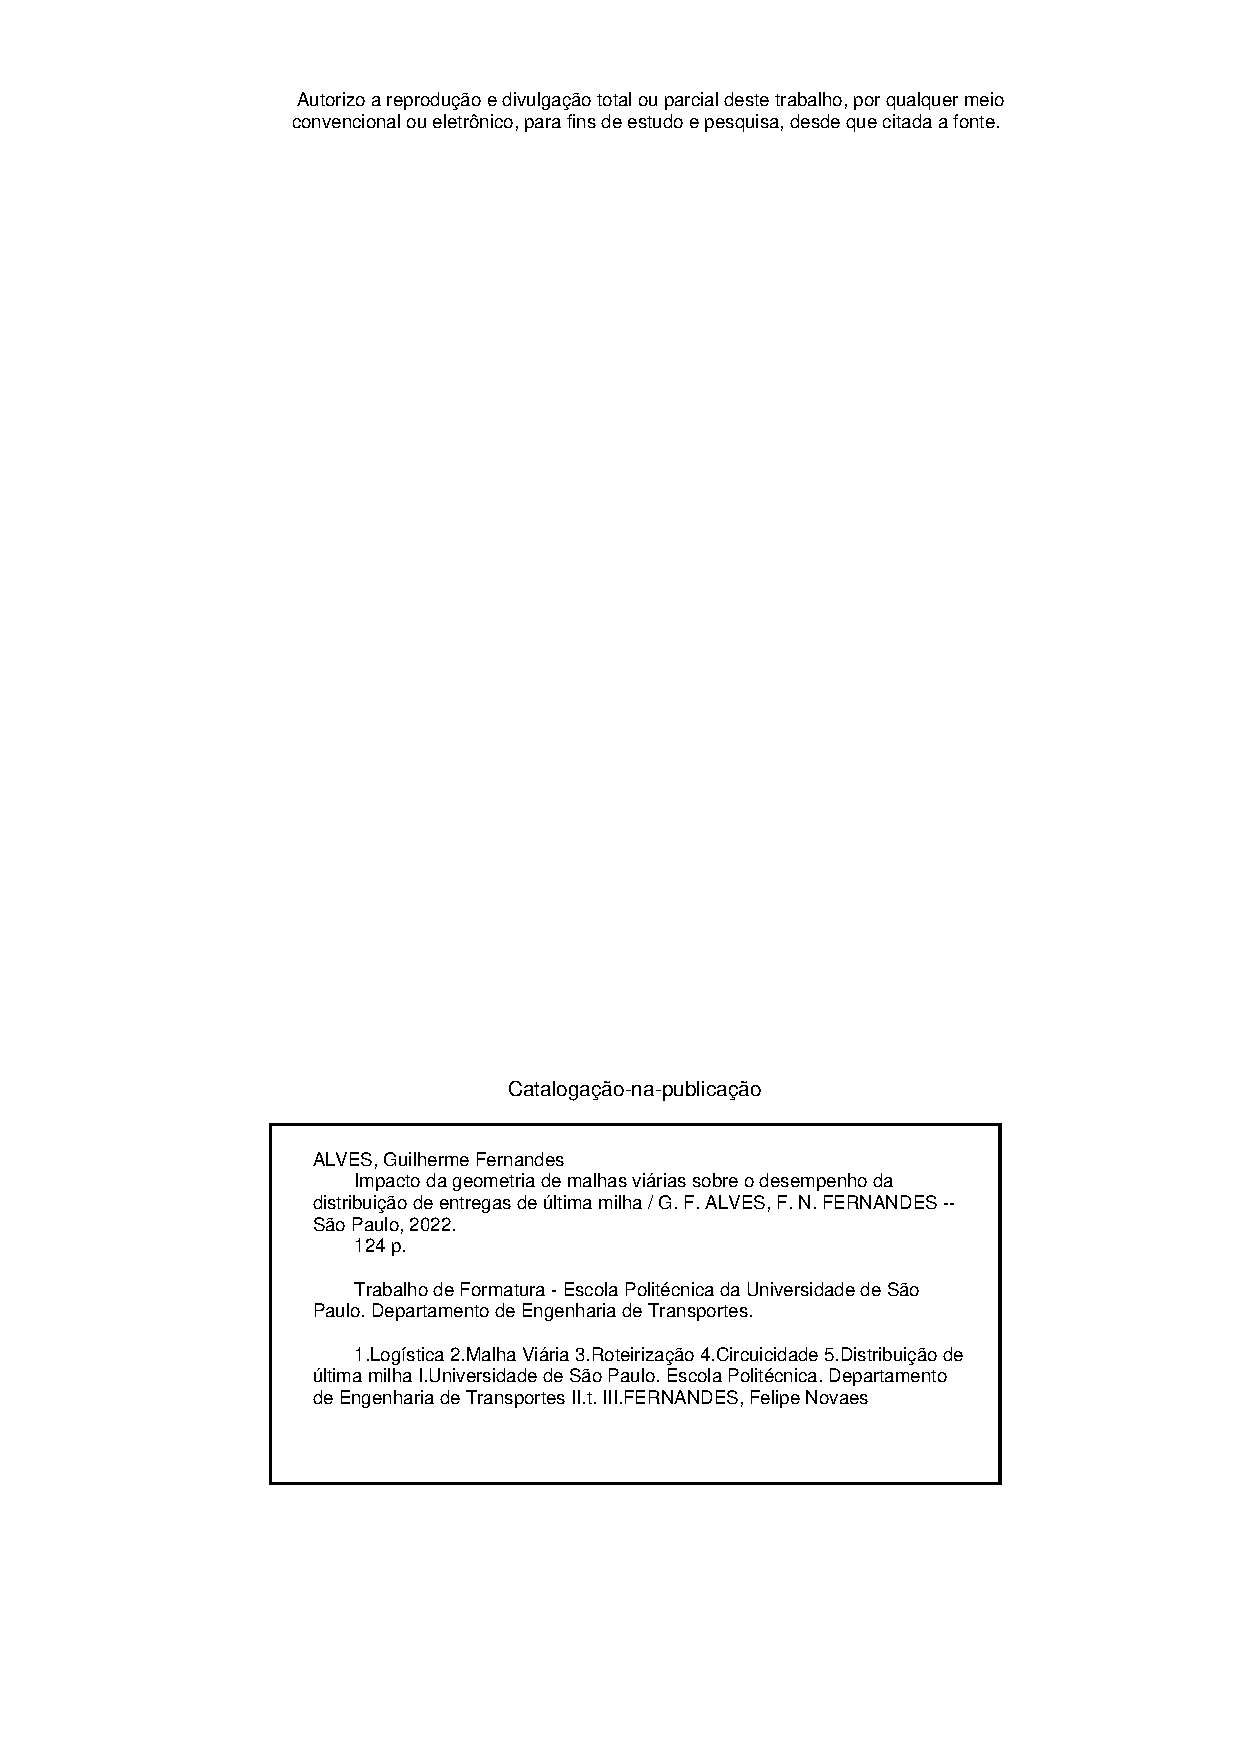
\includepdf{images/catalogacao.pdf}

% ================ Resumo ===============
\begin{resumo}

A distribuição de entregas de última milha em zonas urbanas tem se destacado como uma das atividades mais importantes da logística nos últimos anos.
Caracterizado por abranger a última etapa do processo de entregas de larga escala, o segmento de última milha apresenta uma grande dinamicidade diária, com alto impacto no desempenho das empresas.
Assim, para se aperfeiçoar ou otimizar tal setor, é relevante que se possa ter um bom planejamento tático de suas operações de entrega.
Um problema que se observa, porém, é a diferença entre rotas realizadas e rotas programadas, chamada ``não aderência ao sequenciamento de entregas''.
Essa diferença pode ser avaliada a partir de três indicadores: Repasse, Não Aderência Sequencial e Devolução.
Estes fenômenos compreendem comportamentos inesperados no roteiro de entregas, que implicam em uma série de impactos econômicos, sociais e ambientais.
%
Para que se tenha maior controle sobre a não aderência, é relevante que se tenha conhecimento de quais fatores influenciam sua ocorrência.
O presente trabalho apresenta os primeiros passos para a identificação da correlação entre tais variáveis e diferentes fatores de potencial causalidade.
%
Foram realizados dois estudos de caso com dados reais de entregas de última milha a partir dos Centros de Distribuição respectivos de cada empresa.
Um dos estudos é relativo a uma empresa de bebidas brasileira de grande porte com histórico de entregas na Região Metropolitana de São Paulo, enquanto o outro é do histórico de entregas da \textit{Amazon.com} nos Estados Unidos.
%
Dessa forma, o trabalho permitiu análises de correlação que englobam medidas de caracterização das entregas, de autocorrelação espacial, do posicionamento relativo dos pontos de entrega, do fator de circuito e de um conjunto de variáveis capazes de mensurar diferentes aspectos da geometria de malhas viárias.
% 
A partir dos resultados foi possível identificar efeitos correlatos de aspectos das entregas, tais como o horário da entrega e a equipe que o realiza, assim como com as características associadas à malha viária.
Por meio de regressões lineares simples e múltiplas, foi possível estabelecer que três indicadores associados ao tamanho da rota, ao fator de circuito e à orientação das vias afetam em 18\%, combinadamente, a ocorrência de repasses.
As contribuições do trabalho podem ser úteis para diferentes áreas de estudo, incluindo educação, saúde e gerenciamento de tráfego.
O trabalho se baseou majoritariamente em ferramentas de código aberto disponibilizadas tanto por trabalhos anteriores quanto pelos próprios autores.
Por exemplo, o pacote \textit{lmr\_analyzer} foi escrito em linguagem \textit{Python} e sob demanda para este trabalho, e ao final foi disponibilizado nas principais plataformas de código aberto atuais, permitindo a aplicação dos métodos em outros contextos e também a reprodução dos resultados obtidos.  
\\[3\baselineskip]
%
\textbf{Palavras-Chave} -- Logistics, Last-mile distribution, Vehicle routing problem, Street Network Analysis, Circuity.
\end{resumo}


% ========== Abstract ==========
\begin{abstract}

% In recent years, a sector that has stood out in the logistics area is the \textit{last-mile} segment.
The last mile distribution plays a key role in supply chain management nowadays.
Characterized by covering the last stage of the large-scale delivery process, the last mile segment presents large dynamics on a daily basis, with a high impact on the overall performance of deliveries.
Therefore, in order to either improve or optimize last mile deliveries, it is crucial to have a good tactical planning of your operation.
This paper has ellaborated on top of the phenomena known as ``non-adherence between planned and executed routes'' on last mile distribution.
%
This non-adherence can be evaluated based on three key performance indicators: Failed delivery attempts, Sequential Non-Adherence and Rejections.
These phenomena represent unexpected behaviors in the delivery route and imply in several economic and environmental impacts.
%
With that in mind, to provide a greater control of last mile operations, it is important understand which indicators may influence the occurrence of the non-adherence.
To accomplish with that, this paper presents the first steps towards identifying the correlation between the indicators and different potential causality factors.
%
Therefore, two different case studies with actual data on last mile deliveries were performed. 
One of the studies is related to a large Brazilian beverage company with a database of deliveries in the São Paulo Metropolitan Region (Brazil), while the other is about the delivery database of \textit{Amazon.com} in the United States.
%
Our contributions has allowed for an extensive set of correlation analyzes that address measures of characterizing deliveries routes, spatial autocorrelation, the relative positioning of dropoff points, the circuity factor and a set of variables for measuring different aspects of the street network topology.
%
Furthermore, the results suggests the existence of correlated effects between elements related to deliveries, such as the time of delivery and the delivery team that performs it, as well as characteristics associated with the street network.
After series of both simple and multi-variable regressions, it was possible to establish that three indicators associated with the size of the route, the circuity factor and the orientation may directly affect 18\% of the occurrence of failed delivery attempts.
These contributions may be useful to different study areas, including education, health, traffic management. 
The major part of this work has been based on top of open-source tools provided by previous works and also by the authors.
For instance, the Python module \textit{lmr\_analyzer}, created during this work, is now totally available on open-source platforms, allowing for further investigations under different contexts, as well as the reproduction of this work's results.  
\\[3\baselineskip]
%
\textbf{Keywords} -- Logistics, Last-mile distribution, Vehicle routing problem, Street Network Analysis, Circuity.
\end{abstract}

% ========== Listas (opcional) ==========
\listadefiguras
\listadetabelas
\lstlistoflistings

% ========== Listas definidas pelo usuário (opcional) ==========
\begin{pretextualsection}{Lista de siglas}

\begin{itemize}
    \item ACP: Análise de Componentes Principais;
    \item B2B: \textit{Business-to-business};
    \item B2C: \textit{Business-to-consumer};
    \item CD: Centro de Distribuição;
    \item LISA: Indicadores Locais de Associação Espacial, tradução livre;
    \item NAS: Não Aderência Sequencial;
    \item PDE: Ponto de Entrega;
    \item SKU: \textit{Stock-keeping-unit}, é o código de identificação individual de cada produto;
    \item TSP: \textit{Travelling Salesman Problem};
    \item VRP: \textit{Vehicle Routing Problem}.
\end{itemize}

\end{pretextualsection}

% ========== Sumário ==========
\sumario

% ========== Elementos textuais ==========

\chapter{Introdução} \label{sec:introduction}

O presente documento corresponde ao trabalho de formatura entregue como requisito para obtenção do título de Engenheiro Civil na Escola Politécnica da Universidade de São Paulo.
O trabalho de formatura foi realizado ao longo do ano de 2022 e desenvolvido com base em conhecimentos adquiridos ao longo dos últimos cinco anos de graduação.

O texto trata do problema de roteirização de veículos, do inglês \textit{Vehicle Routing Problem} (VRP), no contexto de distribuição de entregas de última milha em regiões urbanas. 
Mais especificamente, busca-se investigar as causas de rotas realizadas pelos veículos de entrega muitas vezes seguirem uma trajetória diferente da que foi programada previamente.
Essa diferença pode ser tanto em termos de distâncias e tempos, como, principalmente, em termos de alterações na ordem ou sequência de pontos visitado em cada roteiro. Assim, defini-se tal diferença como sendo uma não aderência à roteirização programada.
Ademais, enquadra-se no escopo do trabalho a análise espacial de malhas viárias urbanas, a fim de entender a relação que a geometria da malha tem com essa não aderência supracitada.

%%%%%%%%%%%%%%%%%%%%%%%%%%%%%%%%%%%%%%%%%%%%%%%%%
\section{Objetivos do trabalho} \label{objetivos}

O trabalho teve como objetivo principal estudar o fenômeno de não aderência ao sequenciamento de entregas. Tal sequenciamento ocorre através da roteirização de uma série de clientes associados a uma distribuidora de produtos. Deste modo, define-se a rota formada como todo o percurso contemplado entre a saída de um veículo de entregas de um Centro de Distribuição (CD), passando por cada cliente em ordem sequencial, para realizar a entrega, e, por fim, retornando ao CD para, no dia seguinte, realizar uma nova rota.
Para atender tal objetivo, foram apresentados dois estudos de caso a partir de bases de dados históricos de entregas de última milha.

Primeiramente, estudou-se um conjunto de rotas realizadas por uma companhia de bebidas a partir de um CD localizado na Região Metropolitana de São Paulo, Brasil.
Em seguida, analisou-se a operação de uma empresa de comércio eletrônico, denominada \textit{Amazon.com, Inc}, em cinco grandes centros urbanos dos Estados Unidos.
A análise destes dois estudos de caso facilitou o reconhecimento de padrões a partir dos dados, além de reduzir a possibilidade de existência de algum viés nas considerações finais.

Desta forma uma série de objetivos elencados a seguir foram estipulados.
O primeiro objetivo estipulado é o de definir um conjunto de variáveis associada à distribuição de entregas de última milha, tais como as características do cliente, da equipe de entrega, da entrega em si, da localização do cliente, da rota e da malha viária da região.
Em sequência, o objetivo complementa-se na busca por uma correlação entre a não aderência ao sequenciamento programado e essas variáveis. Tal correlação considera a tese de que a não aderência possa ser explicada através da associação de diferentes fatores associados a essas características.

O primeiro conjunto de fatores estudados são relativos às características próprias da entrega, tais como o horário de entrega, o volume de entrega, entre outros. Tal análise incorpora-se ao objetivo a fim de se compreender a relevância que tais indicadores têm sobre a não aderência ao sequenciamento estipulado.

Em sequência, estudada-se o fator de circuito, o qual será apresentada posteriormente na Seção \ref{sec:fatorCircuito}. 
Tal medida representa a diferença entre a distância euclidiana entre dois pontos localizados numa cidade e a distância real percorrida por um veículo para ir de um desses pontos ao outro. Seu uso, conforme a tese citada, busca mensurar quantitativamente a dificuldade do veículo de entregas de acessar o ponto de entrega e, indiretamente, avaliar a configuração viária da região.

Em adição ao fator de circuito, quantificou-se as características da malha viária a partir de estudos baseados em trabalhos passados.
Estes permitiram acesso a uma gama de parâmetros voltados à caracterização de malhas viárias através da construção baseada em grafos, ou seja, estabelecendo um modelo de grafo que representasse a malha viária e, a partir daí, permitisse que esta fosse quantificada através de determinadas variáveis.
Dessa forma foi possível incorporar novas estatísticas relativas à caracterização da malha viária às análises.

Ademais, a fim de se complementar as análises de malha com a experiência operacional das equipes de entregas de uma das empresas estudadas, realizou-se uma visita técnica a um Centro de Distribuição (CD) de uma das empresas analisadas.
Tal prática permitiu expandir as observações realizadas e confirmar na prática a efetividade de parte das hipóteses, além de captar referências por parte da empresa e de seus operadores, acrescentando assim uma visão prática ao projeto.
%
Assim, complementou-se entre os objetivos do presente estudo  a investigação da interferência de características da malha viária sobre a não aderência do sequenciamento programado de entregas de última milha.

Desta forma, espera-se que o trabalho possa contribuir nas pesquisas futuras acerca da aderência aos resultados de roteirização e sua relação com a malha viária na qual o conjunto de entregas está inserido.
Cita-se, além disso, que as ferramentas e procedimentos utilizados durante a pequisa foram detalhadamente documentados, registrados e, em alguns casos, tornados públicos, a fim de facilitar desenvolvimentos futuros e a eventual reprodução dos resultados.

%%%%%%%%%%%%%%%%%%%%%%%%%%%%
\section{Relevância do tema} \label{RelevanciaTema}

Uma hipótese a ser considerada é a de que os roteiros programados são construídos buscando alguma forma de otimização, seja a minimização de distâncias totais percorridas, de tempo total de entrega ou, então, de custo total para a empresa que realiza essas entregas. 
Sendo assim, ao se realizar uma ou mais rotas de modo diferente do que foi previamente programado, gera-se uma perda de eficiência da operação otimizada de entrega.
Essa perda de eficiência pode ser representada em termos monetários ou não, e impacta diferentes grupos da sociedade.

Primeiramente, nota-se que as próprias empresas enfrentam um aumento de custos devido à não aderência.
Assim, destaca-se o aumento do consumo de combustível, de horas trabalhadas pela mão-de-obra e do custo de manutenção dos veículos, que passam a percorrer distâncias acima do programado e, assim, reduzem seu tempo de vida útil previsto.
Aumenta-se indiretamente, também, o custo total ao se reduzir a capacidade de entregas de cada veículo, ou seja, ao se percorrer distâncias maiores ou gastar tempos maiores para entregas, acaba-se exigindo que um menor número de entregas por veículo seja realizado ou que uma maior frota de veículos seja utilizada.

Além disso, pessoas que moram em centros urbanos e, por consequência, dependem da infraestrutura de malhas viárias, muitas vezes também sofrem com os resultados da não aderência, uma vez que este problema pode acarretar em maiores congestionamentos nas vias por parte dos veículos de entregas que passam a ocupar a via por um tempo maior do que o ideal.
Os funcionários que atuam na operação de entregas também podem ser afetados, uma vez que os atrasos gerados por essa não aderência podem fazer com que a jornada líquida de trabalho se estenda para além do planejado.

Adicionalmente, tem-se o aspecto ambiental.
A emissão de gases contribuidores para o efeito estufa e o aquecimento global é aumentada dado que as distâncias percorridas pelos veículos acabam sendo maiores (assumindo-se uma frota majoritariamente movida a combustão).
Tal efeito é especialmente potencializado em zonas de alta urbanização, que comumente sofrem com a poluição atmosférica.
De fato, algumas cidades europeias têm adotado estratégias de restrição de tráfego de veículos de entrega em zonas centrais da cidade, tornando a distribuição cada vez mais restrita, o que exige por sua vez uma maior eficiência da operação dessas entregas.

%%%%%%%%%%%%%%%%%%%%%%%%%%%%%%
\section{Organização do texto}

Este documento está dividido em \ref{sec:consideracoesFinais} capítulos.
O Capítulo \ref{sec:revis_biblio} apresenta os conceitos utilizados ao longo do trabalho, bem como uma análise sobre a literatura atual e quais oportunidades de melhorias observadas ao se realizar tal análise.

O Capítulo \ref{sec:Contexto} contém uma descrição da operação de cada uma das duas empresas analisadas.
Esta descrição compreende desde aspectos básicos como localização geográfica dos CDs e clientes até aspectos mais detalhados como, por exemplo, o conjunto de dados provindo de cada uma das empresas.

O Capítulo \ref{sec:mat&met} apresenta as metodologias propostas para realização do trabalho, incluindo os resultados esperados que foram elencados no início da pesquisa, as variáveis propostas para quantificar a não aderência ao sequenciamento de entregas, as ferramentais computacionais utilizadas para obtenção e tratamento de dados, os dados geoespaciais empregados e, finalmente, a descrição do conjunto de algoritmos criados durante o trabalho.

Os Capítulos \ref{sec:EstCasoAmbev} e \ref{sec:EstCasoAmazon}  apresentam os resultados obtidos para o exemplo da empresa de bebidas e da \textit{Amazon.com}, respectivamente.
Dentro de cada um desses capítulos são primeiro apresentados os resumos e identificação iniciais dos dados fornecidos, para então descrever-se e quantificar-se o conjunto de rotas e as malhas viárias em que estas estão incluídas. 
Por fim, discute-se a relação entre as variáveis e estatísticas que foram geradas durante cada capítulo.

Finalmente, o Capítulo \ref{sec:consideracoesFinais} descreve as considerações finais do trabalho e é seguido pelas referências bibliográficas.
Logo após as referências, o trabalho é finalizado pelos apêndices adicionados de modo a complementar a argumentação quando necessário.


\chapter{Revisão de conceitos e de bibliografia} \label{sec:revis_biblio}

Neste capítulo descreve-se, primeiramente, o problema de não aderência ao sequenciamento programado e como ele se encaixa no contexto de distribuição de última milha.
Em seguida, serão definidas variáveis de ``circuicidade'', densidade e conectividade no contexto de zonas urbanas, assim como os principais conceitos de regressões lineares.
Tais variáveis e conceitos são apresentados a partir de trabalhos anteriores, que serão mencionados logo em seguida, e, ao longo do presente trabalho, serão utilizados como base para a construção e validação das análises e dos resultados.

Os trabalhos anteriores, que serão mencionados, discorrem acerca da relação entre a rede viária e a eficiência de entregas de última milha, assim como a análise espacial destas malhas por meio de metodologia baseada em grafos. 
Também são descritos alguns dos fundamentos de autocorrelação espacial, que permitirão estabelecer análises de geoestatísticas no decorrer do trabalho. 
Por fim, são apresentadas as considerações finais com respeito à literatura. 

%%%%%%%%%%%%%%%%%%%%%%%%%%%%%%%%%%%%%%%%%%%%%%%%%%%%%%%
\section{Distribuição de última milha em regiões urbanas} \label{sec:definicaoProblema} 

Distribuição de última milha (do inglês \textit{last mile distribution}) refere-se ao último segmento de entrega de mercadorias, ou seja, é a última etapa de uma viagem que vai desde a origem de uma mercadoria até o destino final da entrega.
A distribuição de entregas de última milha em áreas urbanas configura parte importante da engenharia de transportes e também do gerenciamento de cadeias de suprimentos, uma vez que são diversos os estabelecimentos que se beneficiam ou dependem desse tipo de entrega, como supermercados, bares, restaurantes, postos de gasolina, hospitais, entre outros.
Além disso, entregas de última milha em áreas urbanas geralmente são caracterizadas por pequenas distâncias percorridas, elevada quantidade de mercadorias e elevada frequência de entregas, sobretudo em centros urbanos de elevada densidade demográfica.

Empresas que realizam entregas de última milha normalmente enfrentam o problema de roteirização de veículos, que é derivado do termo inglês \textit{Vehicle Routing Problem} (VRP), o qual foi apresentado pela primeira vez por \citeonline{dantzig1959truck}.
De acordo com \citeonline{EKSIOGLU20091472}, a forma clássica do VRP pode ser definida do seguinte modo: 

\singlespacing
\begin{tcolorbox}
\begin{itemize}
    \item Dado um grafo $G=(V,A)$ em que $V$ é um conjunto de $n$ nós em que $V=\{0,1,...,n\}$ e $A$ é o conjunto de arcos;
    \item Os nós $j=1,..., n$ do conjunto $V$ correspondem aos clientes e o nó $j=0$ corresponde ao depósito de origem;
    \item Um custo não negativo é associado a cada arco presente em $A$, sendo que este custo pode representar o tempo ou distância do percurso entre os dois nós que estão conectados pelo arco em questão;
    \item O VRP consiste em encontrar um conjunto de $k$ circuitos (rotas), cada um representando uma rota de mínimo custo, que é definida como a soma de modo que;
    \begin{itemize}
        \item Cada circuito contém o nó $j=0$, ou seja, o depósito;
        \item Cada nó $j$, em que $j \in V\setminus\{0\}$ é visitado por exatamente um único circuito e
        \item a soma das demandas de cada nó em uma rota não supera a capacidade $C$ do veículo.
    \end{itemize}
\end{itemize}
\end{tcolorbox}
\onehalfspacing

A título de observação, quando há somente um único veículo e o objetivo é minimizar a distância total percorrida, o VRP se reduz ao Problema do Caixeiro Viajante, do inglês \textit{Travelling Salesman Problem} (TSP) que por sua vez, de acordo com \citeonline{cookTSP}, não possui uma origem muito bem definida pela literatura. 

Desde a concepção do VRP em \citeyear{dantzig1959truck}, diversas soluções já foram formuladas na literatura, sendo a maior parte delas, segundo \citeonline{BRAEKERS2016300}, baseada em algoritmos de metaheurística, visto que o VRP é um problema de complexidade NP-difícil (\citeauthoronline{garey1976some}, \citeyear{garey1976some}), ou \textit{NP-hard}.
Conforme discutido por \citeonline{arora2009computational}, problemas do tipo \textit{NP-hard} não possuem algoritmo eficiente que resolva, em tempo polinomial, o seu caso mais difícil possível. 
Em outras palavras, conforme o número de pontos a serem visitados aumenta, o esforço computacional empregado para se resolver o VRP cresce exponencialmente, tornando teoricamente impossível a solução ótima quando o número de pontos tende ao infinito. 
% The fact that a problem is NP-hard means that we believe there is no efficient algorithm that solves it in the worst case. It does not, however, mean that every single instance of the problem is hard

Exemplos de metaheurísticas utilizadas para solucionar o VRP podem ser amplamente encontrados na literatura, como é o caso das soluções apresentadas por \citeonline{chiang1997reactive} e \citeonline{homberger1999two}, por exemplo.
Em geral, estes algorítimos baseados em metaheurísticas podem reduzir significativamente o tempo de processamento ao se resolver o VRP (\citeauthoronline{Golden1998}, \citeyear{Golden1998}).
Essa redução de tempo é o que permite que grandes empresas possam otimizar os roteiros de entregas e aumentar o desempenho de suas operações, muitas das vezes atingindo impactos notáveis, como é o caso das aplicações ORION (\citeauthoronline{holland2017ups}, \citeyear{holland2017ups}) e SHORTREC (\citeauthoronline{kant2008coca}, \citeyear{kant2008coca}) desenvolvidas pelas empresas \textit{UPS} e \textit{Coca-Cola}, respectivamente, e que permitiram atingir uma economia anual de \$300 milhões e \$45 milhões de dólares, respectivamente.

Contudo, muitas vezes os resultados das roteirizações não podem ser executados exatamente como programado durante a operação de entregas.
Essa diferença pode ser representada por distâncias adicionais percorridas, tempo adicional de entregas ou até mesmo sequência de visitas em ordem diferente da que foi programada.
A esse fenômeno dá-se o nome de ``não aderência ao sequenciamento programado'', que será o principal objeto de estudo deste trabalho.

%%%%%%%%%%%%%%%%%%%%%%%%%%%%%%%%%%%%%%%%%%%%%%%%%%%%%%%
\section{O fator de circuito} \label{sec:fatorCircuito}
Fator de circuito, ou \textit{circuity factor} em inglês, pode ser definido como a razão entre a menor distância a ser percorrida por um veículo ao ir de um ponto a outro da cidade e a distância euclidiana, isto é, em linha reta entre estes mesmos dois pontos. 
A Equação \ref{eq:fator_circuito} descreve o cálculo do fator de circuito entre dois pontos $p$ e $q$ genéricos.
%
\begin{equation} \label{eq:fator_circuito}
    C_{f_{p, q}} = \frac{(Dist\hat{a}ncia\;Real)_{p, q}}{(Dist\hat{a}ncia\;Euclidiana)_{p, q}}
\end{equation}

Valores de $C_{f}$ podem variar de $1$ até, teoricamente, infinito visto que, para um plano, a distância real percorrida jamais poderá ser menor do que a distância em linha reta entre dois pontos.
Porém é importante destacar que conforme a distância euclidiana aumenta, a distância real percorrida tende a se aproximar cada vez mais da distância em linha reta entre estes dois pontos, conforme ilustrado pela Equação (\ref{eq:limite}).
%
\begin{equation} \label{eq:limite}
    \lim_{Dist\hat{a}ncia\;Euclidiana \rightarrow \infty} \frac{Dist\hat{a}ncia\;Real}{Dist\hat{a}ncia\;Euclidiana} = 1
\end{equation}

De fato, a Figura \ref{fig:FC_julia_artigo} ilustra essa relação assintótica do fator de circuito, onde o eixo das abscissas indica a distância euclidiana e o eixo das ordenadas representa o fator de circuito.
O fator de circuito pode representar a eficiência de locomoção de veículos em zonas urbanas, visto que em geral malhas com fatores de circuito menores representam maior agilidade ao se movimentar por diferentes trechos, ou seja, exigindo menos esforço para se realizar um determinado percurso.

\begin{figure}[H]
    \centering
    \caption{Exemplo de fator de circuito calculado para a cidade de Nova Iorque.}
    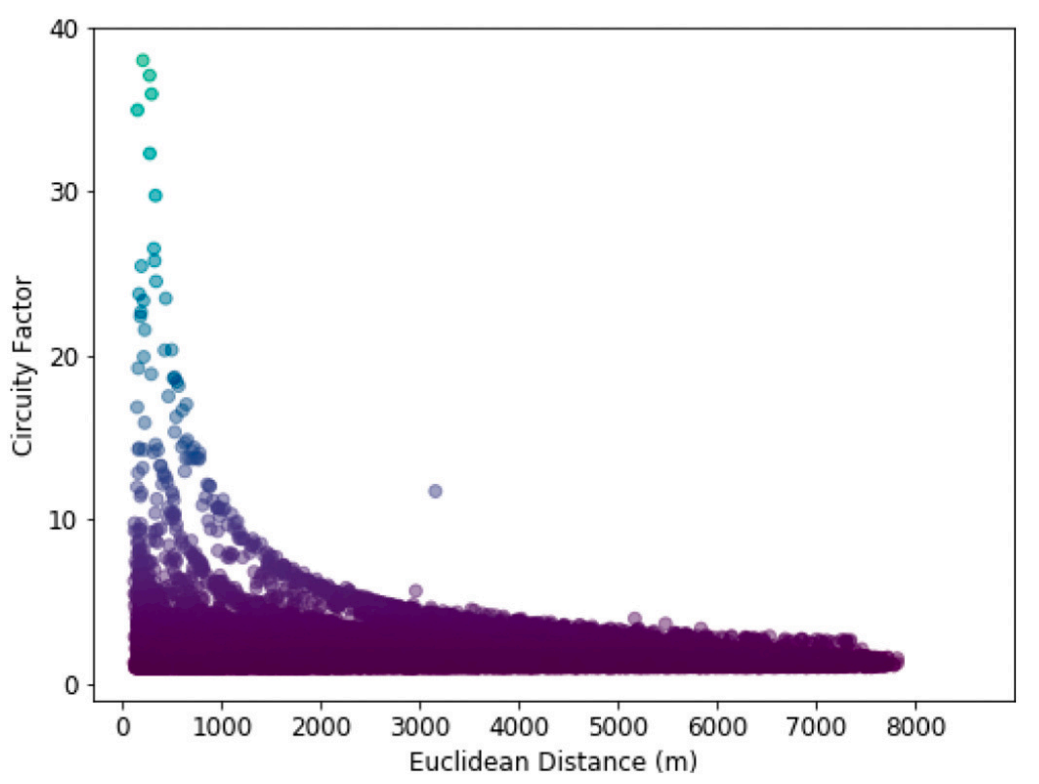
\includegraphics[width=.4\linewidth]{images/2_revisao/julia_fc.png}
    \caption*{\ Fonte: \citeonline{AMARAL2020102916}}
    \label{fig:FC_julia_artigo}
\end{figure}

%%%%%%%%%%%%%%%%%%%%%%%%%%%%%%%%%%%%%%%%%%%%%%%%%%%%%%%
\section{Densidade e conectividade de malhas urbanas} \label{sec:DensConectBiblio}

As medidas descritas nesta seção buscam caracterizar valores com respeito à densidade e conectividade das malhas urbanas, e serão utilizadas com este mesmo propósito ao longo do trabalho.
Densidade se refere à concentração de determinados elementos (e.g. vias e intersecção) na malha urbana, enquanto conectividade refere-se ao quão interligados estão estes elementos da malha viária.
As definições utilizadas podem apresentar variações pela literatura, porém, em geral optou-se por adotar, neste trabalho, a forma padrão de cada um dos indicadores.
Inicialmente apresenta-se o índice de conectividade $C_{index}$ (\citeauthoronline{Marshall_metrics}, \citeyear{Marshall_metrics}), descrito na Equação \ref{eq:conectivity_index} e que representa a razão entre o número de segmentos de vias e o número total de intersecções em uma malha viária.
%
\begin{equation} \label{eq:conectivity_index}
    C_{index} = \frac{n^{\circ}\;de\;Segmentos\;de\;via}{n^{\circ}\;de\;Intersecc\tilde{o}es}
\end{equation}

Também apresenta-se a densidade de intersecções $D_{Intsec}$ (\citeauthoronline{Marshall_metrics}, \citeyear{Marshall_metrics}), que é definida como sendo a divisão entre o número total de intersecções e a área total da malha urbana estudada, conforme descrito na Equação \ref{eq:intersec_density}.
%
\begin{equation} \label{eq:intersec_density}
    D_{Intsec} = \frac{n^{\circ}\;de\;Intersecc\tilde{o}es}{Area}
\end{equation}

Assim como feito para a densidade de intersecções, podemos definir a densidade de vias ($D_{vias}$) como sendo o comprimento total de vias dividido pela área total da malha, conforme a Equação \ref{eq:streets_density}.
%
\begin{equation} \label{eq:streets_density}
    D_{Vias} = \frac{Comprimento \; total \; de \; vias}{Area}
\end{equation}

Por fim, define-se a proporção de vias de mão única ($OW_{ratio}$), a qual reflete o percentual de vias que possuem um único sentido de trafego em relação ao total de vias da malha urbana.  
%
\begin{equation} \label{eq:ow_ratio}
    OW_{ratio}(\%) = 100 \cdot \frac{n^{\circ}\;de\;vias\;de\;m\tilde{a}o\;unica}{n^{\circ}\;de\;vias}
\end{equation}

Quando combinadas, as variáveis apresentadas nesta seção podem fornecer uma descrição preliminar da geometria da malha viária. 
Contudo, posteriormente outras variáveis serão definidas, de modo a ser obter uma descrição mais completa.
Conforme apontado por \citeonline{Marshall_metrics}, algumas dessas medidas de conectividade ($C_{index}$, $D_{Intsec}$ e $D_{Vias}$) podem apresentar inconsistências ao se representar a conectividade de malhas viárias, isso por conta de elas serem funções não lineares da área e geometria das vias. 

%%%%%%%%%%%%%%%%%%%%%%%%%%%%%%%%%%%%%%%%%%%%%%%%%%%%%%%
\section{Regressões lineares} \label{RegressoesLineares}

Tratando-se de regressões lineares simples, \citeonline{Azevedo2016} descreve que para identificar a possível dependência entre duas variáveis $X$ e $Y$, pode-se escrever uma combinação linear tal como apresentada na Equação \ref{eq:reg_linear1}, onde  $Y$ é a variável dependente, $X$ é a variável preditora, $\beta_{0}$ e $\beta_{1}$ são parâmetros de ajuste a serem definidos e $\epsilon_{i}$ é o erro associado ao ajuste da regressão aos dados observados. 
Quanto maior a acurácia da regressão, menor é o valor de $\epsilon_{i}$.
%
\begin{equation} \label{eq:reg_linear1}
    Y = \beta_{0}+\beta_{1}\cdot X+\epsilon_{i}
\end{equation}

\citeonline{Azevedo2016} indica que a chave para a construção de uma regressão linear simples é a definição de $\beta_{0}$ e $\beta_{1}$, os quais podem ser calculados através do métodos de mínimos quadrados (\citeauthoronline{BJORCK1990465}, \citeyear{BJORCK1990465}).
O método dos mínimos quadrados consiste em definir os parâmetros $\beta_{0}$ e $\beta_{1}$ de modo a minimizar o valor absoluto de $\epsilon_{i}$. 
Além disso, ele também define variáveis relacionadas à qualidade da regressão. 
Primeiramente, é estabelecida a soma dos quadrados total (SQT), definida na Equação \ref{eq:reg_linear2}, onde $n$ é a quantidade de observações utilizadas para a construção da regressão. 
Assim, a SQT mensura a variação total de $Y_{i}$.
%
\begin{equation} \label{eq:reg_linear2}
    SQT = \sum_{i=1}^{n} \quad (Y_{i} - \overline{Y})^2 = \sum_{i=1}^{n} \quad Y_{i}^2 - n\overline{Y}^2
\end{equation}

Alternativamente, a variação total de $Y_{i}$ também pode ser representada pela soma dos quadrados dos erros (SQE), conforme apresentado na Equação \ref{eq:reg_linear3}.
%
\begin{equation} \label{eq:reg_linear3}
    SQE = \sum_{i=1}^{n} \quad (Y_{i} - \hat{Y}_{i})^2
\end{equation}

Por fim, ambas as somas SQT e SQE são associadas conforme a Equação \ref{eq:reg_linear4}, tornando possível construir um indicador denominado coeficiente de determinação ($r^2$). 
\citeonline{Azevedo2016} explica que o termo $r^2$ pode ser interpretado como ``a proporção da variação total de Y que é explicada por X, segundo o modelo de regressão considerado.''.
O valor do $r^2$ pode variar de 0 a 1, sendo $r^{2}=0$ um nível total de independência entre $X$ e $Y$, e $r^{2}=1$ um nível total de dependência entre $X$ e $Y$.
%
\begin{equation} \label{eq:reg_linear4}
    r^2 = \frac{SQT-SQE}{SQT}
\end{equation}

Adicionalmente, \citeonline{Chein2019} define regressão linear múltipla, que permite determinar, simultaneamente, a relação que múltiplos preditores (X) têm com a variável dependente (Y). 
Assim, o modelo de regressão linear múltipla é definido como na Equação \ref{eq:reg_linear5}, onde $X_{1}$, $X_{2}$, ..., $X_{k}$ são as $k$ variáveis preditoras do modelo.
%
\begin{equation} \label{eq:reg_linear5}
    Y = \beta_{0}+ \beta_{1} \cdot X_{1} + \beta_{2} \cdot X_{2} + ... + \beta_{k} \cdot X_{k} + \epsilon_{i}
\end{equation}

Assim como feito para as regressões simples, é definido o coeficiente de determinação das regressões múltiplas.
Para tanto, são utilizados os $r^2$ das regressões lineares simples estabelecidas entre os diferentes pares de variáveis Y, $X_{1}$, $X_{2}$, ... e $X_{k}$
A Equação \ref{eq:reg_linear6} apresenta a definição do coeficiente de determinação múltiplo, onde $r_{X_{i}X_{j}}$ é o coeficiente de determinação da regressão linear simples entre $X_{i}$ e $X_{j}$. 
%
\begin{equation} \label{eq:reg_linear6}
    \begin{bmatrix}
    r_{X_{1},X_{2},...,X_{k},Y}^2 
    \end{bmatrix} = 
    \begin{bmatrix}
    r_{X_{1}Y} & r_{X_{2}Y} & ... & r_{X_{k}Y}
    \end{bmatrix} \cdot
    \begin{bmatrix}
    r_{X_{1}X_{1}} & r_{X_{1}X_{2}} & ... & r_{X_{1}X_{k}} \\
    r_{X_{2}X_{1}} & r_{X_{2}X_{2}} & ... & r_{X_{2}X_{k}} \\
    ... & ... & ... & ... \\
    r_{X_{k}X_{1}} & r_{X_{k}X_{2}} & ... & r_{X_{k}X_{k}} \\
    \end{bmatrix}^{-1} \cdot
    \begin{bmatrix}
    r_{X_{1}Y} \\ r_{X_{2}Y} \\ ... \\ r_{X_{k}Y}
    \end{bmatrix}
\end{equation}

Contudo, o coeficiente de determinação da regressão múltipla desconsidera o efeito do número de variáveis preditoras utilizadas na regressão, resultando em valores cada vez maiores de $r^{2}$ conforme se aumenta o número de variáveis, o que pode causar uma falsa afirmação de que as regressões múltiplas necessariamente possuem maior acurácia quando comparado às regressões lineares (\citeauthoronline{Chein2019}, \citeyear{Chein2019}).
Sendo assim, define-se o indicador $r^2_{ajustado}$, o qual considera o número de variáveis preditoras utilizadas no modelo, conforme indicado na Equação \ref{eq:reg_linear7}, onde $n$ é a quantidade de observações utilizadas para construir a regressão e $k$ é o número de variáveis preditoras utilizadas.
%
\begin{equation} \label{eq:reg_linear7}
    r^2_{ajustado} = 1 - (1 - r^2) \cdot \frac{n - 1}{n - k - 1}
\end{equation}

A utilização de regressões lineares pode apresentar diferentes aplicações na Engenharia.
No âmbito deste trabalho, as regressões serão utilizadas em favor de se estabelecer a relação linear entre diferentes variáveis que serão calculadas de modo a quantificar a não aderência ao não sequenciamento de entregas, assim como medidas que quantifiquem a geometria de malhas viárias.
Nesse sentido, a avaliação da acurácia dos modelos empregados, que será feita através dos coeficientes $r^{2}_{simples}$, $r^{2}_{multiplo}$ e $r^{2}_{ajustado}$, será importante para complementar o entendimento sobre os resultados.


%%%%%%%%%%%%%%%%%%%%%%%%%%%%%%%%%%%%%%%%%%%%%%%%%%%%%%%
\section{Analise espacial de malhas viárias} \label{sec:boeingRevBib}

Para caracterizar a geometria de malhas urbanas, é importante combinar diferentes fatores quantitativos e qualitativos.
Conforme apontado por \citeonline{boeing2019urban}, é possível explorar algumas vertentes nesse processo de caracterização: Entropia e Orientação.
Entropia se refere à quantificação do desordenamento das vias presentes na malha em relação à sua disposição espacial (i.e. azimute e comprimento), enquanto que orientação se refere ao padrão de organização das vias, ou seja, se a malha tende a apresentar algum nível de consistência em relação à geometria das vias.

Utilizando a biblioteca \textit{OSMnx} (\citeauthoronline{BOEING2017126}, \citeyear{BOEING2017126}), \citeonline{boeing2019urban} realiza um comparativo de orientação, entropia e configuração de vias dentre cem cidades espalhadas pelo mundo.
Para cada cidade, primeiramente é calculado o azimute de cada via, para tanto é adotada uma representação da malha viária por meio de grafos onde os arcos representam as vias e os nós representam intersecções ou extremos de ruas sem-saída. 
Uma vez calculados os azimutes, os arcos (vias) são divididos em trinta e seis intervalos de $10^{\circ}$, de acordo com seu valor de azimute.
Em seguida, utiliza-se o índice de entropia de \citeonline{Shannon_entropy} para medir a tendência de desordem da distribuição de orientações das vias. 
Com base nos valores de entropia, as cidades são ordenadas e então agrupadas por similaridade. 

A partir dos resultados obtidos, destaca-se a regionalização da configuração e orientação de vias, ou seja, a disposição de malhas urbanas tende a variar substancialmente de acordo com a cidade, país ou continente estudado, revelando assim a necessidade de se entender o contexto local ao se analisar qualquer malha viária.
Ademais, \citeauthoronline{boeing2019urban} aponta que cidades que são mais consistentemente organizadas de acordo com um padrão ortogonal tendem a ter maior conectividade e menor ``circuicidade''.

Sendo assim, o presente trabalho baseou-se nos métodos apresentados por \citeauthoronline{boeing2019urban}, em especial no conjunto de ferramentas disponíveis através do pacote \textit{OSMnx}, de modo a avaliar a característica de malhas viárias quanto à sua organização, orientação e entropia. 
A adoção de tais métodos permite estabelecer novas relações a partir das variáveis de ``circuicidade'' e conectividade apresentadas nas Seções \ref{sec:fatorCircuito} e \ref{sec:DensConectBiblio}, respectivamente. 

%%%%%%%%%%%%%%%%%%%%%%%%%%%%%%%%%%%%%%%%%%%%%%%%%%%%%%%
\section{Relação entre malha viária e entregas de última milha} \label{sec:MalhaViariaBiblio}

\citeonline{merchan2020quantifying} apresentam um estudo sobre a quantificação do impacto de malhas viárias sobre a eficiência de viagens de última milha.
A eficiência de viagens, neste caso, é representada pelo fator de circuito. 
Primeiramente foi utilizada a cidade de São Paulo como estudo de caso e, posteriormente, outras sete cidades foram utilizadas para comparação dos resultados. 
Cada cidade foi dividida em regiões de 1 $km^{2}$ de área, e então calculou-se o fator de circuito médio em cada uma dessas regiões.
Em seguida, variáveis que representam a malha viária foram propostas como potencialmente explanatórias do fator de circuito, sendo elas: densidade de intersecção, comprimento total de vias arteriais, comprimento total de vias coletoras, comprimento total de vias locais, porcentagem de vias de mão única, comprimento médio de segmentos de vias (i.e. distancia média entre quarteirões).
Também foram incluídas variáveis calculadas a partir da biblioteca \textit{OSMnx}, descrita na seção \ref{sec:boeingRevBib}. 

As variáveis explanatórias propostas são primeiramente reduzidas através de uma Análise de Componentes Principais (\citeauthoronline{pearson1901liii}, \citeyear{pearson1901liii}), ou ACP, assim excluindo-se as redundâncias presente nessas variáveis.
A Figura \ref{fig:merchanVariables} apresenta o resultado da ACP, em que é possível destacar que as duas componentes principais são influenciadas principalmente pelo índice de conectividade de nós e porcentagem de vias de mão única.
%
Em seguida, as variáveis resultantes são utilizadas para classificar as regiões de 1 $km^{2}$ de área em três categorias através de um modelo baseado no modelo \textit{Gaussian Mixture Model} (GMM), definido por \citeonline{reynolds2009gaussian}, e no método de agrupamento \textit{k-means} (\citeauthoronline{macqueen1967classification}, \citeyear{macqueen1967classification}).
Dessa forma, são gerados três diferentes grupos - $CL1$, $CL2$ e $CL3$ - de regiões a partir da semelhança apresentada pelos valores das variáveis explanatórias.
A Figura \ref{fig:merchanClusterized} apresenta o resultado da clusterização obtida.
%
\begin{figure}[htbp]
     \caption{Redução e agrupamento com base em variáveis explanatórias. As Figuras estão comprimidas no eixo da primeira componente principal.}
     \begin{subfigure}{.49\textwidth}
         \centering
         \caption{Análise de Componentes Principais (ACP)}
         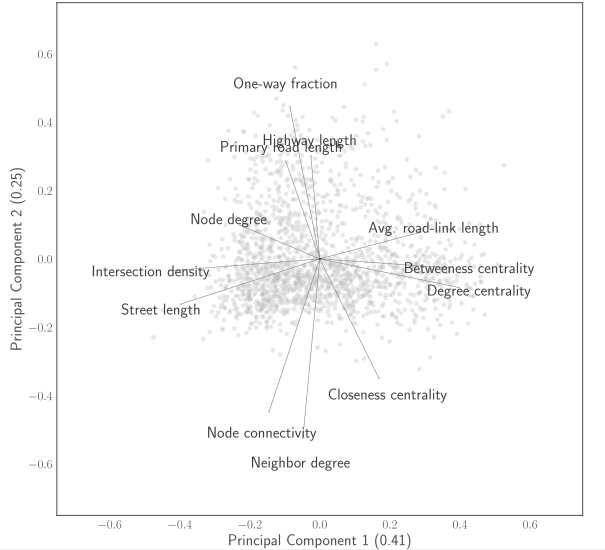
\includegraphics[height=0.75\textwidth]{images/2_revisao/merchan_variables.png}
         \label{fig:merchanVariables}
     \end{subfigure}
     \begin{subfigure}{.49\textwidth}
       \centering
       \caption{Projeção da clusterização sobre a ACP}
       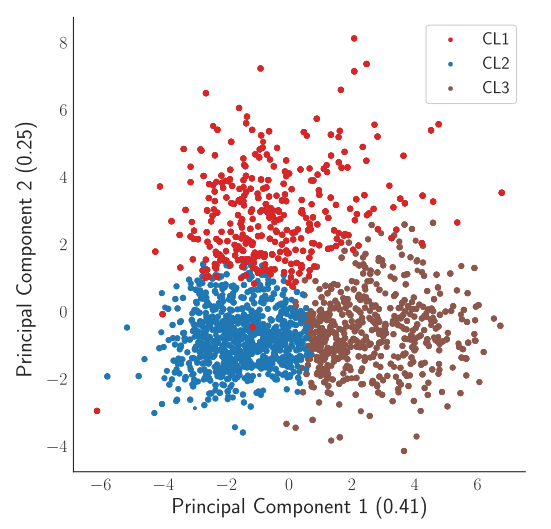
\includegraphics[height=0.75\textwidth]{images/2_revisao/merchan_clusterized.png}
       \label{fig:merchanClusterized}
     \end{subfigure}
     \caption*{\ Fonte: \citeonline{merchan2020quantifying}}
\end{figure}

A distribuição espacial dos três diferentes grupos pode ser observada na Figura \ref{fig:merchanSP}, em que se destaca a presença do grupo $CL3$ em regiões periféricas, e do grupo $CL1$ em regiões centrais.

\begin{figure}[htb]
    \centering
    \caption{Resultado do agrupamento com base nas variáveis explanatórias}
    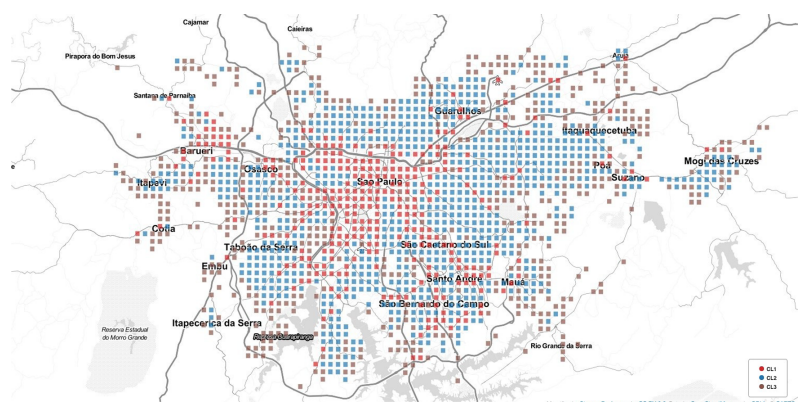
\includegraphics[width=0.9\textwidth]{images/2_revisao/merchan_sp_example.png}
    \caption*{\ Fonte: \citeonline{merchan2020quantifying}}
    \label{fig:merchanSP}
\end{figure}

A partir daí, um modelo de regressão quadrática múltipla é proposto para explicar o fator de circuito a partir das variáveis calculadas, sendo calculada uma regressão para cada grupo $CL1$, $CL2$ e $CL3$.
A determinação dos coeficientes da regressão é realizada através de aprendizagem de máquina, utilizando ferramentas como o \textit{Scikit-learn} (\citeauthoronline{pedregosa2011scikit}, \citeyear{pedregosa2011scikit}).
A partir dos coeficientes, são diferenciadas as variáveis que contribuem para o aumento do fator de circuito (e.g. comprimento de vias, porcentagem de vias de mão única) das variáveis que possuem relação inversa ao fator de circuito, ou seja, que diminuem o valor do fator de circuito quando estas têm seus valores aumentados (e.g. conectividade dos nós).
Por fim, o efeito de cada variável para o valor final do fator de circuito é então discutido, possibilitando a compreensão das considerações finais do trabalho, que podem ser resumidas da seguinte forma:
%
\begin{itemize}
    \item A eficiência de viagens de última milha, neste caso representada pelo fator de circuito, pode ser explicada por uma série de propriedades geométricas e topológicas, algumas das quais podem variar consideravelmente ao longo de uma cidade;
    \item A descrição com base em uma única medida não é suficiente para representar a heterogeneidade da eficiência de viagens de última milha ao longo da cidade, portanto deve-se buscar um conjunto de variáveis que possam descrever diferentes aspectos da malha viária;
    \item A presença de vias de alta capacidade (i.e. rodovias ou vias arteriais) aumenta os valores de fator de circuito no interior das zonas analisadas, que possuem 1 $km^{2}$ de área cada uma.
    Caso fossem analisadas viagens que cruzam a cidade de um extremo ao outro, o resultado seria o oposto: vias de alta capacidade aumentam a eficiência das viagens.
    Ou seja, num contexto de distribuição de última milha, a presença de vias de alta capacidade tende a complicar a eficiência de entregas devido à redução de acessibilidade.
    \item Outros fatores que podem resultar no aumento do fator de circuito são a presença de vias de mão única e a própria topografia local. Por outro lado, malhas viárias de maior índice de conectividade aumentam a acessibilidade e, assim, tendem a apresentar maior eficiência de viagens;
    \item A partir da classificação dos segmentos em três grupos, é possível estabelecer diferentes estratégias de distribuição de entregas, em especial, zonas classificadas como $CL1$ deveriam receber maior atenção ao se projetar sistemas de distribuição de última milha, visto que essas zonas apresentam maiores valores de fator de circuito e maior densidade populacional, implicando em um número maior de entregas sendo realizadas em áreas em que a eficiência de viagens é reduzida.
    \item Um bom entendimento da distribuição espacial do fator de circuito pode contribuir para tomada de decisões em distintas áreas além da logística de distribuição de última milha, tais como o gerenciamento de tráfego e planejamento urbano.
\end{itemize}

%%%%%% Trabalho da Julia: %%%%%%

\citeonline{AMARAL2020102916} também investigaram como a malha viária pode afetar a distribuição de entregas de ultima milha em zonas urbanas, porém desta vez considerando distâncias percorridas, tempo de percurso e topografia da região.
% we propose an approach that allows to identify how the street network within a given urban area may affect last mile distribution in terms of travel distances, travel times and topography
%
São analisadas seis cidades de diferentes continentes e, além disso, é feita uma comparação das velocidades médias de tráfego em diferentes horários do dia.
%
De modo a caracterizar as áreas de estudo, são calculadas variáveis como: densidade de vias ($D_{vias}$), distância média entre quarteirões, densidade de intersecções ($D_{Intersec}$) e porcentagem de vias de mão única ($OW_{ratio}$).
% the following metrics are computed for a preliminary characterization of the study area in terms of its road network: (i) a (iv)

Os resultados obtidos evidenciam a influência que a malha viária exerce sobre as distâncias percorridas em viagens de entregas nas cidades.
% the results we have obtained show that the street network does influence travel distances of delivery trips in the cities.
%
Também pode ser observado que diferentes cidades - as quais possuem diferentes padrões de organização de malha viária - possuem diferentes valores médios de fator de circuito.
% It can also be observed that different cities with different network patterns present different average CFs

Adicionalmente, \citeauthoronline{AMARAL2020102916} explicam que os resultados permitem prever o desempenho da distribuição de entregas nas cidades analisadas. 
% In addition, the results allow a broad comparison between what can be expected from freight deliveries in each city 
%
É citado, como exemplo, que a cidade do Rio de Janeiro possui maior dificuldade de entregas do que as outras cinco cidades estudadas, baseado no maior valor de fator de circuito que essa cidade apresenta.
% For example, it is possible to say that Rio de Janeiro is more challenging for last-mile distribution in terms of traveled distance than the other five cities studied, since it has the highest CFs seen for all distance ranges
%
Nesse sentido, o estudo indica que, durante o planejamento de distribuição de entregas de última milha, uma atenção especial deve ser direcionada para regiões de maior dificuldade de entregas, a fim de se otimizar a eficiência de entregas.
%  at the operational level, special attention should be given to areas deemed as more ‘difficult’ to ensure that the resulting routes are sufficiently robust and less subject to unexpected events
%
Ademais, em relação à evolução da velocidade média dos veículos ao longo do dia, é destacado que em algumas cidades a velocidade média de tráfego tende a variar mais do que em outras e, dessa forma, em determinadas cidades pode ser mais vantajosa a realização de entregas em períodos fora dos horários de pico (e.g. madrugada ou final do dia).  
% Delivery carriers operating in central London, Rio de Janeiro or Bogota would benefit less from switching deliveries to off-hours in terms of vehicle productivity when traveling as travel speed do not increase as much as, for instance, in New York and São Paulo

%%%%%%%%%%%%%%%%%%%%%%%%%%%%%%%%%%%%%%%%%%%%%%%%%%%%%%%
\section{Autocorrelação espacial} \label{sec:autocorrelacaoEsp}

A autocorrelação espacial, como definido por \citeonline{Almeida2012}, busca compreender se existe algum padrão na distribuição espacial dos dados avaliados ou se trata-se de uma distribuição espacialmente aleatória.
A autocorrelação espacial testa a hipótese de que os dados espaciais estão distribuídos aleatoriamente, assim, esta análise faz parte da geoestatística (\citeauthoronline{10.2113/gsecongeo.58.8.1246}, \citeyear{10.2113/gsecongeo.58.8.1246}).

Dentro da geoestatística são estabelecidas diferentes metodologias para a avaliação de autocorrelação espacial dos dados.
A mais tradicional, porém, é a de \citeonline{Moran1948}, que define um coeficiente de autocorrelação espacial conhecido como \textit{I} de Moran.
Sua formulação pode ser observada na Equação \ref{eq:autocor_espacial1}, onde $n$ é o número de regiões utilizadas, $z$ é a variável estudada associada a cada região $i$ e $j$, $W$ é o valor médio das variáveis entre os vizinhos $j$ de $i$ e $S_{0}$ é a média de $z$ globalmente.
%
\begin{equation} \label{eq:autocor_espacial1}
    I = \frac{n}{S_{0}} \cdot \frac{\sum_{i} \sum_{j} W_{ij} Z_{i} Z_{j}}{\sum_{i=1}^{n} Z^2_{i}}
\end{equation}

Sendo assim, a metodologia de \citeauthoronline{Moran1948} busca estabelecer a autocorrelação espacial através do conceito de vizinhança. 
Tal conceito busca compreender, através da variável $z$, se uma região tem algum padrão em relação a seus vizinhos diretos. 
Tal relação é estabelecida a partir da média global ou local a depender da metodologia utilizada.
Na global, categoriza-se cada região como estando acima ou abaixo da média de todos os $z$ observados na área de estudo. 
Já na metodologia local, avalia-se se cada região está acima ou abaixo da média estabelecida entre ela e seus vizinhos diretos.

Após a identificação de cada região em relação à media (global ou local), classifica-se a região de acordo com as seguintes categorias: \textit{Low-Low}, \textit{Low-High}, \textit{High-High}, \textit{High-Low} ou \textit{Indefinido}.
Ao tratar de uma região, por exemplo, que esteja acima da média e seus vizinhos todos abaixo da média, a região é categorizada como \textit{High-Low} e assim por diante.
Se a região não pôde estabelecer algum padrão para com seus vizinhos, ela é classificada como \textit{Indefinida}.
Em termos práticos, \citeauthoronline{Moran1948} permite identificar áreas que possuem padrões de $z$ bem estabelecidos, bem como áreas de baixo padrão espacial (i.e. de disposição geográfica aleatória), que serão classificadas como \textit{Indefinidas}. As representações gráficas dessa classificação das regiões é chamada de Mapa LISA (Mapa de indicadores locais de associação espacial, em tradução livre).

Portanto, a autocorrelação espacial será empregada neste trabalho de modo a investigar a relação entre diferentes zonas, que poderão ser bairros ou cidades, para com os seus vizinhos diretos.

%%%%%%%%%%%%%%%%%%%%%%%%%%%%%%%%%%%%%%%%%%%%%%%%%%%%%%%
\section{Considerações finais sobre a literatura}

Parte dos trabalhos até aqui resultaram em contribuições que evidenciam a interferência das malhas viárias, principalmente com respeito à sua ``circuicidade'', sobre a eficiência das viagens intra urbanas.
Apesar de que algumas outras obras também poderiam ser mencionadas, (e.g. \citeonline{SHEIKHMOHAMMADZADEH2013285}, \citeonline{WANG2020144} e \citeonline{choi2021effect}), a maioria delas trata ou de transporte público urbano ou de viagens de modo automobilístico que não seja relacionado à distribuição de entregas.
%
Além disso, os estudos mencionados na seção \ref{sec:MalhaViariaBiblio} se limitaram a representar a eficiência de entregas de última milha através da medida de fator de circuito, sem de fato entender se essa variável é suficiente para explicar o desempenho dos resultados de roteirizações.

Nesse sentido, não se encontram com facilidade referências que tenham investigado o impacto dessas variáveis sobre a aderência ao sequenciamento programado de entregas. 
Em especial, a literatura deixa espaço para trabalhos que unam a análise espacial de malhas viárias com o desempenho de roteirizações realizadas.
Essa limitação da literatura atual é perfeitamente explicável visto que, se por um lado os dados necessários para a análise espacial são obtidos muitas vezes de banco de dados acessíveis na internet (e.g. \textit{OpenStreetMap}), dados de sequenciamento de entregas são bem mais escassos, visto que estão associados a empresas privadas e que podem conter informações sensíveis tais como o endereço de clientes. 

Em outras palavras, identifica-se a possibilidade de investigação sobre a relação entre os temas de roteirização (\textit{Vehicle Routing Problem}) e disposição espacial de malhas urbanas.
Tal estudo pode contribuir para diferentes áreas de conhecimento, tais como gerenciamento de tráfego, saúde (roteirização de ambulâncias), educação (roteirização de ônibus escolares), entre outros.
Contudo, será dado um foco à distribuição de entregas de última milha, uma vez que esta configura um aspecto menos explorado pela literatura atual.



\chapter{Caracterização das empresas analisadas} \label{sec:Contexto}

Conforme mencionado na Seção \ref{objetivos}, o presente trabalho será constituído de dois estudos de caso com o objetivo de se aplicar a metodologia desenvolvida em situações operacionais de entrega reais.
O primeiro estudo de caso é baseado numa empresa de entregas de bebidas brasileira cuja identificação foi tornada anônima e o segundo é baseado na empresa estadunidense \textit{Amazon.com}. 
Desta forma, o objetivo do presente capítulo é apresentar as características de ambas as empresas de modo a contextualizar as análises, hipóteses e resultados obtidos nos capítulos posteriores.

%%%%%%%%%%%%%%%%%%%%%%%%%%%%%%%%%%%%%%%%%%%%%%%%%%%%%%%%%%%%%%%%%%%%
\section{Empresa de bebidas brasileira} \label{sec:realidade_empresa}

Diferentemente do segundo estudo de caso, sua identificação teve de ser tornada anônima devido às especificidades do caso.
O estudo foi estabelecido através de uma base de dados histórica fornecida e uma visita técnica realizada a um de seus CDs, que serão apresentados a posteriori.

A empresa é caracterizada por se destacar internacionalmente na fabricação e distribuição de bebidas, com grande relevância na indústria alimentícia nacional.
Sua operação é caracterizada por uma diversidade de instalações (fábricas, CDs, armazéns, etc.) e um portfólio de diversos produtos ou \textit{Stock-Keeping-Units} (SKUs) diferentes, contando com mais de 30 mil funcionários no Brasil e uma produção de mais de 15 bilhões de litros de bebidas por ano.
Os clientes da empresa são majoritariamente bares, restaurantes e supermercados. Sendo assim, a distribuição de última milha da empresa pode ser caracterizada como \textit{Business-to-business} (B2B), visto que os clientes não são os consumidores finais dos produtos.

A empresa atual nos diferentes processos da indústria de bebidas, desde a sua fabricação até a entrega final nos bares, restaurantes e locais de venda em geral.
Assim, sua operação logística é caracterizada por um nível de complexidade elevado associado a várias etapas  de deslocamento, desde a saída das fábricas de bebidas até o cliente.
Tais etapas contam com diferentes níveis de planejamento e intensidade operacional, marcados por volumes grandes e percursos longos nas etapas de transferências entre instalações físicas, por exemplo, e volumes pequenos, em veículos urbanos com distância reduzidas, na etapa final de entregas, por exemplo.
A etapa final de entregas é o trecho entre o CD final de armazenamento (normalmente localizados perifericamente às grandes aglomerações urbanas) e os clientes finais.
Assim, cita-se a operação como bastante volátil a depender dos clientes e de suas oscilações de consumo e mais pulverizada, considerando-se a alta quantidade de pontos de entregas finais que devem ser, na maioria das vezes, atendidos com veículos menores devido às regras de circulação dos centros urbanos.

Tal etapa, em maior detalhamento, é realizada a partir de diversos CDs no Brasil, podendo, em certas circunstâncias, ter mais de um CD para a mesma região urbana.
Esse é o caso da Região Metropolitana de São Paulo.
Nela, a empresa situa-se através de um conjunto de CDs localizados nas regiões mais periféricas, devido ao custo fixo das instalações ser mais reduzido.
Cada CD é responsável por uma parcela geográfica da Região Metropolitana, de modo a satisfazer toda a demanda pulverizada dos municípios que a compõe.
O presente trabalho estuda dois CDs presentes na Região Metropolitana citada, a fim de se aplicar a metodologia desenvolvida nessa última etapa de entregas da empresa.
O primeiro CD é estudado através de uma visitação técnica realizada pelos Autores no início da pesquisa.

Ao longo da visita pode-se contemplar o passo a passo pelo qual se dá a rota de entregas de um dos veículos padrão do CD em associação com a observação dos comportamentos e tomadas de decisões dos clientes, da equipe de entregas e da equipe de supervisão.
Nesse aspecto, cita-se que a empresa conta com uma estrutura hierárquica bastante marcada e, no caso da entrega existem três cargos relevantes a serem citados. 

O primeiro cargo é o de supervisor de rotas. Seu trabalho é manter o controle e o contato direto com todas as equipes de entrega pelas quais ele é responsável.
Eles dispõe de veículos próprios para acompanhamento presencial das equipes e utilizam o telefone como plataforma básica de comunicação e acompanhamento. Em geral, no CD em questão, os supervisores de rota são responsáveis por 20 a 30 equipes de entrega cada um.
Em sequência, há os dois cargos das equipes.

O segundo cargo é o de motoristas. 
O motorista é tido como o líder da equipe responsável pela direção do veículo, controle da rota de entregas e principal tomador de decisões.
Normalmente, o motorista é o mais experiente da equipe e é o que mantém contato direto com o supervisor e com o cliente.

Por fim, a equipe é complementada com os ajudantes.
Cada equipe conta com pelo menos um ajudante, sendo que pode haver um segundo caso a rota de entregas do dia tenha mais de 230 caixas a serem entregues.
O ajudante costuma ser o mais inexperiente da equipe, cujas responsabilidades são associadas ao trabalho mais manual da entrega, realizando a abertura do caminhão, a separação dos produtos do cliente em questão, a entrega em si e o fechamento do caminhão.
Sua relação direta é estabelecida mais com o motorista da equipe, mas o responsável formal pelos ajudantes é o supervisor.

Assim, a visitação técnica realizada visou conhecer mais detalhadamente o planejamento tático de roteirização das entregas, bem como as características e nuances presentes no cotidiano da operação.
Tratando-se de um mercado de alta demanda, toda a rotina operacional de entregas apresenta ciclicidade diária, geralmente funcionando de segunda a sábado e integrando diversas áreas da empresa que contribuem com distribuição de última milha.

O segundo CD estudado é compreendido através de uma base de dados histórica das rotas de entregas de todos os seus veículos num período de 5 meses (entre janeiro e maio de 2015).
Sua operação de entregas é numa área que engloba três cidades da Região Metropolitana de São Paulo.
O CD conta com uma operação de larga escala  baseada em mais de 40 veículos e mais de 4.500 clientes atendidos.
Assim, ele é parte essencial da composição final de entregas das bebidas na maior região metropolitana do Brasil. 

Identifica-se que a base contempla 4.554 clientes diferentes, que serão aqui identificados como Ponto de Entrega (PDE).
Estes clientes são identificados cada um com um número aleatório diferente, de modo a se preservar o anonimato de cada PDE.
%
Ademais, a base apresenta um conjunto de 42 veículos de entrega, cada um identificado por um número aleatório que representa o número da placa do veículo.

No total observa-se uma média de 694 PDEs atendidos por dia, a partir de uma média de 38,85 veículos utilizados por dia, durante um período total de 124 dias.
Assim, a base concretiza-se com um total de 88.338 entregas, as quais estão divididas em rotas.
Uma rota é única para cada dia, veículo e conjunto de clientes, portanto se um mesmo veículo atender exatamente os mesmos clientes em dois dias seguidos, serão consideradas duas rotas distintas.

A base é discretizada na chave de entregas, apresentando informações relativa a cada entrega realizada ao longo do período descrito.
Cada entrega é relacionada com 42 variáveis identificatórias e descritivas que singularizam cada entrega.
A principal variável presente na base diz respeito à ordem programada e ordem real de cada entrega na rota, assim permitindo a comparação entre rotas programadas e rotas realmente realizadas.

Uma limitação que pode ser observada na base é a falta de informações relativas ao PDE e à equipe (motorista e ajudante(s)) de entrega.
No total, no que tange o PDE, dispõe-se apenas do código identificador unitário e das suas coordenadas geodésicas decimais (latitude e longitude), limitando a compreensão mais aprofundada das características relativas a cada ponto de entrega, embora preserve o anonimato dos clientes.
O volume e a frequência de entregas, porém, são informados, o que permitirá atribuir noções indiretas de tamanho e relevância de cada PDE. 
No que tange a equipe de entregas, sabe-se, apenas, a placa do veículo que realizou cada rota.
Ademais, a informação de capacidade de cada veículo não foi divulgada.

Uma dificuldade adicional enfrentada foi a falta de precisão aplicada às informações geográficas.
A base conta com três dados de localização para cada PDE que influenciam diferentemente cada resultado.
Esses valores variam dado que um mesmo PDE pode ser atendido em mais de um dia e, assim, ter coordenadas de entregas cadastradas levemente diferentes.
Em outras palavras, a cada dia em que se realiza uma entrega, o veículo pode estacionar em uma posição distinta da rua, e, assim, registrar como coordenadas de entrega um valor diferente. 
Todavia, uma média das coordenadas registradas na base foi utilizada de modo a facilitar o estudo. 

Adicionalmente, a Tabela \ref{tab:Variaveis_BD}, disponível na seção apêndice \ref{sec:AppBDAmbev}, ilustra as variáveis apresentadas na base, bem como o intervalo de valores de cada uma das variáveis.

%%%%%%%%%%%%%%%%%%%%%%%%%%%%%%%%%%%%%%%%%%%%%%%%%%%%%
\section{Empresa americana \textit{Amazon.com, Inc.}}

Enquanto se aproximavam da segunda metade do trabalho, os autores se depararam com a oportunidade de entrar em contato com uma base de dados históricos de entregas de última milha nos Estados Unidos de uma das maiores empresas de comércio eletrônico no mundo, a \textit{Amazon.com, Inc.}.
A empresa apresenta uma das operações de entregas mais complexas do planeta, contando com fornecedores primários e clientes finais presentes em mais de 19 países em todos os continentes. Assim, como cita \citeonline{Holden2020}, a empresa é altamente dependente de otimização de rotas, a fim de se maximizar produtividade da empresa.

Assim como na empresa anterior, sua operação é estabelecida em uma sequência de etapas desde a saída do produto do local de despacho até a recepção do cliente final.
Assim, a empresa conta com uma gama de políticas específicas à operação de cada região e de cada classe de produtos.
Em exemplo, cita-se os produtos de alta demanda que, em muitos casos, já ficam à disposição nos CDs finais das regiões de grande consumo para garantir entregas de curto prazo ao custo de um armazenamento maior e uma estrutura logística \textit{inbound} do CD com maior complexidade.
Após a saída do CD, os produtos a serem entregues diariamente nas regiões altamente urbanizadas estão sujeitos a rotas de maior densidade.
Os caminhões da Amazon transportam mais de 2.000 caixas por rota, como cita \citeonline{Taylor2019}.

Preocupada em otimizar seu desempenho operacional, a empresa publicou em 2021, sob parceria com o \textit{Massachusetts Institute of Technology} (MIT), um desafio global de roteirização.
O desafio em questão visava estimular a contribuição por parte do meio acadêmico para a operação da empresa, permitindo que diversos modelos e propostas de melhorias pudessem ser testados.
Algumas dessas propostas foram consolidadas e então publicadas por \citeonline{winkenbach2021technical}. 

Adicionalmente, destaca-se que a dinâmica de entregas da empresa norte-americana se diferencia da empresa brasileira. 
Primeiro, cita-se que a Amazon contempla distribuição de entregas de modelo \textit{Business-to-consumer} (B2C), em que os receptores das entregas são os consumidores finais, enquanto o primeiro estudo de caso se encaixava no modelo B2B.
Além disso, os casos também diferenciam-se devido ao volume e dimensões dos pacotes entregues, bem como pela segurança da entrega.
Nos Estados Unidos, o cliente pode, em geral, contar com a segurança da entrega sem a necessidade de estar presente para assinar a recepção do bem, algo que no Brasil não se aplica.
Além disso, cita-se que os casos diferenciam-se, também, pelos meios de pagamento.
As entregas de bebidas analisadas no primeiro estudo se caracterizavam pelo fato de o pagamento da nota fiscal ser realizado instantes antes da entrega ser efetivada, geralmente logo depois que o veículo se apresenta à portaria do cliente.
Com o a empresa estadunidense, contudo, os pagamentos já estão confirmados desde instantes após a compra, não correndo o risco de alguma entrega ser devolvida por indisponibilidade do cliente em realizar o pagamento.

Ademais, como citado, foi obtida uma base de dados histórica da operação de entregas da empresa através do desafio global de roteirização que publicou em 2021.
Estas entregas contemplam diferentes produtos, de diferentes dimensões, não somente bebidas.
A base está publicada pelo programa de dados abertos - \textit{Open-data} - da empresa e a descrição detalhada da estruturação dos dados é apresentada por \citeonline{amz_lmrc_Merchan2022}.
Destaca-se que, por fazer parte de um programa de dados abertos, a organização destes conjuntos de dados, bem como a precisão das informações, superam com facilidade a base de dados estudada anteriormente.

A única limitação, porém, é que neste caso não estão disponíveis os dados de rotas programadas, ou seja, conta-se apenas com um histórico de rotas de entregas realizadas para determinadas regiões durante um determinado período de tempo.
Uma descrição completa dos dados fornecidos pode ser encontrada na seção de apêndice \ref{sec:appDBAmazon}.

\chapter{Materiais e Métodos} \label{sec:mat&met}

No presente capítulo introduz-se o conjunto de metodologias utilizadas ao longo do trabalho para a construção das análises e dos resultados obtidos em ambos os estudos de caso apresentados nos Capítulos \ref{sec:EstCasoBebidas} e \ref{sec:EstCasoAmazon}.
Partes das  metodologias utilizadas no trabalho já foram descritas no Capítulo \ref{sec:revis_biblio} como partes das referências conceituais utilizadas no trabalho. Assim, serão devidamente referenciados sempre que utilizados.
Por outro lado, parte das metodologias desenvolvidas foram construídas para o desenvolvimento do presente trabalho, tornando conveniente a explicação das motivações e hipóteses adotadas.

Na Seção \ref{sec:variaveis_do_problema} inicia-se o capítulo a partir da quantificação do problema estudado através de variáveis mensuráveis nos estudos de caso.
Tal seção tem como objetivo estabelecer a base das análises realizadas nos estudos de caso.

Posteriormente, na Seção \ref{sec:ferramentas}, apresenta-se as ferramentas utilizadas ao longo do trabalho, tais como a linguagem de programação \textit{Python}, os softwares de análise georreferenciada \textit{QGIS} e \textit{GeoDa} e, por fim, o editor de planilhas digitais \textit{Excel}.

Adiante, na Seção \ref{sec:dados_de_informacao_geografica}, são apresentadas as bases de dados georreferenciadas utilizadas para a concepção de algumas análises. Entre elas, cita-se os mapas georreferenciados dos bairros de cada cidade estudada nos estudos de caso. A seguir, na Seção \ref{GeoDa}, apresenta-se as metodologias utilizadas dentro da ferramenta \textit{GeoDa} para a construção das análises geoestatísticas realizadas. Em seguida, na Seção \ref{sec:dispGeoRotas} apresenta-se a metodologia desenvolvida para a análise da dispersão geográfica das rotas, que, em suma, busca avaliar o posicionamento dos PDE em relação aos outros PDEs da mesma rota de entregas.

Por fim, na Seção \ref{BibLMRA}, apresenta-se a concepção de toda a metodologia utilizada em \textit{Python} para a construção da biblioteca \textit{Last-Mile-Routing-Analyzer}. Essa biblioteca, publicada abertamente na plataforma Github (\citeauthoronline{guilherme_fernandes_alves_2022_6792977}, \citeyear{guilherme_fernandes_alves_2022_6792977}), é responsável por um conjunto de procedimentos, desde a abertura e organização das bases de dados, até análises relativas à estrutura viária.

Ademais, é possível definir as hipóteses preliminares que foram estabelecidas no início do projeto.
Estas premissas foram importantes para que o trabalho tivesse ao menos um direcionamento quanto às linhas de pesquisa que deveriam ser aprofundadas durante execução do trabalho.
%
\begin{enumerate}
    \item A configuração das vias pode fazer das cidades lugares mais ou menos complexos para entregas de distribuição de última milha, sendo que as condições de terreno também podem afetar essa complexidade (relevo, elevação, etc.);
    \item Por meio de abordagens vistas na literatura, será possível quantificar essas condições adversas de diferentes malhas urbanas, permitindo comparações baseadas em estatísticas e ao mesmo tempo facilitando investigações de correlações ou de relação causa x consequência;
    \item Verificar se regiões em que as rotas realizadas apresentam menor aderência ao sequenciamento programado apresentam também piores valores de fator de circuito ou outras medidas;
    \item Avaliar se, ao quantificar a malha viária de um centro urbano através de diferentes medidas, é possível inferir quais seriam as regiões de pior aderência ao sequenciamento programado. 
\end{enumerate}

Espera-se que ao final do trabalho possa se confirmar parcial ou completamente as hipóteses preliminares que foram descritos nesta seção.

%%%%%%%%%%%%%%%%%%%%%%%%%%%%%%%%%%%%%%%%%%%%%%
\section{Medidas da não aderência às roteirizações programadas} \label{sec:variaveis_do_problema}

Para se obter uma perspectiva quantitativa baseada em dados, foram definidas variáveis contínuas que representem a não aderência ao sequenciamento programado de entregas.
A partir dessas variáveis foi possível mensurar e analisar correlações entre medidas associadas à não aderência e qualquer outra medida escolhida, seja de ``circuicidade'', conectividade, ou outras.

Ademais, foi importante contar que as variáveis propostas puderam ser calculadas a partir das bases de dados históricos utilizadas no trabalho. 
Ademais, essas medidas foram simples o suficiente a ponto de permitir a quantificação do fenômeno de não aderência tanto para o caso da empresa de bebidas quanto para o caso da \textit{Amazon.com}.
Não obstante, espera-se que as medidas propostas poderão ser utilizadas também em trabalhos futuros que considerem estudos de casos similares, independente da empresa analisada.

A seguir, são descritas as três variáveis propostas para quantificar o fenômeno de não aderência: Repasse, Devolução e Não Aderência Sequencial (NAS).
Essas medidas foram utilizadas ao longo do trabalho para investigar se há alguma consistência ou recorrência de repasses em PDEs ou rotas específicas, a fim de se identificar regiões que deveriam receber maior atenção durante o planejamento de rotas de entregas.

%%%%%%%%%%%%%%%%%%%%
\subsection{Repasse}
 
Repasses são eventos inesperados que levam a equipe de entregas a realizar mais de uma visita ao mesmo PDE numa mesma rota. 
Em tais situações, identifica-se que por algum motivo a equipe é incapaz de realizar a entrega na primeira visita que realiza ao estabelecimento naquele dia.
Os repasses podem ocorrer por diversos motivos, dentre eles, destaca-se: o cliente estar ausente, o estabelecimento estar fechado (no caso de entregas B2B) e o cliente não possuir dinheiro suficiente para realizar o pagamento quando este é realizado durante a entrega (também B2B).

Deste modo, define-se a variável repasse como sendo o percentual de visitas, de acordo com a Equação \ref{eq:repasse}.
Nota-se que a medida de repasse pode ser calculada sobre um PDE, rota, área ou intervalo de tempo, assim permitindo diferentes análises a partir de uma única variável.
%
\begin{equation} \label{eq:repasse}
    Repasse (\%) = 100 \cdot \frac{n^{\circ} \; de \; repasses}{Total \; de \; entregas}
\end{equation}


%%%%%%%%%%%%%%%%%%%%%%
\subsection{Devolução}

Diferentemente do repasse, as devoluções acontecem quando a equipe de entregas, por alguma razão, não consegue realizar a entrega programada e acaba devolvendo as mercadorias para o CD.
Uma das causas de devoluções é a rejeição de mercadorias por parte do cliente, o qual pode identificar que o pacote não está em condições adequadas, ou que a entrega não contém exatamente os produtos que foram pedidos, ou até mesmo pode ser alegado que o endereço programado para entrega não corresponde ao endereço do cliente.
%
Outra causa das devoluções é a impossibilidade de entregas devido ao fim do expediente da equipe de entregas, muitas das vezes ocasionada por atrasos ocorridos em outras entregas da rota.

É possível definir uma variável de devolução como sendo o percentual de mercadorias (ou pacotes) devolvidas em relação ao total de mercadorias que deveriam ser entregues, conforme a Equação \ref{eq:devolucao}.
%
\begin{equation} \label{eq:devolucao}
    Devoluc\Tilde{a}o (\%) = 100 \cdot \frac{n^{\circ} \; de \; pacotes \; devolvidos}{Total \; de \; pacotes}
\end{equation}

%%%%%%%%%%%%%%%%%%%%%%%%%%%%%%%%%%%%%%%%%%%
\subsection{Não Aderência Sequencial (NAS)}

A terceira variável proposta é a Não Aderência Sequencial (NAS), que identifica os casos em que o pedido do PDE é entregue numa posição sequencial da rota diferente da planejada. 
Em exemplo, uma situação de NAS pode ser um caso em que a equipe de planejamento estabeleceu que determinado PDE seria a 4ª entrega de determinada rota mas, no instante da entrega, a operação opta por tornar o PDE o 6º a ser visitado naquele dia.

Nesse sentido, para cada entrega estabelece-se uma variável binária indicando se a entrega foi realizada na sequência programada ou não.
A partir daí, pode ser definida uma variável global de NAS como na Equação \ref{eq:NAS}.
%
\begin{equation} \label{eq:NAS}
    NAS(\%) = 100 \cdot \frac{n^{\circ} \; de \; etregas \; em \; sequencia \; diferente \; da \; programada}{Total \; de \; entregas} 
\end{equation}

%%%%%%%%%%%%%%%%%%%%%%%%%%%%%%%%%%%%%%%%%%%%%%
\section{Ferramentas} \label{sec:ferramentas} 

Ao longo do trabalho foram utilizados diversos recursos tecnológicos a fim de possibilitar o desenvolvimento das análises.
%
As ferramentas utilizadas configuram parte importante do conhecimento adquirido durante a graduação no curso de Engenharia Civil da Escola Politécnica.

Primeiramente destaca-se utilização da linguagem de programação \textit{Python} (\citeauthoronline{van1995python}, \citeyear{van1995python}) em sua versão 3.9, que permitiu a leitura de bases de dados e posterior tratamento das informações, representando parte importante da ciência de dados empregada durante o trabalho.
%
Além disso, ao utilizar rotinas escritas em linguagem \textit{Python} foi possível integrar dados provindos de banco de dados distintos por meio de bibliotecas dedicadas.
%
Destaca-se aqui a utilização das bibliotecas \textit{googlemaps} (versão 4.6.0) e \textit{osmnx} (versão 1.2.1), que permitem acesso às informações disponíveis nas plataformas \textit{Google Maps API}, e \textit{OpenStreetMap} (\citeauthoronline{OpenStreetMap}, \citeyear{OpenStreetMap}), respectivamente.
Com superior destaque para a \textit{OSMnx}, que também permitiu uma série de análises quanto à geometria e arranjo de diferentes malhas viárias.
% TODO: Falta uma citação do Google Maps aqui

No âmbito de sistemas de informações geográficas, foi utilizado o \textit{software} de código aberto \textit{QGIS} (\citeauthoronline{QGIS_software}, \citeyear{QGIS_software}), que é um aplicativo de código aberto que permite o tratamento de informações dados espaciais, bem como elaboração de mapas e representações dos dados georreferenciados.
Também foi utilizado o programa de código aberto \textit{GeoDa} (\citeauthoronline{anselin2010geoda}, \citeyear{anselin2010geoda}), que permitiu a aplicação de conceitos de geoestatística sobre os dados espaciais analisados.
 
Por fim, ressalta-se a importância do editor de planilhas digitais \textit{Excel} (\citeauthoronline{msexcel}, \citeyear{msexcel}), da empresa \textit{Microsoft}, que na presente pesquisa foi utilizado, essencialmente, para os procedimentos de armazenamento, tratamento, construção, análise e visualização de dados. 
Podendo estes dados ser referentes às bases fornecidas para os estudos de caso ou aos dados gerados a partir das análises. 

%%%%%%%%%%%%%%%%%%%%%%%%%%%%%%%%%%%%%%%%%%%%%%
\section{Dados de informação geográfica} \label{sec:dados_de_informacao_geografica}

%%%%%%%%%%%%%%%%%%%%%%%%%%%%%%%%%%%%%%%%%%%%%%%%%%%%%%%%%%%%%
\subsection{Guarulhos-SP, Brasil} \label{sec:georef_guarulhos}

Para elaboração do trabalho foi utilizado um arquivo em formato \textit{shapefile} contendo os limites de bairros da cidade de Guarulhos, que representa a maior parcela da região analisada no primeiro estudo de caso analisado.
%
Apesar de o CD da empresa atender também outras cidades como Itaquaquecetuba e Arujá durante a série histórica analisada, somente a cidade de Guarulhos foi selecionada para análises de mapeamento, uma vez que estas outras cidades carecem de dados mais acurados quanto aos limites de bairros e outras informações.

Este arquivo \textit{shapefile} tem sua origem no banco de dados da plataforma \textit{OpenStreetMap}, porém foi extraído através do \textit{software} \textit{QGIS} descrito na seção \ref{sec:ferramentas}. 
%
Após a sua obtenção, identificou-se um conjunto de falhas em sua composição.
%
Primeiro, identificou-se a presença de dois bairros localizados fora dos limites municipais de Guarulhos.
%
Em sequência, identificou-se que nove bairros estavam ausentes, formando espaços vazios no interior polígono e, por fim, dois dos bairros estavam com formatos inadequados quando comparados com um mapa da região.
%
Assim, através do \textit{QGIS} foi possível corrigir todos os problemas e, estabelecer uma base completa dos 47 bairros do município. 
%
A Figura \ref{fig:GRU_shapefile_QGIS} apresenta os bairros já corrigidos, enquanto que a Figura \ref{fig:GRU_shapefile} mostra como os dados estavam disponibilizados previamente.
%
Cita-se que para a construção dos bairros faltantes, utilizou-se como base as definições presentes no site da prefeitura local.
% TODO: citar essa fonte

\begin{figure}[htbp]
    \caption{Limites de bairros da cidade de Guarulhos}
    \begin{subfigure}{0.49\textwidth}
        \subcaption{Antes das correções}
        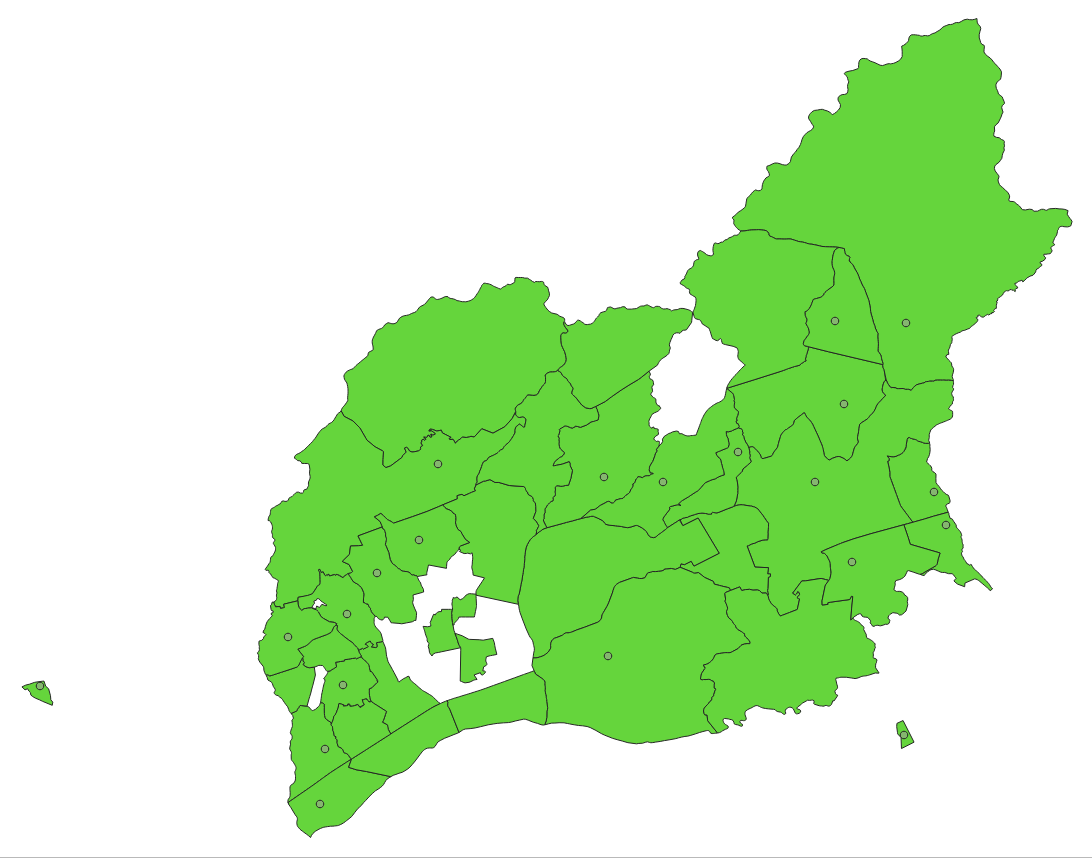
\includegraphics[height=0.75\textwidth]{images/4_materiais/gis/Guarulhos_SHAPE_QGIS.png}
        \label{fig:GRU_shapefile}
    \end{subfigure}
    \begin{subfigure}{0.49\textwidth}
        \subcaption{Após as correções}
        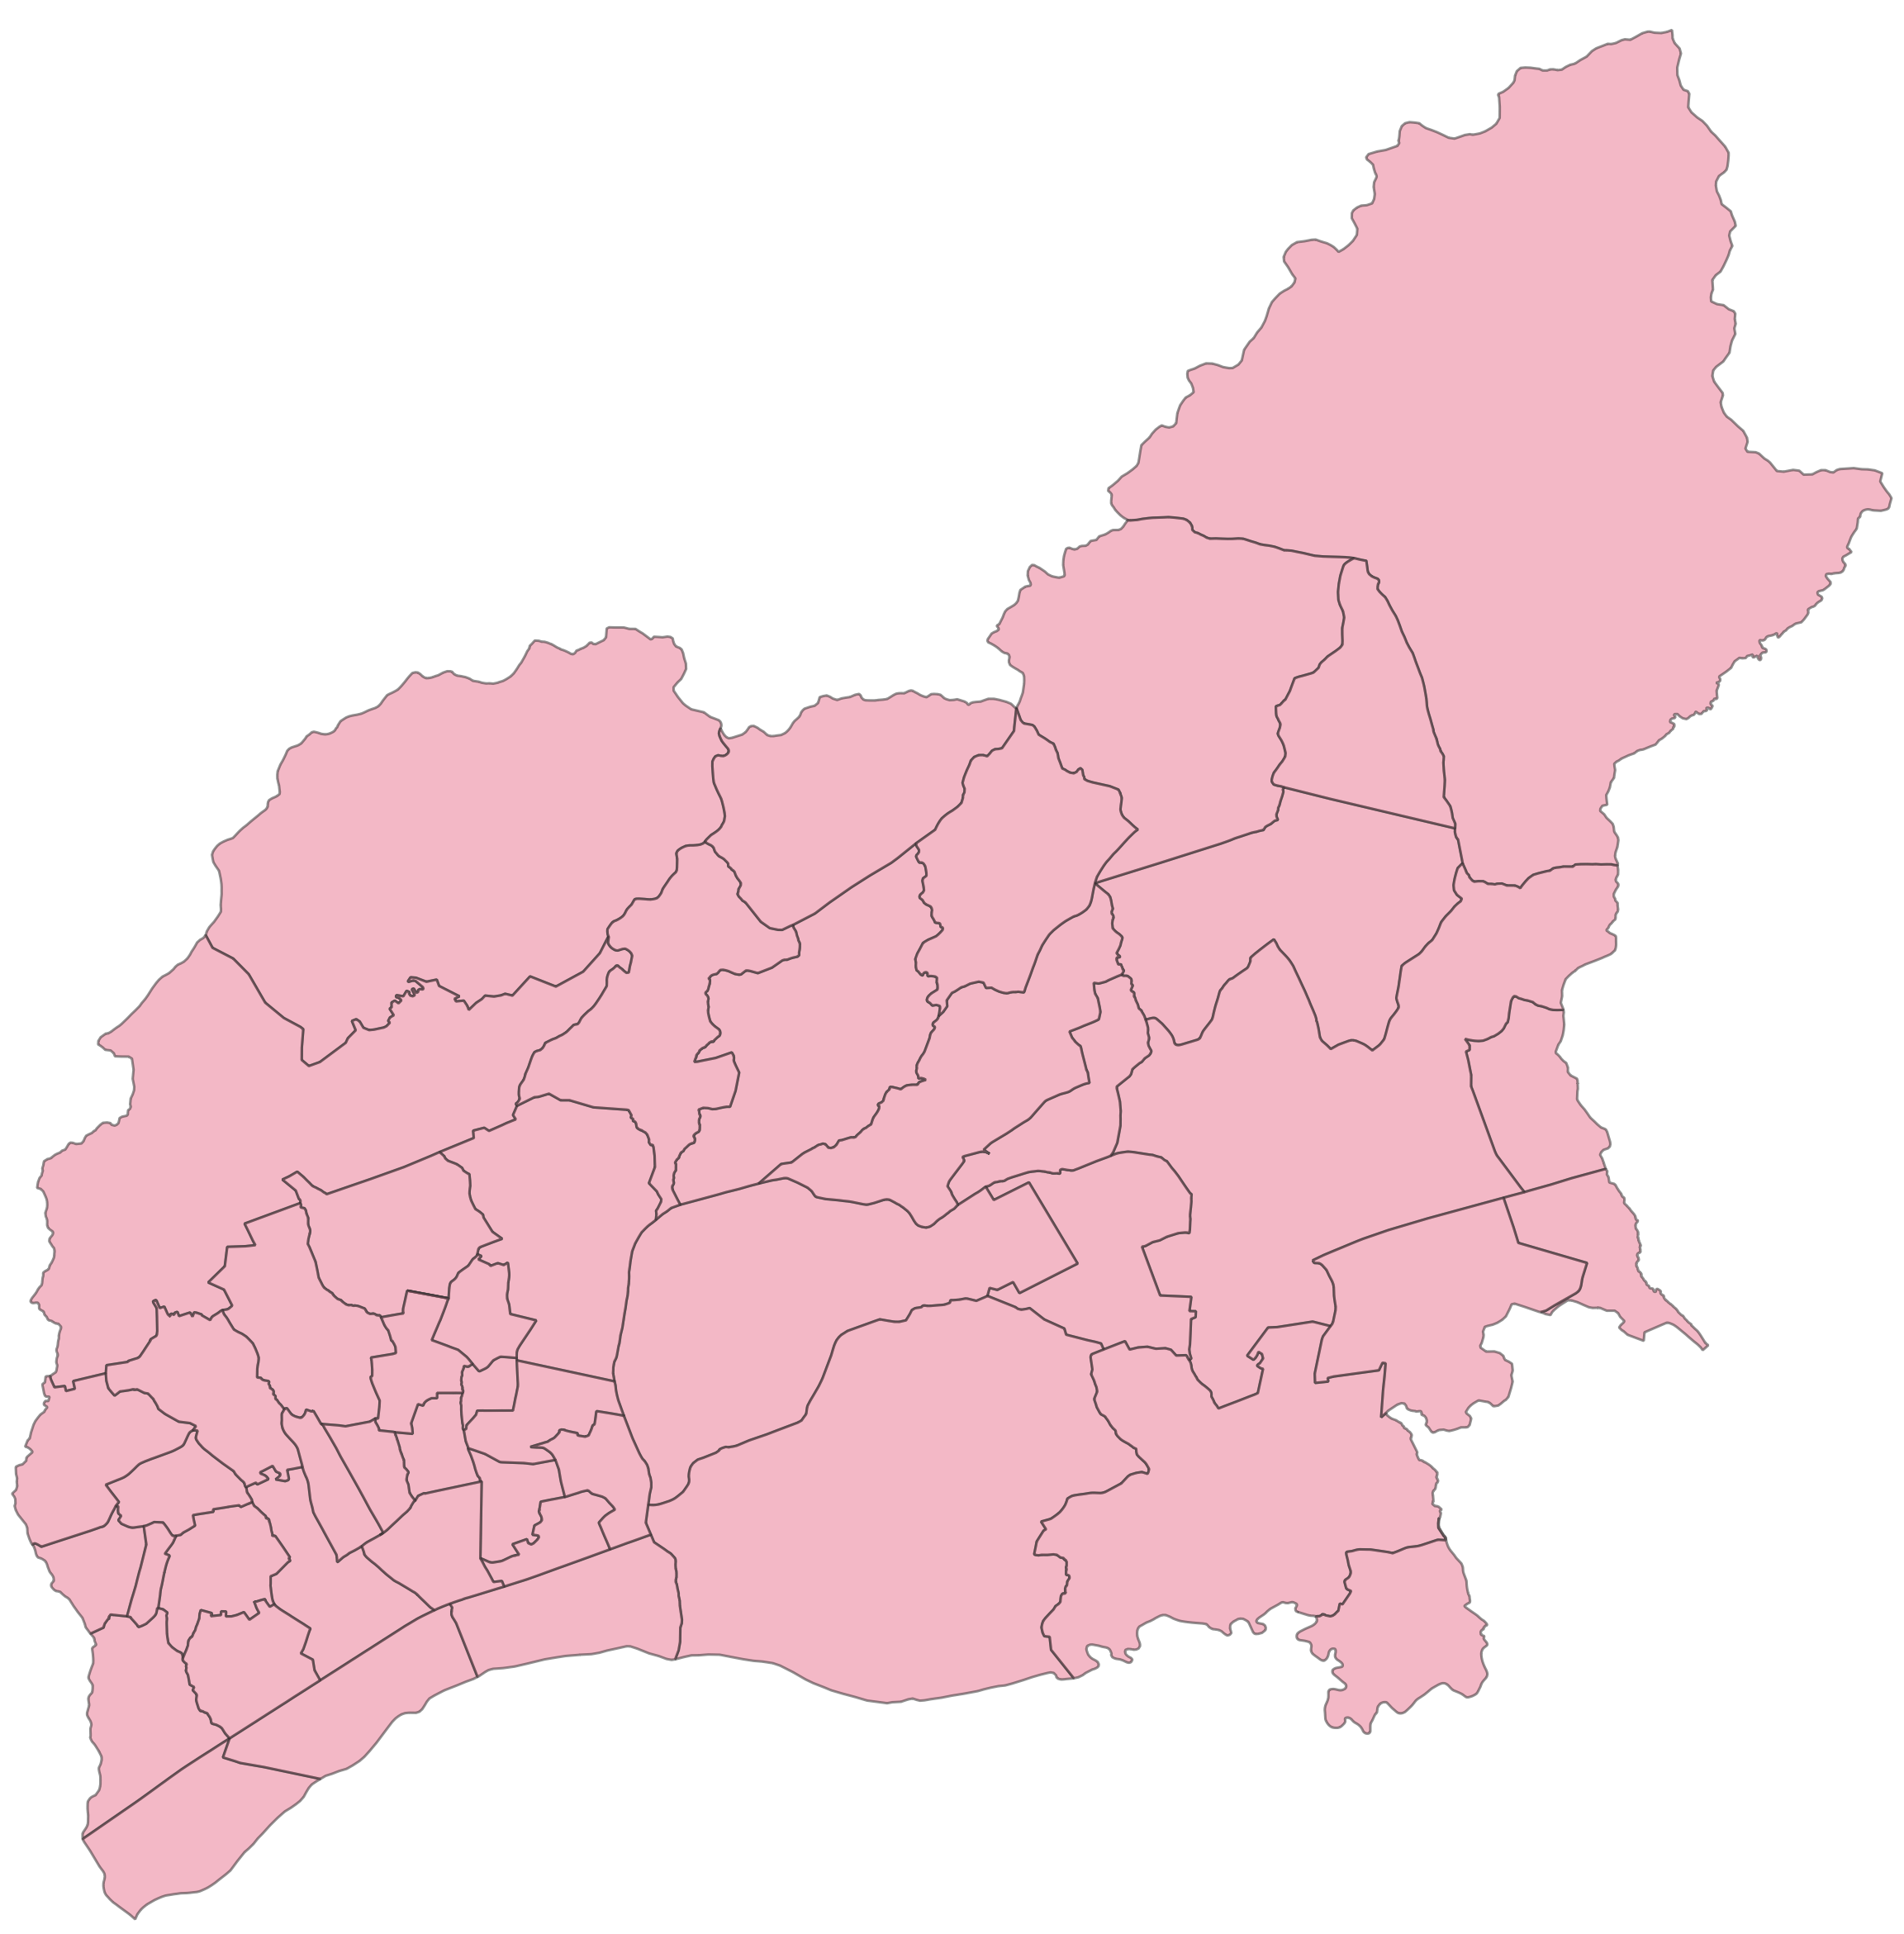
\includegraphics[height=0.75\textwidth]{images/4_materiais/gis/BairrosGuarulhosNovo.png}
        \label{fig:GRU_shapefile_QGIS}
    \end{subfigure}
    \centering
    \caption*{Fonte: Produzido pelos autores Fernandes \& Alves}
\end{figure}

A tabela \ref{tab:Bairros_shapefile}, disponível na seção \ref{sec:AppGIS}, traz o resumo do que se tem de informação deste arquivo \textit{shapefile} inicial que, no caso, são apenas o nome de cada bairro e sua área.

%%%%%%%%%%%%%%%%%%%%%%%%%%%%%%%%%%%%%%%%%%%%%%%%%%%%%%%%%%%
\subsection{Los Angeles, CA, Estados Unidos} \label{SIG_LA}

Na segunda parte do trabalho, em contraste a Guarulhos, é necessário que se obtenha dados georreferenciados das cinco cidades que compõe a operação amostrada da \textit{Amazon} na base de dados disponibilizada. 
%
Um grande enfoque do trabalho especialmente nas primeiras análises, porém, foi dado ao condado de Los Angeles, situado no Estado da Califórnia (EUA), devido à sua boa representatividade percentual da operação comparada às outras cidades.

Seguindo-se o mesmo procedimento do município de Guarulhos observado no tópico \ref{sec:georef_guarulhos}, buscou-se segregar a cidade em bairros para agrupar os dados da operação. 
%
Para tal, encontrou-se, nos arquivos públicos da Universidade do Sul da Califórnia (USC), um arquivo \textit{shapefile} atualizado dos polígonos que compõem cada bairro do município, como observado em \citeonline{USC2022}.
%
Diferentemente do caso de Guarulhos, o arquivo \textit{shapefile} de Los Angeles é composto por múltiplos bairros que não necessariamente apresentam atividade operacional da \textit{Amazon} e que, em geral, compreendem extensas áreas. 
%
Assim, visando o desempenho computacional de etapas futuras, selecionou-se apenas os polígonos dos bairros que continham, de fato, atividades operacionais da base de dados utilizada. 
%
Assim, resultou-se no polígono apresentado na Figura \ref{fig:bairros_LA}, que representa os bairros do condado de Los Angeles em cor branca (não selecionados) e azul (selecionados).

\begin{figure}[htbp]
    \centering
    \caption{Bairros de Los Angeles selecionados para análise}
    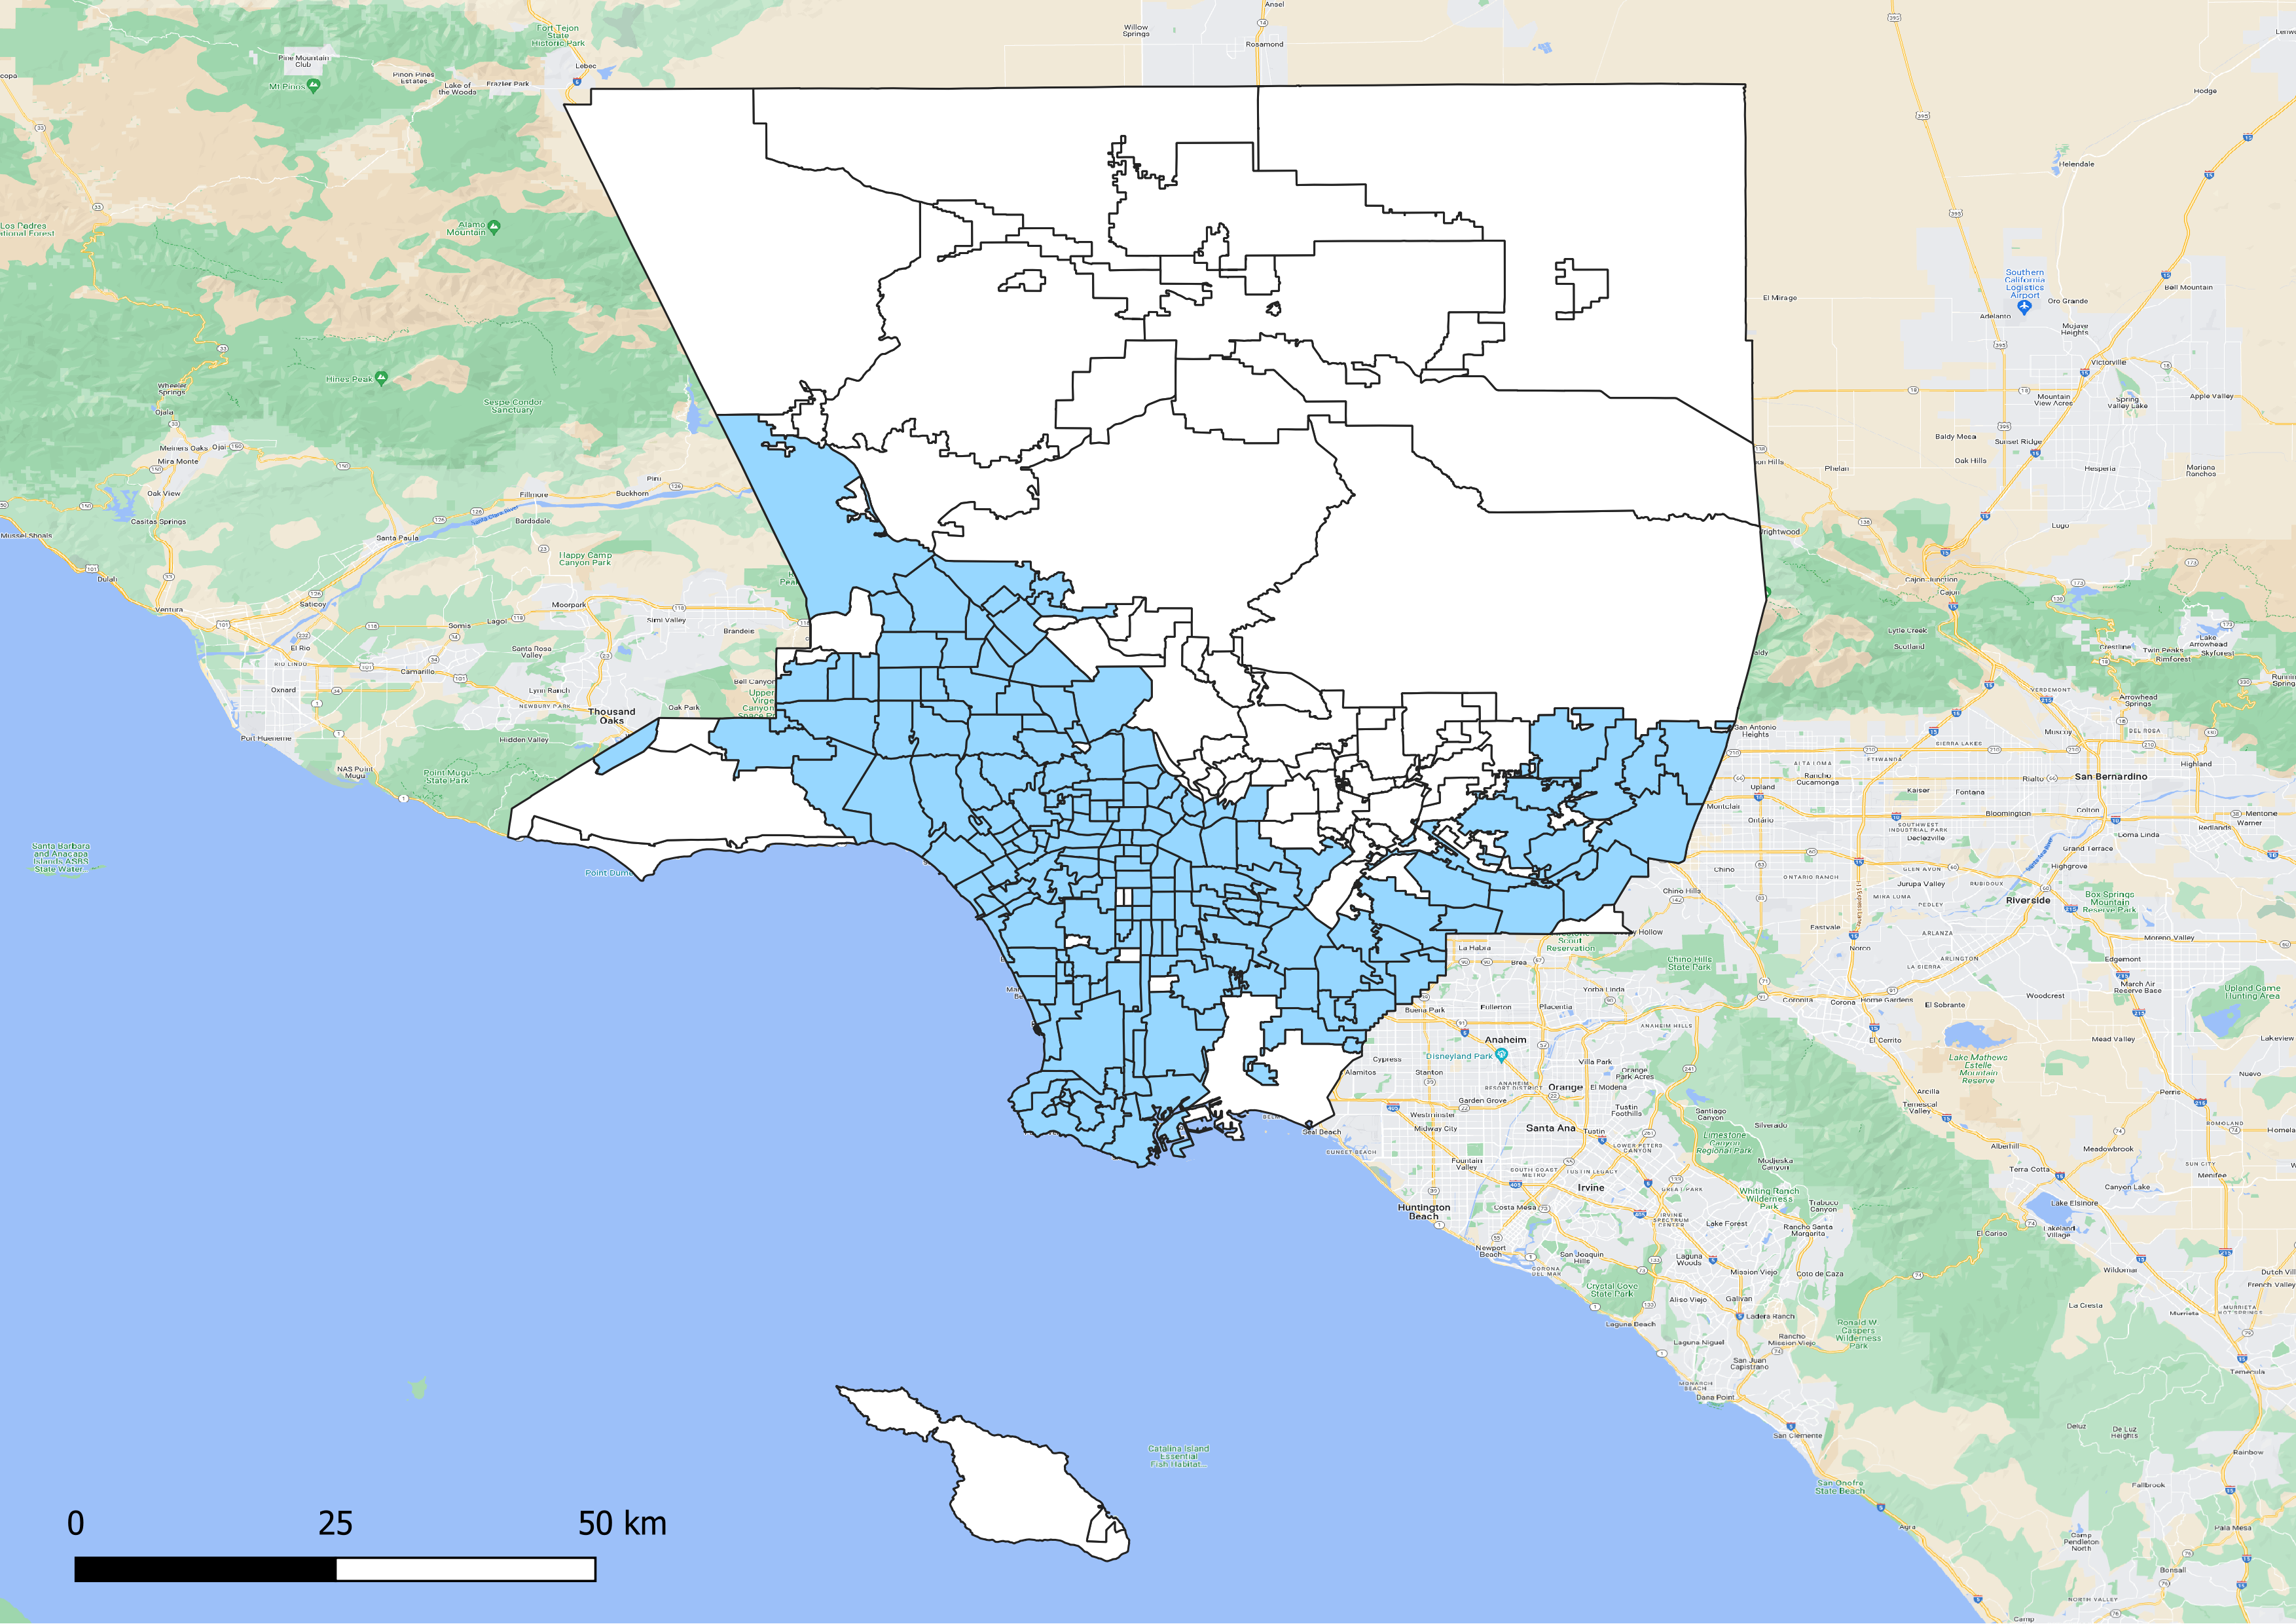
\includegraphics[width=0.8\textwidth]{images/4_materiais/gis/LA_BairrosSelecionados.png}
    \caption*{Fonte: Produzido pelos autores Fernandes \& Alves}
    \label{fig:bairros_LA}
\end{figure}

Vale ressaltar que a peculiaridade de bairros sem operação de entregas resulta do fato de o município de Los Angeles, na região norte, possuir regiões montanhosas e pouco habitadas.
Este fenômeno também está presente no \textit{shapefile} (Figura \ref{fig:GRU_shapefile_QGIS}) da cidade de Guarulhos, sugerindo que, em geral, bairros mais ao centro da cidade geralmente são menores e mais discretizados. 

\subsection{Demais cidades americanas}

Dado que a base de dados operacional da Amazon compõe-se ao longo de cinco grandes regiões metropolitanas nos Estados Unidos: Austin, Boston, Chicago, Los Angeles e Seattle; e, apesar do foco supracitado ao município de Los Angeles, também buscou-se obter dados georreferenciados das outras 4 cidades. 
%
Para tal, repetiu-se o processo citado anteriormente para Los Angeles cidade a cidade, buscando o mapeamento dos bairros das cidades em fontes oficiais, tais como prefeituras, governos estaduais, universidades e institutos. No caso de Austin, Texas, o mapeamento foi obtido através de \citeonline{Austin2022}. Já os bairros de Boston foram obtido em \citeonline{BPDA2020}. No caso de Chicago, a prefeitura disponibilizou os dados em \citeonline{Chicago2022}. E, por fim, os bairros de Seattle foram obtidos em \citeonline{Seattle2021}.
Por fim, obtém-se uma relação de polígonos que descrevem bairro a bairros os municípios das 5 cidades.

%%%%%%%%%%%%%%%%%%%%%%%%%%%%%%%%%%%%%%%%%%%%%%
\section{Geoestatísticas} \label{GeoDa}

Através do \textit{GeoDa}, buscou-se estabelecer procedimentos que permitissem análises geoespaciais de dados, como por exemplo análises referentes à autocorrelação espacial, conforme descritas na seção \ref{sec:autocorrelacaoEsp}.
%
Para que se utilize tal análise, é necessário que os dados estudados sejam organizados numa estrutura de zonas. 
Assim, como supracitado na Seção \ref{sec:dados_de_informacao_geografica}, é possível estruturar a região estudada em bairros.

Em seguida define-se as diferentes variáveis a serem estudadas. 
Como já apresentado no tópico \ref{sec:variaveis_do_problema}, considera-se, ao longo do trabalho, as variáveis Repasse, devolução e NAS, obtendo-se a o valor de cada variável em cada zona e, em sequência, pode-se construir a análise de Moran citada.
%
Tal construção produz um mapa LISA e um gráfico de dispersão para cada variável estudada (percentual de repasses, devoluções e NAS).

Maiores detalhes acerca dos conceitos por trás das ferramentas e teorias utilizadas no GeoDa por ser encontrados na Seção \ref{sec:autocorrelacaoEsp}.

%%%%%%%%%%%%%%%%%%%%%%%%%%%%%%%%%%%%%%%%%%%%%%
\section{Dispersão geográfica das rotas} \label{sec:dispGeoRotas}

Para quantificar a composição geográfica das rotas, optou-se por construir uma nova medida nomeada ``dispersão geográfica da rota''. 
Sua concepção baseia-se na tese de que clientes mais segregados do resto dos clientes de uma mesma rota podem apresentar um comportamento diferente dos demais. 
Tal tese é estruturada na ideia de que a equipe de entregas da rota em questão pode oferecer um tratamento particular a PDEs localizados à parte da maioria dos PDEs de tal rota.

Assim, para cada rota, calcula-se a distância de todos os PDEs que a compõe entre si. 
Em sequência, calcula-se a média das distância para cada PDE, em cada rota.
Desta forma, é possível mensurar o quão longe cada PDE está dos outros PDEs da mesma rota.
Posteriormente, assume-se que há uma distribuição normal de probabilidade dessas distâncias médias em cada rota, para que se possa identificar quais PDEs estão mais à deriva da distribuição espacial e, por consequência, estão localizados na região da ``cauda'' da distribuição normal. 
Para tal, utilizou-se a normalização da variável distância à Distribuição Normal Padronizada (Z). 

Tal divisão pode ser exemplificada nas Figuras \ref{fig:AMBEV_Compac_1}, \ref{fig:AMBEV_Compac_2} e \ref{fig:AMBEV_Compac_3}, advindas do teste da metodologia na base de dados da empresa de bebidas.
Nelas, observa-se a composição de PDEs de duas rotas distintas.
Os PDEs são coloridos de forma a identificar, no corte de 95\% de significância, os que são considerados marginais (vermelho) e os que não são (azul). 

\begin{figure}[H]
    \centering
     \caption{Exemplos de rotas segregadas entre marginais e não-marginais.}
     \begin{subfigure}{.3\textwidth}
         \centering
         \caption{Exemplo 1.}
         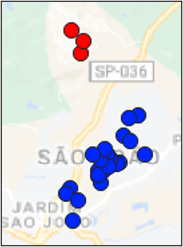
\includegraphics[height=1.2\textwidth]{images/4_materiais/compactacao/CompactacaoExemplo1.png}
         \label{fig:AMBEV_Compac_1}
     \end{subfigure}
     \begin{subfigure}{.3\textwidth}
       \centering
       \caption{Exemplo 2.}
       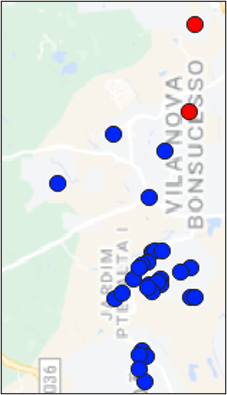
\includegraphics[height=1.2\textwidth]{images/4_materiais/compactacao/CompactacaoExemplo2.png}
       \label{fig:AMBEV_Compac_2}
     \end{subfigure}
     \begin{subfigure}{.3\textwidth}
       \centering
       \caption{Exemplo 3.}
       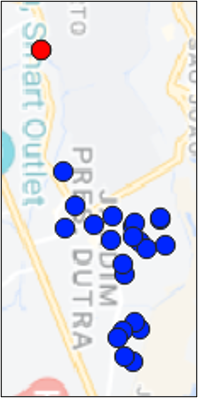
\includegraphics[height=1.2\textwidth]{images/4_materiais/compactacao/CompactacaoExemplo3.png}
       \label{fig:AMBEV_Compac_3}
     \end{subfigure}
     \caption*{\ Fonte: Produzido pelos autores Fernandes \& Alves}
     % \small\textsuperscript{} Observação: As figuras foram rotacionadas para melhor visualização.
 \end{figure}

\section{Criação da biblioteca \textit{Last-Mile-Routing-Analyzer}} \label{BibLMRA}

Para realizar os dois estudos de casos de forma eficiente e replicável, foi desenvolvida e publicada uma biblioteca de código aberto escrita em linguagem \textit{Python}, nomeada \textit{lmr\_analyzer}.
%
Tal biblioteca consolida uma série de rotinas desenvolvidas durante o trabalho em prol de se obter conhecimentos relevantes a partir das bases de dados e informações geográficas disponibilizadas.
%
Todos os códigos estão disponíveis e documentados publicamente na plataforma Github (\citeauthoronline{guilherme_fernandes_alves_2022_6792977}, \citeyear{guilherme_fernandes_alves_2022_6792977}).
%
Os termos pacote, módulo e biblioteca são utilizados como sinônimos neste trabalho. 
Alguns conceitos de programação orientada a objetos (\citeauthoronline{cox1986object}, \citeyear{cox1986object}) serão empregados ao longo do texto, tais como classes, métodos, atributos, etc.. 

A estrutura básica do pacote \textit{lmr\_analyzer} pode ser vista na Figura \ref{fig:UMLPython}, de onde se obtém que as principais classes desenvolvidas são: \textit{package}, \textit{stop}, \textit{route}, \textit{distanceMatrix}, \textit{analysis} e \textit{geometry}, além de um módulo \textit{amzSerializer} específico para tratamento da base de dados da Amazon.
%
A classe \textit{package} é a primeira das classes básicas da \textit{lmr\_analyzer}, ela concentra as informações de dimensão e status de cada pacote a ser entregue, i.e. se ele se trata de um pacote entregue, devolvido ou a ser entregue.
%
A classe \textit{stop} armazena informações relativas aos diferentes pontos de interesse, sejam eles PDEs ou CDs.
%
Para ser inicializada, a classe \textit{stop} recebe um ou mais objetos da classe \textit{package}, além de informações como a latitude e longitude do local e os horários de funcionamento.
%
Em seguida, um conjunto de objetos da classe \textit{stop} é utilizado para definir um objeto da classe \textit{route} que, para que seja inicializado, também necessita de um objeto \textit{vehicle} e do horário de início da rota.
%
Finalmente, a classe \textit{analysis} realiza operações com base nos dados armazenados em um conjunto de \textit{routes} e um objeto \textit{geometry} que descreve as informações espaciais disponíveis.
%
Adicionalmente, o submódulo \textit{utils} contém funções e métodos genéricos que podem ser reutilizadas pelas demais classes.
%
Através dessa estrutura de dados é possível tirar proveito, simultaneamente, das informações espacial e das bases de dados fornecidas. 

\begin{figure}[H]
    \centering
    \caption{Diagrama UML da biblioteca \textit{lmr\_analyzer}}
    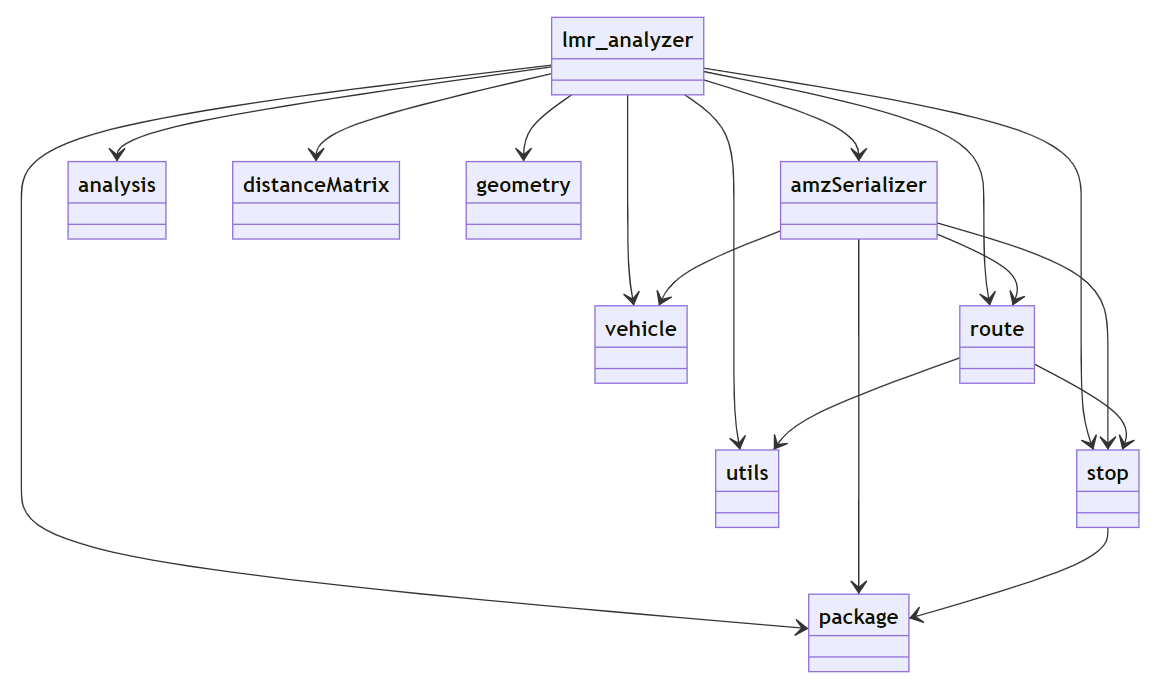
\includegraphics[width=0.6\textwidth]{images/4_materiais/lmr_analyzer/lmr_analyzer_UML.png}
    \caption*{Fonte: Produzido pelos autores Fernandes \& Alves}
    \label{fig:UMLPython}
\end{figure}

Dentre as funcionalidades disponíveis na \textit{lmr\_analyzer} estão a capacidade de processar e armazenar os dados de entregas última milha em objetos de diferentes classes, obtenção de distancias sob diferentes modos (euclidiana, distância veicular, etc.), cálculo de fator de circuito, análise quantitativa de malhas viárias incluindo distribuição da orientação de vias e, finalmente, a importação e exportação de arquivos \textit{shapefiles} contendo as informações analisadas.
%
Além disso, devido à flexibilidade da linguagem de programação \textit{Python}, é possível integrar os resultados e dados de entrada da biblioteca com as demais ferramentas do trabalho.
%
Na prática, o que se estabelece é um procedimento - \textit{framework} - que facilita a transformação de dados brutos em resultados tratados que podem ser visualizados em diversos ambientes, como por exemplo o \textit{QGIS}.
%
A seguir, apresenta-se detalhadamente cada uma das funcionalidades mencionadas. 
Contudo, destaca-se que um maior detalhamento de cada etapa está presente na seção de apêndice \ref{sec:AppCodes}.

\subsection{Fluxo de trabalho}

Explorando o tópico de flexibilidade como uma das vantagens da biblioteca criada, podemos descrever qual a usabilidade esperada ao se trabalhar com a mesma.
%
O fluxo de trabalho padrão estabelecido através da biblioteca acompanha o modelo descrito na Figura \ref{fig:flowchart}. 
%
Podemos notar que o usuário precisa primeiro definir o conjunto de dados relativos às rotas a serem analisadas.
%
Duas sequências podem ser atribuídas nesta etapa, com auxílio da classe \textit{route}, sendo elas a sequência programada e a sequencia realmente executada.
Essas duas sequências são completamente independentes, e o \textit{software} não requer que ambas sejam inseridas simultaneamente para que se obtenha os resultados disponíveis.
%
Em outras palavras, caso o usuário disponha apenas de informações relativas a rotas programadas, sem ter dados de como as rotas realmente se saíram na prática, poderá utilizar a ferramenta para realizar os estudos que serão indicados ao longo deste trabalho.
O caminho contrário também é possível.

Já quanto às informações espaciais, estas em geral representam dados não muito diferentes dos que foram apresentados na seção \ref{sec:dados_de_informacao_geografica}.
%
Em suma, um arquivo \textit{\textit{shapefile}} que contenha uma descrição espacial da cidade a ser analisada pode ser utilizado como dado de entrada.
%
Para as análises que serão feitas neste trabalho, escolheu-se uma discretização da cidade através dos contornos dos bairros.

\begin{figure}[H]
    \centering
    \caption{Fluxo de dados para utilização da biblioteca \textit{lmr\_analyzer}}
    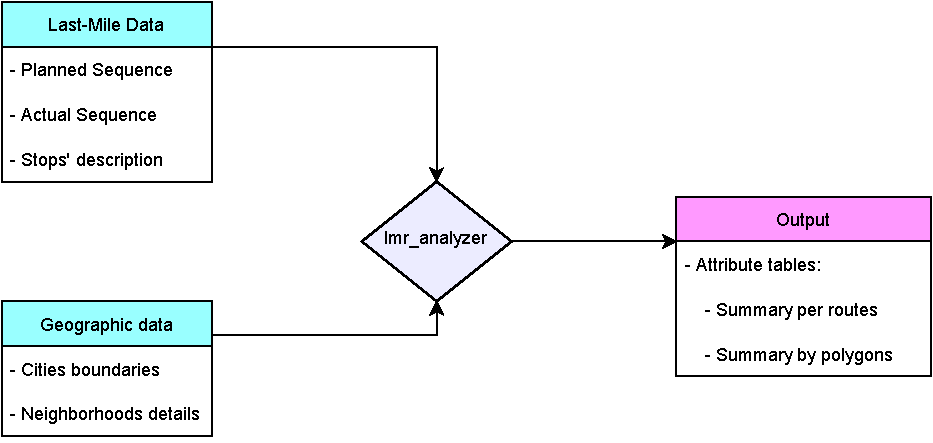
\includegraphics[width=0.8\textwidth]{images/4_materiais/lmr_analyzer/flowchart.pdf}
    \caption*{Fonte: Produzido pelos autores Fernandes \& Alves}
    \label{fig:flowchart}
\end{figure}


\subsection{Cálculo do fator de circuito através do \textit{Google Maps API}} \label{sec:codigosmaps}

Inicialmente foi utilizada a plataforma \textit{Google Maps} para cálculo das distâncias reais percorridas entre diferentes PDEs e o CD, para então compará-las com a distância euclidiana por meio da medida de fator de circuito introduzida no capítulo \ref{sec:revis_biblio}. 
%
O método utilizado para se obter as distâncias do \textit{Google Maps} através da \textit{lmr\_analyzer} estão descritos na subseção \ref{sec:codigosmaps}, no capítulo de apêndice \ref{sec:AppCodes}.
%
A partir da Figura \ref{fig:rota_LA_CF} podemos visualizar um exemplo comum de rotas que serão estudadas.
No caso em questão, as distâncias a serem calculadas estão representadas pelas linhas cheias, que correspondem com a sequência real que a rota apresentou.

\begin{figure}[htbp]
     \caption{Exemplo de rota na cidade de Los Angeles}
     \begin{subfigure}{.49\textwidth}
         \centering
         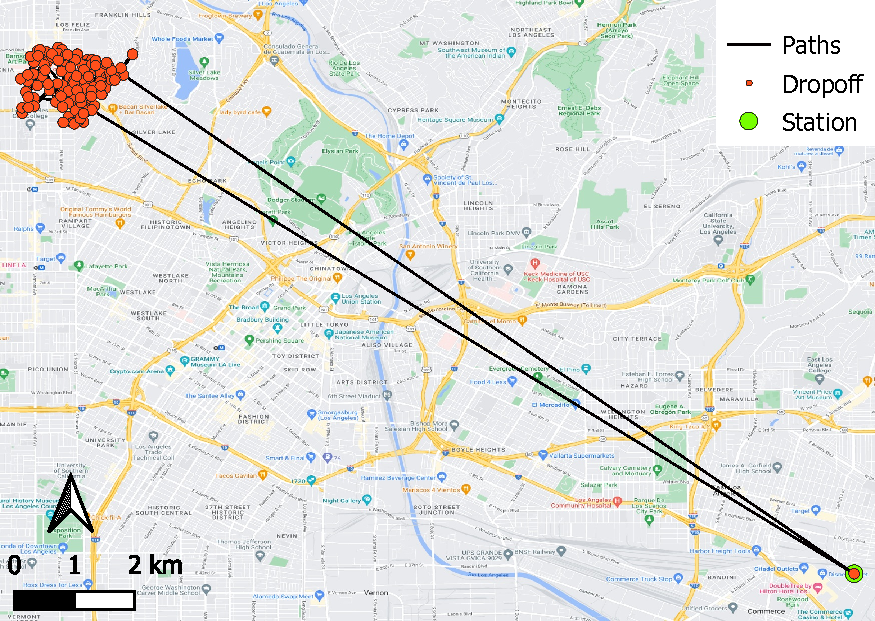
\includegraphics[height=0.63\textwidth]{images/4_materiais/lmr_analyzer/cf_LA_example_zoom.pdf}
     \end{subfigure}
     \begin{subfigure}{.49\textwidth}
       \centering
       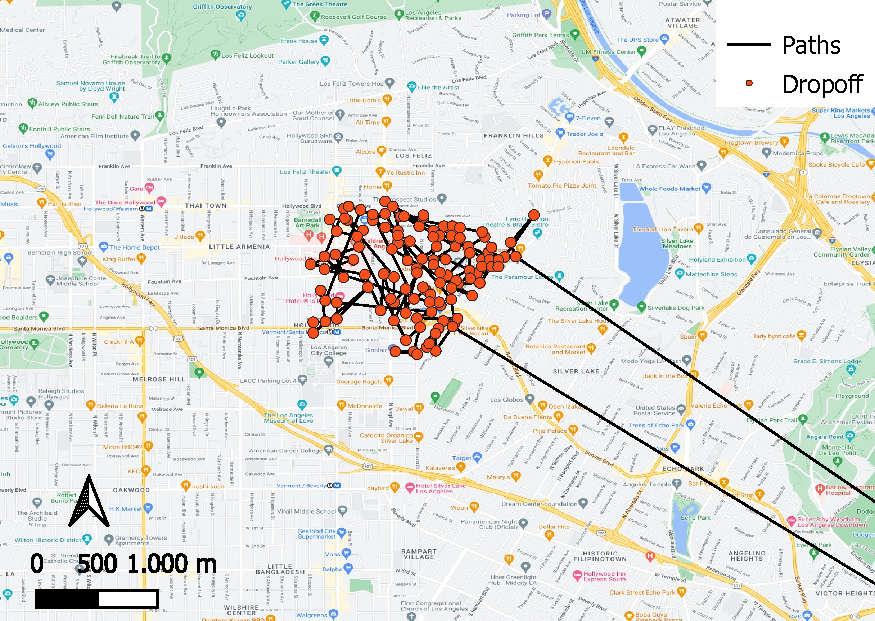
\includegraphics[height=0.63\textwidth]{images/4_materiais/lmr_analyzer/cf_LA_example_zoom_in.pdf}
     \end{subfigure}
     \caption*{\ Fonte: Produzido pelos autores Fernandes \& Alves}
     \label{fig:rota_LA_CF}
 \end{figure} % Repasses

Ademais, para complementar a análise também é preciso estimar a distância em linha reta entre os diferentes pontos.
%
Será adotada a aproximação de que as distâncias entre os pontos são sempre suficientemente pequenas, assim permitindo utilizar a fórmula de \textit{Haversine} (\citeauthoronline{robusto1957cosine}, \citeyear{robusto1957cosine}) para se obter a distância de grande círculo e então aproximá-la como sendo a distância euclidiana entre os pontos.
%
Como essas distâncias não passam de duas centenas de quilômetros, tal hipótese pode ser adotada sem grandes problemas.

Tendo posse da distância em linha reta e das distâncias veiculares (\textit{driving distances}), é possível calcular o fator de circuito entre os diferentes trechos de cada rota.
Ademais, calcula-se também o fator de circuito global de cada rota de acordo com a Equação \ref{eq:Cf_TOTAL}.

\begin{equation} \label{eq:Cf_TOTAL}
    CF_{total} = \frac{total\;driving\;distance}{total\;euclidean\;distance}
\end{equation}

Sendo assim, os atributos que serão calculados nesta etapa, portanto, são: 
\begin{enumerate}
    \item \textbf{planned\_driving\_distances}: Vetor contendo as distâncias reais percorridas entre cada trecho da rota. Este vetor contém $n$ elementos, sendo $n$ o número de entregas. Considera-se que, ao realizar a última entrega, o veículo retorna para o ponto de origem (geralmente o CD). Cada elemento do vetor representa a distância do PDE que está naquela posição até o PDE subsequente. 
    \item \textbf{planned\_euclidean\_distances}: Vetor análogo ao descrito imediatamente acima, porém desta vez contendo as distâncias em linha reta entre os diferentes PDEs.
    \item \textbf{planned\_circuity\_factors}: Representa o fator de circuito entre cada um dos trechos. É calculado simplesmente dividindo-se os dois vetores anteriores.
    \item \textbf{avg\_planned\_circuity\_factor}: Representa a média do fator de circuito dos trechos, os seja, a média do vetor planned\_circuity\_factors.
    \item \textbf{max\_planned\_circuity\_factor}: Valor máximo do fator de circuito da rota.
    \item \textbf{min\_planned\_circuity\_factor}: Valor mínimo do fator de circuito da rota.
    \item \textbf{total\_planned\_driving\_distance}: Soma de todas as distâncias percorridas na rota.
    \item \textbf{total\_planned\_euclidean\_distance}: Soma de todas as distâncias euclidianas.
    \item \textbf{total\_planned\_circuity\_factor}: Divisão entre a soma de distâncias percorridas e a soma de distâncias euclidianas. Representa a medida $CF_{total}$, tal como apresentada na Equação \ref{eq:Cf_TOTAL}.
\end{enumerate}

Estes atributos se repetem, da mesma forma, para a sequência real executada. 
As operações básicas entre os diferentes vetores (soma, divisão, etc.) são facilitadas através de programas escritos linguagem C e contidos na biblioteca \textit{numpy} para \textit{Python} (\citeauthoronline{harris2020array}, \citeyear{harris2020array}).

%%%%%%%%%%%%%%%%%%%%%%%%%%%%%%%%%%%%%%%%%%%%%%%%%%%%%%%%%%%%%%%%%
\subsection{\textit{OSRM} como alternativa ao \textit{Google Maps API}}

Um problema enfrentado na abordagem anterior é a limitação de número de consultas gratuitas permitidas pela \textit{API} do \textit{Google Maps}, o que exigiria investimento financeiro para finalizar a pesquisa (ou seja, para para utilizar a ferramenta acima de um certo limite).
Sendo assim, buscou-se como alternativa a plataforma \textit{Open Source Routing Machine} (\citeauthoronline{luxen2011real}, \citeyear{luxen2011real}), que permite calcular todas as possíveis rotas entre dois ou mais pontos diferentes e, assim, escolher a rota de menor caminho ou tempo.
%
A ferramenta recebe como dados de entrada as coordenadas geodésicas dos pontos a serem analisados e, como resultado, entrega a distância a ser percorrida, o tempo previsto de deslocamento e também o caminho a ser percorrido.
Para o trabalho em questão, apenas a distância será utilizada, aliviando a quantidade de dados a serem armazenados.
Uma descrição mais detalhada do método empregado encontra-se disponível na seção de apêndices \ref{sec:AppCodes}.

De toda forma, ambas as metodologias (\textit{googlemaps} e \textit{OSRM}) permanecem disponíveis na biblioteca \textit{lmr\_analyzer} e, dependendo da aplicação, o usuário final poderá escolher qual a mais adequada.
%
Para o desenvolvimento deste trabalho, algumas das distâncias foram calculadas utilizado o método do \textit{Google Maps}, uma vez que a plataforma oferece um período de utilização livre de cobranças (\textit{free trail}).
Uma vez encerrado este período, passou-se a utilizar a plataforma exclusivamente a plataforma \textit{open-source}.

%%%%%%%%%%%%%%%%%%%%%%%%%%%%%%%%%%%%%%%%%%%%%%%%%%%%%%%%%%%%%%%
\subsection{Modelo para avaliação topológica de malhas viárias}

Uma vez definidos os valores da medida de fator de circuito para cada trecho de rota, bem como para a rota como um todo, foi possível explorar a vertente geoespacial da análise, que neste caso é representada pela malha viária da cidade.
%
Para tanto, foi utilizada a biblioteca \textit{OSMnx} (\citeauthoronline{BOEING2017126}, \citeyear{BOEING2017126}) que, conforme descrito na seção \ref{sec:revis_biblio}, permite modelar, analisar e visualizar a estrutura de malhas viárias tomando como base dados disponíveis na plataforma do \textit{OpenStreetMap}.
%
A \textit{OSMnx} faz uso da biblioteca \textit{geopandas} (\citeauthoronline{jordahl2014geopandas}, \citeyear{jordahl2014geopandas}) para facilitar o tratamento de dados espaciais, assim, este trabalho também fez uso de tal biblioteca. 
O que foi realizado dentro do pacote \textit{lmr\_analyzer}, através de um arquivo em formato \textit{shapefile} que descreva o contorno de cada bairro da cidade, iterar sobre cada polígono e criar um grafo (\textit{graph}) contendo arcos e nós que representem a malha viária do bairro em questão.
A Figura \ref{fig:graphs_gru_example} apresenta um exemplo de alguns dos grafos gerados para a cidade de Guarulhos, onde os arcos representam segmentos de vias e os nós representam intersecções entre arcos ou extremidades de arcos.

\begin{figure}[htb]
    \centering
    \caption{Exemplo de grafo gerado com o \textit{osmnx} para o bairro de Cumbica em Guarulhos, SP}
        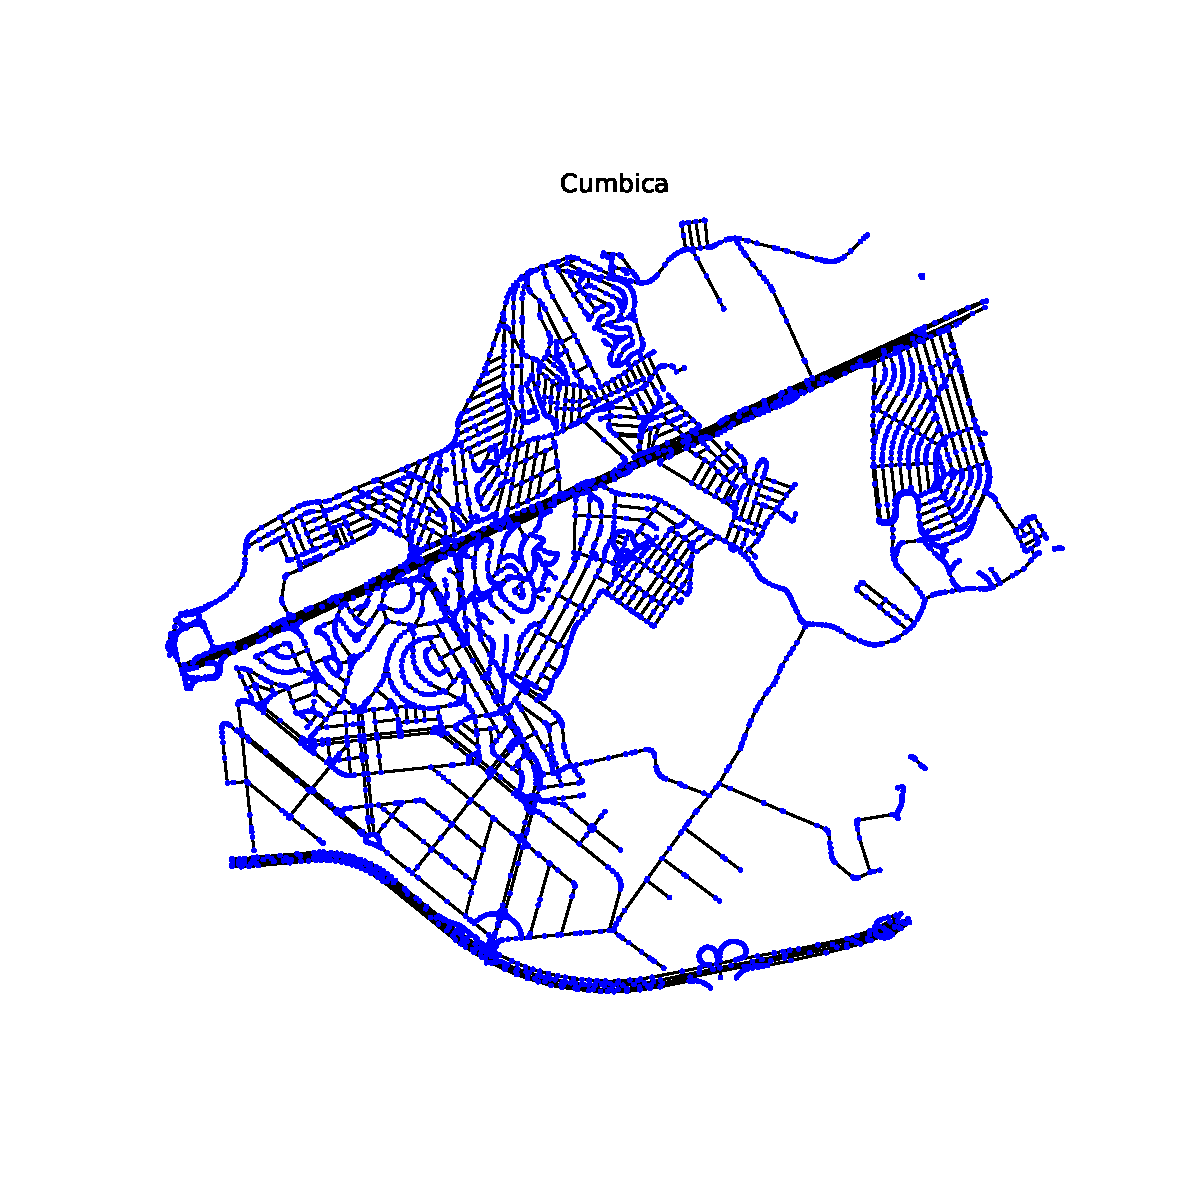
\includegraphics[width=0.6\linewidth]{images/4_materiais/lmr_analyzer/graph_Cumbica.pdf}
    \caption*{\ Fonte: Produzido pelos autores Fernandes \& Alves}
    \label{fig:graphs_gru_example}
\end{figure}

O conjunto de grafos relativos aos bairros da cidade foram armazenados como um dicionário pelo objeto da classe \textit{geometry}.
Assim, foi possível facilmente filtrar, selecionar e/ou alterar os grafos de cada cidade.
Em seguida, foi utilizado o método \textit{osmnx.stats.basic\_stats} para gerar as primeiras estatísticas e parâmetros relativos à malha analisada.
Esse método, presente na \textit{OSMnx}, se apoia principalmente na biblioteca \textit{networkx} (\citeauthoronline{hagberg2008exploring}, \citeyear{hagberg2008exploring}), que é focada justamente em análise de estruturas de rede.
%
As variáveis que foram calculadas nesta etapa estão descritas a seguir:
\begin{itemize}
    % Just copy and paste from here: https://osmnx.readthedocs.io/en/stable/osmnx.html?highlight=stats#osmnx.stats.basic_stats
    \item \textbf{circuity\_avg}: é a soma dos comprimentos dos arcos dividida pela soma das distâncias em linha reta entre as extremidades dos arcos. Valores próximos a 1 podem ser reflexo de uma malha bem discretizada, enquanto que valores muito diferentes de 1 podem indicar presença excessiva arcos curvilíneos. Apesar do nome, esta variável não tem relação com a medida de fator de circuito utilizada em outras partes do texto.
    \item \textbf{intersection\_count}: Número de intersecções presentes no grafo.
    \item \textbf{intersection\_density\_km}: Número de intersecções dividido pela área do polígono
    \item \textbf{edge\_length\_total}: Comprimento total de arcos presentes no grafo
    \item \textbf{edge\_density\_km}: edge\_length\_total dividido pela área do polígono
    \item \textbf{edge\_length\_avg}: edge\_length\_total dividido pelo comprimento total de arcos
    \item \textbf{k\_avg} - Média de arcos conectados em cada nó (\textit{node degree}).
    \item \textbf{m}: número de arcos
    \item \textbf{n}: número de nós
    \item \textbf{node\_density\_km}: n dividido pela área do polígono
    \item \textbf{self\_loop\_proportion}: Porcentagem de arcos que são do tipo \textit{self-loop} em um grafo, ou seja, arcos que estão conectados a um único nó. Um número muito alto indicaria que o grafo analisado não é suficientemente discretizado.
    \item \textbf{street\_density\_km}: street\_length\_total dividido pela área do polígono
    \item \textbf{street\_length\_avg}: street\_length\_total dividido por street\_segment\_count
    \item \textbf{street\_length\_total}: Comprimento total de vias, em geral obtendo valores bastante similares ao comprimento total de arcos.
    \item \textbf{street\_segment\_count}: Contagem de segmentos de vias
    \item \textbf{streets\_per\_node\_counts}: Contagem do número de segmentos de vias.
    \item \textbf{streets\_per\_node\_avg}: Número de seguimentos de vias dividido pelo total de arcos.  
    \item \textbf{streets\_per\_node\_proportions}: A proporção de nós que possuem \textit{n} vias conectadas a si, sendo \textit{n} um inteiro que varia de 1 até infinito.
\end{itemize}

É possível notar que estas medidas muitas das vezes se confundem ou entregam valores redundantes. 
Não obstante, cada uma das medidas é utilizada, na prática, para um propósito diferente.
Sendo assim, convém simplificar e categorizar as medidas utilizadas, conforme apresentada na tabela \ref{tab:metrics_res}, de modo que apenas dez das variáveis apresentadas nesta seção sejam realmente utilizadas durante o trabalho, sendo elas duas voltadas à qualidade da malha gerada e oito voltadas às dimensões gerais da malha.

\begin{table}[htb]
    \singlespacing
    \centering
    \caption{Classificação das medidas geradas para cada um dos grafos}
    \label{tab:metrics_res}
    \begin{tabular}{lcc}
    \hline
    \rowcolor[HTML]{CCCCCC} 
    \multicolumn{1}{|c|}{\cellcolor[HTML]{CCCCCC}\textbf{Quality metrics}} &
      \multicolumn{1}{c|}{\cellcolor[HTML]{CCCCCC}\textbf{Dimension metrics}} &
      \multicolumn{1}{c|}{\cellcolor[HTML]{CCCCCC}\textbf{Redundant metrics}} \\ \hline
    \multicolumn{1}{|c|}{circuity\_avg} &
      \multicolumn{1}{c|}{m} &
      \multicolumn{1}{c|}{\cellcolor[HTML]{F4CCCC}street\_density\_km} \\
    \multicolumn{1}{|c|}{self\_loop\_proportion} &
      \multicolumn{1}{c|}{edge\_density\_km} &
      \multicolumn{1}{c|}{\cellcolor[HTML]{F4CCCC}street\_length\_total} \\
    \multicolumn{1}{|l|}{} &
      \multicolumn{1}{c|}{n} &
      \multicolumn{1}{c|}{\cellcolor[HTML]{F4CCCC}street\_segment\_count} \\
    \multicolumn{1}{|l|}{} &
      \multicolumn{1}{c|}{node\_density\_km} &
      \multicolumn{1}{c|}{\cellcolor[HTML]{F4CCCC}streets\_per\_node\_avg} \\
    \multicolumn{1}{|l|}{} &
      \multicolumn{1}{c|}{intersection\_count} &
      \multicolumn{1}{c|}{\cellcolor[HTML]{F4CCCC}streets\_per\_node\_proportions} \\
    \multicolumn{1}{|l|}{} &
      \multicolumn{1}{c|}{intersection\_density\_km} &
      \multicolumn{1}{l|}{\cellcolor[HTML]{F4CCCC}} \\
    \multicolumn{1}{|l|}{} &
      \multicolumn{1}{c|}{edge\_length\_total} &
      \multicolumn{1}{l|}{\cellcolor[HTML]{F4CCCC}} \\
    \multicolumn{1}{|l|}{} &
      \multicolumn{1}{c|}{edge\_length\_avg} &
      \multicolumn{1}{l|}{\cellcolor[HTML]{F4CCCC}} \\ \hline
    \multicolumn{1}{c}{total: 2} &
      total: 8 &
      total: 5
    \end{tabular}
    \caption*{Fonte: Produzido pelos autores Fernandes \& Alves}
    \onehalfspacing
\end{table}

Ainda dentro do contexto de análise da geometria de malhas viárias, outro modelo aplicado é o de distribuição da orientação de vias.
Conforme apresentado na seção \ref{sec:revis_biblio}, este tema já é bastante explorado por \citeonline{boeing2019urban}, sobretudo quanto ao aspecto de comparação de diferentes malhas viárias a partir dos cálculos que serão apresentados.
Sendo assim, convém simplificar o detalhamento e motivação de alguns dos métodos, mantendo o foco na interpretação dos resultados.

Em primeiro lugar seleciona-se a discretização desejada considerando direções de vias, que variam de 0º a 360º. 
%
Para os casos que serão estudados aqui, selecionou-se 36 intervalos de 10º cada.
%
Em seguida, através da biblioteca \textit{OSMnx} é possível iterar sobre todos os arcos e, para cada um deles, indicar em qual intervalo de direção ele deveria ser alocado.
%
A partir daí realiza-se a contagem do número de arcos que estão dispostos em cada uma das direções e, ao fim, é possível gerar um histograma representando a distribuição das direções dos arcos da malha (grafo) analisada.
%
A Figura \ref{fig:example_histograms} apresenta um exemplo típico de histograma, tanto em projeção linear (esquerda) quanto em projeção polar (direita). 
Apesar de a informação transmitida ser a mesma em ambos os gráficos, em geral opta-se pela projeção polar devido à maior facilidade de visualização.

\begin{figure}[htbp]
    \centering
    \caption{Exemplo de histograma de distribuição da orientação de vias em projeções linear e polar}
    \label{fig:example_histograms}
    \begin{subfigure}{.49\textwidth}
        \raggedleft
        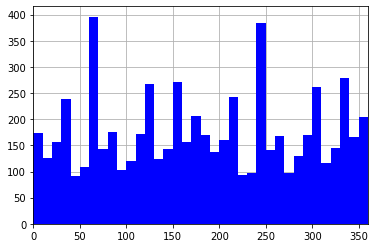
\includegraphics[height=0.55\textwidth]{images/5_emp_bebidas/street_network_analysis/histogram_cumbica.png}
    \end{subfigure}
    \begin{subfigure}{.49\textwidth}
      \raggedright
      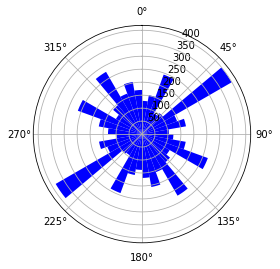
\includegraphics[height=0.55\textwidth]{images/5_emp_bebidas/street_network_analysis/polar_plot_cumbica.png}
    \end{subfigure}
    \caption*{\ Fonte: Produzido pelos autores Fernandes \& Alves}
\end{figure}

\subsection{Aprofundamento das análises de malha viária} \label{sec:aprofund-LMR}

Os métodos disponibilizados pelo pacote \textit{OSMnx} fornecem resultados que enriquecem o valor da pesquisa atual uma vez que é capaz de gerar uma série de estatísticas descritivas sobre diferentes malhas viárias.
Contudo, além da redundância de alguns dos parâmetros, também faz parte das limitações enfrentadas a falta de algumas variáveis mais detalhadas, como seria o caso de variáveis para traduzir em números os histogramas de orientação vistos anteriormente.
Sendo assim, é proposto um conjunto de novos parâmetros para quantificar malhas além dos que estão disponíveis nas configurações padrões do pacote \textit{OSMnx}, parâmetros estes que serão descritos a seguir.

Para começar o processo de quantificar o problema de orientação visto anteriormente, será interessante medir o grau de regularidade da distribuição de orientações apresentada pela malha.
Para tanto, defini-se uma distribuição uniforme de área equivalente à distribuição provinda da malha. 
Essa distribuição significaria o caso hipotético em que as vias estão uniformemente distribuídas em todas as direções possíveis.
Á partir daí é possível comparar a distribuição apresentada pela malha com a distribuição idealizada uniformemente, como ilustrada pela Figura \ref{fig:uniform_histogram}. 
%
A técnica adotada consiste em somar o quadrado da diferença de valores apresentados por essas duas distribuições em cada uma das direções.
Deste modo, cria-se uma medida que ``penaliza'' distorções muito grandes, as quais representariam uma malha onde as vias se concentram sempre em uma única direção específica.

\begin{figure}[htbp]
    \centering
    \caption{Exemplo de comparação entre distribuição real de orientações de vias e hipotética distribuição uniforme equivalente}
    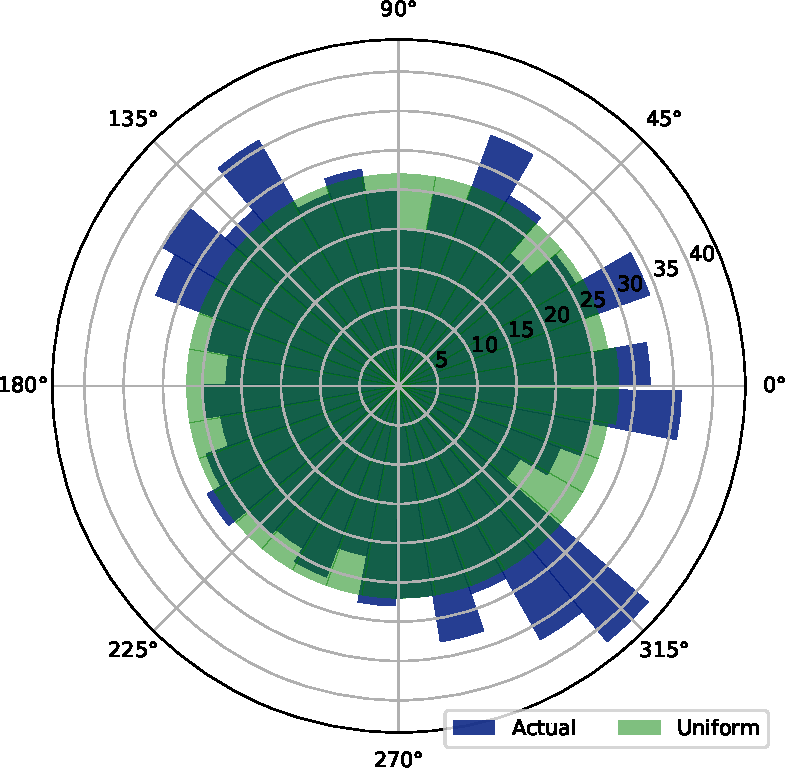
\includegraphics[height=0.45\textwidth]{images/4_materiais/lmr_analyzer/histogram_uniform.pdf}
    \caption*{Fonte: Produzido pelos autores Fernandes \& Alves}
    \label{fig:uniform_histogram}
\end{figure}

Ainda tomando como base o estudo de distribuições, é possível definir os parâmetros de \textit{skew} e \textit{kurtosis}, os quais representam o formato da distribuição analisada.
A variável \textit{skew} quantifica a simetria da distribuição, enquanto que a variável \textit{kurtosis} mede o quanto que a distribuição se aproxima de uma distribuição normal.
Ainda que nos casos estudados muitas vezes a distribuição não será aparente com uma distribuição normal, manter sob observação a variável \textit{kustosis} pode ser relevante para se estabelecer algumas confirmações.

Ademais, defini-se outras variáveis como, por exemplo, a média aritmética das direções e o intervalo de direção dominante.
%
Uma consideração importante sobre estas operações é que, para evitar resultados redundantes em termos de direção, é feita a conversão temporária do intervalo de direções, passando de 0º-360º para 0º-180º.
Este procedimento garante que o modelo não aponte, por exemplo, que a direção dominante e a segunda direção dominante sejam as iguais (porém de sentidos diferentes, e.g. 0º e 180º).
%
As variáveis propostas estão listadas a seguir:

\begin{itemize}
    \item \textit{\textbf{dominant\_direction}}: Intervalo de direção predominante, geralmente aberto limite superior e fechado no inferior. É a moda da distribuição de orientações analisada e pode variar de 0º a 180º.
    \item \textit{\textbf{dominant\_percentage}}: Porcentagem de arcos que pertencem ao intervalo de direções dominante dividido pelo total de arcos.
    \item \textit{\textbf{second\_dominant\_direction}}: Segundo intervalo predominante de direções. Pode variar de 0º a 180º.
    \item \textit{\textbf{second\_dominant\_percentage}}: Porcentagem de arcos que pertencem ao segundo intervalo de direções dominante dividido pelo total de arcos.
    \item \textit{\textbf{mean}} and \textbf{\textit{std}}: Média e desvio padrão, para fins estatísticos apenas. Essas variáveis dificilmente terão valor significativo para representar as direções em questão.
    \item \textit{\textbf{quadratic\_sum\_deviation}}: Soma dos quadrados da diferença entre distribuição apresentada e distribuição uniforme equivalente em cada um dos intervalos. Sempre positivo. Quanto mais próximo de zero, mais a distribuição se aproxima de uma distribuição uniforme, ou seja, a malha tende a não ter nenhuma direção de preferência.
    \item \textit{\textbf{skew}}: Coeficiente de assimetria da distribuição. É calculado como sendo o triplo da diferença entre média e mediana, dividido sobre o desvio padrão da amostra.
    \item \textit{\textbf{kurtosis}}: Momento central de quarta ordem ou média elevada à quarta potência, dividido pela quarta potência do desvio padrão da distribuição. 
\end{itemize}

Ao final, é possível exportar todos os resultados obtidos para o formato apropriado. Em geral, arquivos de extensão \textit{.shp} e \textit{.csv}.

\subsection{Modelos adicionais empregados}

Por fim, é possível descrever alguns modelos extras que também foram importantes para o desenvolvimento e análises do trabalho, como por exemplo a definição do centro de gravidade, ou centroide, para cada rota.
Todos os modelos que serão apresentados estão também disponíveis na biblioteca \textit{lmr\_analyzer} e descritos na seção de apêndice \ref{sec:AppCodes}. 

Embora encontrem-se disponíveis na literatura diversos modelos robustos de como simplificar de forma inteligente uma rota de entregas a um ponto representativo (\citeauthoronline{daganzo1984distance}, \citeyear{daganzo1984distance}), optou-se por adotar simplesmente uma média aritmética das coordenadas geodésicas de todos os PDEs de cada rota, excluindo o(s) CD(s) para que não haja viés.
%
Sendo assim, para uma rota de \textit{n} paradas, em que a primeira quanto a última parada correspondem ao CD, define-se o centroide da rota conforme a equação \ref{eq:CG_rota}.
%
\begin{equation}\label{eq:CG_rota}
    C.G._{route} = \left[lat_{C.G.},\; lon_{C.G.}\right] = \left[\frac{\sum_{i=2}^{n-1} lat_{i}}{n-2},\; \frac{\sum_{i=2}^{n-1} lon_{i}}{n-2}\right]
\end{equation}

Outro dos modelos propostos foi o cálculo da distância entre a rota e o CD.
Estas distâncias podem variar significativamente durante as observações, vista que em geral um único CD é responsável por atender mais de uma cidade. 
%
Novamente, ao buscar metodologias especializadas na literatura, como a proposta por \citeonline{novaes2000continuous}, os autores se depararam com modelos sofisticados e muitas vezes custosos computacionalmente.
%
O que se optou, portanto, foi a simplificação de modo a se computar a distância euclidiana entre o centro de gravidade da rota, descrito pela equação \ref{eq:CG_rota}, e o CD correspondente à rota.
Esta medida já traz uma boa estimativa do quão distantes os PDEs estão do CD. 

Por fim, um dos aspectos relevantes de serem mencionados é com relação à compactação das rotas, que consiste em quantificar a disposição e harmonia espacial das rotas analisadas.
%
Seguindo uma ordem de facilidade, pode-se definir um primeiro indicador como sendo o ``retângulo limite'' (\textit{bounding box}), o qual representa simplesmente o o retângulo de menor área que contenha todos os pontos da rota (excluído o CD).
Para cada \textit{bounding box} é possível calcular a área e a razão de aspecto, de modo a entender o quão dispersos no espaço os pontos das rotas se encontram. 

Ademais, define-se também um método para cálculo de ``polígonos convexos envelopadores'' (\textit{convex hull polygon}).
Um polígono \textit{convex hull} é um polígono convexo e sem buracos que contém todos os pontos desejados porém com menor área possível.
A determinação de tais polígonos foi realizada com auxílio do módulo \textit{spatial} disponível na biblioteca de aplicações científicas para Python denominada \textit{scipy} (\citeauthoronline{2020SciPy-NMeth}, \citeyear{2020SciPy-NMeth}).
A área do polígono \textit{convex hull} será o principal resultado a ser utilizado na análise, porém as coordenadas do polígono também podem ser obtidas, caso necessário.
%
Por outro lado, a evolução natural dos últimos dois métodos é o cálculo do ``retângulo rotacionado de mínima área'' (\textit{minimum rotated rectangule}) que, como o próprio nome diz, representará o retângulo de menor área que contenha todos os pontos da rota, porém sem a limitação anterior (\textit{bounding box}) de o retângulo estar fixado em uma rotação específica.

A titulo de observação, também foram estudados outros formatos não retangulares para estudo de compactação das rotas, como apresentado por \citeonline{gartner1998smallest}, porém a facilidade de implementação configurou-se como um critério importante para seleção do modelo e, desta forma, optou-se pelo método do \textit{minimum rotated rectangule}.

Finalmente, um resumo das medidas que serão calculadas conforme apresentado nesta subseção estão disponíveis logo abaixo:
\begin{itemize}
    \item \textbf{\textit{centroid\_mean}}: Média das coordenadas latitude e longitude dos PDEs presentes na rota.
    \item \textbf{\textit{centroid\_std}}: Desvião padrão das coordenadas latitude e longitude dos PDEs presentes na rota. 
    \item \textbf{\textit{bbox}}: Conjunto de quatro coordenadas definindo o \textit{bounding box} dos pontos da rota, sendo eles: latitude máxima e mínima e longitude máxima e mínima. 
    \item \textbf{\textit{bbox\_area}}: Área do retângulo definido pelo \textit{bounding box}.
    \item \textbf{\textit{bbox\_aspect\_ratio}}: Razão de aspecto do \textit{bounding box}, definida como a divisão do lado maior pelo lado menor.
    \item \textbf{\textit{convex\_hull\_coords}}: Coordenadas do polígono \textit{convex hull} que contém todos os pontos da rota, com exceção do CD.
    \item \textbf{\textit{convex\_hull\_polygon\_area}}: Área do polígono \textit{convex hull}.
    \item \textbf{\textit{mrr}}: Retângulo rotacionado de mínima área e que contenha todos os pontos da rota. É calculado com base no atributo \textit{convex\_hull\_coords}. 
    \item \textbf{\textit{mrr\_area}}: Área do retângulo rotacionado de mínima área.
    \item \textbf{\textit{mrr\_aspect\_ratio}}: A razão de aspecto do retângulo rotacionado de mínima área.
\end{itemize}

Quaisquer outros métodos que venham a ser utilizados para obtenção dos resultados serão explicados pontual e brevemente, porém, finaliza-se este Capítulo tendo sido descritas as metodologias que foram elaboradas ao longo do trabalho com auxílio das referências citar, bem como as hipóteses simplificadoras de cada modelo. 


\chapter{Estudo de caso I: Empresa de Bebidas} \label{sec:EstCasoBebidas}

No presente capítulo serão apresentados os resultados obtidos a partir da base de dados da empresa de bebidas brasileira.
As análises foram divididas a partir da temática geral às quais elas pertencem, considerando uma sequência lógica dos tipos de análises.
Inicialmente, serão apresentadas os valores gerais de Repasse, Devolução e Não Aderência Sequencial (NAS).
Em sequência, na Seção \ref{sec:impactoBebidas}, serão apresentados os impactos que a não aderência operacional tem nas escalas econômica, social e ambiental.
Já na Seção \ref{sec:visita_tecnica}, será apresentada uma descrição acompanhada de considerações gerais acerca da visita técnica realizada a um dos CDs da empresa.

Na Seção \ref{sec:analise_base_dados} busca-se compreender se o comportamento das variáveis-problema em função das características da rota, tais como a posição sequencial do PDE na rota, a frequência de visita do PDE no intervalo estudado, o veículo que realizou a visita, o horário de vista do PDE e o volume entregue ao PDE.
Desta forma, é possível compreender o quão correlatas as variáveis problema são com as características gerais de cada entrega.

Na Seção \ref{sec:distanciaCDBebidas}, em que avalia-se se a distância do PDE ao CD tem algum efeito sobre sua performance nas variáveis-problema.
Ainda considerando-se a posição geográfica dos PDEs, segue-se para a Seção \ref{sec:dispersaoBebidas}, em que considera-se uma relação do PDE para com a sua rota de maneira menos generalizada como realizado nas análises anteriores.
Aqui, busca-se compreender como que o isolamento geográfico de um PDE em relação aos outros PDEs de sua rota pode afetar a ocorrência das variáveis-problema.

A seguir, busca-se avaliar as autocorrelações espaciais das variáveis problema na Seção \ref{sec:geoestatBebidas}.
Tal análise tem como intuito compreender se existe algum padrão espacial na ocorrência das variáveis-problema ou se elas ocorrem do forma aleatória espacialmente. 
As autocorrelações espaciais finalizam as análises que consideram a malha viária. 
Dessa forma, apresenta-se, primeiro, a Seção \ref{sec:AMBEV_FC}, onde avalia-se, em diferentes metodologias, a relação entre o fator de circuito e as variáveis-problema e, em sequência, a Seção \ref{sec:AMBEV_MalhaViaria}, que introduz as variáveis de \citeonline{boeing2019urban} a fim de se avaliar a correlação entre as variáveis-problema e diferentes medidas descritivas da malha viária.
Dessa forma, busca-se compreender o quanto a disposição da malha viária é capaz de explicar os repasses, as devoluções e o NAS.

Por fim, na Seção \ref{sec:relMetricasBebidas}, analisa-se conjuntamente os resultados obtidos nas seções anteriores, de modo a compreender o comportamento de cada variável estudada de forma associada.

Assim, o que se busca com esse capítulo é, em geral, conceber diferentes parâmetros que possam ser associados de modo a se discernir quanto à influência da malha viária nos diferentes aspectos apresentados no restante do trabalho na abrangência da base de dados da empresa de bebidas.

%%%%%%%%%%%%%%%%%%%%%%%%%%%%%%%%%%
\section{Repasse, Devolução e NAS} \label{sec:indicadoresBebidas}

De maneira geral, identifica-se que 7,2\% das entregas realizadas nos seis meses amostrais apresentaram repasses.
Porém, quando observa-se as rotas individualmente, identifica-se, que 52\% das rotas realizadas no período apresentaram repasses, o que significa dizer que em apenas 48\% das rotas não foi necessário passar mais de uma vez em ao menos um dos clientes, ainda que, no geral mais de 90\% dos clientes são atendidos já na primeira tentativa de entrega.
Ademais, dentre os repasses ocorridos, 92,3\% ocorreram apenas uma vez naquele PDE naquela rota, sendo que a quantidade máxima de repasses que algum PDE chegou a ter em alguma rota foi de 10 vezes. 
Assim, na Figura \ref{fig:Repasses}, é possível observar a ocorrência de cada quantidade de repasses na amostra utilizada.

\begin{figure}[htb]
    \centering
    \caption{Histograma da quantidade de repasses sofrido por cada PDE em cada rota.}
    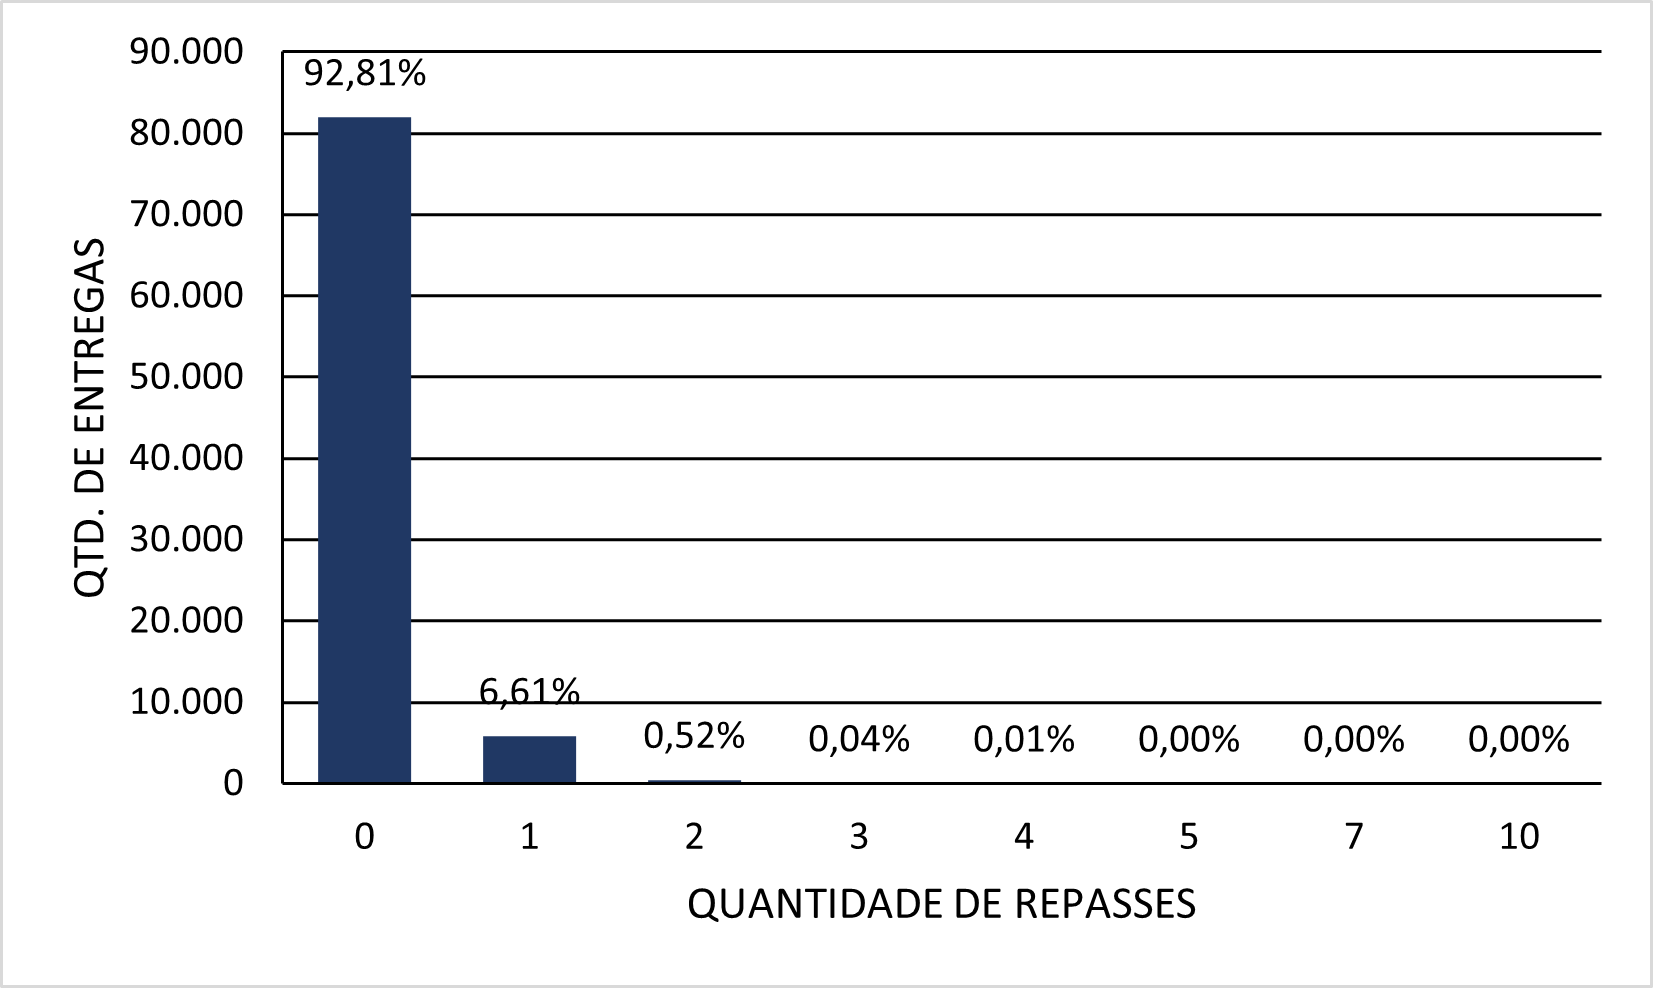
\includegraphics[width=0.5\textwidth]{images/5_emp_bebidas/excel_based/qtde_repasses1.png}
    \caption*{\ Fonte: Produzido pelos autores Fernandes \& Alves}
    \label{fig:Repasses}
\end{figure}

Em adição ao histograma da Figura \ref{fig:Repasses}, é possível observar as ocorrências de repasses nas rotas como um todo a partir da Figura \ref{fig:RepassesRotasBebidas}.
Nela, verifica-se, como supramencionado, que 52\% das rotas apresentam ao menos 1 repasse, sendo que a quantidade máxima de repasses ocorridos em uma única rota no intervalo estudado foi de 20 repasses.
Ademais, identifica-se que 93\% das rotas têm até 4 repasses e 99\% das rotas têm até 9 repasses.

\begin{figure}[H]
    \centering
    \caption{Histograma da quantidade de repasses sofrido por cada cada rota.}
    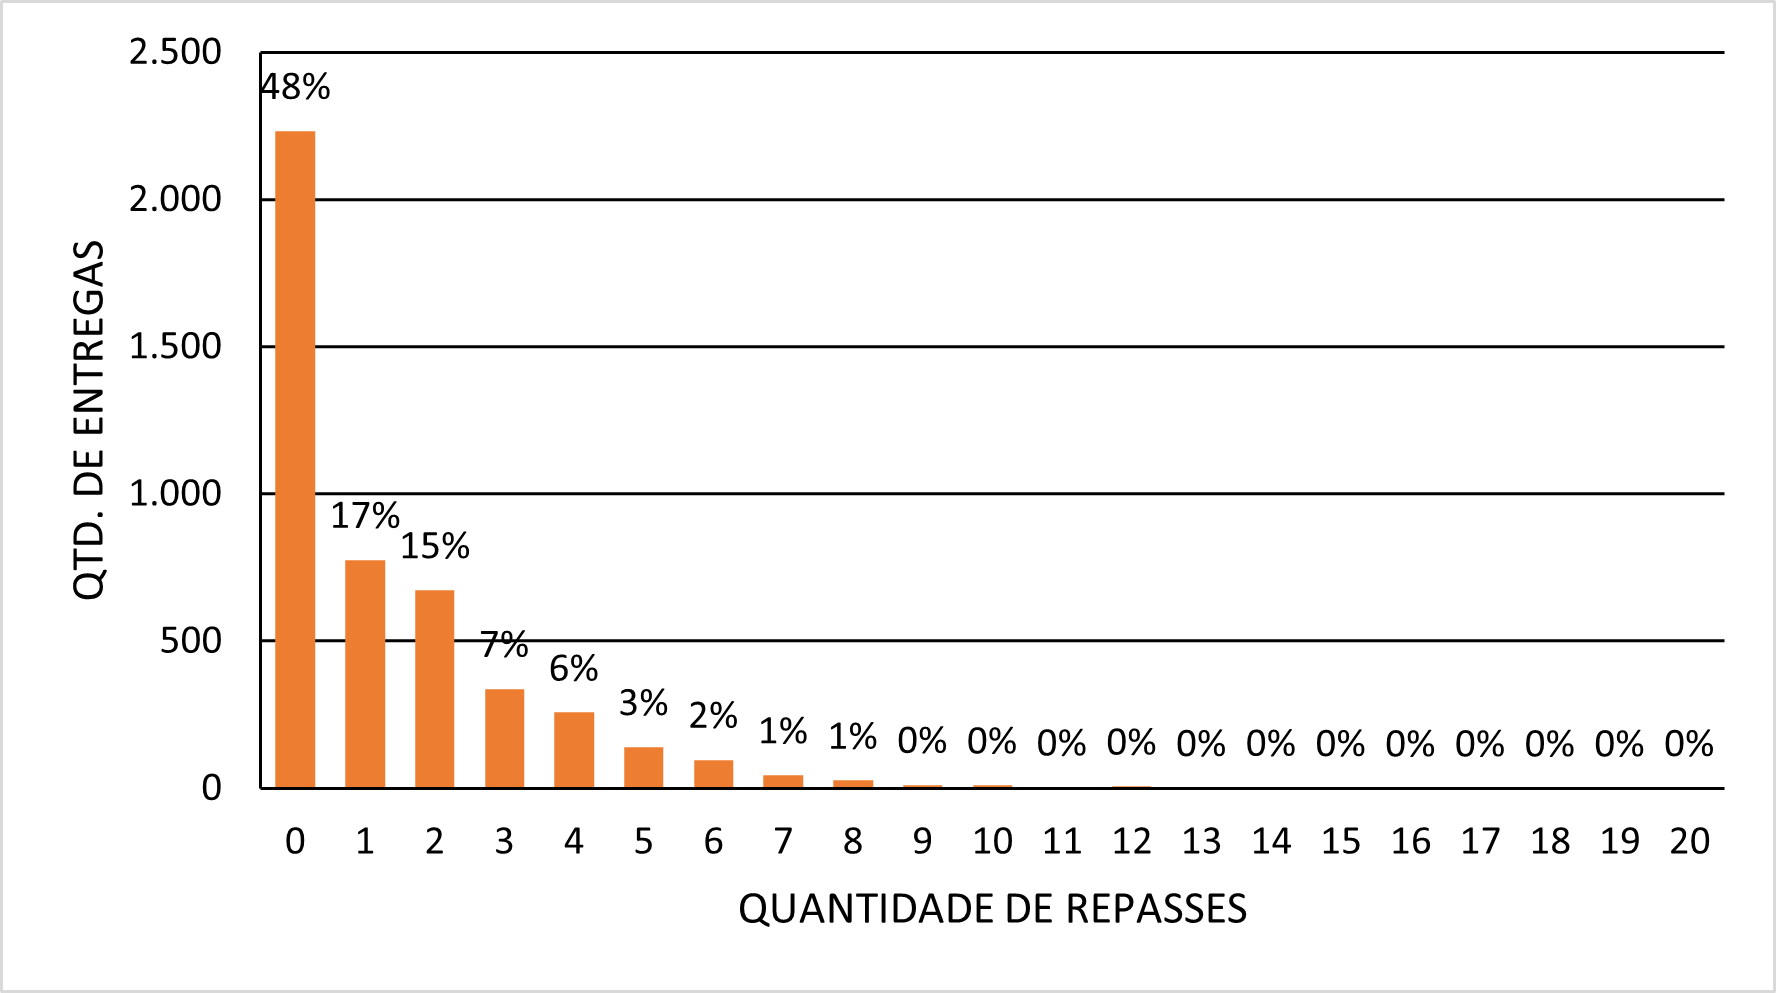
\includegraphics[width=0.5\textwidth]{images/5_emp_bebidas/excel_based/qtde_repasses2.png}
    \caption*{\ Fonte: Produzido pelos autores Fernandes \& Alves}
    \label{fig:RepassesRotasBebidas}
\end{figure}

Em sequência, as devoluções representam 2,1\% do volume total de entregas na amostra de dados explorada na presente pesquisa. 
Tais devoluções ocorreram em 3,2\% das entregas discretizadas.

Finalmente, com intuito de simplificar o entendimento do presente tópico, estabelece-se a Tabela \ref{tab:Variaveis_Problema}, onde é possível observar as principais características citadas de cada medida principal do problema. O restante do trabalho discorrerá, essencialmente, sobre estas três variáveis e quanto à sua relação com outros aspectos intrínsecos à operação ou à configuração da malha viária.

\singlespacing
\begin{table}[htb]
    \centering
    \caption{Resumo das variáveis do problema identificados preliminarmente.}
    \begin{tabular}{|c|c|c|}
    \rowcolor[HTML]{BFBFBF} 
    \hline
    \textbf{Variável} & \textbf{Descrição} & \textbf{Ocorrência} \\ \hline
    Repasse & \begin{tabular}[c]{@{}c@{}}Entregas não realizadas em primeira tentativa.\end{tabular} & 7,2\% \\
    Devolução & \begin{tabular}[c]{@{}c@{}}Volume não entregue e devolvido para o CD.\end{tabular} & 2,1\% \\
    NAS & \begin{tabular}[c]{@{}c@{}}Entrega realizada em sequência diferente da planejada.\end{tabular} & 91,4\% \\ \hline
    \end{tabular}%}
    \caption*{Fonte: Produzido pelos autores Fernandes \& Alves}
    \label{tab:Variaveis_Problema}
\end{table}
\onehalfspacing

Por fim, cita-se que na amostragem do estudo de caso da empresa de bebidas, 91,4\% das entregas feitas tiveram uma alteração em suas ordens sequenciais, valor bastante expressivo e que significa dizer, com efeito, que apenas 8\% das entregas ocorreram de acordo com a ordem ou sequência planejada. Apesar de ser a variável mais frequente apresentada, ela tem um menor impacto direto na perspectiva macroscópica da empresa quando comparada com a devolução, por exemplo, a qual implica no não faturamento de produtos e, portanto, gera maior preocupação para o cotidiano da empresa. 

%%%%%%%%%%%%%%%%%%%%%%%%%%%%%%%%%%%%%%%%%%%%%%%%%%
\section{Impactos econômicos, ambientais e legais} \label{sec:impactoBebidas}

Como detalhado na Seção \ref{RelevanciaTema}, a problemática estudada no presente trabalho acarreta em efeitos negativos de caráter econômico, social e ambiental. Assim, no âmbito do estudo de caso da empresa de bebidas brasileira, é possível definir dois parâmetros primordiais a partir da base de dados fornecida para entender e quantificar tais impactos: distância adicional percorrida e tempo extraordinário de entrega.

A distância adicional percorrida em um roteiro de entregas é caracterizada pela distância que o veículo percorre além do que estava previsto inicialmente para realização de todas as entregas. 
Conforme apresentado por \citeonline{FLAVIOetal}, o processo de roteirização no estudo de caso em questão - que trata da mesma base de dados da empresa de bebidas - apresentou tendência de se superestimar a distância a ser percorrida pelo veículo de entrega, resultando em erros de programação de distância na casa de 30\%, em média.
De fato, a Figura \ref{fig:DistPlan_vs_distReal} ilustra a distribuição de distâncias reais percorridas em comparação com a distância programada, totalizando mais de 15.000 km percorridos adicionalmente.
Esta distância excedente pode resultar em um acréscimo de custos operacionais para a empresa em questão, devido ao maior consumo de combustíveis, maior custo de manutenção associado à utilização dos veículos e também ao maior custo da cadeia de recursos humanos (motorista, auxiliares, entre outros) que afetam a sustentabilidade do sistema operacional.

\begin{figure}[ht]
    \centering
    \caption{Comparativo entre distância real percorrida e distância planejada de cada rota}
    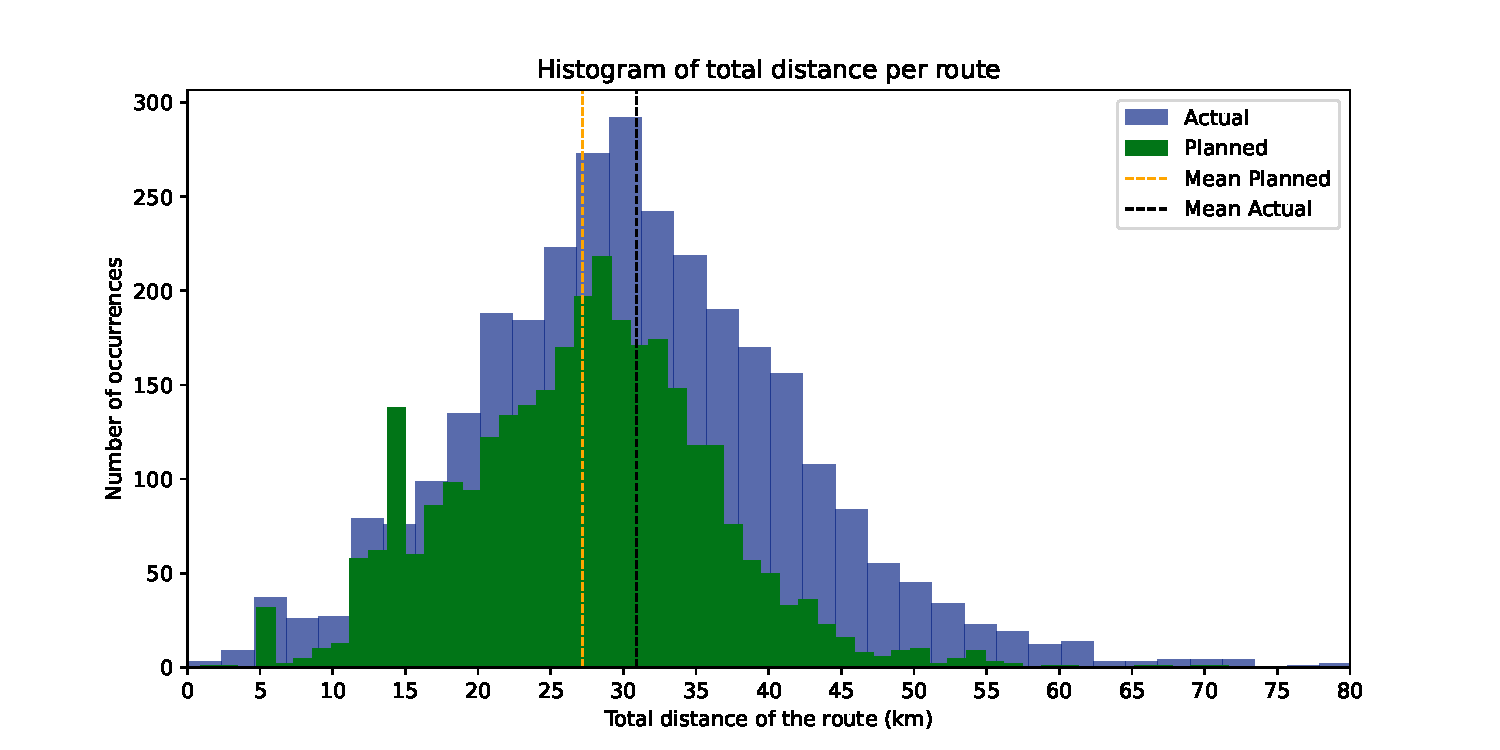
\includegraphics[width=0.8\textwidth]{images/5_emp_bebidas/excel_based/distances_histogram.pdf} 
    \caption*{\ Fonte: Produzido pelos autores Fernandes \& Alves}
    \label{fig:DistPlan_vs_distReal}
\end{figure}

Por outro lado, a distância adicional percorrida impacta, também, ambientalmente devido à emissão de gases contribuintes ao efeito estufa.
Se for considerado que um veículo típico de entregas urbanas consome cerca de 1 litro de diesel a cada 5,5 quilômetros percorridos, considerando-se o consumo urbano de gasolina de um \textit{Volkswagen Delivery Express 2.8} como referência \citeonline{Ramos2021} e que há uma emissão média de 3,2 kg de \ce{CO2} por litro de diesel consumido (que inclui a produção, a distribuição e a queima do diesel, como estimado por \citeonline{Carvalho2011}, a quilometragem percorrida extraordinariamente durante os seis meses de operação analisados passa a representar um total de cerca 7,9 toneladas (t) \ce{CO2} emitidos.
Ou seja, em média são gerados em torno de 16 toneladas adicionais de \ce{CO2} por ano somente no CD estudado.

Finalmente, a Figura \ref{fig:DistPlan_vs_distReal_CORRELACAO} apresenta a correlação entre distância real percorrida e distância planejada levantada pelos autores, obtendo-se a relação de cerca de 10\%, valor abaixo do evidenciado por \citeonline{FLAVIOetal} porém ainda assim representativo para as análises do presente trabalho.

\begin{figure}[ht]
    \centering
    \caption{Distância real percorrida em função da distância planejada}
    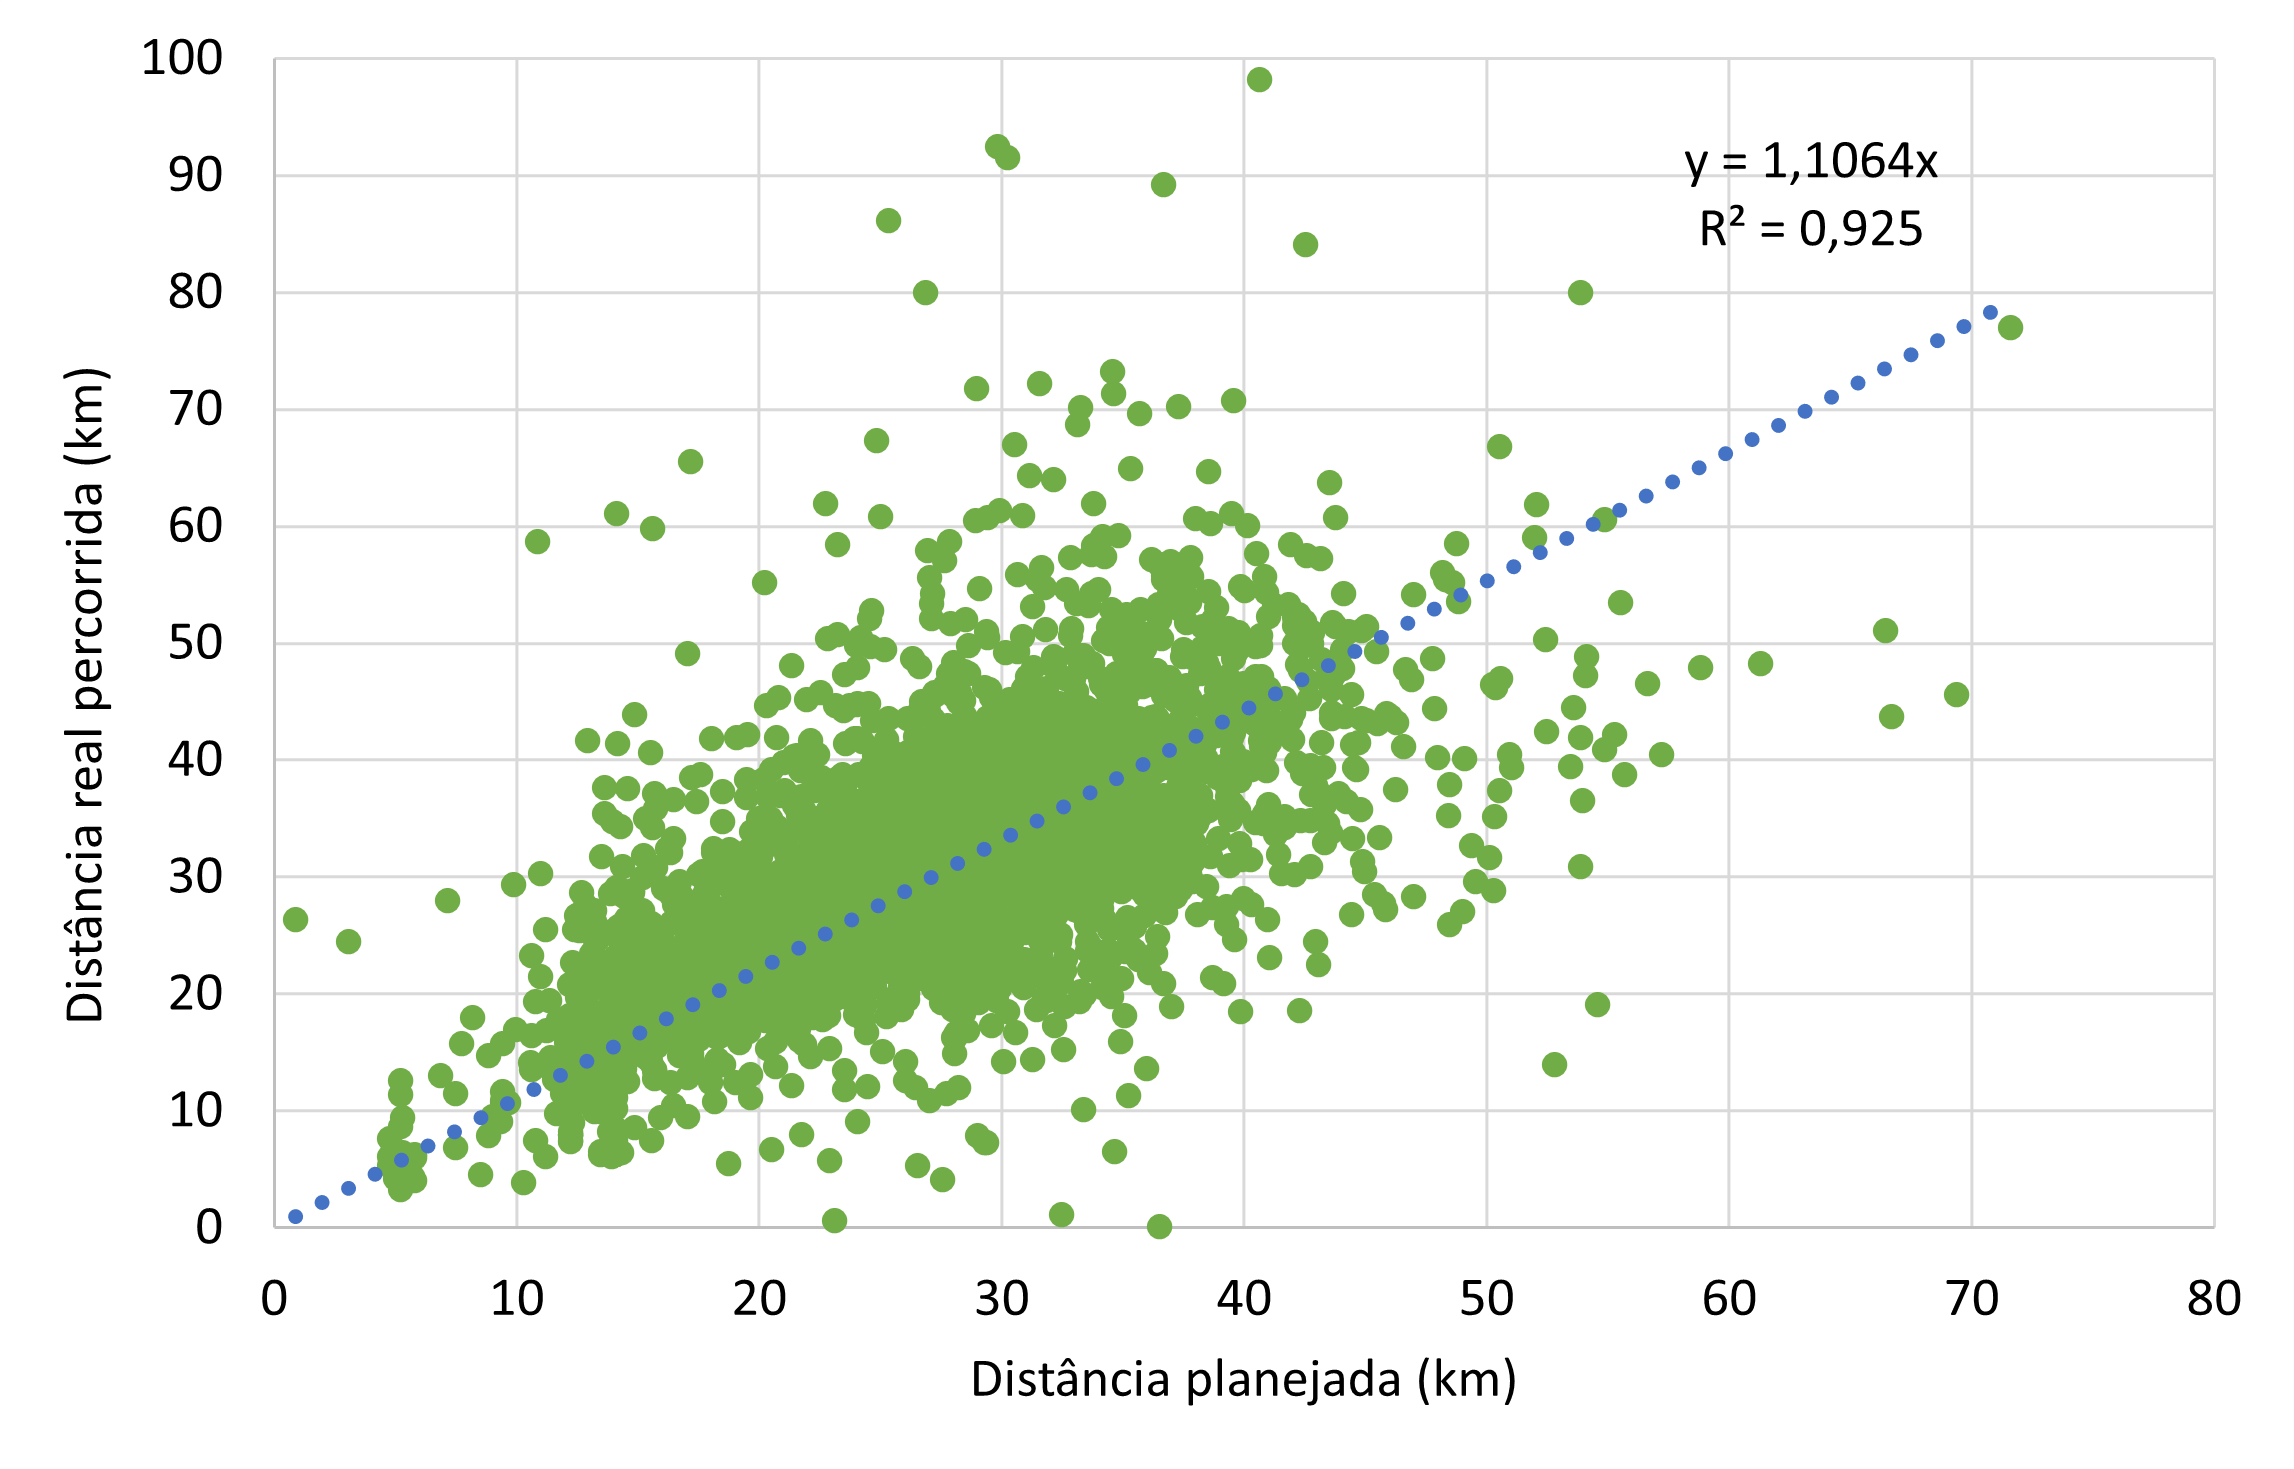
\includegraphics[width=0.6\textwidth]{images/5_emp_bebidas/excel_based/dist_plan_vs_real.png} 
    \caption*{\ Fonte: Produzido pelos autores Fernandes \& Alves}
    \label{fig:DistPlan_vs_distReal_CORRELACAO}
\end{figure}

Outro parâmetro que pode ser analisado a fim de se caracterizar o impacto de não aderência é o tempo extraordinário de entrega, que por sua vez poderá implicar em problemas legais à empresa devido questões trabalhistas. Como apresentado por \citeonline{FLAVIOetal}, para cada conjunto de entregas por veículo há uma forte preocupação em manter a jornada líquida abaixo de 10h20, que é o limite permitido de acordo com a legislação trabalhista. Sendo assim, uma vez que atrasos relacionados à não aderência pode afetar o descumprimento da limitação de jornada de trabalho, há uma preocupação institucional de que o tempo excedente seja controlado e mitigado o máximo possível.

Estes fatores configuram as duas principais fontes de preocupação que justificam o estudo sobre a aderência ao planejamento de entregas no estudo de caso em questão. 

%%%%%%%%%%%%%%%%%%%%%%%%%%%%%%%%%%%%%%%%%%%%%%%%%%%%%%%%%%%%%%%
\section{Visita Técnica}  \label{sec:visita_tecnica}

No dia 17 de junho de 2022 os autores realizaram uma visita técnica ao CD da empresa de bebidas concedente dos dados analisados.
%
É importante destacar que o CD visitado não é o mesmo centro estudado por meio da base de dados, porém para o escopo da pesquisa a diferença entre os dois CDs (visitado e estudado) é considerada desprezível.
%
Ademais, convém ressaltar que há uma lacuna temporal entre os valores observados na base de dados e a realidade observada na prática, visto que a visita ocorreu cerca de sete anos após a coleta de informações para a base de dados estudada.
%
Em sete anos de operação alguns contextos podem se alterar, como é o caso da capacidade, oferta e demanda da empresa, representada pelas variação das quantidades de clientes, SKUs e frota disponível ao longo dos anos.
%
Portanto foi dado foco nos procedimentos que não tenham sido alterados significativamente entre o período de registro dos dados e o momento da visita.
%

De início, uma primeira informação que se destacou para os autores durante a visita foi a diferenciação dos veículos de entrega de acordo com a sua capacidade.
Embora acreditava-se que os veículos eram todos de um mesmo modelo, o que se verificou por meio da visita foi que a empresa opera com pelo menos 3 tipos diferentes de caminhões por dia, sendo eles: caminhão 6 baias, caminhão 10 baias e caminhão \textit{bi-truck}.
Os caminhões modelo \textit{bi-truck} são de maior capacidade, e portanto atendem somente clientes que exigem volumes de entrega mais elevados, como é o caso de supermercados e outros clientes de segmento \textit{off-trade}, i.e. que em geral funcionam como ponto de revenda para o consumidor e não como estabelecimento de consumo. 
As entregas do \textit{on-trade} por sua vez são realizadas pelos caminhões de 6 ou de 10 baias, a depender do volume de entregas. 
É importante destacar que durante o trabalho foram estudadas apenas entregas relativas ao segmento de \textit{off-trade}, visto que é neste setor que o número de entregas por veículo é de fato expressivo.
A decisão sobre qual tipo de veículo utilizar para cada rota é tomada pelo software de roteirização da empresa, que será descrito mais abaixo.

Outro aspecto importante descoberto durante a visita foi a relação entre os tipos de veículo e a largura das vias.
Por se tratar especialmente de uma região metropolitana e até mesmo periférica da cidade de São Paulo, alguns dos clientes estão posicionados em ruas paralelas de menor largura, o que em alguns casos impede a utilização de veículos de capacidade mais elevada, que é o caso dos caminhões de 10 baias.
Desta forma, durante a etapa de planejamento o time de especialistas necessita verificar a compatibilidade entre PDEs e capacidade do caminhão, podendo realizar alguns ajustes que estejam mais visíveis.
Contudo nem sempre é possível determinar as rotas ideais uma vez que informações de largura de via não são de fácil acesso aos usuários comuns, tampouco para os especialistas de planejamento.
O que se faz para contornar essa situação, em geral, é padronizar a equipe de entregas por região e veículo, de modo que um mesmo motorista tenda a percorrer percursos similares e dessa forma já consiga prever de antemão quais os empecilhos que podem se apresentar durante a rota.

Adicionalmente identificou-se uma possível segmentação de clientes durante a visita. 
Foi mencionado que alguns clientes recebiam prioridade de entrega por participarem de algum programa de clientes \textit{``VIPs''}, o que poderia significar em piores valores de NAS devido a uma estratégia customizada da empresa. 
Tal aspecto evidencia uma limitação da base de dados descrita na seção \ref{sec:realidade_empresa}, uma vez que não houve qualquer diferenciação entre os tipos de clientes.

Já quanto à programação das rotas em si, esta é realizada diariamente através de \textit{software} solução de mercado obtido pela empresa e utilizada em escala nacional pelos seus diferentes CDs.
Diariamente a equipe de planejamento precisa atualizar no sistema da empresa qual é a disponibilidade real de frota para realização de entregas do dia seguinte, este cadastro ocorre por volta das 17 horas, ou seja, quase no final do expediente.
Uma vez cadastrados os dados no sistema, a roteirização será feita em segundo plano utilizando como base os pedidos que foram confirmados pelos clientes até o fim do dia.
O processo não leva mais de duas horas para ser concluído, porém ao se obter o resultado da roteirização muitas vezes são realizados diversos ajustes manuais de modo a compatibilizar o resultado extraído do simulador com a realidade experienciada pelos planejadores e operação.

Durante o expediente de operação, que geralmente vai de 8 da manhã até 7 da noite em dias convencionais, a equipe de planejamento de rotas fica disposta no CD da empresa em local dedicado exclusivamente para acompanhamento das entregas e replanejamento de tentativas mal-sucedidas. 
Sempre que uma entrega não pôde ser realizada, a equipe de planejamento é acionada para verificar qual o melhor horário para a operação retornar ao PDE naquele dia, além de registrar os motivos da não realização das entregas.
Um painel em formato de \textit{dashboard} é utilizado para acompanhamento das rotas de entrega ao longo do expediente, conforme evidenciado na Figura \ref{fig:painel_repasses}, em que cada linha representa uma rota diferente e cada círculo representa um diferente PDE.
A cor verde indica que a entrega naquele PDE foi concluída com sucesso, a vermelha significa que não foi possível entregar e que está confirmado que haverá devolução, enquanto que a cor roxa indica que já foi feita tentativa sem sucesso porém a entrega foi remarcada para outro horário (ou seja, ocorrência de repasse).

\begin{figure}[htb]
    \centering
    \caption{Painel de acompanhamento das rotas de entregas registrado no dia da visita}
    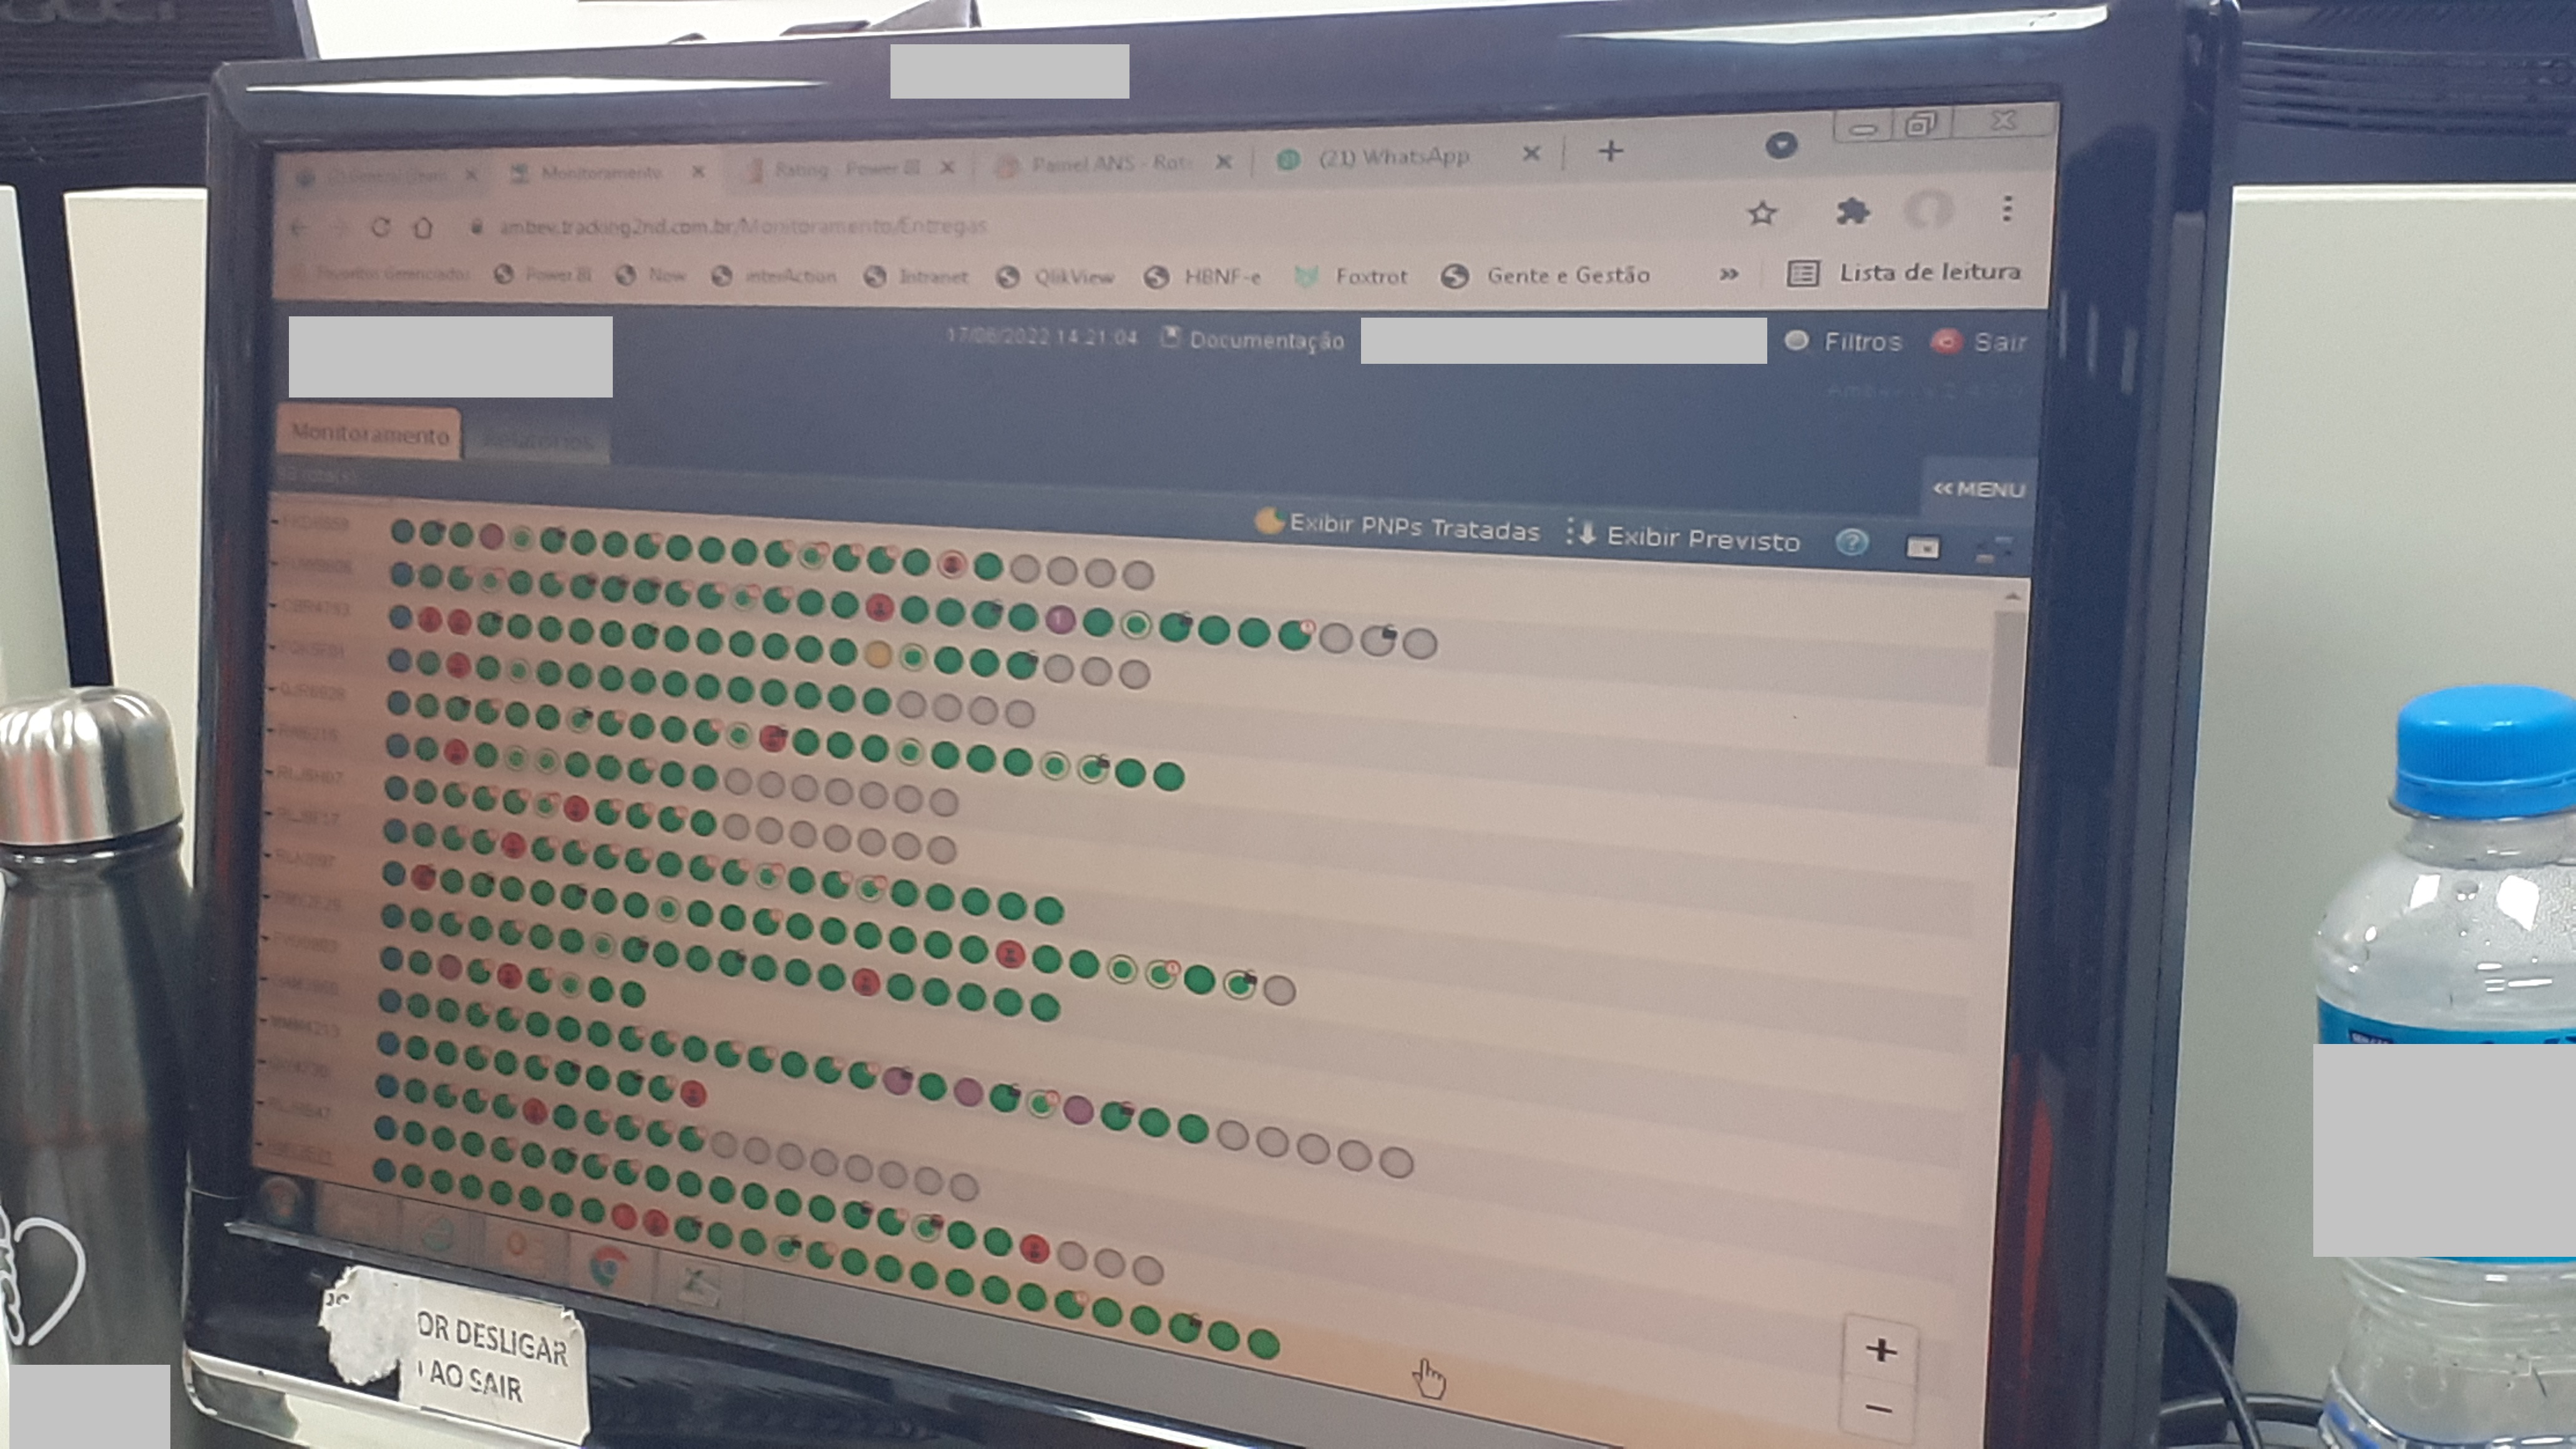
\includegraphics[width=0.8\textwidth]{images/5_emp_bebidas/painel_rotas_CDD_diadema.jpg}
    \caption*{Fonte: Produzido pelos autores Fernandes \& Alves}
    \label{fig:painel_repasses}
\end{figure}

Ademais, através contato direto com a equipe operacional, foi possível estabelecer novas linhas de análise, antes não consideradas. Uma tese levantada conjuntamente, foi de que o calendário (dia da semana, época do mês, feriados, etc.) pode ter influência direta nos problemas estudados. 
%
Outra informação relevante que pôde ser estabelecida na visitação técnica foi acerca do quão rigorosa a equipe operacional é com devoluções. Eles estabelecem um critério de bloqueio dos PDE que apresentam reincidência de devoluções, ou seja, que realizam devoluções repetidamente. Essa informação, futuramente, pode ser considerada na possibilidade de se observar, na base de dados, qual o comportamento, ao longo do tempo, para com os PDEs com maiores índices de devoluções.

A visita técnica em questão possibilitou a adição de conceitos e visões externas ao trabalho, de modo que os autores puderam validar algumas das hipóteses e, principalmente, entender na prática como funcionam algumas das rotinas de distribuição de entregas de última milha na região estudada.


%%%%%%%%%%%%%%%%%%%%%%%%%%%%%%%%%%%%%%%%%%%%%%%%%%%%%%%%%%%%%%%
\section{Perfil das rotas} \label{sec:analise_base_dados}

Ao inspecionar a base de dados disponibilizado para o estudo, elencou-se cinco parâmetros que poderiam apresentar alguma correlação com os problemas estudados, são eles: Posição sequencial do PDE dentro de sua rota; Frequência média de entregas do PDE; Veículo utilizado para realizar a entrega; Horário em que a entrega foi realizada; e Volume de caixas da entrega.
Estes valores bem como a relação com o problema atual estão descritos nos itens a seguir.

\subsection{Posição Sequencial}

Como apresentado na seção \ref{sec:realidade_empresa}, a base de dados inclui informação sobre qual posição cada PDE ocupou na sequência de entregas de cada rota.
É possível induzir que a posição que o PDE ocupou na sequência de entregas pode ser relevante para explicar alguns dos fenômenos analisados.
Isso se dá pela tese de que os motoristas podem ter problemas mais frequentemente com alguma posição específica da sequência, especialmente as mais extremas – primeiras ou últimas.

Desta forma, identificou-se que, a NAS tem uma relação proporcional com a variável ``posição sequencial'', enquanto os repasses apresentam uma relação inversamente proporcional, como observa-se nas Figuras \ref{fig:PosicaoSequencial} e \ref{fig:PosicaoSequencialRS}.

\begin{figure}[H]
    \caption{Correlação entre fenômeno estudado e a posição sequencial do PDE na rota.}
    \begin{subfigure}{.64\textwidth}
        \centering
        % include first image 
        \caption{Relação Gráfica entre as variáveis e a Posição Sequencial.}
        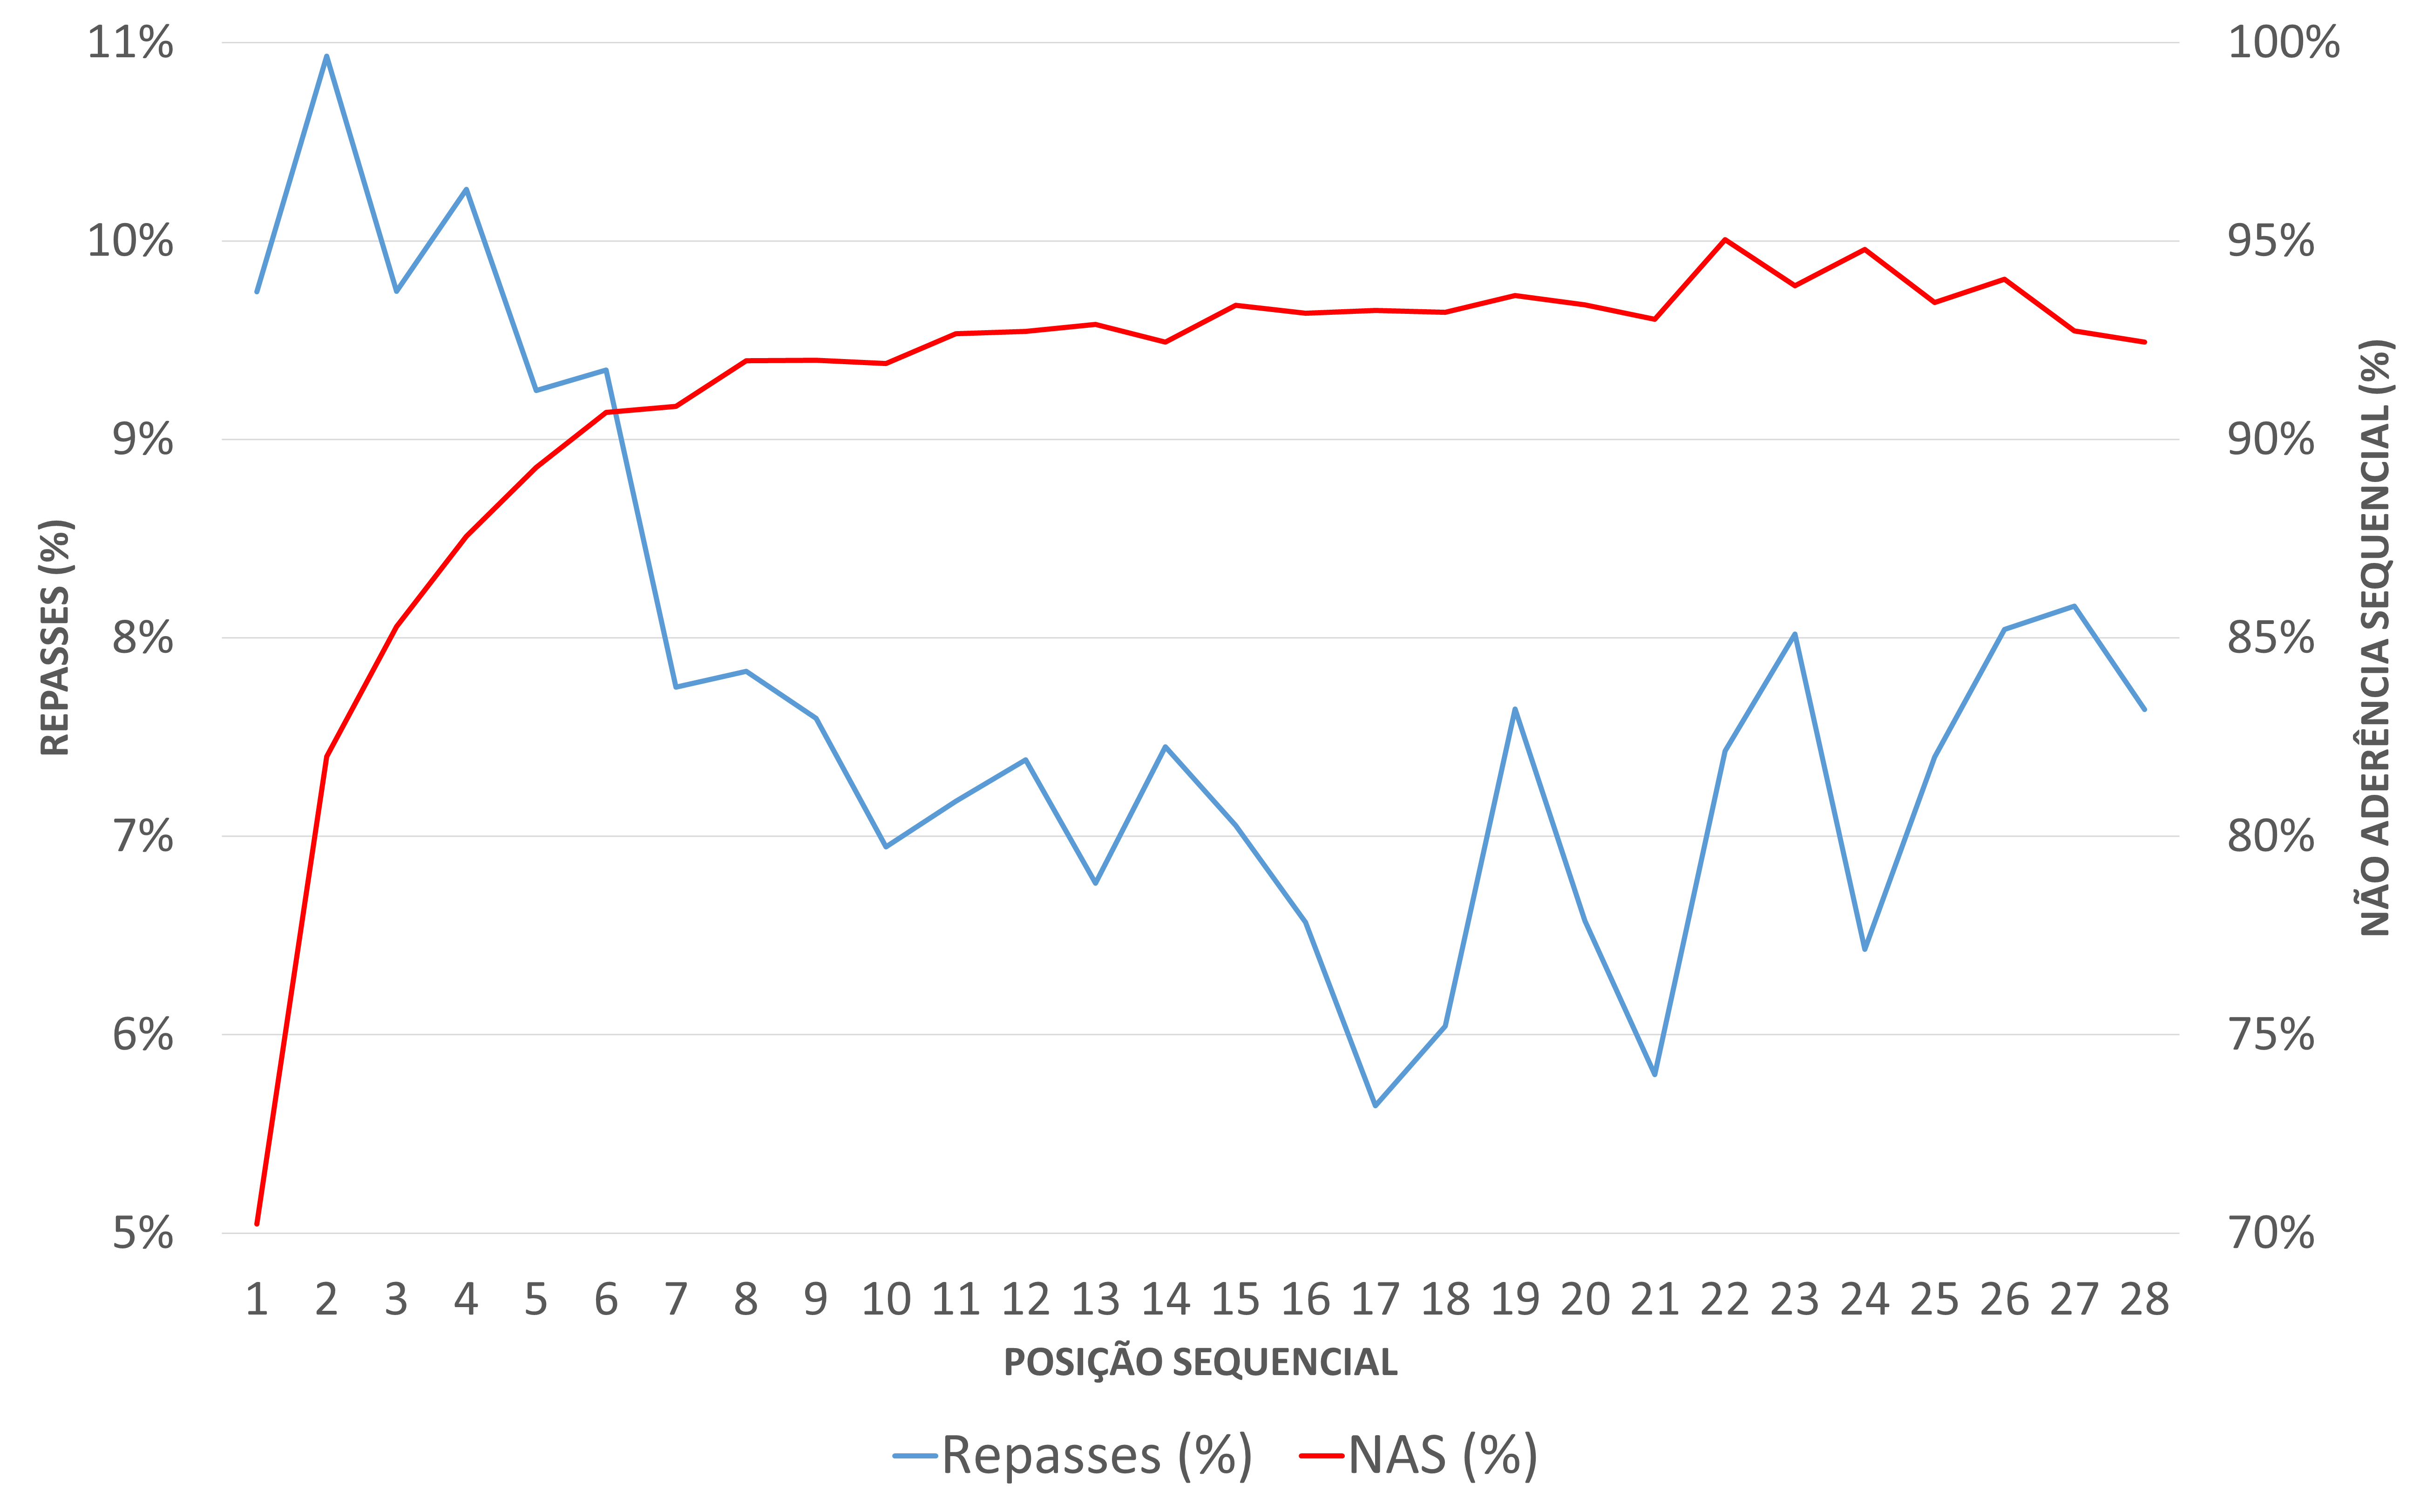
\includegraphics[width=.98\linewidth]{images/5_emp_bebidas/excel_based/PosicaoSequencial.png}
        \label{fig:PosicaoSequencial}
    \end{subfigure}
    \begin{subfigure}{.35\textwidth}
      \centering
      % include second image
      \caption{Estatísticas da Regressão Linear.}
      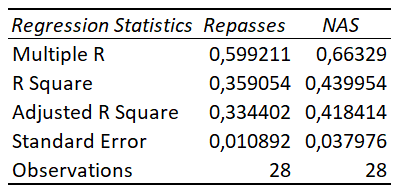
\includegraphics[width=.88\linewidth]{images/5_emp_bebidas/excel_based/PosicaoSequencial_RS.png}
      \label{fig:PosicaoSequencialRS}
    \end{subfigure}
    \caption*{\ Fonte: Produzido pelos autores Fernandes \& Alves}
\end{figure} % Posicao Sequencial

É importante destacar que a relação observada, porém, é inversa para cada problema. 
Ou seja, identifica-se que a ocorrência de repasses é maior nas primeiras posições, enquanto a aderência sequencial é menor nas últimas posições.
Assim, observa-se que cada problema, mesmo tendo um comportamento único, pode ser explicado através da mesma variável.

\subsection{Frequência}

A partir da base de dados fornecida, outra informação que é possível construir é a frequência média de entregas que cada PDE recebe. 
Isso pode ser obtido a partir da informação da data em que foi realizada cada entrega. 
Tal informação, empiricamente, pode ser estabelecida como uma potencial variável relacionada aos problemas estudados, assumindo-se que o motorista do veículo de entregas pode ser influenciado positivamente pelo nível de conhecimento que ele tem do PDE – seus receptores, o espaço de descarga, as vias de acesso, etc. 
Por outro lado, estabelece-se a possibilidade de que a alta frequência de entregas em determinado PDE impacte negativamente na aderência ao sequenciamento e/ou nos repasses devido a um vínculo de confiança que pode se estabelecer entre os dois agentes citados e, assim, gerar no motorista confiança suficiente para estabelecer sua própria rotina de entregas, ignorando parcial ou totalmente o sequenciamento gerado pelo roteirizador.

Assim, nas Figuras \ref{fig:Frequencia1} e \ref{fig:Frequencia2} é possível observar a relação entre o percentual de repasses e NAS com a frequência de entregas, obtendo aderência suficiente num primeiro momento.

 \begin{figure}[H]
     \caption{Correlação entre a frequência de entregas no PDE e as variáveis-problema.}
     \begin{subfigure}{.64\textwidth}
         \centering
         % include first image 
         \caption{Relação Gráfica entre as variáveis e a Frequência.}
         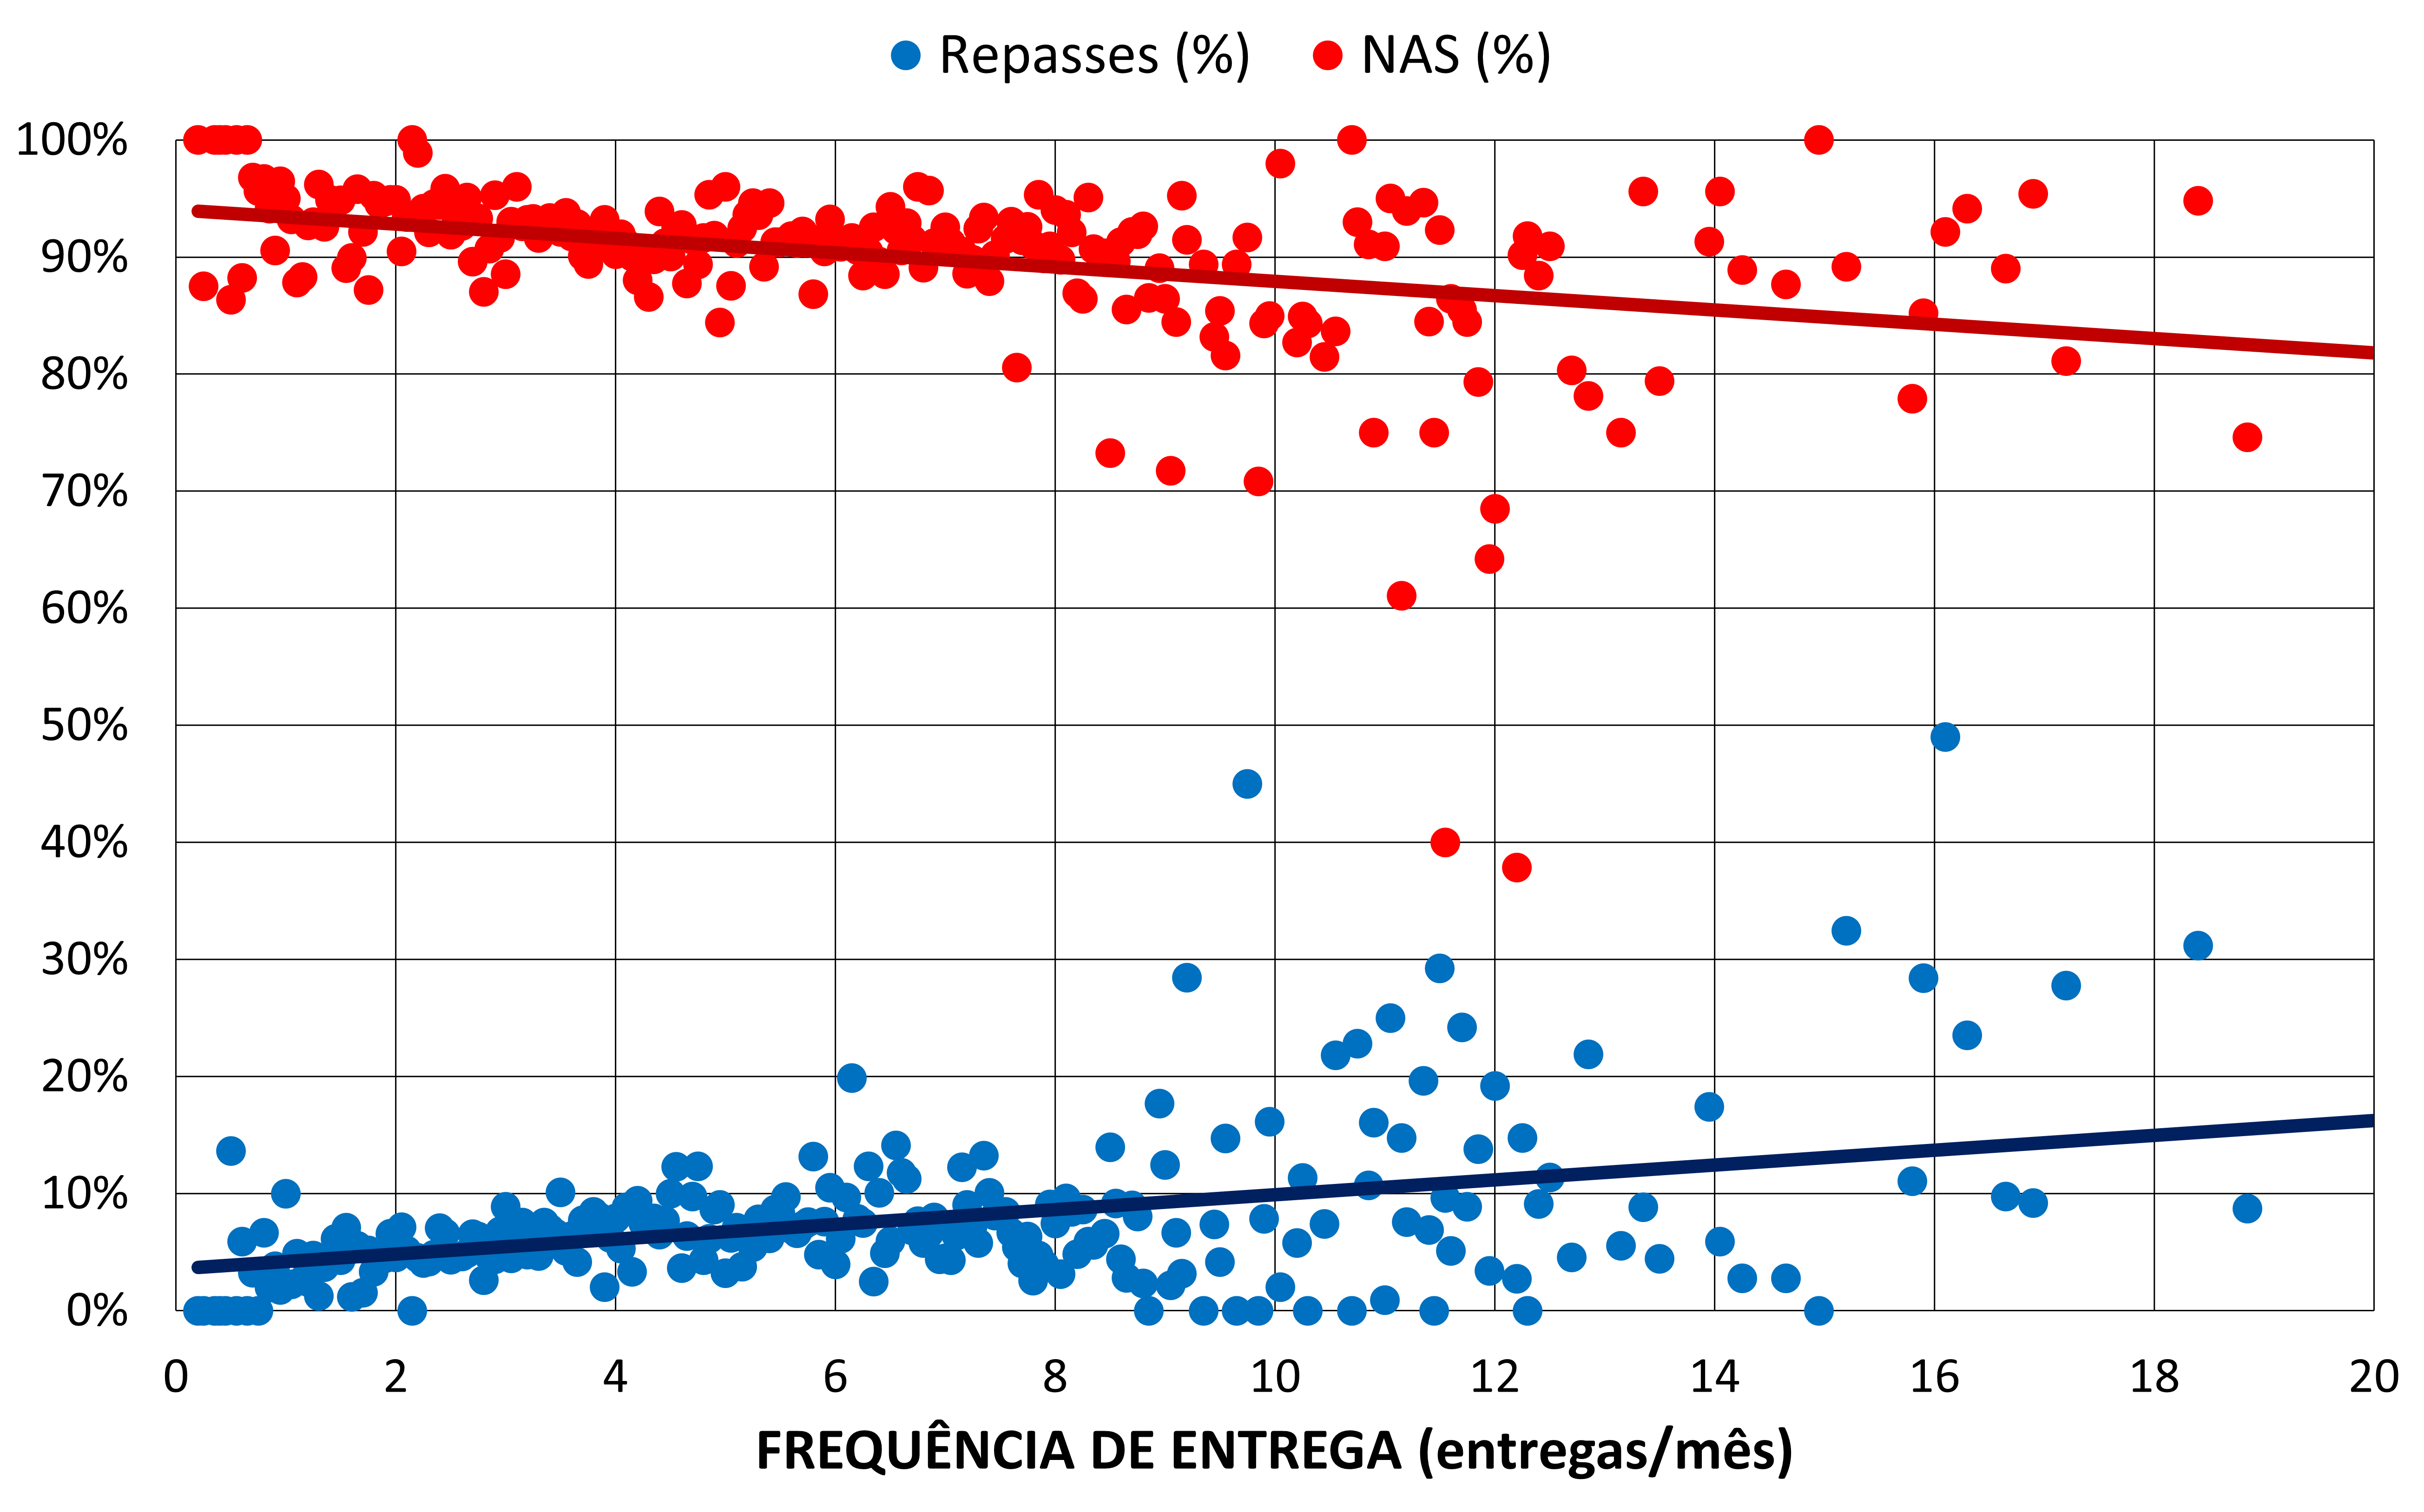
\includegraphics[width=.98\linewidth]{images/5_emp_bebidas/excel_based/Frequencia.png}
         \label{fig:Frequencia1}
     \end{subfigure}
     \begin{subfigure}{.35\textwidth}
       \centering
       % include second image
       \caption{Estatísticas da Regressão.}
       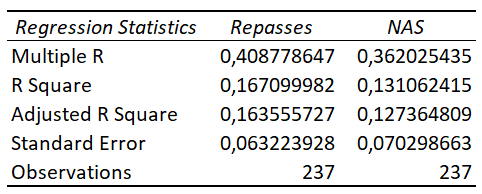
\includegraphics[width=.88\linewidth]{images/5_emp_bebidas/excel_based/Frequencia_RS.png}
       \label{fig:Frequencia2}
     \end{subfigure}
     \caption*{\ Fonte: Produzido pelos autores Fernandes \& Alves}
 \end{figure} % Frequencia

Novamente, observa-se um comportamento inverso no parâmetro como causados dos problemas: enquanto frequências altas (0 $<$ T $<$ 10 dias) indicam maior incidência de repasses, são as frequências baixas (12 dias $<$ T) que apresentam baixa aderência.

Um comentário relevante a se fazer em relação a esta análise é de que a frequência de entregas é uma característica associada ao PDE, reduzindo, assim, a amostragem utilizada para a correlação.
Isso se dá pois, em outras análises, tais como a de posição sequencial, a variável é associada a cada entrega realizada (total de 88.338 entregas), enquanto a frequência é associada ao PDE (total de 4.554 PDEs).

\subsection{Veículo}

Outra análise que pode ser realizada a partir dos dados disponibilizados na base de dados é a contribuição do veículo utilizado para as entregas. 
Na base, é possível identificar qual a placa relativa ao veículo utilizado em cada rota. 
Tal análise pode ser validada a partir da informação obtida através da visitação técnica, como visto na seção \ref{sec:visita_tecnica}, de que o planejamento de entregas busca unificar os veículo à equipe (motorista e ajudante(s)) o mais frequentemente o possível. 
Assim, uma correlação pode insurgir da tese de que cada equipe possui preferências e peculiaridades específicas ao seu comportamento e experiência.

Desta forma, foi investigada a correlação entre a placa veicular e os indicadores de repasse e NAS, como pode ser observado na Figura \ref{fig:Veiculo}, onde é possível identificar a ocorrência de uma possível correlação com ambos os indicadores, demonstrando que algumas equipes podem ter maior tolerância aos repasses e à NAS do que outras.

\begin{figure}[H]
    \centering
    \caption{Comparação entre NAS e repasse para os diferentes veículos utilizados.}
    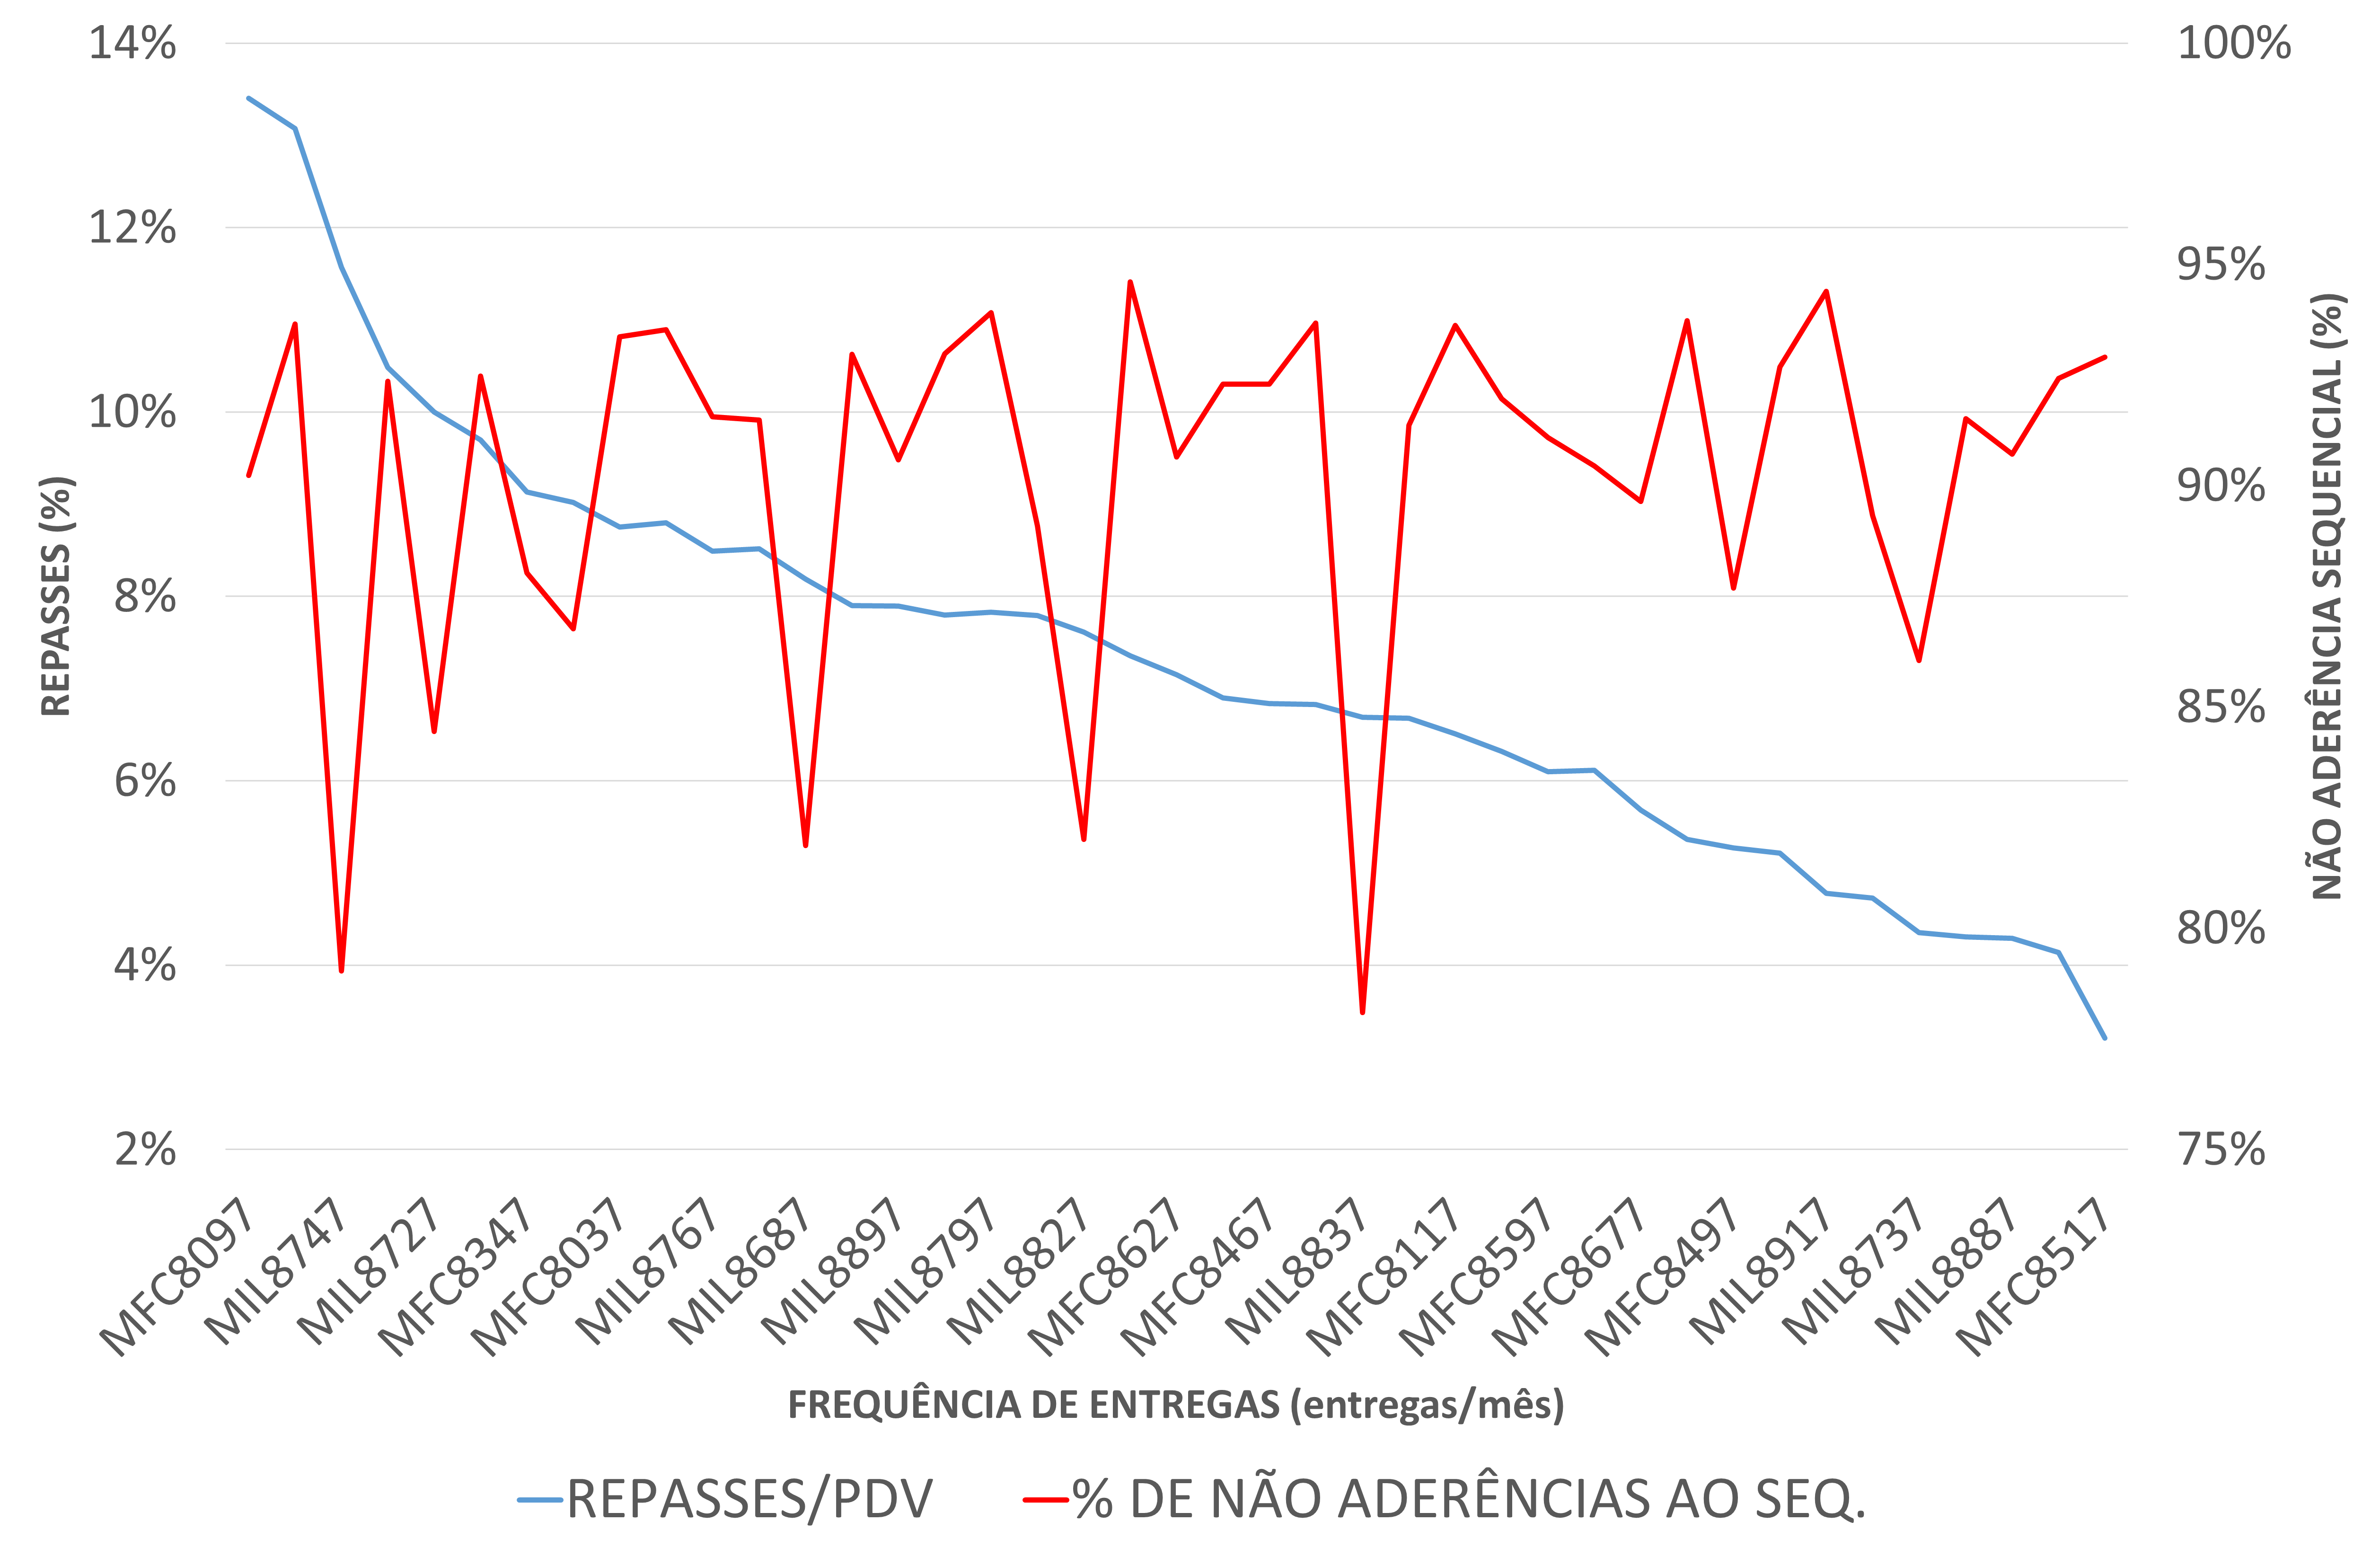
\includegraphics[width=0.8\textwidth]{images/5_emp_bebidas/excel_based/Veiculo.png}
    \caption*{\ Fonte: Produzido pelos autores Fernandes \& Alves}
    \label{fig:Veiculo}
\end{figure} % Veiculo

Um fator relevante a se comentar é a escolha da sequência das placas veicular na Figura \ref{fig:Veiculo}. A escolha foi a favor da ordenação decrescente dos valores de repasse para fins visuais. Naturalmente, o gráfico busca salientar que é possível identificar uma variação considerável das variáveis estudadas, quando organizadas por veículo. Deste modo, confirma-se a tese de que determinadas equipes de entrega podem apresentar maiores tendências de realizar repasses ou NAS do que outras.

\subsection{Horário de Entrega}

Outra análise que pode ser realizada é a de correlação entre as variáveis do problema e o horário no qual a entrega foi realizada.
O horário pode revelar uma correlação com a ocorrência de repasses ou NAS considerando-se o comportamento da equipe de entregas e do cliente receptor. 
Ao longo do dia, diferentes fatores podem ser influenciadores de tais ocorrências, tais como, cansaço dos agentes envolvidos, disponibilidade do receptor, trânsito, entre outros.

As Figuras \ref{fig:Horario} e \ref{fig:HorarioRS} mostram a evolução dos valores médios de repasse (\%) e de NAS (\%) ao longo do dia, considerando a série histórica de cinco meses de entregas.

 \begin{figure}[H]
     \caption{Comparação entre Horário de Entrega e variáveis-problema}
     \begin{subfigure}{.64\textwidth}
         \centering
         % include first image 
         \caption{Relação Gráfica entre as variáveis e o Horário.}
         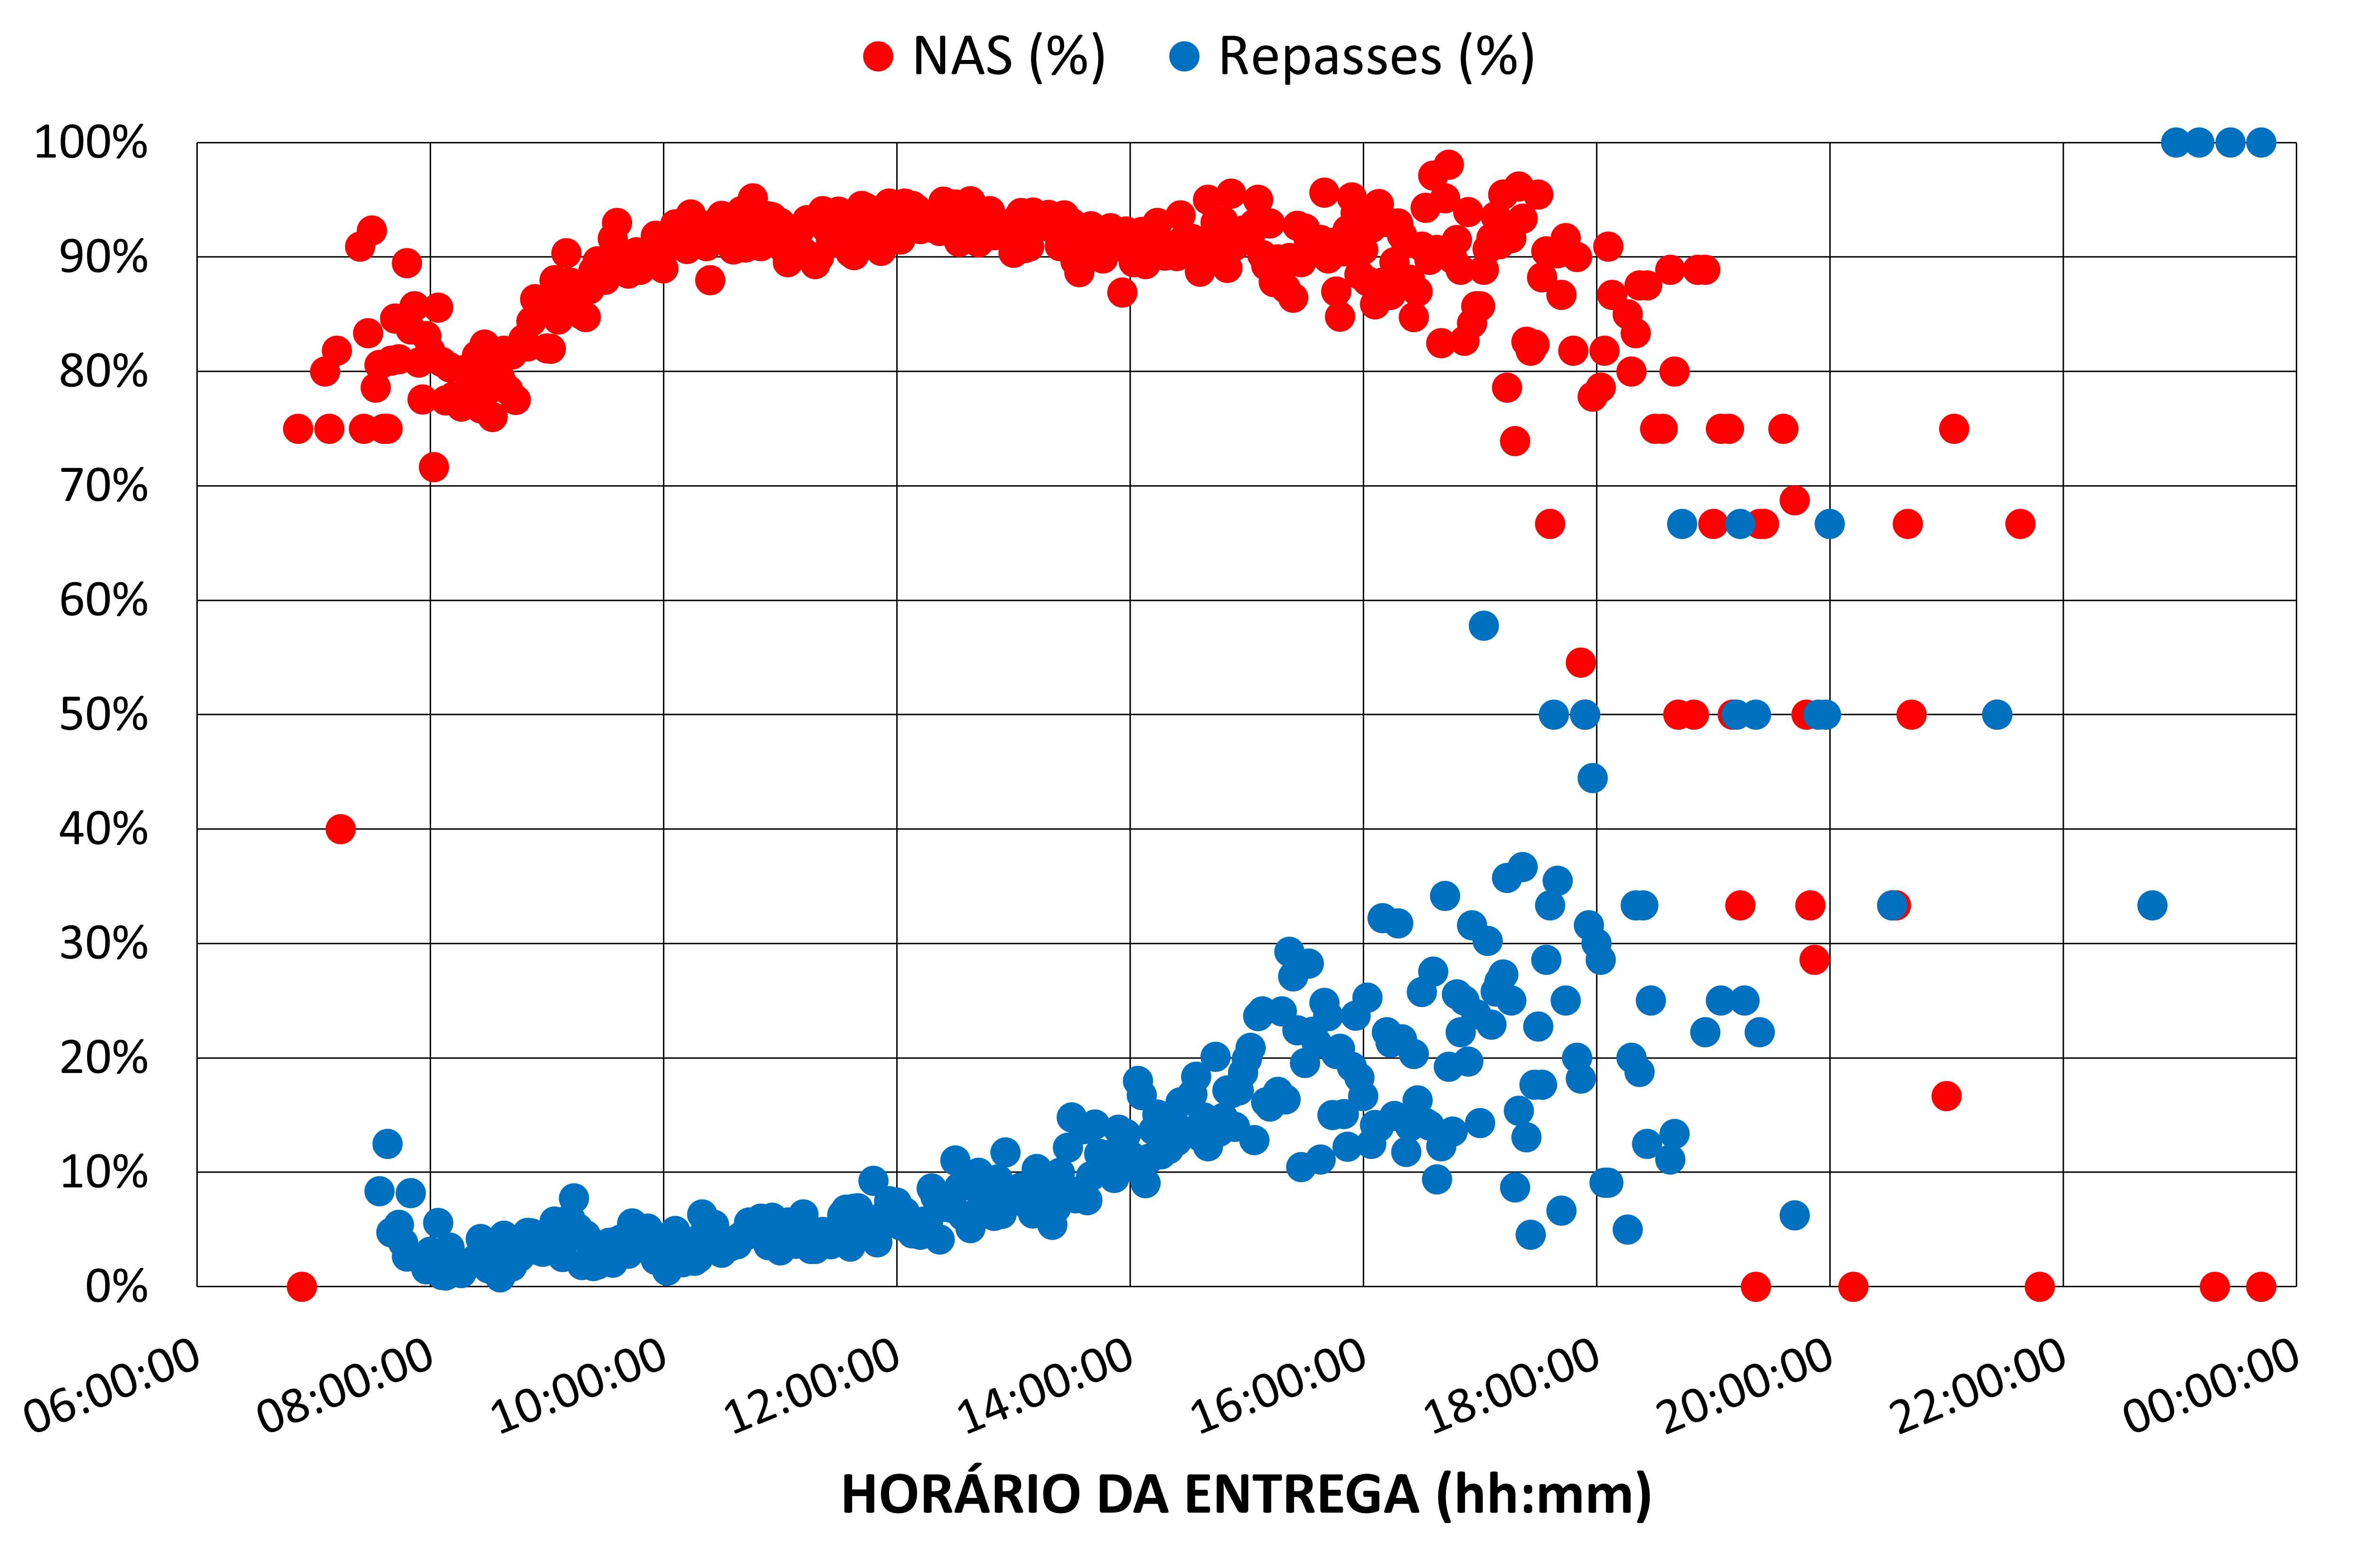
\includegraphics[width=.98\linewidth]{images/5_emp_bebidas/excel_based/Horario.png}
         \label{fig:Horario}
     \end{subfigure}
     \begin{subfigure}{.35\textwidth}
       \centering
       % include second image
       \caption{Estatísticas da Regressão.}
       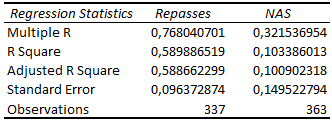
\includegraphics[width=.88\linewidth]{images/5_emp_bebidas/excel_based/Horario_RS.png}
       \label{fig:HorarioRS}
     \end{subfigure}
     \caption*{\ Fonte: Produzido pelos autores Fernandes \& Alves}
 \end{figure} % Horario

Inicialmente, é possível determinar que os primeiros horários do dia são particularmente positivos, apresentando baixos índices de repasses e de NAS. 
Outra informação interessante que pode ser obtida é a de que os horários mais próximos ao almoço (i.e. 11:00 - 13:00) têm maior ocorrência de NAS.
Isso pode ser um indicativo da tendência de alguns clientes ficarem indisponíveis em horários de maior fluxo no setor de restaurantes.
Ademais, isso pode, também, ser um indicativo da tendência da equipe de entregas reajustar seu sequenciamento nas proximidades de sua pausa para almoçar. 
Tal tese, entretanto, pode ser contraposta com a informação adquirida durante visitação presencial de que as equipes em geral tendem a pular o horário de almoço para atingir suas metas e encerrar o horário de trabalho mais cedo.

Por fim, observa-se uma tendência de aumento do volume de repasses ao fim do turno de trabalho. Tal comportamento pode ser explicado pelo costume operacional, identificado na visitação, de se posicionar as revisitas de repasse ao fim do dia.

\subsection{Volume da Entrega}

Também é possível identificar uma variável quantificadora do tamanho de cada entrega que mensura a quantidade de caixas entregues.
Através da visita técnica, verificou-se que a caixa é uma medida padrão estabelecida a partir da garrafeira de entregas média de capacidade de 24 garrafas de 600 ml. 
Outras composições de entregas, tais como os conjuntos de garrafas plásticas de 2 litros ou as latas de alumínio de 350 ml, são convertidas para a unidade de caixas através da equivalência volumétrica.

Intuitivamente, a quantidade de caixas entregues pode apresentar correlação para com as variáveis de repasses e NAS, considerando-se o grau de relevância que a entrega passa a ter para a equipe e o cliente. Assim, volumes maiores a serem entregues podem ser tratados de forma diferente aos volumes menores, o que pode resultar em resultados diferentes entre as variáveis-problema.

Assim, por se tratar de uma variável contínua, foi estabelecida uma análise de correlação através de uma \textit{nuvem de pontos} para cada variável-problema e, em sequência, o destacamento da regressão linear de cada uma.
Nas Figuras \ref{fig:Volume} e \ref{fig:VolumeRS} é possível visualizar essa análise, onde é possível identificar um comportamento de potencial correlação entre o volume entregue e as variáveis.

Cita-se que os cada ponto do gráfico é um PDE. Assim a avaliação é baseada no volume médio recebido por cada PDE no intervalo estudado, assim como seus indicadores de \%REP e \%NAS.

\begin{figure}[H]
     \caption{Correlação entre as variáveis problema e o volume entregue.}
     \begin{subfigure}{.64\textwidth}
         \centering
         % include first image 
         \caption{Relação Gráfica entre as variáveis e o Volume.}
         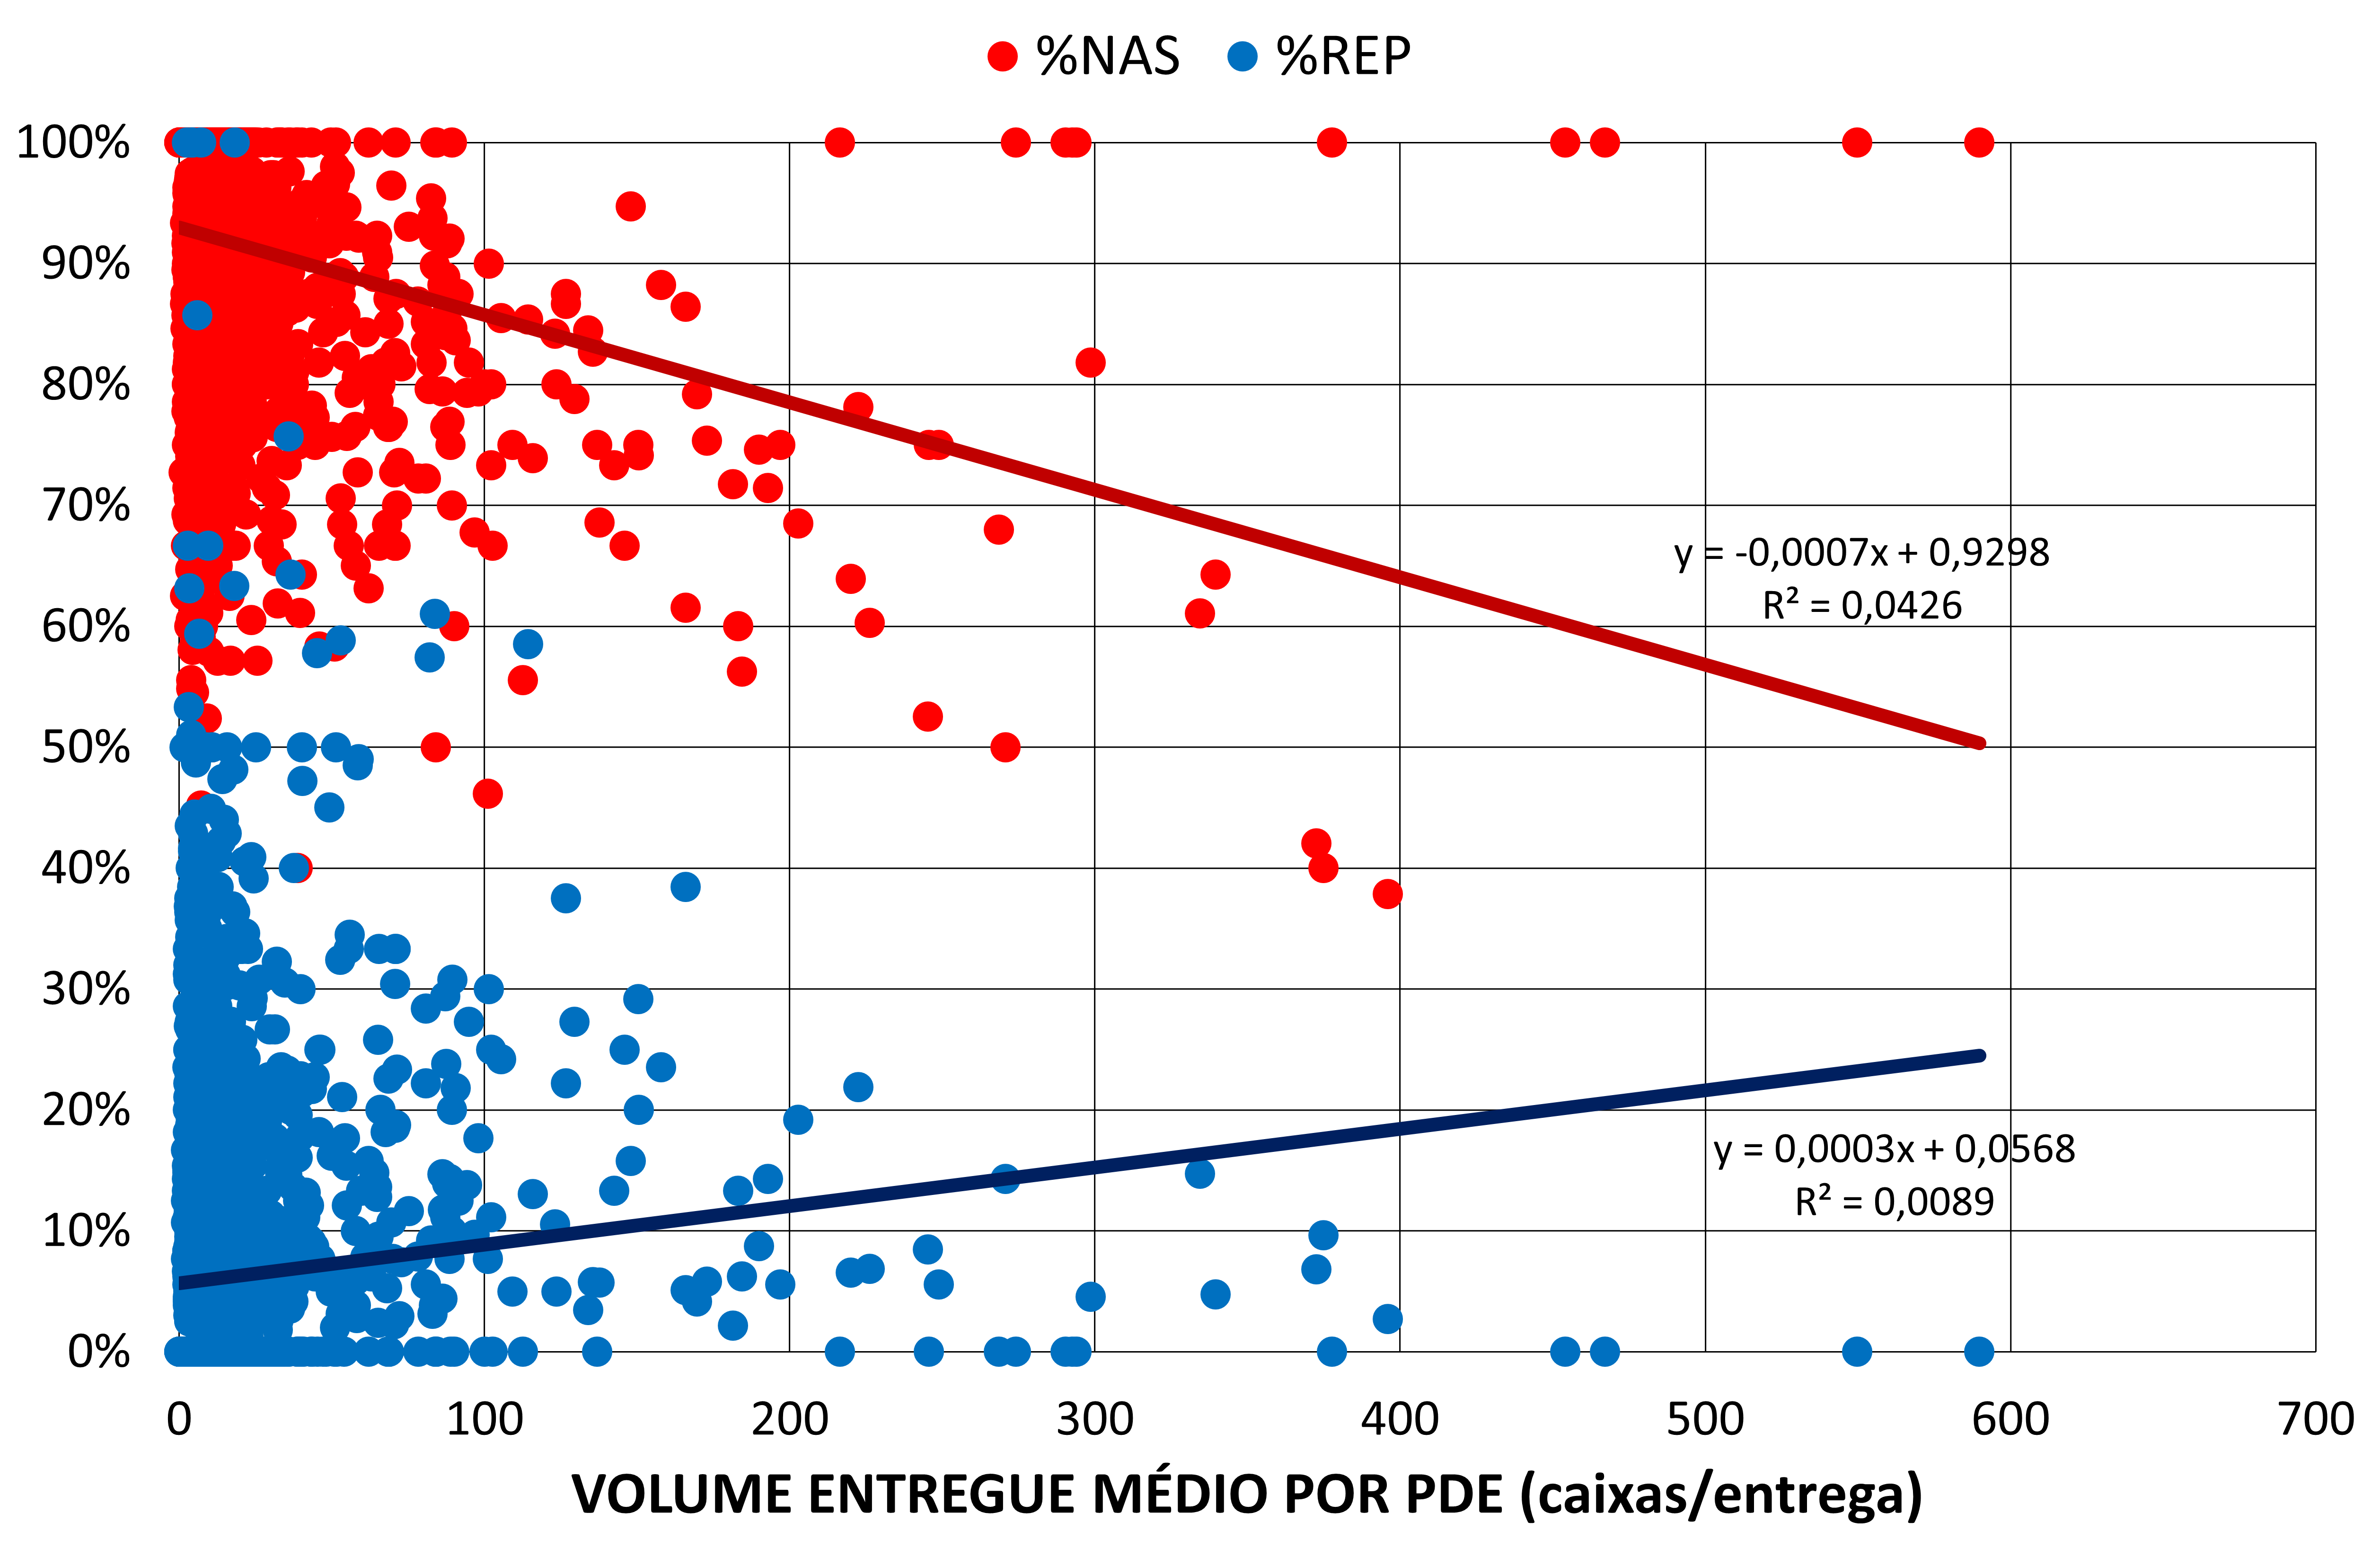
\includegraphics[width=.98\linewidth]{images/5_emp_bebidas/excel_based/Volume.png}
         \label{fig:Volume}
     \end{subfigure}
     \begin{subfigure}{.35\textwidth}
       \centering
       % include second image
       \caption{Estatísticas da Regressão.}
       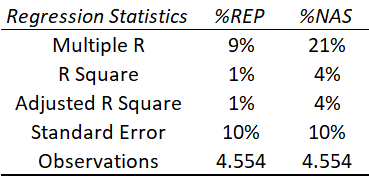
\includegraphics[width=.88\linewidth]{images/5_emp_bebidas/excel_based/Volume_RS.png}
       \label{fig:VolumeRS}
     \end{subfigure}
     \caption*{\ Fonte: Produzido pelos autores Fernandes \& Alves}
\end{figure} % Volume

Observando-se a Figura \ref{fig:Volume} é possível estabelecer que o volume entregue ao PDE tem baixa correlação com os repasses e o NAS. Isso ocorre devido ao alto espalhamento observado dos pontos no gráfico, especialmente em sua porção esquerda, que representa os volumes mais baixos (que são a maioria dos PDE no estudo de caso em questão). Porém, para volumes maiores, é possível observar uma maior padronização na queda de NAS e na queda da ocorrência de repasses, apesar da tendência de regressão dos repasses que é altamente influenciada pelo alto volume de PDE com baixos volumes de entrega com quantidades de repasses percentuais bastante variados.

Tais comportamentos observados para volumes mais altos são coerentes com a concepção de que clientes maiores podem ser tratados com maior cautela pela equipe de entregas, o que leva a uma redução das variáveis-problema.

%%%%%%%%%%%%%%%%%%%%%%%%%%%%%%%%%%%%%%%%%%%%%%%%%%%%%%%%%%%%%%%
\section{Distância entre PDEs e Centro de Distribuição} \label{sec:distanciaCDBebidas}

Em sequência às análises relativas à caracterização da operação da empresa de bebidas, buscou-se identifica-se possíveis efeitos da posição dos PDE nas variáveis problema. Assim, realizou-se a correlação entre os percentuais de repasse, devolução e NAS de cada PDE com sua distância até o CD. 
Foram calculadas as distâncias linear e veicular de todos os PDEs ao CD, considerando toda a base de dados disponível.
Adicionalmente, dispondo-se de ambas as distâncias, calculou-se o fator de circuito para cada par PDE-CD.
Ressalta-se que o processo retrata uma análise preliminar para melhor compreensão das possibilidades de estudo. A posteriori, uma análise mais aprofundada dos efeitos e das diferentes concepções do fator de circuito serão apresentadas na Seção \ref{sec:AMBEV_FC}.

Assim, dispondo-se de todos os indicadores citados, foi possível estabelecer uma correlação entre cada dupla de fatores, conforme ilustrado na Tabela \ref{tab:DistanciaCD_PDEs}, que contém a matriz de correlação entre os diferentes fatores.
Os resultados sugerem que aparentemente não existe uma relação direta entre as variáveis-problema e as distâncias até o CD.
Não obstante, também verifica-se que as três variáveis-problema não possuem relação linear entre si.


\begin{spacing}{1}
\begin{table}[htb] 
    \centering
    \caption{Matriz de correlação entre REP, DEV e NAS e a distância dos PDEs ao CD.}
    \label{tab:DistanciaCD_PDEs}
    % \small
    \begin{tabular}{c|cccccc}
    \hline
    \textit{} & \textit{\%DEV} & \textit{\%NAS} & \textit{\%REP} & \textit{\begin{tabular}[c]{@{}c@{}}Dist Linear\\ CD-PDE\end{tabular}} & \textit{\begin{tabular}[c]{@{}c@{}}Dist Veicular\\ CD-PDE\end{tabular}} & \textit{\begin{tabular}[c]{@{}c@{}}F.C.\\ CD-PDE\end{tabular}} \\ \hline
    \%DEV & \cellcolor[HTML]{63BE7B}1,00 &  &  &  &  &  \\
    \%NAS & \cellcolor[HTML]{FEE883}-0,02 & \cellcolor[HTML]{63BE7B}1,00 &  &  &  &  \\
    \%REP & \cellcolor[HTML]{ECE683}0,11 & \cellcolor[HTML]{FED980}-0,06 & \cellcolor[HTML]{63BE7B}1,00 &  &  &  \\
    Dist Linear CD-PDE & \cellcolor[HTML]{FEE382}-0,04 & \cellcolor[HTML]{EFE784}0,09 & \cellcolor[HTML]{FEDC81}-0,06 & \cellcolor[HTML]{63BE7B}1,00 &  &  \\
    Dist Veicular CD-PDE & \cellcolor[HTML]{FEDC81}-0,06 & \cellcolor[HTML]{EDE683}0,10 & \cellcolor[HTML]{FDD780}-0,07 & \cellcolor[HTML]{71C37C}0,91 & \cellcolor[HTML]{63BE7B}1,00 &  \\
    F.C. CD-PDE & \cellcolor[HTML]{FEE883}-0,03 & \cellcolor[HTML]{FEDE81}-0,05 & \cellcolor[HTML]{FFEB84}-0,02 & \cellcolor[HTML]{F8696B}-0,36 & \cellcolor[HTML]{FCC47C}-0,12 & \cellcolor[HTML]{63BE7B}1,00 \\ \hline
    \end{tabular}
    % \normmalsize
    \caption*{Fonte: Produzido pelos autores Fernandes \& Alves}
\end{table}
\end{spacing}

%%%%%%%%%%%%%%%%%%%%%%%%%%%%%%%%%%%%%%%%%%%%%%%%%%%%%%%%%%%%%%%
\section{Dispersão geográfica das rotas} \label{sec:dispersaoBebidas}

Ainda considerando a posição geográfica dos PDE, busca-se compreender de forma mais ampla como que o conjunto de clientes englobados numa mesma rota podem variar suas taxas de repasse, devolução e NAS a partir de suas dispersões geográficas.

Primeiramente, utilizando o modelo descrito na seção \ref{sec:dispGeoRotas}, calcula-se o conjunto de PDEs considerados ``muito distantes'' dentro de cada rota. 
Isto é, aqueles PDEs que estão localizados fora da ``cauda'' de uma distribuição normal que represente a distribuição das coordenadas dos PDEs, considerando 5\% de significância. 

Em seguida, calculou-se os parâmetros percentuais de repasses, devoluções e NAS para os pontos dentro e fora da região da ``cauda'' e replicou-se o método inteiro para distâncias lineares e veiculares. 
Por fim, os resultados obtidos podem ser observados na Tabela \ref{tab:CompactacaoRotas}, a partir dos quais é possível estabelecer que os PDEs localizados à margem de suas rotas não apresentam resultados consideravelmente distintos daqueles não marginalizados.
Ademais, comparando-se os resultados de ambas distâncias, observa-se pouca variação entre a linear e a veicular.

Em destaque, pode-se considerar a variação no percentual de NAS entre os pontos marginais e os não marginais.
Tal resultado é coerente com a ideia de que a equipe de entrega pode ser mais cautelosa com os PDEs mais distantes de sua rota, devido ao maior consumo de tempo que sua visita exige, evitando-se, assim, alterações da posição sequencial a esmo dos PDEs em questão.

\begin{spacing}{1}
\begin{table}[htb] 
    \centering
    \caption{Resultados da avaliação de PDEs localizados à margem de suas rotas.}
    \label{tab:CompactacaoRotas}
    \begin{tabular}{cccc}
    \hline
    \rowcolor[HTML]{4472C4} 
    \multicolumn{1}{|c|}{\cellcolor[HTML]{548235}{\color[HTML]{FFFFFF} Distância  Linear}} & \multicolumn{1}{c|}{\cellcolor[HTML]{4472C4}{\color[HTML]{FFFFFF} \%REP}} & \multicolumn{1}{c|}{\cellcolor[HTML]{4472C4}{\color[HTML]{FFFFFF} \%DEV}} & \multicolumn{1}{c|}{\cellcolor[HTML]{4472C4}{\color[HTML]{FFFFFF} \%NAS}} \\ \hline
    \multicolumn{1}{|c|}{Fora da Cauda} & \multicolumn{1}{c|}{7\%} & \multicolumn{1}{c|}{2\%} & \multicolumn{1}{c|}{94\%} \\ \hline
    \multicolumn{1}{|c|}{Dentro da Cauda} & \multicolumn{1}{c|}{8\%} & \multicolumn{1}{c|}{1\%} & \multicolumn{1}{c|}{90\%} \\ \hline
    \multicolumn{1}{l}{} & \multicolumn{1}{l}{} & \multicolumn{1}{l}{} & \multicolumn{1}{l}{} \\ \hline
    \rowcolor[HTML]{4472C4} 
    \multicolumn{1}{|c|}{\cellcolor[HTML]{BF8F00}{\color[HTML]{FFFFFF} Distância Veicular}} & \multicolumn{1}{c|}{\cellcolor[HTML]{4472C4}{\color[HTML]{FFFFFF} \%REP}} & \multicolumn{1}{c|}{\cellcolor[HTML]{4472C4}{\color[HTML]{FFFFFF} \%DEV}} & \multicolumn{1}{c|}{\cellcolor[HTML]{4472C4}{\color[HTML]{FFFFFF} \%NAS}} \\ \hline
    \multicolumn{1}{|c|}{Fora da Cauda} & \multicolumn{1}{c|}{7\%} & \multicolumn{1}{c|}{2\%} & \multicolumn{1}{c|}{94\%} \\ \hline
    \multicolumn{1}{|c|}{Dentro da Cauda} & \multicolumn{1}{c|}{8\%} & \multicolumn{1}{c|}{1\%} & \multicolumn{1}{c|}{91\%} \\ \hline
    \end{tabular}
    \caption*{Fonte: Produzido pelos autores Fernandes \& Alves}
\end{table}
\end{spacing}

%%%%%%%%%%%%%%%%%%%%%%%%%%%%%%%%%%%%%%%%%%%%%%%%%%%%%%%%%%%%%%%
\section{Geoestatísticas} \label{sec:geoestatBebidas}

Posteriormente às análises de posicionamento relativo dos PDE, buscou-se, na presente seção, estabelecer um conjunto de análises geoestatísticas a partir da base de dados da empresa de bebidas a fim de se compreender se existe alguma tendência geográfica em ampla escala entre as variáveis-problema estudadas.
Essa análise contemplou apenas a cidade de Guarulhos, que representa 80\% do total de entregas disponíveis na base de dados da empresa de bebidas.

As análises construídas na presente seção são realizadas através da ferramenta GeoDa, cujo uso foi descrito com maiore detalhamento em \ref{GeoDa}. Os conceitos e teorias por trás das análises realizadas, assim como uma apresentação formal dos indicadores representados, pode ser encontrada em \ref{sec:autocorrelacaoEsp}.

Os resultados, que podem ser observados nas Figuras de \ref{fig:AMBEV_LISA_REP} até %, \ref{fig:AMBEV_SCT_REP}, \ref{fig:AMBEV_LISA_DEV}, \ref{fig:AMBEV_SCT_DEV}, \ref{fig:AMBEV_LISA_NAS} e 
\ref{fig:AMBEV_SCT_NAS}, indicam baixa tendência de correlação espacial entre as variáveis estudadas e os bairros da cidade. 
Como observa-se nos três mapas LISA, a maioria dos bairros enquadrou-se como não relevantes (cinza), ou seja, não se pode identificar um padrão espacial na disposição dos clientes que tiveram repasse, devolução ou NAS. 
Este fato é corroborado com o gráfico de dispersão. 
Pode-se observar nos três gráficos apresentados (\ref{fig:AMBEV_SCT_REP}, \ref{fig:AMBEV_SCT_DEV} e \ref{fig:AMBEV_SCT_NAS}) que a correlação estabelecida é numericamente reduzida.

Comparando-se os resultados entre si é possível afirmar que as devoluções e o NAS apresentaram os resultados mais promissores e, nas análises subsequentes, poderão conduzir a resultados mais robustos. 
Tal conclusão é coerente com a percepção de que os repasses podem estar, proporcionalmente, mais associados a comportamentos e decisões dos clientes e da equipe de entregas do que o NAS.% que teve o maior índice de correlação espacial.

\begin{figure}[htb]
     \caption{Correlação espacial do percentual de repasses por bairro.}
     \begin{subfigure}{.49\textwidth}
         \centering
         \caption{Mapa LISA.}
         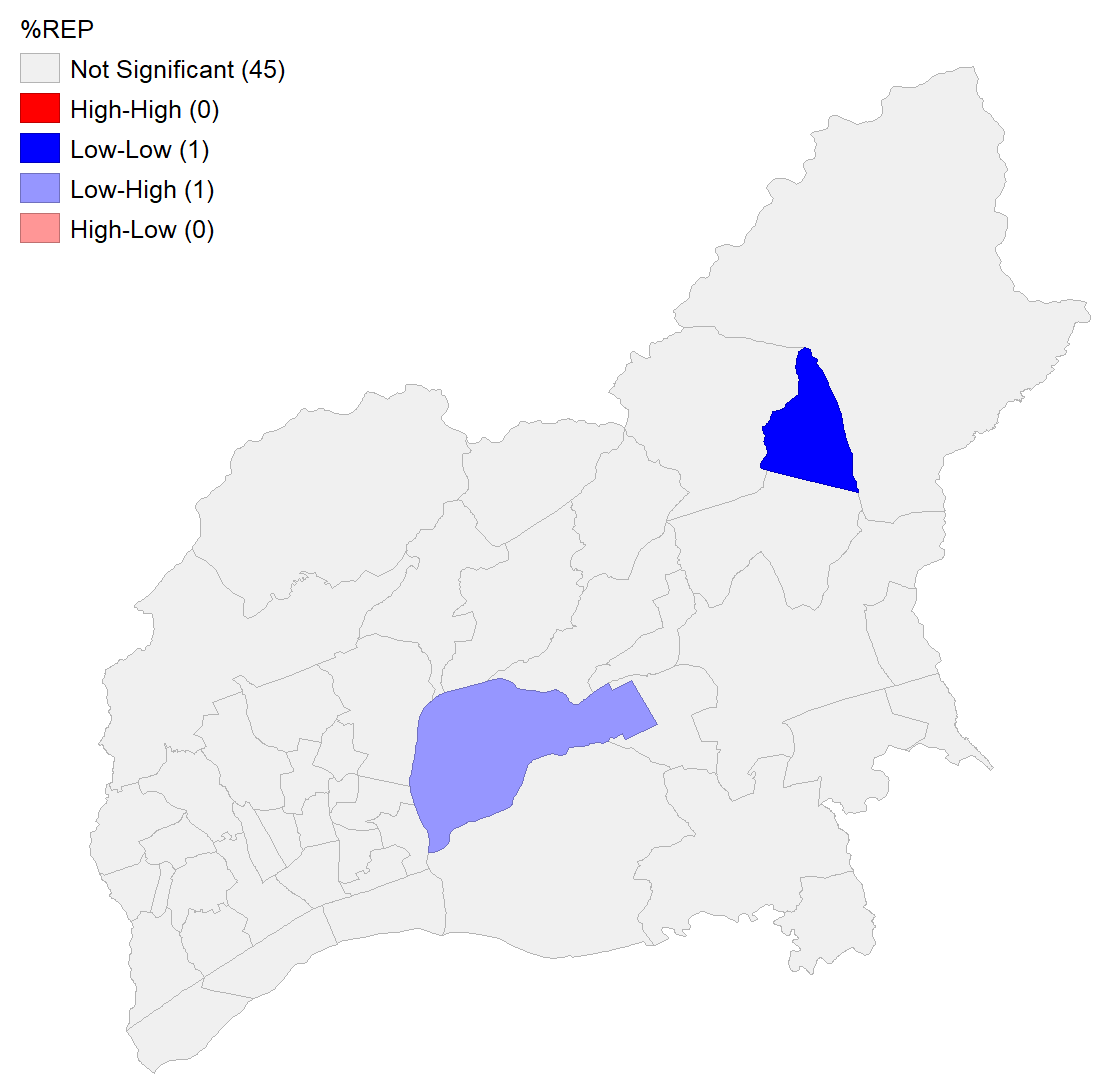
\includegraphics[height=0.75\textwidth]{images/5_emp_bebidas/geoda/BairrosOSM_Corrigidos_REP_lisa.png}
         \label{fig:AMBEV_LISA_REP}
     \end{subfigure}
     \begin{subfigure}{.49\textwidth}
       \centering
       % include second image
       \caption{Gráfico de Dispersão.}
       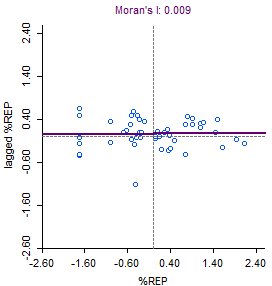
\includegraphics[height=0.75\textwidth]{images/5_emp_bebidas/geoda/BairrosOSM_Corrigidos_REP_sct.png}
       \label{fig:AMBEV_SCT_REP}
     \end{subfigure}
     \caption*{\ Fonte: Produzido pelos autores Fernandes \& Alves}
 \end{figure} % Repasses

\begin{figure}[htb]
     \caption{Correlação espacial do percentual de devoluções por bairro.}
     \begin{subfigure}{.49\textwidth}
         \centering
         % include first image 
         \caption{Mapa LISA.}
         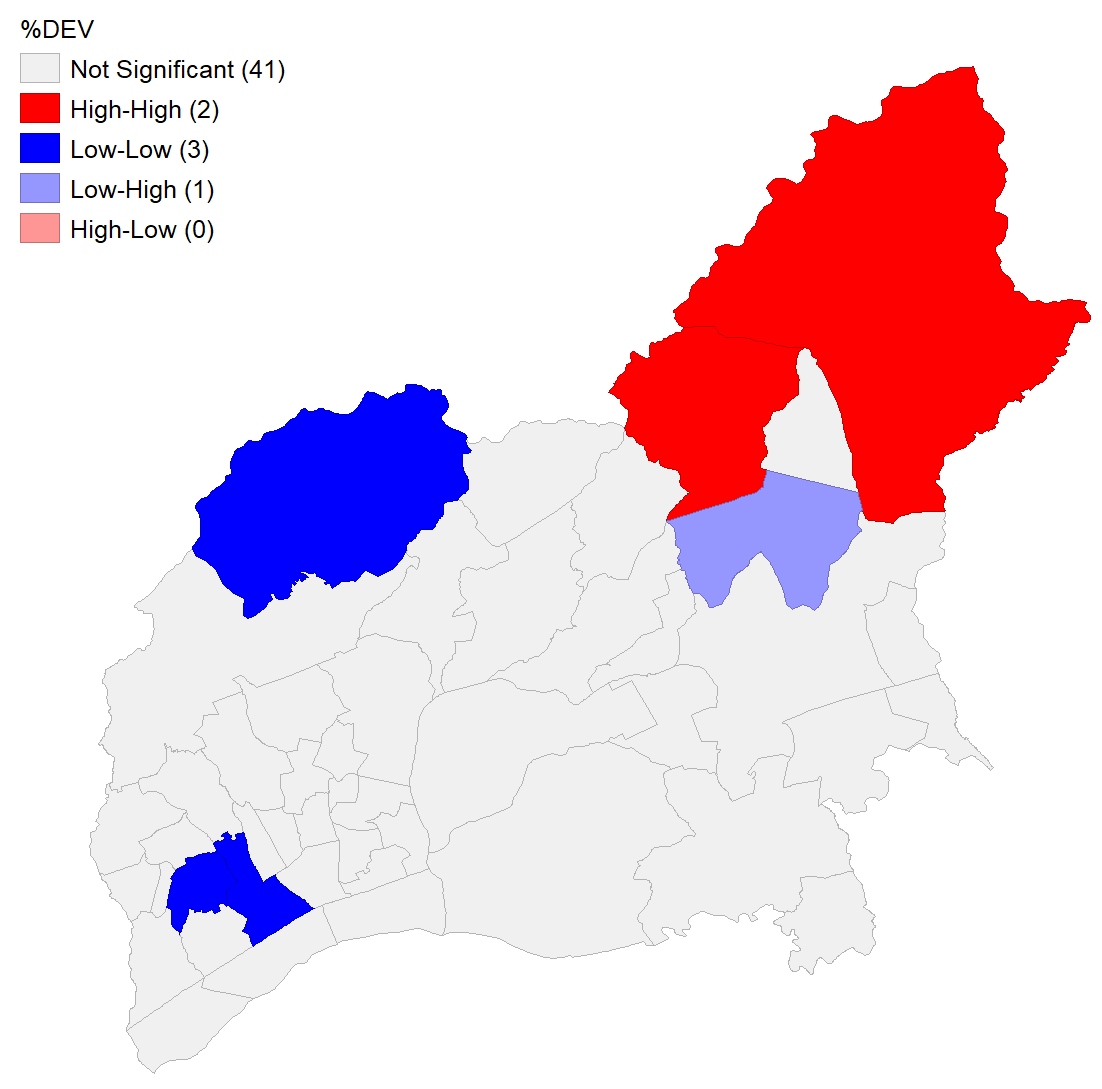
\includegraphics[height=0.75\textwidth]{images/5_emp_bebidas/geoda/BairrosOSM_Corrigidos_DEV_lisa.png}
         \label{fig:AMBEV_LISA_DEV}
     \end{subfigure}
     \begin{subfigure}{.49\textwidth}
       \centering
       % include second image
       \caption{Gráfico de Dispersão.}
       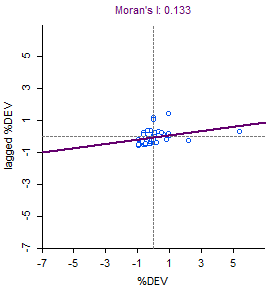
\includegraphics[height=0.75\textwidth]{images/5_emp_bebidas/geoda/BairrosOSM_Corrigidos_DEV_sct.png}
       \label{fig:AMBEV_SCT_DEV}
     \end{subfigure}
     \caption*{\ Fonte: Produzido pelos autores Fernandes \& Alves}
 \end{figure} % Devoluções

\begin{figure}[htb]
     \caption{Correlação espacial do percentual de NAS por bairro.}
     \begin{subfigure}{.49\textwidth}
         \centering
         % include first image 
         \caption{Mapa LISA.}
         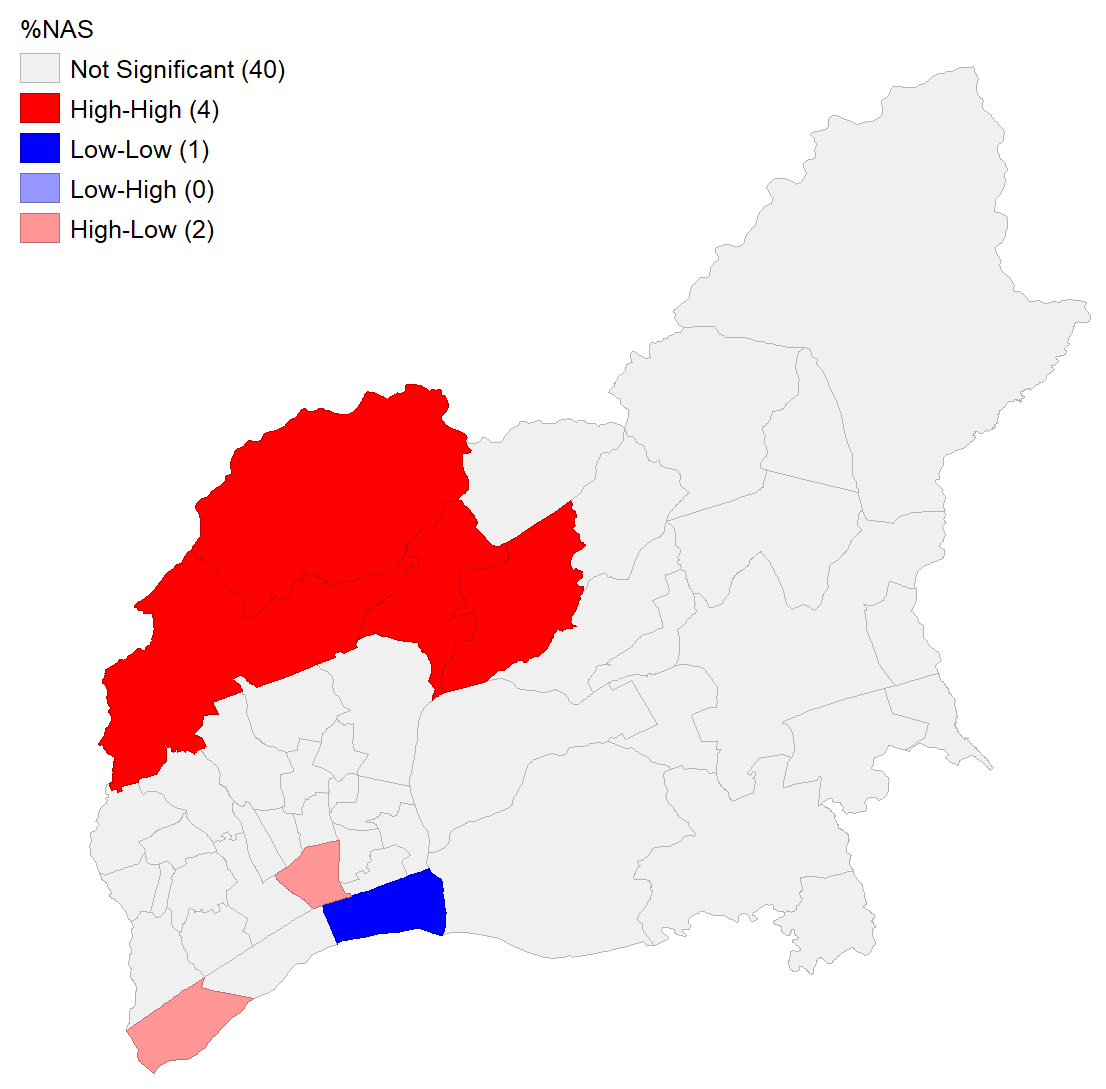
\includegraphics[height=0.75\textwidth]{images/5_emp_bebidas/geoda/BairrosOSM_Corrigidos_NAS_lisa.png}
         \label{fig:AMBEV_LISA_NAS}
     \end{subfigure}
     \begin{subfigure}{.49\textwidth}
       \centering
       % include second image
       \caption{Gráfico de Dispersão.}
       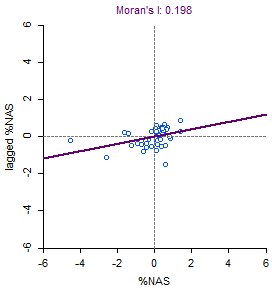
\includegraphics[height=0.75\textwidth]{images/5_emp_bebidas/geoda/BairrosOSM_Corrigidos_NAS_sct.png}
       \label{fig:AMBEV_SCT_NAS}
     \end{subfigure}
     \caption*{\ Fonte: Produzido pelos autores Fernandes \& Alves}
 \end{figure} % NAS

A análise de correlação espacial, porém, não é determinística acerca da possibilidade de haver alguma relação espacial entre os dados, ela se resume, apenas, a um teste de agrupamento entre vizinhos.
Assim, ainda é possível avaliar outros aspectos da localização dos clientes, tal como a influência da estrutura viária dos arredores e das rotas nas variáveis-problema.

%%%%%%%%%%%%%%%%%%%%%%%%%%%%%%%%%%%%%%%%%%%%%%%%%%%%%%%%%%%%%%%
\section{Fator de circuito} \label{sec:AMBEV_FC}

%%%%%%%%%%%%%%%%%%%%%%%%%%%%%%%%%%%%%%%%%%%%%%%%%%%%
\subsection{Validação do modelo}

Antes de partir para o cálculo do fator de circuito envolvendo toda a malha viária estudada, optou-se por selecionar arbitrariamente um PDE que apresentasse alta taxa de repasses e então utilizá-lo como ponto de origem para realização dos cálculos de fator de circuito considerando diferentes pontos ao redor deste PDE e inseridos em um quadrado de lado igual a dois quilômetros.
%
A Figura \ref{fig:FC_1ponto} apresenta o resultado obtido, onde em geral nota-se a presença de uma segmentação dos valores de fator de circuito em relação à região estudada. 
Ou seja, quando o ponto de destino passa a estar localizado em regiões mais ao sudeste da imagem, região essa especialmente separada da parte norte por uma via transversal de grande porte (no caso a Rodovia Presidente Dutra, principal rodovia que atravessa a cidade), os valores de fator de circuito tendem a aumentar.
%

Deste modo fica comprovada a influência que alguns elementos da malha viária podem exercer sobre a medida de fator de circuito, permitindo que as demais análises do trabalho investiguem se essa relação pode ser estendida para medidas tais como a quantidade de repasses e NAS, conforme será apresentado posteriormente.

Para além dos efeitos da Rodovia Presidente Dutra, é interessante que se estabeleça uma visualização mais integrada entre o espaço físico e os resultados de fator de circuito em relação ao ponto em questão.
Para tal, considerou-se a construção de isolinhas - ou linhas de contorno - da medida fator de circuito. 

A Figura \ref{fig:FC_1ponto_iso} apresenta as linhas de contorno em intervalo de 0,5 para o fator de circuito.
É possível evidenciar ainda mais o efeito da rodovia Presidente Dutra sobre os valores de fator de circuito.
Quando observado mais à esquerda, onde há um acesso bem estabelecido, os valores aproximam-se de 3 ao sul da rodovia.
Contudo, na região mais à direita, que conta com menos acessos diretos à rodovia, o valor do fator de circuito pode chegar a 7, novamente ao sul da rodovia. 

Ademais, destaca-se que o fator de circuito nas proximidades do ponto estudado possui valores maiores do que nas extremidades do quadrado analisado, exemplificando o fenômeno descrito pela Equação \ref{eq:limite}. 

Sendo assim, é possível considerar que uma barreira física, como é o caso da rodovia Presidente Dutra, pode apresentar um impacto significativo na ``circuicidade'' da região estudada, reforçando que a geometria da malha viária pode afetar a facilidade de entregas de última milha.

\begin{figure}[H]
    \centering
    \caption{Fator de circuito ao redor de um PDE selecionado}
    \includegraphics[width=0.8\textwidth]{images/5_emp_bebidas/qgis/ResultadoPreliminarQGIS 1.4.pdf}
    \caption*{\ Fonte: Produzido pelos autores Fernandes \& Alves}
    \label{fig:FC_1ponto}
\end{figure}

\begin{figure}[H]
    \centering
    \caption{Isolinhas do fator de circuito ao redor de um PDE selecionado}
    \includegraphics[width=0.8\textwidth]{images/5_emp_bebidas/qgis/ResultadoPreliminarQGIS 1.10.png}
    \caption*{\ Fonte: Produzido pelos autores Fernandes \& Alves}
    \label{fig:FC_1ponto_iso}
\end{figure}

%%%%%%%%%%%%%%%%%%%%%%%%%%%%%%
\subsection{Resultados gerais}

Uma vez evidenciada a interferência entre fator de circuito e malha viária, é possível utilizar dos códigos descritos no capítulo \ref{sec:mat&met} para realizar consultas de distâncias veiculares através do \textit{Google Maps API} e assim avaliar o fator de circuito inserido no contexto da presente pesquisa.

Para realizar os cálculos de fator de circuito, considera-se cada trecho que possa ter sido percorrido por ao menos um veículo. 
Isto inclui os trechos que partem do CD até os PDEs e também os que saem dos PDEs até os PDEs seguintes.
Ao todo, um total de 61.778 trechos tiveram que ser computados em termos de distância euclidiana e veicular, assim como do fator de circuito.
Deste modo, são aplicados os métodos descritos no capítulo \ref{sec:mat&met}, com auxílio da biblioteca \textit{lmr\_analyzer}, os resultados são exportados e puderam então ser analisados.

Tendo posse dos resultados de fator de circuito, foi possível utilizar o \textit{software} QGIS para representar a distribuição espacial dos elementos da matriz de distância, conforme apresentado na Figura \ref{fig:FC_maps2}. 
A Figura mostra o fator de circuito entre diferentes PDEs, filtrados somente aqueles em que a distância não é superior a 500 metros. 
% 
Tal consideração se dá pela relação percebida entre o valor de circuito e a distância real, uma vez que para distâncias grandes o fator de circuito tende a ser cada vez mais próximo de 1.
%
Sendo assim, alternativamente, filtra-se os dados de modo a apresentar somente os casos em que a distância em linha reta entre dois pontos seja de aproximadamente 500 metros, como pode ser visto na Figura . 
%
A distância de 500 metros foi escolhida com base na literatura (\citeauthoronline{AMARAL2020102916}, \citeyear{AMARAL2020102916}). 
%
A Figura \ref{fig:FC_maps3} apresenta um ponto focal da Figura \ref{fig:FC_maps2}. 

\begin{figure}[H]
    \centering
    \caption{Fator de circuito obtido através do \textit{Google Maps} filtrados para distâncias de até 500 metros }
    \includegraphics[width=0.8\textwidth]{images/5_emp_bebidas/qgis/ResultadoPreliminarQGIS 1.6.pdf}
    \caption*{\ Fonte: Produzido pelos autores Fernandes \& Alves}
    \label{fig:FC_maps2}
\end{figure}

\begin{figure}[H]
    \centering
    \caption{Fator de circuito obtido através do \textit{Google Maps} filtrados para distâncias de até 500 metros, com destaque para região próxima ao CD}
    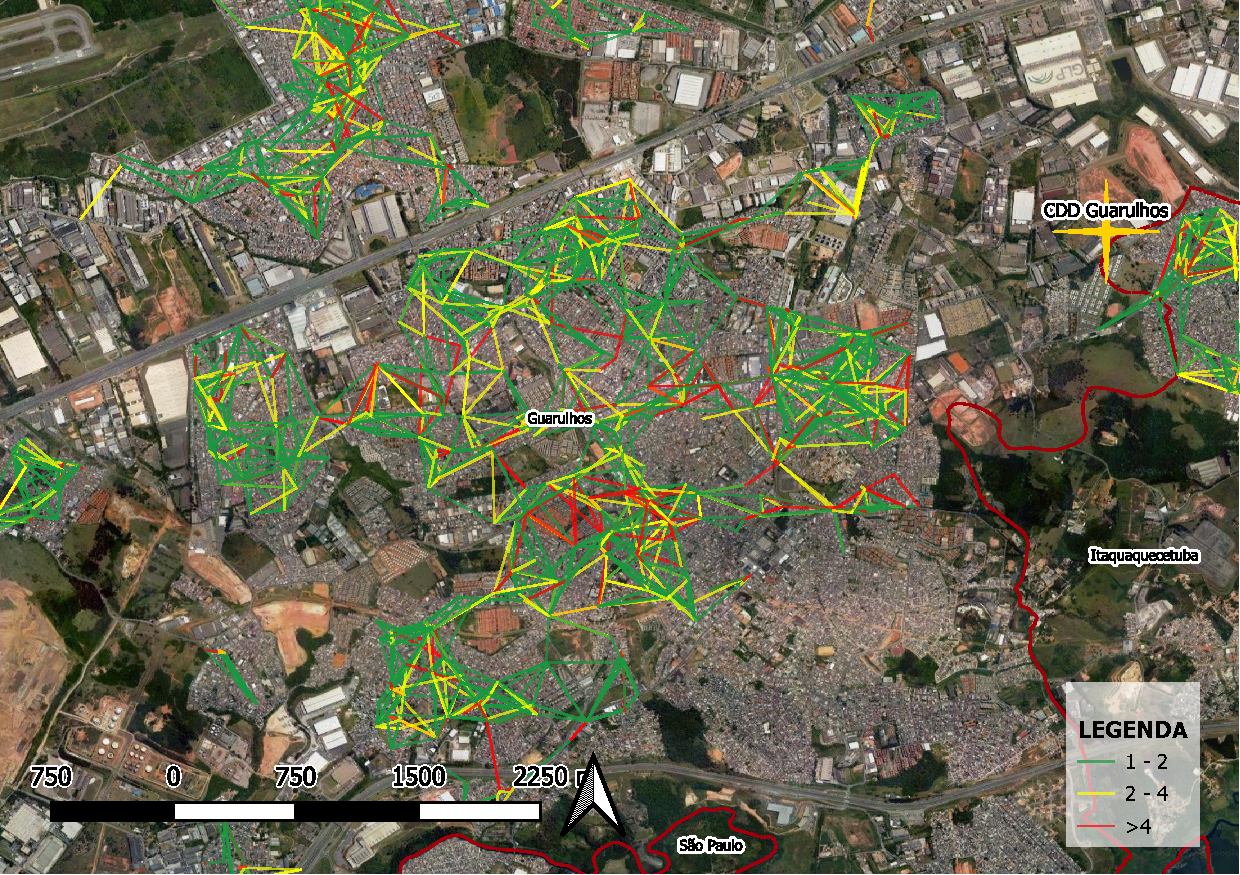
\includegraphics[width=0.8\textwidth]{images/5_emp_bebidas/qgis/ResultadoPreliminarQGIS 1.7.pdf}
    \caption*{\ Fonte: Produzido pelos autores Fernandes \& Alves}
    \label{fig:FC_maps3}
\end{figure}


%%%%%%%%%%%%%%%%%%%%%%%%%%%%%%%%%%%%%%%%%%%%%%%%%%%%%%%%%%%%%%%
\section{Análise da Malha viária} \label{sec:AMBEV_MalhaViaria}

Na presente seção foi descrita a última parte das análises realizadas para o estudo de caso da empresa de bebidas, onde serão aplicados os métodos introduzidos no capítulo \ref{sec:mat&met} para quantificar a topologia da malha viária para cada um dos bairros da cidade de Guarulhos, que é a cidade que compreende a maior região de interesse do estudo (cerca de 80\% da entregadas observadas estão em Guarulhos).
Inicialmente foi testado o modelo para um dos bairros, escolhido aleatoriamente. 
E em seguida foi expandida a análise para todos os demais bairros presentes na cidade.

%%%%%%%%%%%%%%%%%%%%%%%%%%%%%%%%%%%%%%%%%%%%%%%%%%%%%%%%%%
\subsection{Exemplo de aplicação para o bairro de Cumbica}

A partir do arquivo \textit{shapefile} de Guarulhos, utiliza-se um filtro para selecionar apenas o bairro de Cumbica, que será o objeto de estudo desta subseção. 
%
A Figura \ref{fig:Cumbica_network_example} ilustra o conjunto de nós e arcos que representa o bairro de Cumbica, resultado do processo descrito até aqui.
%

Também é possível estudar a problemática de conectividade dos nós da malha conforme descrito por \citeonline{boeing2019urban}, a fim de entender a distribuição espacial da conectividade desses nós.
%
A Figura \ref{fig:network_centrality_cumbica} apresenta o resultado obtido para o bairro de Cumbica, em que os nós mais claros representam uma maior conectividade, ou seja, uma maior quantidade de vias partindo ou chegando dos nós centrais quando comparado com os nós mais periféricos. 

Ademais, as Figuras \ref{fig:Cumbica_bearing_example_histogram} e \ref{fig:Cumbica_bearing_example_polarplot} ilustram o resultado obtido para a análise de orientação de vias - descrita no capítulo \ref{sec:mat&met}, onde cada barra representa um intervalo de $10^{\circ}$.
Em geral nota-se que o bairro de Cumbica tem uma predominância de vias orientadas na direção $50^{\circ}-230^{\circ}$.

Finalmente, é possível gerar e exportar resultados de estatísticas discretas sobre a malha através dos métodos disponíveis na biblioteca \textit{lmr\_analyzier}, já descritos no capítulo \ref{sec:mat&met}.
%
Uma descrição completa das estatísticas obtidas está apresentada no capítulo de apêndice \ref{sec:appResultMalha}, uma vez que consumiriam demasiado tempo de leitura sendo que não são necessariamente cruciais para entendimento do texto. 
Ademais, uma descrição mais resumida dos resultados será apresentada ainda neste capítulo, na seção \ref{sec:relMetricasBebidas}.

Nesta subseção foram calculadas medidas relativas à orientação de vias, conectividade de nós e parâmetros gerais da malha viária de Cumbica, Guarulhos, assim permitindo validar o modelo e testar algumas das ferramentas na prática.
%
Uma vez que se obtém a validação para um dos importantes bairros da amostra de estudo, podendo finalmente prosseguir para a análise global considerando todos os bairros disponíveis. 

\begin{figure}[htb]
    \centering
    \caption{Conjunto de arcos e nós extraídos da malha viária representando o bairro de Cumbica}
    \begin{subfigure}{.46\textwidth}
        \centering
        % include first image 
        \caption{Malha viária - Grafo}
        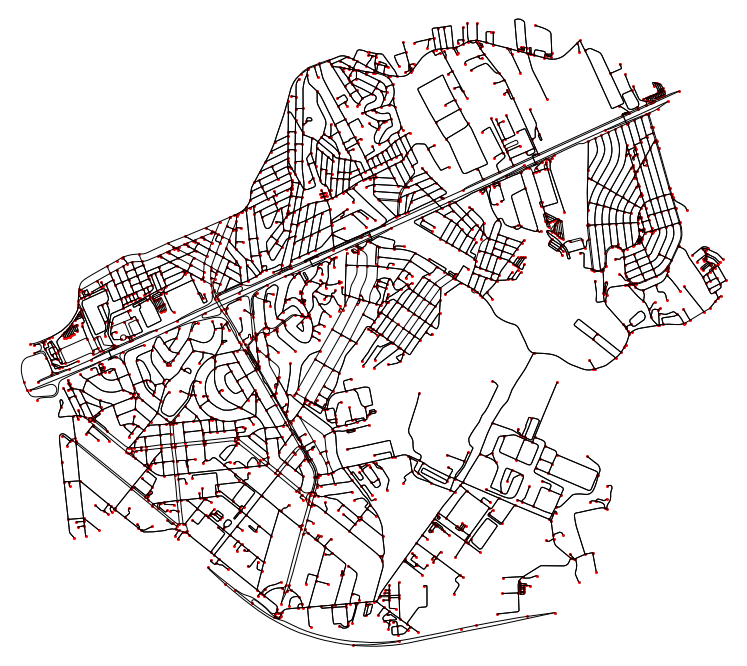
\includegraphics[width=.98\linewidth]{images/5_emp_bebidas/street_network_analysis/cumbica_malha_color.png}
        \label{fig:Cumbica_network_example}
    \end{subfigure}
    \begin{subfigure}{.46\textwidth}
        \centering
        % include second image
        \caption{conectividade dos nós}
        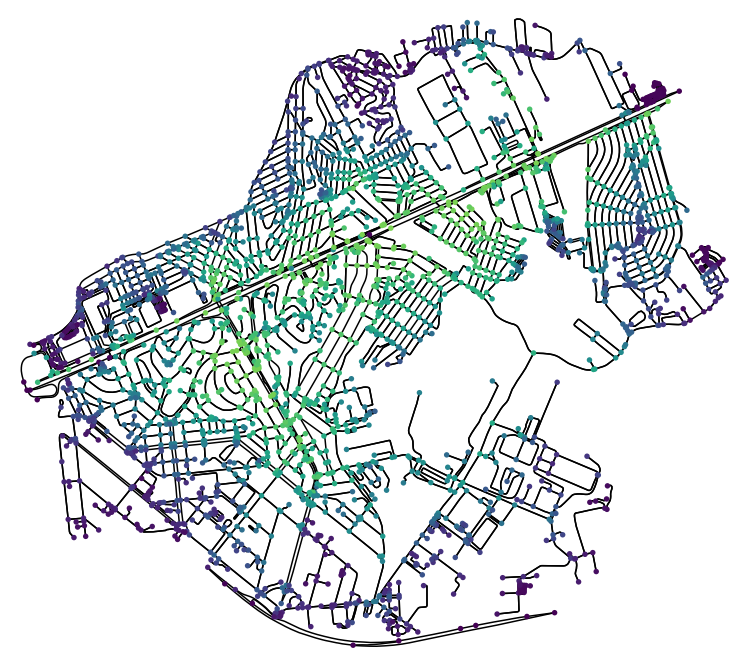
\includegraphics[width=.98\linewidth]{images/5_emp_bebidas/street_network_analysis/network_centrality_cumbica.png}
        \label{fig:network_centrality_cumbica}
    \end{subfigure}
    \caption*{\ Fonte: Produzido pelos autores Fernandes \& Alves}
 \end{figure}

\begin{figure}[htb]
    \centering
    \caption{Histograma de distribuição da orientação de vias de Cumbica - Guarulhos}
    \begin{subfigure}{.45\textwidth}
        \centering
        % include first image 
        \caption{Histograma em projeção linear}
        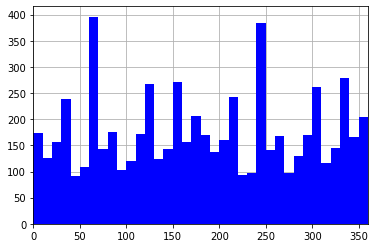
\includegraphics[height=0.6\textwidth]{images/5_emp_bebidas/street_network_analysis/histogram_cumbica.png}
        \label{fig:Cumbica_bearing_example_histogram}
    \end{subfigure}
    \begin{subfigure}{.45\textwidth}
      \centering
      % include second image
      \caption{Histograma em projeção polar}
      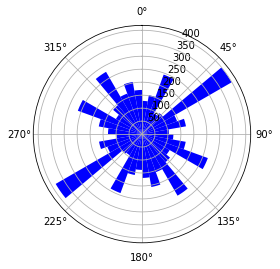
\includegraphics[height=0.6\textwidth]{images/5_emp_bebidas/street_network_analysis/polar_plot_cumbica.png}
      \label{fig:Cumbica_bearing_example_polarplot}
    \end{subfigure}
    \caption*{\ Fonte: Produzido pelos autores Fernandes \& Alves}
\end{figure}

%%%%%%%%%%%%%%%%%%%%%%%%%%%%%%%%%%%%%%%%%%%%%
\subsection{Resultado para os demais bairros}

Começando pelo problema de orientação, utiliza-se uma estrutura de laço do \textit{Python} para iterar sobre os diferentes bairros e realizar os cálculos de orientação um a um, entregando como resultado um histograma de projeção polar que pode ser utilizado posteriormente.
As Figuras \ref{fig:piorbairro_label} e \ref{fig:melhorbairro_label} apresentam exemplos de histogramas polares comparados com a estrutura da malha viária de dois bairros distintos, sendo eles o pior e o melhor cenário em termos de repasses.
Esta comparação permite associar a distribuição de orientações aos valores de repasses, porém curiosamente o bairro que apresentou um dos menores percentuais de repasse é caracterizado por um maior graus de ordenação do arranjo das vias, resultado este que vai na contra-mão da intuição e surpreendeu os autores num primeiro momento.

Por outro lado, a Figura \ref{fig:bearing_bairros} consolida todos histogramas polares em uma única imagem, permitindo uma visualização completa dos resultados.

E finalmente são geradas as estatísticas descritivas para cada um dos bairros, sendo os resultados completos apresentados na Tabela \ref{tab:resultados_completos} do capítulo de apêndice \ref{sec:appResultMalha}, valores estes que podem ser combinados a fim de se investigar existência de alguma correlação entre os valores gerados e os indicadores de repasse e devolução já introduzidos anteriormente. 

\begin{figure}[htb]
    \centering
    % Include first image
    \caption{Resultados para o bairro ``Lavras'', o que representa maior taxa de repasses (11.07\%) e índice de devolução acima da média (5.72\%)}
    \begin{subfigure}{0.42\textwidth}
        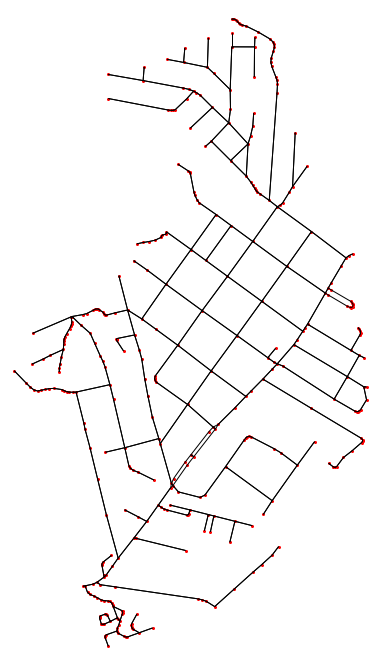
\includegraphics[height=0.75\textwidth]{images/5_emp_bebidas/street_network_analysis/Lavras_malha.png}
    \end{subfigure}
    % Include 2nd image
    \begin{subfigure}{0.42\textwidth}
        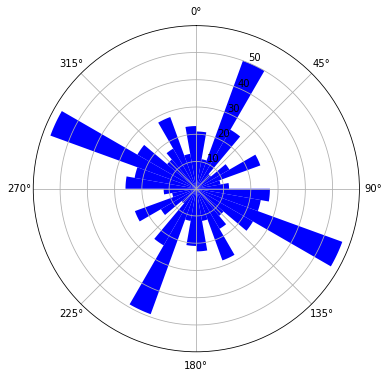
\includegraphics[height=0.75\textwidth]{images/5_emp_bebidas/street_network_analysis/Lavras_polar_plot.png}
    \end{subfigure}
    \caption*{\ Fonte: Produzido pelos autores Fernandes \& Alves}
    \label{fig:piorbairro_label}
\end{figure} % Pior bairro

\begin{figure}[htb]
    \centering
    % Include first image
    \caption{Resultados para o bairro ``Ponte Grande'', o qual apresenta um dos menores índices de repasse (2.44\%) e taxa de devolução abaixo da média (2.03\%)}
    \begin{subfigure}{0.42\textwidth}
        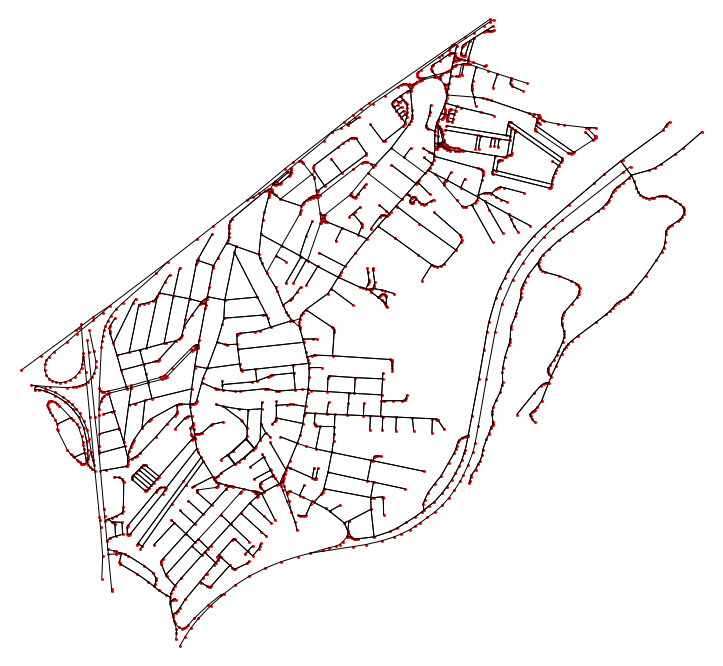
\includegraphics[height=0.75\textwidth]{images/5_emp_bebidas/street_network_analysis/Ponte_grande_malha.png}
    \end{subfigure}
    % Include 2nd image
    \begin{subfigure}{0.42\textwidth}
        \includegraphics[height=0.75\textwidth]{images/5_emp_bebidas/street_network_analysis/ponte_grande_polar_plot.png}
    \end{subfigure}
    \caption*{\ Fonte: Produzido pelos autores Fernandes \& Alves}
    \label{fig:melhorbairro_label}
\end{figure} % Melhor bairro

%%%%%%%%%%%%%%%%%%%%%%%%%%%%%%%%%%%%%%%%%%%%%%%%%%%%%%%%%%%%%%%
\section{Relação entre as medidas estudadas} \label{sec:relMetricasBebidas}

Na presente seção, busca-se apresentar os resultados finais de corrrelação das variáveis-problema com os indicadores de malha e de fator de circuito apresentados nas seções anteriores. Assim, na Subseção \ref{FC_repBebidas}, é apresentada a análise de correlação do fator de circuito com o repasse. Já na Subseção \ref{ImpactoMalhaViariaBebidas}, é apresentada a análise dos resultados de correlação obtidos entre os indicadores da estrutura viária com os repasses e as devoluções.

%%%%%%%%%%%%%%%%%%%%%%%%%%%%%%%%%%%%%%%%%%%%%%%%%%%
\subsection{Fator de circuito e repasses} \label{FC_repBebidas}

A partir dos dados de fator de circuito calculados na Seção \ref{sec:AMBEV_FC}, é possível gerar um comparativo entre eles e os repasses. O objetivo da presente subseção é avaliar o efeito que o fator de circuito pode ter sobre a operação da empresa de bebidas brasileira a partir da perspectiva dos repasses.

Para a quantidade de repasses, os PDEs foram agrupados por bairros, ou seja, foi estudada a média do fator de circuito em relação ao total de repasses consolidado por bairros. 
%
Essa alternativa se mostrou eficaz para aliviar as discrepâncias entre os valores de repasse apresentados pelos mais de 4.000 PDEs.
%
A Figura \ref{fig:FC_repasse} apresenta a correlação obtida.
%
É possível observar no gráfico um certo grau de espalhamento dos pontos em suas relações de repasse e Fator de Circuito. 
Apesar da curva de tendência apresentada, identifica-se a presença de um ponto muito distante dos demais (\textit{outlier}), o que contribui significativamente para a tendência positiva da reta.

\begin{figure}[htb]
    \centering
    \caption{Correlação entre quantidade de repasses e fator de circuito médio por bairro}
    \includegraphics[width=0.8\textwidth]{images/5_emp_bebidas/excel_based/FC_bairros_novo.png}
    \caption*{\ Fonte: Produzido pelos autores Fernandes \& Alves}
    \label{fig:FC_repasse}
\end{figure}


%%%%%%%%%%%%%%%%%%%%%%%%%%%%%%%%%%%%
\subsection{Impacto da malha viária} \label{ImpactoMalhaViariaBebidas}

Em sequência, busca-se avaliar, para além do fator de circuito, como que os indicadores da estrutura viária obtidos na Seção \ref{sec:AMBEV_MalhaViaria} relacionam-se com os repasses e as devoluções do estudo de caso a partir do conceito de correlação linear simples, apresentado na Seção \ref{RegressoesLineares}.

Para tal, a Tabela \ref{tab:correlacao}, presente nos apêndices, apresenta os coeficientes de correlação de Pearson entre as principais variáveis obtidas no problema.
Nela, é possível extrair que as principais variáveis explicativas da quantidade de repasses por bairro são o comprimento total de vias naquele bairro e a quantidade de nós e de arcos, bem como a quantidade de intersecções.
Estas variáveis também explicam bem os valores de caixas devolvidas, que neste caso representa a devolução total por bairro.
Contudo nota-se que as correlações são mais fortes quando se analisam valores absolutos de devoluções e repasses por bairro em vez de valores relativos ou normalizados.

Nesse sentido, os resultados obtidos através da abordagem adotada sugerem que as principais variáveis explicativas do total de caixas devolvidas por bairro seriam o comprimento total de vias ($r=0,851$), número total de arcos ($r=0,787$), número total de nós ($r=0,770$) e quantidade total de intersecções ($r=0,767$), nesta ordem.
Todos estes valores positivos de coeficiente de regressão indicam uma tendência de haver maior quantidade de devoluções conforme se aumenta a complexidade da malha, representada pela quantidade total de seus elementos.
Já quanto à quantidade de repasses por bairros, obtém-se conclusões análogas.

Infelizmente o parâmetro $k\_average$, que representa a média de ângulos de incidência dos arcos sobre os nós, não apresentou nenhuma correlação consideravelmente alta em relação aos outros atributos estudados, o que pode ser de certa forma compreendido também pelos resultados apresentados nas Figuras \ref{fig:piorbairro_label} e \ref{fig:melhorbairro_label}. 
Havia uma expectativa de um comportamento correlato entre o indicador e as variáveis-problema estudadas devido ao estudo realizado para com os radares direcionais das vias de cada bairro. O parâmetro $k\_average$, porém, é uma representação bastante limitada dos radares direcionais, por retratar a média, somente, e não o comportamento de espalhamento dos mesmos.

\chapter{Estudo de caso II: Amazon} \label{sec:EstCasoAmazon}

Ao longo do presente Capítulo serão descritos os resultados obtidos para o caso da Amazon.
Primeiro são apresentadas informações gerais sobre as rotas analisadas, assim como sobre as cidades em que estão localizadas.
Em seguida apresenta-se os resultados de geoestatística, análise do fator de circuito e quantificação da geometria das malhas viárias.
Por último, está apresentada a relação entre as diferentes variáveis geradas, incluindo resultado de regressões lineares simples e múltiplas.

%%%%%%%%%%%%%%%%%%%%%%%%%%%%%%%%%%%%%%%%%%%%%%%%%%%%%%%%%%%%%%%%%%
\section{Localização geográfica} \label{sec:loc_geografica_amazon}

Ao todo foram analisadas cinco regiões metropolitanas, que correspondem às seguintes cidades americanas: Austin (TX), Boston (MT), Chicago (IL), Los Angeles (CA) e Seattle (WA).
Cada uma dessas regiões conta com mais de um centro de distribuição, dos quais partiram as 6112 rotas que estão registradas na base de dados, conforme pode ser observado na Tabela \ref{tab:resumo_entregas}.
Nota-se que maior parte das rotas (cerca de 45\%) está localizada na cidade de Los Angeles e que cada rota contém em média 148 entregas $\left( 148 = \frac{904517}{6112} \right)$.

\singlespacing
\begin{table}[H]
    \caption{Número de CDs, rotas e entregas por cidade}
    \label{tab:resumo_entregas}
    \centering
    \begin{tabular}{|ccccc|}
        \hline
        \textbf{Cidade} &
        \textbf{Centros de Distribuição} &
        \textbf{Rotas} &
        \textbf{Entregas} &
        \textbf{\% do total}\\ \hline
        Austin         & 1  & 220  &  31274 & 3.5 \\
        Boston         & 3  & 931  & 140622 & 15.5\\
        Chicago        & 4  & 1004 & 162410 & 18.0\\
        Los Angeles    & 6  & 2876 & 414440 & 45.8\\
        Seattle        & 3  & 1081 & 155771 & 17.2\\ \hline
        \textbf{Total} & 17 & 6112 & 904517 & 100\\ \hline
    \end{tabular}
    \caption*{\ Fonte: Produzido pelos autores Fernandes \& Alves}
\end{table}
\onehalfspacing

A Figura \ref{fig:amazon_locations} apresenta a distribuição espacial dos centros de distribuição (CDs) e pontos de entrega estudados (PDEs) em cada uma das cinco cidades.
Nota-se que muitas das entregas foram realizadas em localidades fora da cidade principal, ou seja, em regiões suburbanas.
Dessa forma, apenas parte das rotas será analisada, de modo que os resultados obtidos sejam compatíveis com a quantificação de malha viária.
A Tabela \ref{tab:mantidos_amazon} apresenta o percentual de rotas que serão mantidas no estudo de cada uma das cidades, no geral, destaca-se que cerca de $28\%$ das rotas serão analisadas.

\begin{figure}[H]
    \centering
    \caption{Distribuição espacial das cinco operações estudadas (\textit{Amazon})}
    \label{fig:amazon_locations}
    \begin{subfigure}{.32\textwidth}
        \caption{Austin}
        \includegraphics[width=\textwidth]{images/6_amazon/locations/austin_locations.png}
    \end{subfigure}
    %
    \begin{subfigure}{.32\textwidth}
        \caption{Boston}
        \includegraphics[width=\textwidth]{images/6_amazon/locations/boston_locations.png}
    \end{subfigure}
    %
    \begin{subfigure}{.32\textwidth}
        \caption{Chicago}
        \includegraphics[width=\textwidth]{images/6_amazon/locations/chicago_locations.png}
    \end{subfigure}
    %
    \begin{subfigure}{.32\textwidth}
        \caption{Los Angeles}
        \includegraphics[width=\textwidth]{images/6_amazon/locations/los_angeles_locations.png}
    \end{subfigure}
    %
    \begin{subfigure}{.32\textwidth}
        \caption{Seattle}
        \includegraphics[width=\textwidth]{images/6_amazon/locations/seattle_locations.png}
    \end{subfigure}
    \caption*{\ Fonte: Produzido pelos autores Fernandes \& Alves}
\end{figure}

\singlespacing
\begin{table}[H]
    \centering
    \caption{Percentual de entregas estudadas em relação ao total (Amazon)}
    \label{tab:mantidos_amazon}
    \begin{tabular}{|c|ccc|}
    \hline
    \multicolumn{1}{|c|}{\textbf{Cidade}} & \multicolumn{1}{c|}{\textbf{Entregas Totais}} & \multicolumn{1}{c|}{\textbf{Entregas Estudadas}} & \textbf{\% do total} \\ \hline
    Austin & 31274 & 10000 & 32 \\
    Boston & 140622 & 37283 & 27 \\
    Chicago & 162410 & 26280 & 16 \\
    Los Angeles & 414440 & 144411 & 35 \\
    Seattle & 155771 & 34276 & 22 \\ \hline
    \textbf{Total} & 904517 & 252250 & 28 \\ \hline
    \end{tabular}
    \caption*{\ Fonte: Produzido pelos autores Fernandes \& Alves}
\end{table}
\onehalfspacing

%%%%%%%%%%%%%%%%%%%%%%%%%%%%%%%%%%%
\section{Descrição temporal}

A base de dados disponibilizada contempla um total de trinta e oito dias de operação de entregas da \textit{Amazon}, contudo, este valor varia de acordo com a cidade analisada, conforme pode ser observado na tabela \ref{tab:timesAmazon}.
%
\begin{table}[H]
    \centering
    \caption{Intervalo de tempo observado em de cada cidade (\textit{Amazon})} \label{tab:timesAmazon}
    \begin{tabular}{|cccc|}
        \hline
        \textbf{Cidade} & \textbf{Início} & \textbf{Fim} & \textbf{Dias} \\ \hline
        Austin          & 20-Jul-18       & 17-Aug-18    & 28            \\
        Boston          & 20-Jul-18       & 17-Aug-18    & 28            \\
        Chicago         & 19-Jul-18       & 17-Aug-18    & 29            \\
        Los Angeles     & 19-Jul-18       & 26-Aug-18    & 38            \\
        Seattle         & 19-Jul-18       & 26-Aug-18    & 38            \\ \hline
        \textbf{Total}  & 19-Jul-18       & 26-Aug-18    & 38            \\ \hline
    \end{tabular}
    \caption*{Fonte: Produzido pelos autores Fernandes \& Alves}
\end{table}
%
A Figura \ref{fig:amazon_times} apresenta a distribuição do número de entregas realizadas em cada uma das cidades ao longo do tempo.
Destaca-se que a cidade de Los Angeles apresenta a maior taxa de entregas diárias dentre as cidades analisadas, atingindo mais de $20000$ (vinte mil) entregas em um dos dias observados. 
Contudo, inexplicavelmente, há uma queda no número de entregas a partir do dia 18 de agosto de 2018.
Por outro lado, Austin tem a menor taxa de entregas diária, apesar de apresentar valores mais regulares ao longo do tempo.
%
\begin{figure}[H]
    \centering
    \caption{Distribuição temporal de entregas nas cinco operações estudadas (Amazon)}
    \label{fig:amazon_times}
    \begin{subfigure}{.45\textwidth}
        % \caption{Austin}
        \includegraphics[width=\textwidth]{images/6_amazon/times/austin_deliveries_times.pdf}
    \end{subfigure}
    %
    \begin{subfigure}{.45\textwidth}
        % \caption{Boston}
        \includegraphics[width=\textwidth]{images/6_amazon/times/boston_deliveries_times.pdf}
    \end{subfigure}
    %
    \begin{subfigure}{.45\textwidth}
        % \caption{Chicago}
        \includegraphics[width=\textwidth]{images/6_amazon/times/chicago_deliveries_times.pdf}
    \end{subfigure}
    %
    \begin{subfigure}{.45\textwidth}
        % \caption{Los Angeles}
        \includegraphics[width=\textwidth]{images/6_amazon/times/la_deliveries_times.pdf}
    \end{subfigure}
    %
    \begin{subfigure}{.45\textwidth}
        % \caption{Seattle}
        \includegraphics[width=\textwidth]{images/6_amazon/times/seattle_deliveries_times.pdf}
    \end{subfigure}
    \caption*{Fonte: Produzido pelos autores Fernandes \& Alves}
\end{figure}


%%%%%%%%%%%%%%%%%%%%%%%%%%%%%%%%%%%%%%%%%%%%%%%%%%%%%%%%%%
\section{Quantidade de Entregas, Repasses e Devoluções}

Conforme já mencionado na Seção \ref{sec:loc_geografica_amazon}, um total de 6112 rotas estão disponíveis na base de dados estudada.
Cada rota é composta por diferentes PDEs e cada PDE recebe uma certa quantidade de pacotes.
O percentual de repasses e devoluções foi calculado em relação ao número de pacotes, em vez de se calcular em relação ao número de entregas, como foi feito no caso da empresa de bebidas. 
Este método de cálculo é justificado pelo fato de as entregas da \textit{Amazon} permitirem que parte dos pacotes de uma entrega seja devolvida e outra parte entregue.
Dessa forma, estes percentuais tendem a ser relativamente menores do que os apresentados no estudo de caso anterior. 

A contagem do número de rotas em cada uma das cinco cidades pode ser vista na Tabela \ref{tab:resumo_dev_rep_Amazon}, assim como o percentual de repasse e devolução apresentado por cada uma das cidades.
A partir das informações, pode-se destacar que apenas $0.075\%$ dos pacotes foram repassados, sendo que a cidade de Los Angeles possui a taxa de repasses mais elevada dentre as cinco cidades e apenas $0.002\%$ dos pacotes foram devolvidos.

\singlespacing
\begin{table}[H]
    \caption{Entregas, devoluções e repasses por cidade (\textit{Amazon})}
    \label{tab:resumo_dev_rep_Amazon}
    \centering
    \begin{tabular}{|ccc|}
        \hline
        \textbf{Cidade} &
          \textbf{Repasse (\%)} &
          \textbf{Devolução (\%)} \\ \hline
            Austin         & 0.593 & 0.004 \\
            Boston         & 0.553 & 0.000 \\
            Chicago        & 0.545 & 0.003 \\
            Los Angeles    & 0.933 & 0.003 \\
            Seattle        & 0.679 & 0.002 \\ \hline
            \textbf{Total} & \textbf{0.749} & \textbf{0.002} \\ \hline
    \end{tabular}
    \caption*{\ Fonte: Produzido pelos autores Fernandes \& Alves}
\end{table}
\onehalfspacing

A Figura \ref{fig:heatmapAmazon1} apresenta a distribuição espacial de pacotes entregues e pacotes repassados na cidade de Los Angeles. Cita-se que a partir da presente seção, as análises apresentadas serão realizadas a partir dos resultados obtidos no município de Los Angeles. Isso se dá pela maior representatividade que a cidade tem no operação da empresa, além de apresentar maiores índices de repasses. As análises das outras cidades podem ser encontradas na biblioteca pública de códigos da pesquisa, apresentada na bibliografia.
É possível notar uma concentração (ou foco) de repasses na região central da cidade, assim como uma concentração de pacotes entregues também na região central.
Contudo a região de concentração de entregas não é exatamente igual à região de concentração de repasses, o que sugere que provavelmente a região de maior incidência de repasses possui alguma característica - por exemplo, organização da malha viária - que a deixa mais propícia a apresentar rotas com repasses.

\begin{figure}[htb]
    \centering
    \caption{Mapa de calor de entregas e repasses na cidade de Los Angeles (\textit{Amazon})} \label{fig:heatmapAmazon1}
    \begin{subfigure}{0.49\textwidth}
        \caption{Pacotes entregues}
        \includegraphics[width=\textwidth]{images/6_amazon/rep_e_dev/los_angeles_entregas.png}
    \end{subfigure}
    \begin{subfigure}{0.49\textwidth}
        \caption{Pacotes repassados}
        \includegraphics[width=\textwidth]{images/6_amazon/rep_e_dev/los_angeles_failed.png}
    \end{subfigure}
    \caption*{\ Fonte: Produzido pelos autores Fernandes \& Alves}
\end{figure}

A Figura \ref{fig:devolucoes_LA} apresenta a distribuição espacial do número de pacotes devolvidos na cidade de Los Angeles.
Os bairros que apresentam o maior número de devoluções são ``Sherman Oaks'' e ``Hollywood Hills''.
Destaca-se que, mesmo nestes bairros mais problemáticos, apenas dois pacotes foram devolvidos em todas as rotas observadas.

\begin{figure}[H]
    \centering
    \caption{Pacotes devolvidos por bairros da cidade de Los Angeles (\textit{Amazon})}
    \label{fig:devolucoes_LA}
    \includegraphics[width=0.7\textwidth]{images/6_amazon/rep_e_dev/los_angeles_rejected.png}
    \caption*{\ Fonte: Produzido pelos autores Fernandes \& Alves}
\end{figure}


%%%%%%%%%%%%%%%%%%%%%%%%%
\section{Geoestatísticas} \label{sec:Amazon_AnalisesPreliminares}

Nas Figuras \ref{fig:AMAZON_LISA_REP} e \ref{fig:AMAZON_LISA_DEV} é possível observar os mapas LISA construídos para a cidade de Los Angeles considerando, respectivamente, os valores de repasse e devolução calculados para cada bairro. 
Ademais, as Figuras \ref{fig:AMAZON_SCT_REP} e \ref{fig:AMAZON_SCT_DEV} indicam numericamente a correlação espacial. 

\begin{figure}[H]
    \centering
     \caption{Correlação espacial do percentual de repasses por bairro (\textit{Amazon})}
     \begin{subfigure}{.45\textwidth}
         \centering
         % include first image 
         \caption{Mapa LISA.}
         \includegraphics[height=0.75\textwidth]{images/6_amazon/geoda/BairrosLA_REP_lisa.png}
         \label{fig:AMAZON_LISA_REP}
     \end{subfigure}
     \begin{subfigure}{.45\textwidth}
       \centering
       % include second image
       \caption{Gráfico de Dispersão.}
       \includegraphics[height=0.75\textwidth]{images/6_amazon/geoda/BairrosLA_REP_scatter.png}
       \label{fig:AMAZON_SCT_REP}
     \end{subfigure}
     \caption*{\ Fonte: Produzido pelos autores Fernandes \& Alves}
 \end{figure} % Repasses

\begin{figure}[H]
    \centering
     \caption{Correlação espacial do percentual de devoluções por bairro (\textit{Amazon})}
     \begin{subfigure}{.45\textwidth}
         \centering
         % include first image 
         \caption{Mapa LISA}
         \includegraphics[height=0.75\textwidth]{images/6_amazon/geoda/BairrosLA_DEV_lisa.png}
         \label{fig:AMAZON_LISA_DEV}
     \end{subfigure}
     \begin{subfigure}{.45\textwidth}
       \centering
       % include second image
       \caption{Gráfico de Dispersão.}
       \includegraphics[height=0.75\textwidth]{images/6_amazon/geoda/BairrosLA_DEV_scatter.png}
       \label{fig:AMAZON_SCT_DEV}
     \end{subfigure}
     \caption*{\ Fonte: Produzido pelos autores Fernandes \& Alves}
 \end{figure} % Devoluções

As análises geoestatísticas, de modo geral, apresentaram baixo nível de correlação espacial nos bairros de Los Angeles considerando indicadores de repasse e devolução percentuais. 
A alta ocorrência de bairros classificados como ``LOW-LOW'' no mapa LISA de devoluções percentuais decorre do baixíssimo nível de ocorrência de devoluções na base, o que implica num número alto de bairros com 0\% de devoluções. 

Estes resultados, porém, não eliminam as possibilidades de a geografia dos bairros influenciarem a ocorrência de repasses e devoluções. 
Os resultados representam apenas tendências entre bairros vizinhos. 
Assim, bairros que estejam localizados em regiões distintas da cidade não são comparadores entre si. 
Portanto, nos tópicos seguintes serão analisadas com maiores detalhes as variáveis de repasse de devolução considerando características individuais de cada bairro.

%%%%%%%%%%%%%%%%%%%%%%%%%%%%%%%%%%%%%%%%%%%%%%%%%
\section{Fator de circuito} \label{sec:Amazon_FC}

A fim de se calcular o fator de circuito das rotas analisadas, para cada rota foram somadas as distâncias euclidianas entre os diferentes pontos de entregas, assim como as distâncias veiculares.
A média das distâncias totais das rotas é apresentada na Figura \ref{fig:distanciasRotasLA}, onde estão resumidas por bairros.
É possível identificar que bairros que estão mais distantes dos CDs tendem a conter rotas de maiores distâncias totais, o que é condizente com a estrutura urbana onde se encontram regiões mais densas em áreas centrais da cidade. 
Assim, o veículo realiza maiores deslocamentos para acessar os clientes mais dispersos.

\begin{figure}[H]
    \centering
    \caption{Média de distâncias totais de rotas na cidade de Los Angeles (\textit{Amazon})} \label{fig:distanciasRotasLA}
    \begin{subfigure}{0.45\textwidth}
        \caption{Distância Euclidiana}
        \includegraphics[width=\textwidth]{images/6_amazon/distancias/Avg Sum of Euc. Dist. Route - LA.png}
    \end{subfigure}
    \begin{subfigure}{0.45\textwidth}
        \caption{Distância veicular}
        \includegraphics[width=\textwidth]{images/6_amazon/distancias/Avg Sum of Driving Dist. Route - LA.png}
    \end{subfigure}
    \caption*{\ Fonte: Produzido pelos autores Fernandes \& Alves}
\end{figure}

A Figura \ref{fig:fc_medio_LA} apresenta os valores médios de fator de circuito por bairros de Los Angeles.
A princípio, não é possível identificar qualquer padrão ou consistência na distribuição espacial apresentada

\begin{figure}[H]
    \centering
    \caption{Fator de circuito médio nos bairros de Los Angeles (\textit{Amazon})}
    \label{fig:fc_medio_LA}
    \includegraphics[width=0.55\textwidth]{images/6_amazon/fc/fc_la_avvg_per_stop.png}
    \caption*{\ Fonte: Produzido pelos autores Fernandes \& Alves}
\end{figure}

%%%%%%%%%%%%%%%%%%%%%%%%%%%%%%%%%
\section{Análise da malha viária} \label{sec:Amazon_MalhaViaria}

A análise da geometria de malha viária foi realizada para as cinco cidades estudadas, gerando uma elevada quantidade de informações relativas à densidade e à conectividade.
Um desafio enfrentado foi selecionar o melhor modelo para apresentar os resultados neste documento, visto que tratam-se de cento e oitenta bairros somente na cidade de Los Angeles, sem contar os bairros das outras cinco cidades.
Sendo assim, serão apresentados nesta Seção apenas resumos dos resultados obtidos, sendo os resultados completos apresentados ou nos apêndices ou no repositório publicado por \citeonline{guilherme_fernandes_alves_2022_6792977} na plataforma \textit{github}.

A Figura \ref{fig:graphsLosAngeles} apresenta exemplo dos grafos gerados para a cidade de Los Angeles, onde os pontos azuis representam os nós e as linhas pretas representam os arcos.
É possível notar que o modelo utilizado considera diferentes arcos para compor uma mesma rua, de modo a reduzir o número de arcos curvilíneos no grafo.

\begin{figure}[H]
    \centering
    \caption{Exemplos de grafos gerados para os bairros de Los Angeles (\textit{Amazon})} \label{fig:graphsLosAngeles}
    %
    \includegraphics[width=0.48\textwidth]{images/6_amazon/grafos/graph_Adams-Normandie.pdf}
    \includegraphics[width=0.48\textwidth]{images/6_amazon/grafos/graph_Alondra Park.pdf}
    \includegraphics[width=0.48\textwidth]{images/6_amazon/grafos/graph_Arleta.pdf}
    \includegraphics[width=0.48\textwidth]{images/6_amazon/grafos/graph_Arlington Heights.pdf}
    %
    \caption*{Fonte: Produzido pelos autores Fernandes \& Alves}
\end{figure}

A partir dos grafos, primeiramente foram calculadas as estatísticas básicas permitidas pela biblioteca \textit{OSMnx}.
A Tabela \ref{tab:basic_stats_LA} apresenta o resumo dessas estatísticas para a cidade de Los Angeles. 
As linhas da Tabela estão ordenadas em ordem alfabética pelo nome dos bairros.

\singlespacing
\begin{table}[H]
    \centering
    \caption{Estatísticas geradas para Los Angeles}
    \label{tab:basic_stats_LA}
    \resizebox{\textwidth}{!}{%
    \begin{tabular}{|llllllll|}
    \hline
    \multicolumn{1}{|l|}{\textbf{id}} & \multicolumn{1}{l|}{\textbf{Neighborhood}} & \multicolumn{1}{l|}{\textbf{n}} & \multicolumn{1}{l|}{\textbf{m}} & \multicolumn{1}{l|}{\textbf{k\_avg}} & \multicolumn{1}{l|}{\textbf{edge\_length\_total}} & \multicolumn{1}{l|}{\textbf{streets\_per\_node\_avg}} & \multicolumn{1}{l|}{\textbf{intersection\_count}} \\ \hline
    1 & Adams-Normandie & 527 & 1092 & 4.144 & 62956.846 & 2.343 & 513 \\
    2 & Alondra Park & 376 & 786 & 4.181 & 47819.489 & 2.239 & 364 \\
    3 & Arleta & 1371 & 2920 & 4.26 & 195960.705 & 2.28 & 1283 \\
    4 & Arlington Heights & 636 & 1379 & 4.336 & 66627.8 & 2.3 & 626 \\
    5 & Artesia & 1045 & 1875 & 3.589 & 94343.737 & 2.215 & 972 \\
    6 & Baldwin Hills/Crenshaw & 2392 & 4680 & 3.913 & 155618.547 & 2.138 & 2347 \\
    ... & ... & ... & ... & ... & ... & ... & ... \\
    174 & Whittier & 7040 & 14110 & 4.009 & 690578.884 & 2.226 & 6685 \\
    175 & Willowbrook & 1947 & 3830 & 3.934 & 213449.386 & 2.263 & 1870 \\
    176 & Wilmington & 3913 & 7838 & 4.006 & 377052.158 & 2.246 & 3831 \\
    177 & Windsor Square & 347 & 788 & 4.542 & 44654.552 & 2.395 & 347 \\
    178 & Winnetka & 3593 & 7509 & 4.18 & 293357.636 & 2.152 & 3401 \\
    179 & Woodland Hills & 11304 & 22709 & 4.018 & 675446.793 & 2.097 & 10956 \\\hline
    \end{tabular}%
    }
    \caption*{Fonte: Produzido pelos autores Fernandes \& Alves}
\end{table}
\onehalfspacing

%% Densidade e conectividade 
A partir das estatísticas iniciais, foi possível analisar a distribuição espacial da densidade e conectividades das malhas viárias associadas aos bairros das cidades. 
A Figura \ref{fig:conectividadeLA} apresenta a média de arcos conectados em cada nó presente nos bairros de Los Angeles ($k_{avg}$), do qual destaca-se que a região central da cidade concentra os bairros de maior conectividade.
A Figura \ref{fig:densidade_intersec} apresenta a densidade de intersecções ($D_{Intersec}$).
No geral, é possível notar que bairros em regiões mais centrais da cidade tendem a apresentar maior densidade de intersecções, seja pela maior presença de vias ou pela menor área que estes bairros apresentam. 

\begin{figure}[H]
    \centering
    \caption{Densidade e conectividade dos bairros da cidade de Los Angeles (\textit{Amazon})} 
    \begin{subfigure}{0.49\textwidth} 
        \caption{\textit{Node degree} ($k_{avg}$)} \label{fig:conectividadeLA}
        \includegraphics[width=\textwidth]{images/6_amazon/conectividade/k_avg.png}
    \end{subfigure}
    \begin{subfigure}{0.49\textwidth}
        \caption{Densidade de Intersecções ($D_{intersec}$)} \label{fig:densidade_intersec}
        \includegraphics[width=\textwidth]{images/6_amazon/conectividade/la_intersec_density.png}
    \end{subfigure}
    \caption*{Fonte: Produzido pelos autores Fernandes \& Alves}
\end{figure}

%%%%%%%%%%%%%%%%%%%%%%%%%%%%%%%
% \subsection{Orientação de vias}
Também foi realizada a análise de orientações das vias dos bairros das cinco cidades analisadas.
A Figura \ref{fig:OrientacaoLosAngeles} exemplifica os histogramas polares de alguns dos bairros de Los Angeles.
A variável $\delta$, que aparece nas imagens presentes na Figura, representa o indicador $quadratic\_sum\_deviation$, que quantifica a variação do histograma. 
Quanto mais próximo de zero, mais a malha tende a não apresenta nenhuma direção predominante.
É a partir de $\delta$ que foi possível ordenar os histogramas em ordem de uniformidade, ou seja, ordenar os grafos em termos do quão organizadas - em termos de orientação - estão os seus arcos. 
Ressalta-se que uma série de indicadores foram calculados em adição aos indicadores que já estavam presentes no pacote \textit{OSMnx}, conforme descrito na Seção \ref{sec:aprofund-LMR}.

\begin{figure}[H]
    \centering
    \caption{Exemplo de orientação de vias nos bairros de Los Angeles. O ângulo representa o azimute das vias e a amplitude representa a contagem do número de vias. Intervalos de 10 graus.} \label{fig:OrientacaoLosAngeles}
    %
    \includegraphics[width=0.48\textwidth]{images/6_amazon/orientacao/172 - polar_hist_street_orientation_Adams-Normandie.pdf}
    \includegraphics[width=0.48\textwidth]{images/6_amazon/orientacao/115 - polar_hist_street_orientation_Alondra Park.pdf}
    \includegraphics[width=0.48\textwidth]{images/6_amazon/orientacao/155 - polar_hist_street_orientation_Arleta.pdf}
    \includegraphics[width=0.48\textwidth]{images/6_amazon/orientacao/104 - polar_hist_street_orientation_Arlington Heights.pdf}
    %
    \caption*{Fonte: Produzido pelos autores Fernandes \& Alves}
\end{figure}


%%%%%%%%%%%%%%%%%%%%%%%%%%%%%%%%%%%%%%%%%%%%
\section{Relação entre as medidas estudadas}

%%%%%%%%%%%%%%%%%%%%%%%%%%%%%%%%%%%%%%%%%%%%%%%%%%%
\subsection{Fator de circuito e repasses}

%Assim como feito para o estudo de caso anterior, 
Primeiramente, é possível comparar o percentual de repasses com a média de fator de circuito dos bairros da cidade de Los Angeles. 
Tal comparação pode ser visualizada na Figura \ref{fig:fc_regressao_LA}.
Nota-se um efeito contraditório em que o percentual de repasses é maior para os bairros que possuem menor média de fator de circuito.
Ainda assim, o valor do coeficiente de determinação da regressão presente na Figura é relativamente pequeno, não permitindo que o modelo seja utilizado para explicar a variação presente na amostra. 
Uma regressão cúbica foi selecionada de modo a maximizar o ajuste dos dados.

\begin{figure}[H]
    \centering
    \caption{Percentual de repasses em função do fator de circuito médio nos bairros de Los Angeles (\textit{Amazon})}
    \label{fig:fc_regressao_LA}
    \includegraphics[width=0.6\textwidth]{images/6_amazon/fc/repasses_x_cf_la.png}
    \caption*{\ Fonte: Produzido pelos autores Fernandes \& Alves}
\end{figure}


%%%%%%%%%%%%%%%%%%%%%%%%%%%%%%%%%%%%%%%%%%%%%%%%%%%%%%%%%%%%%%%
\subsection{Regressões simples} \label{CorrelacaoPreditorUnico}

% Após a construção de todos os indicadores para cada bairro, estes foram compilados em uma única base de dados bairro a bairro junto às informações de repasse e devolução.
% Em sequência, as variáveis de contagem e extensão total foram normalizadas pelas áreas respectivas de cada bairro para que o efeito dos diferentes tamanhos dos bairros seja neutralizado.

A fim de se conseguir regressões lineares entre os pares de variáveis obtidos anteriormente, inicialmente retirou-se da análise bairros pouco representativos estatisticamente. 
Para tal, utilizando-se o conceito de representatividade amostral (\citeauthoronline{medri2011analise}, \citeyear{medri2011analise}), adota-se que cada bairro representa de uma amostra da população total de $144411$ entregas analisadas em Los Angeles.
Assim, assumindo-se um erro amostral tolerável de $5\%$, o tamanho mínimo amostral é de aproximadamente 400 pontos. 
Dessa forma, retirou-se da análise os 75 bairros com menos de 400 pontos de entrega qualificados como pouco representativos.

Com os noventa bairros restantes, calculou-se o coeficiente de correlação entre os indicadores de devolução, repasse e os indicadores de malha. 
Os resultados podem ser observados na Tabela \ref{tab:correlacao_AMAZON}, que contém uma matriz de correlação dessas variáveis.

\begin{spacing}{1}
\begin{table}[htb] 
    \centering
    \caption{Matriz de correlação entre repasses, devoluções e os indicadores de malha, considerando apenas a cidade de Los Angeles (\textit{Amazon})}
    \label{tab:correlacao_AMAZON}
    \resizebox{\textwidth}{!}{\begin{tabular}{|c|ccc|ccc|}%{|c|cC{1.3cm}C{1.3cm}|C{1.3cm}C{1.3cm}C{1.3cm}|}
    \hline
    {\color[HTML]{4472C4}} & \cellcolor[HTML]{4472C4}{\color[HTML]{FFFFFF} Nº Repasse} & \cellcolor[HTML]{4472C4}{\color[HTML]{FFFFFF} Nº Repasse / km²} & \cellcolor[HTML]{4472C4}{\color[HTML]{FFFFFF} Repasse (\%) } & \cellcolor[HTML]{4472C4}{\color[HTML]{FFFFFF} Nº Devolução} & \cellcolor[HTML]{4472C4}{\color[HTML]{FFFFFF} Nº Devolução / km²} & \cellcolor[HTML]{4472C4}{\color[HTML]{FFFFFF} Devolução (\%)} \\ \hline
    \textit{n} & \cellcolor[HTML]{EE6D62}0,06 & \cellcolor[HTML]{A69252}-0,36 & \cellcolor[HTML]{E1745E}-0,12 & \cellcolor[HTML]{EE6D62}0,06 & \cellcolor[HTML]{F56A62}-0,04 & \cellcolor[HTML]{F36B62}-0,05 \\
    \textit{n/km²} & \cellcolor[HTML]{A49352}0,33 & \cellcolor[HTML]{73AB48}0,50 & \cellcolor[HTML]{BD8658}0,24 & \cellcolor[HTML]{F16C63}0,05 & \cellcolor[HTML]{DB775E}0,13 & \cellcolor[HTML]{DA775E}0,13 \\
    \textit{m} & \cellcolor[HTML]{ED6E62}0,07 & \cellcolor[HTML]{A89152}-0,35 & \cellcolor[HTML]{E5725F}-0,10 & \cellcolor[HTML]{F06C62}0,05 & \cellcolor[HTML]{F56A63}-0,04 & \cellcolor[HTML]{F46B62}-0,04 \\
    \textit{m/km²} & \cellcolor[HTML]{A89153}0,31 & \cellcolor[HTML]{70AD47}0,51 & \cellcolor[HTML]{B98857}0,25 & \cellcolor[HTML]{F26B63}0,05 & \cellcolor[HTML]{D8785D}0,14 & \cellcolor[HTML]{D7795D}0,14 \\
    \textit{k\_avg} & \cellcolor[HTML]{FD6664}-0,01 & \cellcolor[HTML]{D57A5D}0,15 & \cellcolor[HTML]{D57A5D}0,15 & \cellcolor[HTML]{F66A63}-0,03 & \cellcolor[HTML]{F26B63}0,05 & \cellcolor[HTML]{F16C62}0,05 \\
    \textit{edge\_length\_total} & \cellcolor[HTML]{F06D62}-0,06 & \cellcolor[HTML]{969A4F}-0,42 & \cellcolor[HTML]{D67A5C}-0,16 & \cellcolor[HTML]{F76964}0,03 & \cellcolor[HTML]{F26C62}-0,05 & \cellcolor[HTML]{F16C62}-0,05 \\
    \textit{edge\_length\_total/km²} & \cellcolor[HTML]{E87061}0,08 & \cellcolor[HTML]{9C9751}0,36 & \cellcolor[HTML]{DA775E}0,13 & \cellcolor[HTML]{FC6665}0,01 & \cellcolor[HTML]{E0745F}0,11 & \cellcolor[HTML]{DF755F}0,12 \\
    \textit{edge\_length\_avg} & \cellcolor[HTML]{C48358}-0,24 & \cellcolor[HTML]{C68259}-0,23 & \cellcolor[HTML]{D9785D}-0,15 & \cellcolor[HTML]{EF6D61}-0,06 & \cellcolor[HTML]{F06D61}-0,06 & \cellcolor[HTML]{F06D61}-0,06 \\
    \textit{streets\_per\_node\_avg} & \cellcolor[HTML]{E0755E}-0,12 & \cellcolor[HTML]{EF6D62}0,06 & \cellcolor[HTML]{F76964}0,03 & \cellcolor[HTML]{F16C62}-0,05 & \cellcolor[HTML]{F66964}0,03 & \cellcolor[HTML]{F56A63}0,04 \\
    \textit{intersection\_count} & \cellcolor[HTML]{EC6E61}0,07 & \cellcolor[HTML]{A89152}-0,35 & \cellcolor[HTML]{E4735F}-0,11 & \cellcolor[HTML]{F06C62}0,06 & \cellcolor[HTML]{F56A63}-0,04 & \cellcolor[HTML]{F46B62}-0,04 \\
    \textit{intersection\_count/km²} & \cellcolor[HTML]{A49252}0,33 & \cellcolor[HTML]{71AC48}0,51 & \cellcolor[HTML]{BA8857}0,25 & \cellcolor[HTML]{F16C63}0,05 & \cellcolor[HTML]{DA785E}0,14 & \cellcolor[HTML]{D9785D}0,14 \\
    % \textit{street\_length\_total} & \cellcolor[HTML]{F06D62}-0,06 & \cellcolor[HTML]{979A4F}-0,42 & \cellcolor[HTML]{D57B5C}-0,17 & \cellcolor[HTML]{F46A63}0,04 & \cellcolor[HTML]{F26C62}-0,05 & \cellcolor[HTML]{F16C62}-0,05 \\
    % \textit{street\_length\_total/km²} & \cellcolor[HTML]{E87061}0,08 & \cellcolor[HTML]{A59252}0,32 & \cellcolor[HTML]{E0745F}0,11 & \cellcolor[HTML]{FB6765}0,02 & \cellcolor[HTML]{E3735F}0,10 & \cellcolor[HTML]{E2745F}0,11 \\
    % \textit{street\_segment\_count} & \cellcolor[HTML]{F06C62}0,05 & \cellcolor[HTML]{A59352}-0,36 & \cellcolor[HTML]{E1745E}-0,12 & \cellcolor[HTML]{F06C62}0,06 & \cellcolor[HTML]{F56A62}-0,04 & \cellcolor[HTML]{F36B62}-0,04 \\
    % \textit{street\_segment\_count/km²} & \cellcolor[HTML]{A99053}0,31 & \cellcolor[HTML]{72AC48}0,51 & \cellcolor[HTML]{BC8657}0,24 & \cellcolor[HTML]{F16C62}0,05 & \cellcolor[HTML]{D8785D}0,14 & \cellcolor[HTML]{D7795D}0,15 \\
    % \textit{street\_length\_avg} & \cellcolor[HTML]{C48358}-0,24 & \cellcolor[HTML]{C38458}-0,24 & \cellcolor[HTML]{D8795C}-0,15 & \cellcolor[HTML]{F16C62}-0,05 & \cellcolor[HTML]{F06D61}-0,06 & \cellcolor[HTML]{F06D61}-0,06 \\
    \textit{circuity\_avg} & \cellcolor[HTML]{F96864}0,02 & \cellcolor[HTML]{E2745F}-0,11 & \cellcolor[HTML]{F06C62}0,05 & \cellcolor[HTML]{E6725F}-0,10 & \cellcolor[HTML]{E1745E}-0,12 & \cellcolor[HTML]{E1745E}-0,12 \\ \hline
    \textit{orientacao\_mean} & \cellcolor[HTML]{D67A5C}-0,16 & \cellcolor[HTML]{E5725F}-0,10 & \cellcolor[HTML]{F16C62}0,05 & \cellcolor[HTML]{EE6D62}0,06 & \cellcolor[HTML]{EA6F61}0,08 & \cellcolor[HTML]{EA6F61}0,08 \\
    \textit{orientacao\_std} & \cellcolor[HTML]{E4735F}-0,11 & \cellcolor[HTML]{FF6565}0,00 & \cellcolor[HTML]{B18C54}-0,31 & \cellcolor[HTML]{E37360}0,10 & \cellcolor[HTML]{ED6E62}0,07 & \cellcolor[HTML]{EE6D62}0,06 \\
    % \textit{orientacao\_number\_of\_edges} & \cellcolor[HTML]{F46A63}0,04 & \cellcolor[HTML]{A79252}-0,35 & \cellcolor[HTML]{D7795C}-0,16 & \cellcolor[HTML]{E97061}0,08 & \cellcolor[HTML]{F96863}-0,02 & \cellcolor[HTML]{F76963}-0,03 \\
    \textit{quadratic\_sum\_deviation} & \cellcolor[HTML]{E47260}0,10 & \cellcolor[HTML]{D47B5C}0,16 & \cellcolor[HTML]{AF8D55}0,29 & \cellcolor[HTML]{FE6664}0,00 & \cellcolor[HTML]{E77160}0,09 & \cellcolor[HTML]{E57260}0,09 \\
    \textit{dominant\_direction} & \cellcolor[HTML]{FF6565}0,00 & \cellcolor[HTML]{F06D62}0,06 & \cellcolor[HTML]{EC6E62}0,07 & \cellcolor[HTML]{D27C5B}-0,18 & \cellcolor[HTML]{DA785D}-0,15 & \cellcolor[HTML]{DB775D}-0,14 \\
    \textit{dominant\_percentage} & \cellcolor[HTML]{D9785D}0,14 & \cellcolor[HTML]{CE7D5B}0,18 & \cellcolor[HTML]{A19452}0,34 & \cellcolor[HTML]{F56A62}-0,04 & \cellcolor[HTML]{EE6D62}0,06 & \cellcolor[HTML]{ED6E62}0,07 \\
    second\_dominant\_direction & \cellcolor[HTML]{BD8658}0,24 & \cellcolor[HTML]{E0755F}0,11 & \cellcolor[HTML]{F56A63}0,04 & \cellcolor[HTML]{F46A63}0,04 & \cellcolor[HTML]{E57260}0,09 & \cellcolor[HTML]{E47260}0,10 \\
    second\_dominant\_percentage & \cellcolor[HTML]{D9785D}-0,15 & \cellcolor[HTML]{E1745F}0,11 & \cellcolor[HTML]{FC6764}-0,01 & \cellcolor[HTML]{F06C62}0,05 & \cellcolor[HTML]{CA805A}0,19 & \cellcolor[HTML]{C8815A}0,20 \\
    % mean\_deviation & \cellcolor[HTML]{FA6864}-0,02 & \cellcolor[HTML]{D6795D}0,15 & \cellcolor[HTML]{CA805A}0,19 & \cellcolor[HTML]{F06D61}-0,06 & \cellcolor[HTML]{EE6D62}0,06 & \cellcolor[HTML]{EC6E61}0,07 \\
    skew & \cellcolor[HTML]{C38359}0,22 & \cellcolor[HTML]{CD7E5B}0,18 & \cellcolor[HTML]{C48259}0,21 & \cellcolor[HTML]{E6725F}-0,10 & \cellcolor[HTML]{F76963}-0,03 & \cellcolor[HTML]{F96963}-0,02 \\
    kurtosis & \cellcolor[HTML]{DB775E}0,13 & \cellcolor[HTML]{F16C62}-0,05 & \cellcolor[HTML]{B88956}0,26 & \cellcolor[HTML]{DD765E}-0,13 & \cellcolor[HTML]{DD775D}-0,14 & \cellcolor[HTML]{DD765D}-0,13 \\ \hline
    \textit{Centroid Lat - stdev} & \cellcolor[HTML]{CB805A}-0,21 & \cellcolor[HTML]{919D4D}-0,44 & \cellcolor[HTML]{B98856}-0,28 & \cellcolor[HTML]{F56A63}-0,04 & \cellcolor[HTML]{E3735F}-0,11 & \cellcolor[HTML]{E2745E}-0,12 \\
    \textit{Centroid Lon - stdev} & \cellcolor[HTML]{BC8757}-0,27 & \cellcolor[HTML]{7FA64A}-0,51 & \cellcolor[HTML]{BB8856}-0,27 & \cellcolor[HTML]{EF6D62}0,06 & \cellcolor[HTML]{F96863}-0,02 & \cellcolor[HTML]{F86963}-0,03 \\
    \textit{Norma do stdev das rotas} & \cellcolor[HTML]{B58B55}-0,30 & \cellcolor[HTML]{70AD47}-0,57 & \cellcolor[HTML]{AD8F53}-0,33 & \cellcolor[HTML]{FB6765}0,02 & \cellcolor[HTML]{ED6F61}-0,07 & \cellcolor[HTML]{EB6F60}-0,08 \\
    \textit{Avg.Bbox area - (km\textasciicircum{}2)} & \cellcolor[HTML]{CB7F5A}0,19 & \cellcolor[HTML]{E97061}0,08 & \cellcolor[HTML]{FA6864}-0,02 & \cellcolor[HTML]{F26C62}-0,05 & \cellcolor[HTML]{F36B62}-0,05 & \cellcolor[HTML]{F36B62}-0,04 \\
    % \textit{Avg.Bbox north - (deg)} & \cellcolor[HTML]{E5735F}-0,10 & \cellcolor[HTML]{E87160}-0,09 & \cellcolor[HTML]{E3735F}-0,11 & \cellcolor[HTML]{F76963}-0,03 & \cellcolor[HTML]{FD6664}-0,01 & \cellcolor[HTML]{FE6664}0,00 \\
    % \textit{Avg.Bbox south - (deg)} & \cellcolor[HTML]{E4735F}-0,10 & \cellcolor[HTML]{E6725F}-0,10 & \cellcolor[HTML]{E97060}-0,09 & \cellcolor[HTML]{FC6765}0,01 & \cellcolor[HTML]{F86864}0,03 & \cellcolor[HTML]{F86864}0,03 \\
    % \textit{Avg.Bbox east - (deg)} & \cellcolor[HTML]{F46A63}0,04 & \cellcolor[HTML]{F06D61}-0,06 & \cellcolor[HTML]{DC775D}-0,14 & \cellcolor[HTML]{CB7F5A}0,19 & \cellcolor[HTML]{EC6E61}0,07 & \cellcolor[HTML]{EE6D62}0,06 \\
    % \textit{Avg.Bbox west - (deg)} & \cellcolor[HTML]{F96863}-0,02 & \cellcolor[HTML]{E87160}-0,09 & \cellcolor[HTML]{D8795C}-0,16 & \cellcolor[HTML]{C8815A}0,20 & \cellcolor[HTML]{EA6F61}0,08 & \cellcolor[HTML]{ED6E62}0,07 \\ \hline
    \textit{Total Eucl. distance (km)} & \cellcolor[HTML]{C08558}0,23 & \cellcolor[HTML]{F66964}0,03 & \cellcolor[HTML]{DC775D}-0,14 & \cellcolor[HTML]{E47260}0,10 & \cellcolor[HTML]{F96863}-0,02 & \cellcolor[HTML]{F76963}-0,03 \\
    \textit{Total Driv. distance (km)} & \cellcolor[HTML]{C28359}0,22 & \cellcolor[HTML]{FC6765}0,01 & \cellcolor[HTML]{DA785D}-0,15 & \cellcolor[HTML]{E0745F}0,11 & \cellcolor[HTML]{FA6863}-0,02 & \cellcolor[HTML]{F76963}-0,03 \\
    \textit{Total Circuity factor} & \cellcolor[HTML]{C38358}-0,24 & \cellcolor[HTML]{8C9F4C}-0,46 & \cellcolor[HTML]{B48B55}-0,30 & \cellcolor[HTML]{F26B63}0,05 & \cellcolor[HTML]{F16C62}-0,05 & \cellcolor[HTML]{F06D61}-0,06 \\
    \textit{Avg Eucl. dist. per stop} & \cellcolor[HTML]{B68A56}0,26 & \cellcolor[HTML]{BF8558}0,23 & \cellcolor[HTML]{DC775E}0,13 & \cellcolor[HTML]{F56A63}0,04 & \cellcolor[HTML]{EE6D62}0,06 & \cellcolor[HTML]{EE6D62}0,06 \\
    \textit{Avg Driv. dist. per stop} & \cellcolor[HTML]{BD8658}0,24 & \cellcolor[HTML]{D37B5C}0,16 & \cellcolor[HTML]{EA6F61}0,08 & \cellcolor[HTML]{F26B63}0,05 & \cellcolor[HTML]{F06C62}0,06 & \cellcolor[HTML]{F06C62}0,06 \\
    \textit{Avg Circuity factor} & \cellcolor[HTML]{F06C62}0,06 & \cellcolor[HTML]{DF755E}-0,13 & \cellcolor[HTML]{D9785D}-0,15 & \cellcolor[HTML]{EF6D62}0,06 & \cellcolor[HTML]{F36B62}-0,05 & \cellcolor[HTML]{F16C62}-0,05 \\
    \textit{Min Circuity factor} & \cellcolor[HTML]{EA7061}0,08 & \cellcolor[HTML]{D47B5C}0,16 & \cellcolor[HTML]{EA6F61}0,08 & \cellcolor[HTML]{FB6765}0,02 & \cellcolor[HTML]{F06C62}0,05 & \cellcolor[HTML]{F06C62}0,06 \\
    \textit{Max Circuity factor} & \cellcolor[HTML]{DF755F}0,12 & \cellcolor[HTML]{F06C62}0,05 & \cellcolor[HTML]{EF6D61}-0,06 & \cellcolor[HTML]{F06C62}0,06 & \cellcolor[HTML]{F76963}-0,03 & \cellcolor[HTML]{F66A63}-0,03 \\
    \textit{Median Circuity factor} & \cellcolor[HTML]{EA7060}-0,08 & \cellcolor[HTML]{A39351}-0,37 & \cellcolor[HTML]{EE6E61}-0,07 & \cellcolor[HTML]{DE755E}0,12 & \cellcolor[HTML]{E37360}0,10 & \cellcolor[HTML]{E47260}0,10 \\ \hline
    \end{tabular}}
    \caption*{Fonte: Produzido pelos autores Fernandes \& Alves}
    \end{table}
\end{spacing}

% A Tabela \ref{tab:correlacao_AMAZON} de correlações evidencia algumas considerações relevantes.
Observa-se que os coeficientes de correlação dos indicadores de devolução, em geral, são menores do que dos indicadores de repasses, o que está em linha com outros resultados obtidos anteriormente e  sugere que as devoluções são pouco explicadas por características de localização e malha.
Esse resultado é coerente com a hipótese de que a devolução tende a ser mais associada a fatores não considerados na análise. %, especialmente do cliente receptor.

Ademais, observando-se os resultados de repasses (valor absoluto), identifica-se que as maiores correlações são estabelecidas entre a densidade de repasses e as contagens do número de arcos (m), número de nós (n), e intersecções.
Tal resultado, porém, deve ser tratado com cautela pois os bairros da região central da cidade tendem a apresentar não só um maior número de arcos/nós, mas também um maior número de entregas, o que poderia levar à falsa afirmação de que um determinado bairro é mais problemático em termos de repasses, enquanto que na verdade este é o bairro de maior concentração de entregas.

Observando-se os resultados do percentual de repasses, identifica-se que os indicadores mais correlatos são o percentual da orientação dominante, a soma dos desvios quadráticos das orientações e a \textit{kurtosis}, todos eles relativos à orientação de vias.
Mesmo com coeficientes de correlações relativamente baixos, sua relevância não pode ser descartada, visto que repasse e devolução podem estar associados a diversas variáveis simultaneamente, independente dos resultados de correlação obtidos entre os pares de variáveis.

%%%%%%%%%%%%%%%%%%%%%%%%%%%%%%%
\subsection{Regressões múltiplas}

Estabelecidas as correlações individuais de cada preditor com cada variável de repasse e devolução, pode-se construir um conjunto de correlações múltiplas. 
% As correlações múltiplas são a construção da  correlação a partir de múltiplos preditores simultaneamente. 
% Assim, é possível identificar o efeitos que diferentes preditores apresentam de forma combinada, e assim, seus efeitos, em comunhão, podem ser ampliados ou reduzidos a depender de seus graus de independência.
%
Dado que a Tabela \ref{tab:correlacao_AMAZON} consiste de mais de quarenta variáveis diferentes, torna-se relevante selecionar apenas aqueles que apresentam caráter promissor, tanto numericamente (por seus resultados de correlação) quanto experimentalmente (através das avaliações conduzidas previamente).
Primeiramente, os indicadores que contabilizam ou somam valores dentro dos bairros foram descartados, sendo mantidos apenas os valores normalizados por área.
Assim, por exemplo, descarta-se o indicador $n$ e mantém-se o indicador $n/km^{2}$.
Este procedimento foi importante pois os bairros apresentam áreas distintas. %, afetando, assim, qualquer contagem ou soma realizada em seu interior e invalidando resultados inconclusivos de correlação de seus valores absolutos.

Em seguida, %desconsidera-se preditores que, a priori, não apresentam capacidade direta de correlação com os repasses ou as devoluções, como por exemplo o ``dominant\_percentage''.
%
%Também descarta-se preditores que apresentam dependência direta com outro preditor objetivamente mais correlacionado com os repasses e as devoluções do que ele.
%Neste caso, exemplifica-se o ``circuity\_avg'' que trata superficialmente do fator de circuito de um bairro, mas que pode ser desconsiderado pelas variável de fator de circuito apresentadas ao final que apresentam maior fator de correlação com os repasses e as devoluções e que são trabalhados num maior detalhe.
%
%Assim, dentre os preditores resultantes, 
selecionou-se os cinco indicadores de maior coeficiente correlação com o percentual de repasses.
Optou-se por cinco preditores por permitir que fossem feitas vinte e seis possíveis combinações (tomadas de 2 em 2, 3 em 3, 4 em 4 ou 5 em 5) entre eles.
% Tal valor é razoável para que seja possível realizar uma análise mais detalhada dos resultados obtidos.
Ademais, optou-se por utilizar o percentual de repasses ao invés dos outros indicadores de repasse (mesmo com maiores índices de correlação) pois observou-se um potencial enviesamento dos outros indicadores (Pacotes Repassados e Pacotes Repassados/km²), que invalida quaisquer conclusões obtidas a partir deles.
Este enviesamento seria dizer dizer que há uma maior ocorrência absoluta de repasses em regiões onde há a maior ocorrência absoluta de entregas.
% Desta forma, tais indicadores tendem a carregar em suas ocorrências as correlações que existem com o valor absoluto de entregas (mais relacionado a bairros mais densificados e urbanizados).
% Assim, observa-se maior correlação com fatores associados a malhas densificados como ``n/km²'', ``m/km²'', ``intersection\_count/km²'' e ``street\_segment\_count/km²'' mas que, em oposição, não apresentam fortes correlações com o percentual de repasses.
Os resultados obtidos para o percentual de repasses desconsideram esse viés pois o indicador é normalizado pela quantidade de entregas realizada em cada bairro.

Finalmente, foram selecionados cinco preditores para construção de correlações múltiplas: 
orientacao\_std'' (A), 
orientacao\_quadratic\_sum\_deviation'' (B),
orientacao\_kurtosis'' (C),
norma do stdev das rotas'' (D),
total Circuity factor'' (E).

Deste modo, na Tabela \ref{tab:correlacaoMultipla_AMAZON}, é possível observar os resultados das correlações múltiplas entre as diferentes combinações entre os indicadores selecionados.

\begin{spacing}{1}
\begin{table}[htb] 
    \centering
    \caption{Correlações múltiplas entre repasses, devoluções e os preditores selecionados}
    \label{tab:correlacaoMultipla_AMAZON}
    \begin{tabular}{|c|c|c|c|c|c|c|c|}
        \hline
        \rowcolor[HTML]{4472C4} 
        {\color[HTML]{FFFFFF} Fator 1} & {\color[HTML]{FFFFFF} Fator 2} & {\color[HTML]{FFFFFF} Fator 3} & {\color[HTML]{FFFFFF} Fator 4} & {\color[HTML]{FFFFFF} Fator 5} & {\color[HTML]{FFFFFF} R} & {\color[HTML]{FFFFFF} R²} & {\color[HTML]{FFFFFF} R² ajust.} \\ \hline
        A & B & - & - & - & \cellcolor[HTML]{E7F4ED}0,33 & \cellcolor[HTML]{EAF5F0}0,11 & \cellcolor[HTML]{E9F4EE}0,09 \\ \hline
        A & C & - & - & - & \cellcolor[HTML]{F4F9F8}0,32 & \cellcolor[HTML]{F5FAF9}0,10 & \cellcolor[HTML]{F5F9F9}0,08 \\ \hline
        A & D & - & - & - & \cellcolor[HTML]{79C78E}0,43 & \cellcolor[HTML]{7DC991}0,19 & \cellcolor[HTML]{6FC386}0,17 \\ \hline
        A & E & - & - & - & \cellcolor[HTML]{87CD9A}0,42 & \cellcolor[HTML]{8CCF9F}0,18 & \cellcolor[HTML]{80CA94}0,16 \\ \hline
        B & C & - & - & - & \cellcolor[HTML]{FCFCFF}0,31 & \cellcolor[HTML]{FCFCFF}0,10 & \cellcolor[HTML]{FCFCFF}0,07 \\ \hline
        B & D & - & - & - & \cellcolor[HTML]{A3D8B2}0,39 & \cellcolor[HTML]{AADBB8}0,16 & \cellcolor[HTML]{A1D7B0}0,14 \\ \hline
        B & E & - & - & - & \cellcolor[HTML]{ADDCBB}0,38 & \cellcolor[HTML]{B4DFC1}0,15 & \cellcolor[HTML]{ACDCBA}0,13 \\ \hline
        C & D & - & - & - & \cellcolor[HTML]{8FD0A1}0,41 & \cellcolor[HTML]{95D3A6}0,17 & \cellcolor[HTML]{8ACE9D}0,15 \\ \hline
        C & E & - & - & - & \cellcolor[HTML]{A5D9B4}0,39 & \cellcolor[HTML]{ACDCBA}0,15 & \cellcolor[HTML]{A3D8B3}0,13 \\ \hline
        D & E & - & - & - & \cellcolor[HTML]{CCE9D6}0,36 & \cellcolor[HTML]{D2EBDB}0,13 & \cellcolor[HTML]{CEEAD7}0,11 \\ \hline
        A & B & C & - & - & \cellcolor[HTML]{E3F2E9}0,33 & \cellcolor[HTML]{E7F4ED}0,11 & \cellcolor[HTML]{F4F9F8}0,08 \\ \hline
        A & B & D & - & - & \cellcolor[HTML]{77C78D}0,44 & \cellcolor[HTML]{7BC890}0,19 & \cellcolor[HTML]{7BC890}0,16 \\ \hline
        A & B & E & - & - & \cellcolor[HTML]{83CB96}0,42 & \cellcolor[HTML]{87CD9A}0,18 & \cellcolor[HTML]{89CE9C}0,15 \\ \hline
        A & C & D & - & - & \cellcolor[HTML]{79C78E}0,43 & \cellcolor[HTML]{7CC991}0,19 & \cellcolor[HTML]{7DC992}0,16 \\ \hline
        A & C & E & - & - & \cellcolor[HTML]{85CC99}0,42 & \cellcolor[HTML]{8ACE9D}0,18 & \cellcolor[HTML]{8DCF9F}0,15 \\ \hline
        A & D & E & - & - & \cellcolor[HTML]{65BF7D}0,45 & \cellcolor[HTML]{66BF7D}0,20 & \cellcolor[HTML]{63BE7B}0,18 \\ \hline
        B & C & D & - & - & \cellcolor[HTML]{85CC98}0,42 & \cellcolor[HTML]{8ACE9D}0,18 & \cellcolor[HTML]{8CCF9F}0,15 \\ \hline
        B & C & E & - & - & \cellcolor[HTML]{93D2A5}0,41 & \cellcolor[HTML]{99D4AA}0,17 & \cellcolor[HTML]{9DD6AD}0,14 \\ \hline
        B & D & E & - & - & \cellcolor[HTML]{8FD0A1}0,41 & \cellcolor[HTML]{95D2A6}0,17 & \cellcolor[HTML]{98D4A9}0,14 \\ \hline
        C & D & E & - & - & \cellcolor[HTML]{7AC78F}0,43 & \cellcolor[HTML]{7DC992}0,19 & \cellcolor[HTML]{7EC992}0,16 \\ \hline
        A & B & C & D & - & \cellcolor[HTML]{77C68C}0,44 & \cellcolor[HTML]{7AC88F}0,19 & \cellcolor[HTML]{89CE9C}0,15 \\ \hline
        A & B & C & E & - & \cellcolor[HTML]{81CB95}0,43 & \cellcolor[HTML]{86CC99}0,18 & \cellcolor[HTML]{96D3A7}0,14 \\ \hline
        A & B & D & E & - & \cellcolor[HTML]{64BF7C}0,45 & \cellcolor[HTML]{64BF7C}0,21 & \cellcolor[HTML]{70C486}0,17 \\ \hline
        A & C & D & E & - & \cellcolor[HTML]{65BF7D}0,45 & \cellcolor[HTML]{65BF7D}0,21 & \cellcolor[HTML]{71C487}0,17 \\ \hline
        B & C & D & E & - & \cellcolor[HTML]{71C488}0,44 & \cellcolor[HTML]{74C58A}0,19 & \cellcolor[HTML]{82CB96}0,16 \\ \hline
        A & B & C & D & E & \cellcolor[HTML]{63BE7B}0,45 & \cellcolor[HTML]{63BE7B}0,21 & \cellcolor[HTML]{7EC993}0,16 \\ \hline
    \end{tabular}
    \caption*{Fonte: Produzido pelos autores Fernandes \& Alves}
\end{table}
\end{spacing}

Os resultados obtidos podem ser analisados majoritariamente a partir dos valores de $R$, $R^{2}$ e $R^{2}_{ajustado}$. 
O $R$ dimensiona a correlação múltipla entre os diferentes preditores e a variável analisada. 
Considerou-se o $R^{2}$ para efeitos de comparação, dado que ele indica quanto que a combinação de preditores explica a variável em questão, percentualmente. 
Ademais, utilizou-se o $R^{2}_{ajustado}$. 
% Sua função é ajustar o R² ao número de preditores utilizado. 
% Assim, o R² ajustado não aumenta só porque aumentou-se o número de preditores.
% No presente uso, ele pode auxiliar na identificação do uso de preditores dependentes conjuntamente, de forma que a independência e correlação dos preditores vale mais do que a quantidade utilizada.

Nota-se que as variáveis A, B e C são todas dependentes entre si, isso pode ser observado pelos valores mais baixos de correlação de AB, AC, BC e ABC, o que sugere que apenas um dos preditores já seria suficiente para a construção de correlações múltiplas.
Nesse sentido, observa-se que $A$ tende a implicar em correlações, ao comparar-se os resultados de ADE, BDE e CDE, em que associa-se os três preditores dependentes com os independentes (D e E), um de cada vez. 
Por fim, observa-se, no $R^{2}_{ajustado}$, que o melhor resultado é o da correlação múltipla de ADE (com 18\%), resultado esse sustentado pela hipótese de que B e C são variáveis dependentes de A e vice-versa. % (porém que A demonstrou melhores resultados associados a D e E).
O resultado, inclusive, é melhor que o da associação simultânea entre todas as variáveis (ABCDE) dado que os preditores B e C não auxiliam mais do que A na predição e apenas carregam mais variação no modelo, diminuindo, assim o $R^{2}_{ajustado}$ para 16\%.

Verifica-se que os indicadores ``orientacao\_std'' (A), ``norma do stdev das rotas'' (D) e ``total Circuity factor'' (E) combinados conseguem predizer a ocorrência de repasses sob um $R^{2}_{ajustado}$ de 18\%.
Isso significa que uma variação unitária dos três indicadores pode resultar na variação de $0,18$ unidades da ocorrência de repasses percentual. 
Desta forma, é possível estabelecer que a estrutura urbana local influencia parcialmente a ocorrência de repasses.
%
Ademais, pode-se observar o significado por trás dos três indicadores preditores selecionados. 
``orientacao\_std'' (A) está associado com o desvio médio que as orientações das vias de um bairro têm em relação à sua média.
Assim, entende-se que uma estrutura mais regular ou uma mais irregular podem afetar o ocorrência de repasses de uma rota de entregas.

Já o segundo indicador, ``norma do stdev das rotas'' (D), quantifica o tamanho do desvio padrão das rotas localizadas num bairro (norma refere-se à associação vetorial dos desvios padrão da latitude e longitude).
Assim, compreende-se que sua variação infere no tamanho da abrangência geográfica de uma rota.
Valores maiores na variável implicam numa rota mais larga e vice-versa.
Assim, entende-se que variações na abrangência da rota podem afetar a ocorrência de repasses numa rota.
A abrangência pode ser associada à estrutura urbana do local onde a rota é designada.
Tomando como exemplo o caso da Amazon, uma região com menor densidade populacional (com loteamentos maiores, por exemplo, que podem ser observados nas regiões suburbanas), tendem a apresentar um espalhamento maior da rota e, por consequência, maiores valores de ``Norma do stdev das rotas'' (D).

O terceiro indicador ``Total Circuity factor'' (E), por fim, apresenta o fator de circuito das rotas localizadas no bairro em questão.
Assim, conclui-se que variações no fator de circuito da rota podem acarretar em variações na ocorrência de repasses de tal rota.
Variações de fator de circuito estão relacionadas à estrutura viária local, quantificando o quanto a rota realizada pelo veículo de entregas aproxima-se de uma linha reta ou, do outro lado, o quando que o veículo precisa circular para realizar sua rota.

\color{black}



\chapter{Considerações Finais} \label{sec:consideracoesFinais}

Primeiramente, é relevante ressaltar as limitações encontradas ao longo do trabalho.
Cita-se que os arquivos georreferenciados dos bairros de ambos os estudos de caso continham apenas municípios de maior porte, os quais costumam ter bibliotecas digitais mais acessíveis.
As cidades satélite de menor porte, na maioria das vezes, não apresentavam arquivos consolidados de mapeamento dos bairros.
Assim, o trabalho enfrentou em ambos os estudos uma redução das áreas de estudo para qualquer análise de organização espacial a partir de bairros.
Uma estratégia para mitigar este efeito seria a adoção de técnicas como as apresentadas por \citeonline{merchan2020quantifying} quando propõe o agrupamento (clusterização) de regiões como forma alternativa de análise.

Ademais, destaca-se que ambos os estudos de caso trabalharam com redes de entregas logísticas associadas a espaços de alta urbanização e pertencentes a empresas de grande porte.
Entende-se que em condições diferentes, como zonas rurais, novas avaliações seriam necessárias para a validação da metodologia desenvolvida.
Também destaca-se que a estrutura das malhas viárias pode ser alterada com o passar dos anos (\citeauthoronline{}, \citeyear{}), o que abre oportunidade para se revisitar este estudo num horizonte de 10, 20 ou 30 anos. 

Ainda nas limitações, entende-se que muitos fatores afetam a performance das rotas de entrega e, dentre eles, há fatores que não estavam contemplados nas bases de dados ou nos dados abertos utilizados no trabalho.
Elementos como a disponibilidade de vagas para estacionamento, o fluxo nas vias e o tipo de fachada/portaria são limitantes à qualidade dos resultados obtidos.
Tais considerações podem, porém, servir como objeto de estudo para trabalhos futuros.

Já no espectro dos resultados obtidos, estabelece-se que os problemas associados às entregas de última milha são complexos e podem estar associados a múltiplos fatores ligados à equipe de entregas, ao cliente, à empresa e suas políticas de estímulo, à entrega em si, à localização e ao meio onde a rota se dá e o cliente se localiza.
Dessa forma, não é possível estabelecer uma única variável que seja capaz de predizer a ocorrência não aderência ao sequenciamento de entregas ou que possa guiar o processo de tomada de decisões das empresas encarregadas dessa distribuição.
Por exemplo, observa-se, a partir do estudo de caso da empresa de bebidas brasileira que vários dos fatores correlatos aos problemas de entregas, tais como horário da entrega, volume da entrega e equipe responsável são fatores influentes que podem ser diretamente influenciados pela própria empresa.

Já quanto aos parâmetros relativos à malha viária em que as entregas de última milha estudadas estavam inseridas, o que se viu foi a confirmação de algumas das hipóteses levantadas previamente com base na literatura. 
De fato, todas as análises da empresa de bebidas brasileira apontaram para uma heterogeneidade das características de ``circuicidade'', conectividade e orientação ao longo dos bairros estudados.
Nesse sentido, resultados sugeriram que há tendência de haver maior quantidade de devoluções ou repasses conforme se aumenta a complexidade da malha.

Através do estudo de caso da \textit{Amazon}, identifica-se que o local de entregas e a estrutura urbana apresentam efeitos sobre os problemas de entrega antes pouco trabalhados na perspectiva acadêmica e, de acordo com a visita técnica à empresa de bebidas, na perspectiva corporativa.
%
Tais efeitos, menos intuitivamente puderam ser trabalhados com maior detalhe no estudo de caso da \textit{Amazon} devido à qualidade e ao volume das informações disponibilizadas. No estudo, identificou-se uma série de variáveis relativas à malha viária, à estrutura urbana e à configuração das rotas que poderiam associar-se como efeitos causadores às variáveis-problema das entregas. Após uma série de análises de correlação e correlação múltipla, foi possível estabelecer que 3 fatores afetam em 18\% combinadamente a ocorrência de repasses. Tais fatores, direta ou indiretamente relacionados à concepção da estrutura viária e da densidade de entregas na região têm potenciais benefícios à empresa, à sociedade e ao cliente que excedem à simples ocorrência de repasses na rota de entregas.

Como mencionado anteriormente, a não aderência ao sequenciamento programado de entregas acarreta num tempo de circulação maior, com uma distância maior de circulação, relacionados a maiores custos e impactos ambientais não previstos no planejamento da empresa. 
Sendo assim, os efeitos das três variáveis utilizadas para representar ocorrência de repasses podem alterar esse cenário em até 18\% conjuntamente.
Tal resultado é ainda mais relevante ao se considerar que operações de distribuição de última milha compreendem setores de grande porte ao redor do mundo.
%
Estes efeitos, por configurarem em grande parte efeitos de estrutura urbana, podem ser considerados por entidades públicas (e.g. prefeituras) como oportunidades de investimento visando o futuro e o crescimento das empresas de logística locais, aumentando a qualidade da entrega para o operador e para o cliente.
Por outro lado, tais efeitos podem ser considerados pelas próprias empresas logísticas em seu planejamento estratégico, a fim de se tomar decisões acerca de quais regiões operar seu sistema de entregas considerando-se tais variáveis.

Assim, no que tange às hipóteses preliminares estabelecidas anteriormente, identifica-se que suas validades foram parcial ou integralmente confirmadas.
O primeiro resultado listado teve sua confirmação parcial, dado que a configuração das vias comprovou-se como um elemento que pode fazer das cidades lugares mais complexos para entregas, apesar de que pouco se trabalhou sobre os efeitos das condições de terreno, como citava-se.
Já o segundo resultado teve sua validação integral, dado que foi possível quantificar as condições das malhas urbanas para realizar comparações baseadas em estatísticas e  investigações de correlação. 
O terceiro resultado, por sua vez, teve uma comprovação parcial, pois os resultados de correlação de NAS com fator de circuito foram interessantes, porém insuficientes como explicação única do fenômeno.
E, por fim, o quarto resultado esperado teve, também, uma validação parcial, dado que foi possível estabelecer uma relação entre o NAS e os indicadores de malha viária, porém, assim como o fator de circuito, foram insuficientes quando analisados isoladamente.

A documentação dos métodos aplicados também se mostrou satisfatória, tendo inclusive seu acesso disponibilizado abertamente online, o que facilita a transparência e confiabilidade dos resultados.
Os códigos utilizados foram construídos de forma que futuras análises poderão ser realizadas sem necessidade de grandes alterações, bastando apenas carregar os dados relativos a uma nova região de estudo.
Nesse sentido, identifica-se que os métodos criados tem a potencialidade de tornarem-se ferramentas (ou serem incorporados a ferramentas já existentes) para aplicações futuras.

Ao final do trabalho, sugere-se, em caso de trabalhos futuros revisitarem o mesmo tema, adoção de modelos não supervisionado de aprendizado de máquina (\textit{machine learning}), assim como feito por, como forma de encontrar correlações não previstas anteriormente.
Finalmente, é importante destacar que os resultados do trabalho podem ser estendidos para além da logística, como educação, saúde, urbanismo, gestão pública, mobilidade urbana, segurança pública, 
% Esse espectro de áreas beneficiadas é devido ao impacto que a logísitca de última, e seu planejamento adequado, tem sobre diversas áreas.

% --- ABNT (requer ABNTeX 2) ---
\bibliographystyle{abntex2-alf}
\bibliography{references}

% ========== Apêndices (opcional) ==========
\apendice
\chapter{Descrição das bases de Dados utilizadas}

\section{Empresa de Bebidas} \label{sec:AppBDBebidas}

\singlespacing
\begin{table}[ht]
    \caption{Principais variáveis observadas na Base de Dados.}
    \resizebox{\textwidth}{!}{\begin{tabular}{|ccc|}
    \hline
    \cellcolor[HTML]{BFBFBF}\textbf{Variável} & \cellcolor[HTML]{BFBFBF}\textbf{Descrição} & \cellcolor[HTML]{BFBFBF}\textbf{Intervalo}\\
    Data        & Dia em que a rota foi realizada.      & 03/01/2015 a 30/05/2015\\
    Mapa        & Identificador de rota de entregas.    & 4620 códigos únicos\\
    Placa       & Identificador veículo da rota.        & 42 distintos\\
    Id. Cliente & Identificador de cliente.             & 4554 distintos (916xxxxx)\\
    Seq Real    & Ordem real da entrega.                & (vazio); 1 a 43\\
    Seq Plan    & Ordem planejada da entrega            & 1 a 43\\
    Inicio Rota & Horário de início da rota.            & N.R.; 05:09:25 a 19:51:05\\
    Saída CDD   & Horário de saída do CDD.              & 06:06:00 a 20:05:00\\
    Chegada ao PDE & Horário de chegada ao PDE.         & 06:50:26 a 23:49:01\\
    Inicio Entrega & Horário de início da entrega.      & 06:50:26 a 23:49:01\\
    Fim Entrega    & Horário finalização da entrega.    & 00:05:21 a 23:42:02\\
    Fim Rota    & Horário finalização da rota        & 07:35:41 a 00:00:24\\
    Entrada CDD    & Horário retorno ao CD.            & 06:58:21 a 01:32:00\\
    Caixas carregadas & Volume de caixas a serem entregues. & 0 a 589,75\\
    Caixas devolvidas & Volume de caixas devolvidas.    & 0 a 416,15\\
    Repasse     & Qtde. de repasses em um PDE numa mesma rota. & 0 a 10\\
    Tempo de entrega        & Tempo total da entrega (descarga + espera).    & (vazio); 00:00:00 a  09:32:46 \\
    Tempo Descarga          & Tempo de descarga da entrega. & 00:00:00 a 01:57:57\\
    Tempo Espera            & Tempo de espera da entrega. & 00:00:00 a 08:09:50\\
    Tempo total de rota     & Tempo total de rota.        & (vazio); 00:00:00 a 71:10:36\\
    Tempo Deslocamento  & Tempo efetivo de deslocamento do veículo. & 00:00:00 a 22:54:19\\
    Lat. Cliente        & Latitude do cliente.  & (vazio); -23,xxxxxxxx\\
    Lon. Cliente        & Longitude do cliente. & (vazio); -4x,xxxxxxxx\\
    Distância Prev.     & Distância planejada (km).  & (vazio); 0,08 a 36,29         \\
    Distância Perc. Apontamento & Distância real percorrida (km). & (vazio); 0,002 a 12.355,18 \\ \hline
    \end{tabular}}
    \label{tab:Variaveis_BD}
    \caption*{Fonte: Produzido pelos autores Fernandes \& Alves}
\end{table}
\onehalfspacing

\section{Amazon} \label{sec:appDBAmazon}

% A seguir, são apresentadas as principais fontes de informações disponíveis na base de dados utilizada.
A base de dados pode ser facilmente copiada do servidor \textit{Amazon Simple Storage Service} (s3) (\citeauthoronline{aws_s3}, \citeyear{aws_s3}), sem a necessidade de realizar login ou cadastro.
%

O diretório disponível está representado abaixo:

\begin{lstlisting}
\---almrrc2021
    |   License.txt
    |   Readme.txt
    |
    \---almrrc2021-data-training
        +---...
        |
        +---model_build_inputs
        |       new_package_data.json
        |       new_route_data.json
        |       new_travel_times.json
        |       readme.md
        |       
        +---...
\end{lstlisting}

Do arquivo \textit{new\_package\_data.json} é possível obter informações relativas aos pacotes de cada entrega, como por exemplo suas dimensões e código identificador.
%
Cada conjunto de pacotes é associado a uma das \textit{stops} presentes no arquivo \textit{new\_route\_data.json}, o qual carrega os detalhes de coordenadas geográficas e disponibilidade horária de entrega de cada cliente observado na rota, bem como os CDs associados.
%
O aquivo \textit{new\_actual\_sequences.json} é o indexador que permite organizar as paradas de cada rota de acordo com a sequência real observada no dia da entrega.
%
O arquivo \textit{new\_travel\_times.json}, por sua vez, traz consigo uma matriz de distâncias para todos os pontos da base em estudo.
%
Contudo, esta matriz é preenchida somente com valores de tempo de percurso entre os distintos pontos, ignorando totalmente a informação de distância percorrida associada aos percursos.
%
Apesar de não se tratar de uma limitação, tal fato implica em uma dificuldade a mais para o trabalho dos autores, que, dados os objetivos da pesquisa, tiveram que adotar outros mecanismos para cálculo dessas determinadas distâncias. Por fim, o arquivo \textit{read.md} simplesmente contém uma breve descrição dos arquivos presentes no diretório.

\chapter{Informações Geográficas}\label{sec:AppGIS}

\section{Guarulhos, SP - Brasil}

A Tabela \ref{tab:dados-espaco-gru} apresenta os bairros disponíveis na fonte de dados de informação geoespacial utilizada para a cidade de Guarulhos durante a realização do primeiro estudo de caso.

% \begin{spacing}{1}
\begin{table}[H]
    \caption{Bairros disponíveis na fonte de dados de informações espaciais.}
    \label{tab:dados-espaco-gru}
    \centering
    \resizebox{\textwidth}{!}{\begin{tabular}{|cccc|cccc|}
        \hline
        \rowcolor[HTML]{BFBFBF} 
        \multicolumn{1}{|c|}{\cellcolor[HTML]{BFBFBF}\textbf{index}} & \multicolumn{1}{c|}{\cellcolor[HTML]{BFBFBF}\textbf{Nome do Bairro}} & \multicolumn{1}{c|}{\cellcolor[HTML]{BFBFBF}\textbf{landuse}} & \textbf{area (km²)} & \multicolumn{1}{c|}{\cellcolor[HTML]{BFBFBF}\textbf{index}} & \multicolumn{1}{c|}{\cellcolor[HTML]{BFBFBF}\textbf{Nome do Bairro}} & \multicolumn{1}{c|}{\cellcolor[HTML]{BFBFBF}\textbf{landuse}} & \textbf{area (km²)} \\ \hline
        0 & Cabuço de Cima &  & 24,5 & 19 & Gopoúva & res. & 2,1 \\
        1 & Cabuçu &  & 19,3 & 20 & Jardim Vila Galvão & res. & 1,3 \\
        2 & Mato das Cobras &  & 10,2 & 21 & Itapegica & res. & 3,2 \\
        3 & Morro Grande &  & 56,2 & 22 & Monte Carmelo & res. & 0,5 \\
        4 & Sadokim &  & 3,0 & 23 & Morros & res. & 3,7 \\
        5 & Bonsucesso &  & 20,9 & 24 & Ponte Grande &  & 3,5 \\
        6 & Jardim Pres. Dutra & res. & 4,4 & 25 & Porto da Igreja &  & 3,4 \\
        7 & Bom Clima & res. & 1,0 & 26 & Picanço & res. & 3,0 \\
        8 & Lavras &  & 2,7 & 27 & Torres Tibagy & res. & 1,4 \\
        9 & Taboão &  & 6,8 & 28 & Vila Augusta & res. & 2,1 \\
        10 & Aerporto Intern. &  & 13,2 & 29 & Vila Galvão & res. & 3,1 \\
        11 & Água Azul &  & 4,8 & 30 & Vila Rio & res. & 3,9 \\
        12 & Aracília &  & 2,5 & 31 & Várzea do Palácio &  & 3,6 \\
        13 & Água Chata &  & 6,4 & 32 & Bananal &  & 9,0 \\
        14 & Capelinha &  & 14,2 & 33 & Ivernada &  & 7,0 \\
        15 & Cumbica &  & 23,1 & 34 & São João & res. & 7,2 \\
        16 & Pimentas & res. & 14,9 & 35 & Tanque Grande &  & 7,9 \\
        17 & Centro & res. & 2,8 & 36 & Jardim Romano &  & - \\
        18 & Fátima & res. & 1,1 & 37 & Parque Mandaqui &  & - \\ \hline
    \end{tabular}}
    \caption*{Fonte: Produzido pelos autores Fernandes \& Alves.}
    \label{tab:Bairros_shapefile}
\end{table}
% \end{spacing}

\section{Demais cidades}

A fim de não ocupar espaço demasiadamente, as informações geográficas das cidades correspondentes ao estudo de caso da Amazon foram resumidas na Tabela \ref{tab:bairros-couting}. 

Os dados utilizados estão em formato \textit{shapefile} e podem ser encontrados em: \url{https://github.com/Gui-FernandesBR/Last-Mile-Routing-Analyzer/tree/master/data/shapefiles}

\begin{table}[H]
    \centering
    \caption{Quantidade de bairros disponíveis nas fontes de informações espaciais}
    \label{tab:bairros-couting}
    \begin{tabular}{|ccc|}
    \hline
    \multicolumn{1}{|c|}{\textbf{Cidade}} & \multicolumn{1}{c|}{\textbf{Estado}} & \multicolumn{1}{c|}{\textbf{Bairros}} \\ \hline
    Austin & Texas & 65 \\
    Boston & Massachusetts & 26 \\
    Chicago & Illinois & 98 \\
    Los Angeles & California & 179 \\
    Seattle & Washington & 119 \\ \hline
    \multicolumn{1}{|c}{\textbf{Total}} & \textbf{-} & \multicolumn{1}{c|}{\textbf{487}} \\ \hline
    \end{tabular}%
\end{table}

\chapter{Conjunto de códigos desenvolvidos}\label{sec:AppCodes}

A seguir serão detalhados os principais códigos, em linguagem Python, utilizados pelos autores durante o desenvolvimento do trabalho.
%
Ressalta-se novamente que todos os algoritmos utilizados estão disponíveis na plataforma Github (\citeauthoronline{guilherme_fernandes_alves_2022_6792977}, \citeyear{guilherme_fernandes_alves_2022_6792977}).
%
O trabalho é totalmente \textit{open-source} e está disponível sob licença \textit{Mozila Public License} (MPL), que permite utilização e reprodução sem grandes barreiras de entrada.
%
Manutenções do repositório que contém os algoritmos serão realizadas sempre que possível e contribuições externas serão sempre bem-vindas.

\section{Fator de circuito com auxílio do \textit{Google Maps API}}
%
O código abaixo demonstra o processo utilizado para geração das distâncias veiculares através de consultas ao banco de dados do \textit{Google Maps}, que será feita através da linguagem de programação \textit{Python} 3.9, por meio da biblioteca \textit{googlemaps}.
%

A primeira etapa consiste em carregar as bibliotecas importantes e definir o vetor de coordenadas dos pontos de origem e de destino para geração de uma matriz de distâncias. 
Uma matriz de distâncias é definida como uma tabela na qual cada célula representa a distância para se ir da linha correspondente ao elemento da coluna em que está inserida.

\begin{lstlisting}[language=Python, label={lst:teste}, caption={\small Carregando origens e destinos para a matriz de distâncias \normalsize}]
import pandas as pd
import numpy as np
import googlemaps 

gmaps = googlemaps.Client(key="chave_cliente_confidencial")

wb_origins = pd.read_excel(
    "distances_matrix_input.xlsx", sheet_name="origins", engine="openpyxl"
)

wb_destinations = pd.read_excel(
    "distances_matrix_input.xlsx", sheet_name="destinations", engine="openpyxl"
)
\end{lstlisting}

Importante notar que o arquivo \textit{``distances\_matrix\_input.xlsx''} representa dados de entrada importados de uma fonte externa de modo a facilitar a organização dos dados de entrada.

Rapidamente, no Código \ref{lst:haversine}, é definida a função \textit{haversine}, que nos permitirá calcular a distância euclidiana entre dois pontos a partir das coordenadas latitude e longitude. Aproxima-se o formato da Terra ao de uma esfera de raio igual a 6371 quilometros.

\begin{lstlisting}[language=Python, label={lst:haversine},caption= \small Definindo a função \textit{haversine} \normalsize]
from math import asin, cos, radians, sin, sqrt

def Haversine(lat1, lon1, lat2, lon2):
    """
    Calculate the great circle distance between two points
    on the Earth (specified in decimal degrees)

    Parameters
    ----------
    lat1 : float
        Latitude of the first point.
    lon1 : float
        Longitude of the first point.
    lat2 : float
        Latitude of the second point.
    lon2 : float
        Longitude of the second point.

    Returns
    -------
    km : float
        The distance between the two points in kilometers.
    """
    # convert decimal degrees to radians
    lon1, lat1, lon2, lat2 = map(radians, [lon1, lat1, lon2, lat2])
    # haversine formula
    dlon = lon2 - lon1
    dlat = lat2 - lat1
    a = sin(dlat / 2) ** 2 + cos(lat1) * cos(lat2) * sin(dlon / 2) ** 2
    c = 2 * asin(sqrt(a))
    # Radius of earth in kilometers is 6371
    km = 6371 * c
    return km
\end{lstlisting}

Em seguida utiliza-se um laço para iterarmos pelos vetores de pontos de origem e de destino e realizar uma consulta a cada par de pontos de modo a se obter os valores desejados para a matriz de distâncias, conforme apresentado no Código \ref{lst:gmaps_cf}.

\begin{lstlisting}[language=Python, label={lst:gmaps_cf},caption= \small Consultando distâncias pelo \textit{Google Maps} e acumulando na matriz de distâncias \normalsize]
distances = [["Origin",	"Lat0",	"Lon0",	"Destination",	"Lat1",	"Lon1",	"Driving Distance (m)", "Euclidian Distance (m)", "CF"]]

for index, line in wb.iterrows():
    getAPI = gmaps.distance_matrix(str(line["Lat0"]) 
    + ", " + str(line["Lon0"]), str(line["Lat1"]) 
    + ", " + str(line["Lon1"]))
    
    d_maps = getAPI["rows"][0]["elements"][0]["distance"]["value"]
    euclidian = 1000 * haversine(lat1=line["Lat0"], lon1=line["Lon0"], lat2=line["Lat1"], lon2=line["Lon1"])
    
    # Calculate the circuity factor
    try:
        circuity_factor = d_maps / euclidian 
    except ZeroDivisionError:
        # The points are too close from each other
        circuity_factor = None 
        
    # Save every important parameters on distances list
    distances.append([str(line["Origin"]), line["Lat0"], line["Lon0"], line["Destination"], line["Lat1"], line["Lon1"], d_maps, euclidian, circuity_factor])
\end{lstlisting}

Ao final basta salvar os dados encontrados no arquivo original, em formato acessível para permitir posteriores análises dentro ou fora do ambiente \textit{Python}, conforme representado no Código \ref{lst:savefile}. 

\begin{lstlisting}[language=Python, label={lst:savefile}, caption= \small Salvando o arquivo em formato .xlsx \normalsize]
dist_df = pd.DataFrame(distances)
with pd.ExcelWriter("CF_export_test.xlsx", engine="xlsxwriter") as writer:
    dist_df.to_excel(writer, sheet_name="distances")
    writer.save()

\end{lstlisting}

\section{Utilizando o Open-Source-Routing-Machine}

\begin{lstlisting}[language=Python, label={lst:drive_distance_osm},caption= \small Open-Source-Routing-Machine \normalsize]
def drive_distance_osm(origin, destination, session=None):
    """Calculate the driving distance between two points using OSM API.
    Internet connection is required.

    Parameters
    ----------
    origin : tuple
        The origin point coordinates. Must be given as (lat, lon).
    destination : tuple
        The destination point coordinates. Must be given as (lat, lon).
    session : requests.Session
        The session to be used to make the request. If None, a new session will
        be created. This improves performance.

    Returns
    -------
    (distance, duration) : tuple
        Distance and duration of the shortest path between the origin and 
        destination. Distance in meters and duration in minutes.
    """
    # Create the coordinates string
    coordinates = "{},{};{},{}".format(
        origin[1], origin[0], destination[1], destination[0]
    )  # lon1, lat1, lon2, lat2

    # Get the driving distance from the OpenStreetMaps API
    url = "http://router.project-osrm.org/route/v1/driving/{}".format(coordinates)
    if session is None:
        session = requests.Session()
    r = session.get(url)
    res = r.json()

    # Get the route length and duration and convert to km and minutes
    duration = res["routes"][0]["duration"] / 60  # in minutes
    distance = res["routes"][0]["distance"] / 1000  # in km

    return (distance, duration)
\end{lstlisting}

\section{Topologia de Malhas viárias através do \textit{OSMnx}}

\begin{lstlisting}[language=Python, label={lst:import_ox},caption= \small Visualizando a malha de Cumbica com a biblioteca \textit{osmnx} \normalsize]
import osmnx as ox

cumbica_test = ox.graph_from_polygon(polygon)

ox.plot_graph(cumbica_test, fig_height=12,
              bgcolor="white", node_color="red", 
              node_size=4, node_edgecolor="red", 
              node_zorder=1, edge_color="black", 
              edge_linewidth=1, show=True)
\end{lstlisting}

Em seguida calcula-se a distribuição da orientação das vias do bairro de Cumbica.
Para tanto é necessário calcular informações a orientação de cada um dos arcos, o que pode facilmente ser feito utilizando o método \textit{``add\_edge\_bearings''} da biblioteca \textit{osmnx}, conforme descrito no Código \ref{lst:bearings1}.

\begin{lstlisting}[language=Python, label={lst:bearings1}, caption= \small Calculando orientação das vias (arcos) \normalsize]
import pandas as pd

# evaluate edge bearings
cumbica_test = ox.add_edge_bearings(cumbica_test)
\end{lstlisting}

Embora os valores de orientação dos arcos já tenham sido computados no método anterior, ainda se faz necessária a conversão para um formato mais acessível dos dados. 
Utiliza-se então a biblioteca \textit{pandas} do \textit{Python} para salvar estes valores, conforme o trecho de Código \ref{lst:bearings2}.

\begin{lstlisting}[language=Python, label={lst:bearings2}, caption= \small Convertendo resultado para objeto da classe \textit{Pandas} \normalsize]
bearings = []
for u, v, k, dt in cumbica_test.edges(keys=True, data=True):
    try: 
        bearings.append((dt["bearing"]))
    except:
        continue
# convert bearing vector to an object of pandas class
bearings = pd.Series(bearings)
\end{lstlisting}

E finalmente, devido ao fato de termos salvo os dados em formato acessível, é possível gerar os gráficos representativos do problema, de acordo com o Código \ref{lst:bearings3}. 

\begin{lstlisting}[language=Python, label={lst:bearings3}, caption= \small Gerando histogramas linear e polar \normalsize]
# histogram first plot
ax = bearings.hist(bins=30, zorder=2, alpha=0.8)
xlim = ax.set_xlim(0, 360)
ax.set_title('Guarulhos street network edge bearings')
plt.show()

# polar plot
n = 36
count, division = np.histogram(bearings, bins=[ang*360/n for ang in range(0,n+1)])
division = division[0:-1]
height =  2 * np.pi/n
ax = plt.subplot(111, projection='polar')
ax.set_theta_zero_location('N')
ax.set_theta_direction('clockwise')
bars = ax.bar(division * np.pi/180 - width * 0.5 , count, width=width, bottom=0.0)
plt.show()
\end{lstlisting}


\section{Aprimoramento dos resultados de geometria de malhas viárias}

\begin{lstlisting}[language=Python, label={lst:aprofund1}, caption= \small Continuação da análise de orientação de vias \normalsize]
original_bearings = bearings.copy()

# Calculate the mean and standard deviation of the bearings
bins = np.arange(0, 180, 10)
# Find the center of each bin
bin_centers = bins[:-1] + np.diff(bins) / 2
# Find the cosine and sine of the center of each bin
bin_cos = np.cos(np.deg2rad(bin_centers))

# If the angle is greater than 180, subtract 180
for index, value in enumerate(bearings):
    if value > 180:
        bearings[index] = value - 180

# Count the number of edges in each bearing bin
counts = bearings.groupby(pd.cut(bearings, bins)).count()

# Calculate the mean and standard deviation of the bearings counts
mean = np.sum(counts * bin_cos) / np.sum(counts)
std = np.sqrt(np.sum(counts * (bin_cos - mean) ** 2) / np.sum(counts))

# Calculate the skewness of the bearings counts
skew = np.sum(counts * (bin_cos - mean) ** 3) / np.sum(counts) / std**3

# Calculate the kurtosis of the bearings counts
kurt = np.sum(counts * (bin_cos - mean) ** 4) / np.sum(counts) / std**4

# Count the total number of edges
total = counts.sum()

# The number if it was an uniform distribution
uniform = total / len(bins) * np.ones(len(bins) - 1)

# Calculate the absolute deviation from the uniform distribution
deviation = np.abs(counts - uniform) / uniform
mean_deviation = np.mean(deviation)
# Sum the quadratic deviation from the uniform distribution
sum_deviation = np.sum(deviation**2)

# Get the dominant direction
dominant_direction = counts.idxmax()
# Get the second dominant direction
second_dominant_direction = counts.drop(dominant_direction).idxmax()

# Calculate the percentage of edges in the dominant direction
dominant_percentage = counts[dominant_direction] / counts.sum() * 100

# Calculate the percentage of edges in the second dominant direction
second_dominant_percentage = (
    counts[second_dominant_direction] / counts.sum() * 100
)

# Return and store the results
...
\end{lstlisting}

%%%%%%%%%%%%%%%%%%%%%%%%%%%%%%%%%%%
\section{Demais modelos utilizados}

% A fim de não prolongar excessivamente os conteúdos dessa Seção, como os códigos implementados estão divulgados na plataforma \textit{github}, 

Os códigos completos podem ser encontrados na plataforma \textit{github} pelo seguinte link de acesso: (\citeauthoronline{guilherme_fernandes_alves_2022_6792977}, \citeyear{guilherme_fernandes_alves_2022_6792977})

\chapter{Resultados Análise Malha Viária}\label{sec:appResultMalha}

% \section{Tabelas de atributos}

\section{Guarulhos}

\begin{spacing}{1}
\begin{table}[H]
    \caption{Valores de repasse e devolução calculados para cada bairro da amostra}
    \begin{tabular}{|p{3.3cm}p{1.5cm}p{1.5cm}p{1.5cm}p{1.5cm}p{1.5cm}p{1.5cm}|}
    \hline
    \rowcolor[HTML]{BFBFBF} 
    {\color[HTML]{000000} Bairro} &
      {\color[HTML]{000000} Qtd Entregas} &
      {\color[HTML]{000000} Qtd Repasses} &
      {\color[HTML]{000000} Cxs Carreg.} &
      {\color[HTML]{000000} Cxs Devolvidas} &
      {\color[HTML]{000000} \% Repasse} &
      {\color[HTML]{000000} \% Devol.} \\ \hline
    Capelinha          & 17   & 0   & 95     & 3    & 0,00\%  & 2,88\%  \\
    Morro Grande       & 28   & 0   & 254    & 14   & 0,00\%  & 5,70\%  \\
    Várzea do Palácio  & 16   & 0   & 193    & 8    & 0,00\%  & 4,31\%  \\
    Ponte Grande       & 1065 & 26  & 8569   & 174  & 2,44\%  & 2,03\%  \\
    Sadokim            & 283  & 7   & 1628   & 96   & 2,47\%  & 5,92\%  \\
    Porto da Igreja    & 86   & 3   & 635    & 20   & 3,49\%  & 3,11\%  \\
    Bom Clima          & 929  & 35  & 8756   & 293  & 3,77\%  & 3,35\%  \\
    Aeroporto Intern.  & 162  & 7   & 1504   & 43   & 4,32\%  & 2,84\%  \\
    Água Azul          & 45   & 2   & 783    & 150  & 4,44\%  & 19,16\% \\
    Picanço            & 1983 & 91  & 17892  & 613  & 4,59\%  & 3,43\%  \\
    % Fátima             & 1331 & 62  & 24541  & 246  & 4,66\%  & 1,00\%  \\
    % Água Chata         & 1049 & 50  & 6759   & 158  & 4,77\%  & 2,34\%  \\
    % Cabuçu             & 2873 & 137 & 44431  & 1067 & 4,77\%  & 2,40\%  \\
    % Vila Rio           & 1872 & 91  & 26220  & 350  & 4,86\%  & 1,33\%  \\
    % Jardim Vila Galvão & 1037 & 51  & 10626  & 235  & 4,92\%  & 2,21\%  \\
    % Torres Tibagy      & 694  & 36  & 10381  & 128  & 5,19\%  & 1,24\%  \\
    % Itapegica          & 2499 & 151 & 39290  & 467  & 6,04\%  & 1,19\%  \\
    % Monte Carmelo      & 345  & 21  & 3159   & 67   & 6,09\%  & 2,11\%  \\
    % Mato das Cobras    & 272  & 17  & 2218   & 64   & 6,25\%  & 2,87\%  \\
    ... & ... & ... & ... & ... & ... & ... \\
    % Vila Galvão        & 1906 & 125 & 25653  & 656  & 6,56\%  & 2,56\%  \\
    % Vila Augusta       & 1310 & 89  & 37705  & 218  & 6,79\%  & 0,58\%  \\
    % Aracília           & 506  & 36  & 10081  & 225  & 7,11\%  & 2,23\%  \\
    % Bonsucesso         & 4562 & 328 & 73976  & 2764 & 7,19\%  & 3,74\%  \\
    % Cumbica            & 8206 & 597 & 111321 & 3320 & 7,28\%  & 2,98\%  \\
    Pimentas           & 6805 & 515 & 132889 & 1901 & 7,57\%  & 1,43\%  \\
    Taboão             & 4556 & 386 & 78976  & 2010 & 8,47\%  & 2,54\%  \\
    Ivernada           & 799  & 68  & 10331  & 111  & 8,51\%  & 1,08\%  \\
    Jd. Pres. Dutra    & 3276 & 283 & 41729  & 1965 & 8,64\%  & 4,71\%  \\
    Bananal            & 1301 & 118 & 23235  & 548  & 9,07\%  & 2,36\%  \\
    Centro             & 2497 & 242 & 21422  & 497  & 9,69\%  & 2,32\%  \\
    Gopoúva            & 1305 & 127 & 24415  & 233  & 9,73\%  & 0,95\%  \\
    São João           & 4449 & 442 & 89046  & 2730 & 9,93\%  & 3,07\%  \\
    Morros             & 1826 & 199 & 24078  & 495  & 10,90\% & 2,05\%  \\
    Lavras             & 876  & 97  & 11607  & 664  & 11,07\% & 5,72\%  \\ \hline
    % Cabuço de Cima     &      &     &        &      &         &         \\
    % Jardim Romano      &      &     &        &      &         &         \\
    % Parque Mandaqui    &      &     &        &      &         &         \\
    % Tanque Grande      &      &     &        &      &         &         \\ 
    \end{tabular}
    \caption*{Fonte: Produzido pelos autores Fernandes \& Alves}
    \label{tab:repass_bairros}
\end{table}
\end{spacing}

\begin{spacing}{1}
\begin{landscape}
% \begin{sidewaystable}%[ht]
\begin{table}[H]
    \caption{Estatísticas descritivas relativas ao processamento realizado através da biblioteca OSMnx do \textit{Python} para cada bairro de Guarulhos}
    \begin{tabular}{|p{4cm}|p{1.5cm}p{2cm}p{2cm}p{1.5cm}p{1cm}p{1cm}p{1.5cm}p{2.5cm}p{1.5cm}p{1.5cm}|} %|l|rrrlrrrrrr|
    \hline
    \rowcolor[HTML]{000000} 
    \multicolumn{1}{|c|}{\cellcolor[HTML]{BFBFBF}{\color[HTML]{000000} \textbf{Name}}} &
      {\cellcolor[HTML]{BFBFBF} \color[HTML]{000000} \textbf{edge length avg}} &
      {\cellcolor[HTML]{BFBFBF} \color[HTML]{000000} \textbf{edge length total}} &
      {\cellcolor[HTML]{BFBFBF} \color[HTML]{000000} \textbf{intersection count}} &
      {\cellcolor[HTML]{BFBFBF} \color[HTML]{000000} \textbf{k avg}} &
      {\cellcolor[HTML]{BFBFBF} \color[HTML]{000000} \textbf{m}} &
      {\cellcolor[HTML]{BFBFBF} \color[HTML]{000000} \textbf{n}} &
      {\cellcolor[HTML]{BFBFBF} \color[HTML]{000000} \textbf{street length avg}} &
      {\cellcolor[HTML]{BFBFBF} \color[HTML]{000000} \textbf{street length total}} &
      {\cellcolor[HTML]{BFBFBF} \color[HTML]{000000} \textbf{street segments count}} &
      {\cellcolor[HTML]{BFBFBF} \color[HTML]{000000} \textbf{streets per node avg}} \\ \hline
    \textbf{Aeroporto Intern.}       & 32 & 214.774 & 3.699 & 3,5 & 6.649  & 3.815 & 31 & 130.047 & 4.243  & 2,22 \\
    \textbf{Água Azul}               & 25 & 53.651  & 1.019 & 4,1 & 2.158  & 1.059 & 25 & 26.844  & 1.085  & 2,05 \\
    \textbf{Água Chata}              & 26 & 152.138 & 2.924 & 3,8 & 5.904  & 3.146 & 25 & 84.097  & 3.370  & 2,14 \\
    \textbf{Aracília}                & 34 & 46.675  & 656   & 3,9 & 1.387  & 709   & 34 & 25.623  & 761    & 2,15 \\
    \textbf{Bananal}                 & 28 & 133.328 & 2.138 & 4,2 & 4.818  & 2.269 & 28 & 67.031  & 2.430  & 2,14 \\
    \textbf{Bom Clima}               & 28 & 37.343  & 684   & 3,8 & 1.333  & 708   & 27 & 22.424  & 830    & 2,34 \\
    \textbf{Bonsucesso}              & 33 & 460.881 & 6.515 & 4,0 & 13.809 & 6.825 & 33 & 250.365 & 7.612  & 2,23 \\
    \textbf{Cabuço de Cima}          & 23 & 8.863   & 191   & 4,0 & 392    & 197   & 23 & 4.432   & 196    & 1,99 \\
    \textbf{Cabuçu}                  & 25 & 316.424 & 5.983 & 4,0 & 12.540 & 6.218 & 25 & 164.255 & 6.614  & 2,13 \\
    \textbf{Capelinha}               & 22 & 60.212  & 1.309 & 4,0 & 2.698  & 1.339 & 22 & 30.141  & 1.351  & 2,02 \\
    \textbf{Centro}                  & 25 & 97.529  & 2.295 & 3,2 & 3.871  & 2.419 & 26 & 70.429  & 2.753  & 2,28 \\
    \textbf{Cumbica}                 & 34 & 600.084 & 8.874 & 3,8 & 17.726 & 9.318 & 34 & 352.552 & 10.354 & 2,22 \\
    \textbf{Fátima}                  & 32 & 45.854  & 671   & 4,0 & 1.418  & 704   & 31 & 24.466  & 800    & 2,27 \\
    \textbf{Gopoúva}                 & 30 & 70.237  & 1.148 & 3,7 & 2.303  & 1.232 & 30 & 41.114  & 1.391  & 2,26 \\
    \textbf{Itapegica}               & 28 & 120.602 & 2.251 & 3,7 & 4.287  & 2.342 & 28 & 73.786  & 2.614  & 2,23 \\
    \textbf{Ivernada}                & 24 & 54.688  & 1.057 & 4,1 & 2.296  & 1.109 & 24 & 27.571  & 1.158  & 2,09 \\
    \textbf{Jardim Pres. Dutra} & 50 & 170.289 & 1.398 & 4,5 & 3.417  & 1.512 & 49 & 89.942  & 1.835  & 2,43 \\
    \textbf{Jardim Romano}           & 49 & 8.759   & 72    & 4,5 & 178    & 80    & 47 & 4.517   & 97     & 2,43 \\
    \textbf{Jardim Vila Galvão}      & 28 & 44.368  & 823   & 3,7 & 1.598  & 859   & 26 & 25.926  & 984    & 2,29 \\
    ... & ... & ... & ... & ... & ... & ... & ... & ... & ... & ... \\ \hline
    \end{tabular}
    %\caption*{Fonte: Produzido pelos autores Fernandes \& Alves}
    \label{tab:resultados_completos}
% \end{sidewaystable}
\end{table}


\begin{table}[H] % Correlacao
    \centering
    \caption{Matriz de correlação estabelecida através das estatísticas descritivas e valores calculados através da base de dados.}
    \label{tab:correlacao}
    \begin{tabular}{|p{2.8cm}|lllllllllllllll|}
        \hline
        \multicolumn{1}{|c|}{\cellcolor[HTML]{BFBFBF}\textit{}} &
          \multicolumn{1}{|c|}{\cellcolor[HTML]{BFBFBF}\textit{\begin{tabular}[c]{@{}c@{}}edge \\ len. \\ avg\end{tabular}}} &
          \multicolumn{1}{|c|}{\cellcolor[HTML]{BFBFBF}\textit{\begin{tabular}[c]{@{}c@{}}edge\\ len. \\ total\end{tabular}}} &
          \multicolumn{1}{|c|}{\cellcolor[HTML]{BFBFBF}\textit{\begin{tabular}[c]{@{}c@{}}inters.\\ count\end{tabular}}} &
          \multicolumn{1}{|c|}{\cellcolor[HTML]{BFBFBF}\textit{\begin{tabular}[c]{@{}c@{}}k\\ avg\end{tabular}}} &
          \multicolumn{1}{|c|}{\cellcolor[HTML]{BFBFBF}\textit{m}} &
          \multicolumn{1}{|c|}{\cellcolor[HTML]{BFBFBF}\textit{n}} &
          \multicolumn{1}{|c|}{\cellcolor[HTML]{BFBFBF}\textit{\begin{tabular}[c]{@{}c@{}}st.\\ len.\\ avg\end{tabular}}} &
          \multicolumn{1}{|c|}{\cellcolor[HTML]{BFBFBF}\textit{\begin{tabular}[c]{@{}c@{}}st.\\ len.\\ total\end{tabular}}} &
          \multicolumn{1}{|c|}{\cellcolor[HTML]{BFBFBF}\textit{\begin{tabular}[c]{@{}c@{}}st.\\ segm.\\ count\end{tabular}}} &
          \multicolumn{1}{|c|}{\cellcolor[HTML]{BFBFBF}\textit{\begin{tabular}[c]{@{}c@{}}st.\\ per\\ node\\ avg\end{tabular}}} &
          \multicolumn{1}{|c|}{\cellcolor[HTML]{BFBFBF}\textit{\begin{tabular}[c]{@{}c@{}}Qtd.\\ Entr.\end{tabular}}} &
          \multicolumn{1}{|c|}{\cellcolor[HTML]{BFBFBF}\textit{\begin{tabular}[c]{@{}c@{}}Qtd.\\ Rep.\end{tabular}}} &
          \multicolumn{1}{|c|}{\cellcolor[HTML]{BFBFBF}\textit{\begin{tabular}[c]{@{}c@{}}Cxs.\\ Car.\end{tabular}}} &
          \multicolumn{1}{|c|}{\cellcolor[HTML]{BFBFBF}\textit{\begin{tabular}[c]{@{}c@{}}Cxs.\\ Dev.\end{tabular}}} &
          \multicolumn{1}{|c|}{\cellcolor[HTML]{BFBFBF}\textit{\begin{tabular}[c]{@{}c@{}}\%\\ Repas.\end{tabular}}} \\ \hline
          %\multicolumn{1}{|c|}{\textit{\begin{tabular}[c]{@{}c@{}}\%\\ Dev.\end{tabular}}} \\ \hline
        % edge len. avg &
        %   \cellcolor[HTML]{00B050}1,000 &
        %   &
        %   &
        %   &
        %   &
        %   &
        %   &
        %   &
        %   &
        %   &
        %   &
        %   &
        %   &
        %   &
        %   \\ \hline
        edge len. total &
          \cellcolor[HTML]{D7F3E4}0,158 &
          \cellcolor[HTML]{00B050}1,000 &
           &
           &
           &
           &
           &
           &
           &
           &
           &
           &
           &
           &
           \\ \hline
        intersec. count &
          \cellcolor[HTML]{FDFEFE}-0,005 &
          \cellcolor[HTML]{06B254}0,980 &
          \cellcolor[HTML]{00B050}1,000 &
           &
           &
           &
           &
           &
           &
           &
           &
           &
           &
           &
           \\ \hline
        k avg &
          \cellcolor[HTML]{ACE5C6}0,329 &
          \cellcolor[HTML]{E1F6EB}0,118 &
          \cellcolor[HTML]{FBFEFD}0,017 &
          \cellcolor[HTML]{00B050}1,000 &
           &
           &
           &
           &
           &
           &
           &
           &
           &
           &
           \\ \hline
        m &
          \cellcolor[HTML]{FCFEFD}0,013 &
          \cellcolor[HTML]{05B253}0,987 &
          \cellcolor[HTML]{01B151}0,997 &
          \cellcolor[HTML]{EAF9F1}0,085 &
          \cellcolor[HTML]{00B050}1,000 &
           &
           &
           &
           &
           &
           &
           &
           &
           &
           \\ \hline
        n &
          \cellcolor[HTML]{FEFEFE}-0,001 &
          \cellcolor[HTML]{05B254} 0,981 &
          \cellcolor[HTML]{01B151} 1,000 &
          \cellcolor[HTML]{FBFEFC} 0,019 &
          \cellcolor[HTML]{01B151} 0,997 &
          \cellcolor[HTML]{00B050} 1,000 &
           &
           &
           &
           &
           &
           &
           &
           &
           \\ \hline
        st. lenth avg &
          \cellcolor[HTML]{04B253}0,985 &
          \cellcolor[HTML]{D3F2E1}0,173 &
          \cellcolor[HTML]{FDFFFD}0,012 &
          \cellcolor[HTML]{B4E8CC}0,297 &
          \cellcolor[HTML]{F8FDFA}0,029 &
          \cellcolor[HTML]{FBFEFD}0,016 &
          \cellcolor[HTML]{00B050}1,000 &
           &
           &
           &
           &
           &
           &
           &
           \\ \hline
        st. lenth total &
          \cellcolor[HTML]{D7F3E4}0,158 &
          \cellcolor[HTML]{01B151}0,996 &
          \cellcolor[HTML]{06B254}0,979 &
          \cellcolor[HTML]{F2FBF6}0,055 &
          \cellcolor[HTML]{07B255}0,976 &
          \cellcolor[HTML]{06B254}0,979 &
          \cellcolor[HTML]{D3F2E1}0,176 &
          \cellcolor[HTML]{00B050}1,000 &
           &
           &
           &
           &
           &
           &
           \\ \hline
        st. segm. count &
          \cellcolor[HTML]{FAFEFC}0,023 &
          \cellcolor[HTML]{04B253}0,985 &
          \cellcolor[HTML]{01B151}0,999 &
          \cellcolor[HTML]{FBFEFC}0,019 &
          \cellcolor[HTML]{01B151}0,996 &
          \cellcolor[HTML]{01B151}0,999 &
          \cellcolor[HTML]{F6FCF9}0,038 &
          \cellcolor[HTML]{04B253}0,984 &
          \cellcolor[HTML]{00B050}1,000 &
           &
           &
           &
           &
           &
           \\ \hline
        st. per node avg &
          \cellcolor[HTML]{56CB8B}0,665 &
          \cellcolor[HTML]{D9F4E5}0,149 &
          \cellcolor[HTML]{F2FBF6}0,054 &
          \cellcolor[HTML]{FAFEFC}0,021 &
          \cellcolor[HTML]{F1FBF6}0,057 &
          \cellcolor[HTML]{F1FBF6}0,057 &
          \cellcolor[HTML]{68D198}0,593 &
          \cellcolor[HTML]{D6F3E3}0,162 &
          \cellcolor[HTML]{EAF9F1}0,086 &
          \cellcolor[HTML]{00B050}1,000 &
           &
           &
           &
           &
           \\ \hline
        Qtd. Entregas &
          \cellcolor[HTML]{B8E9CF}0,280 &
          \cellcolor[HTML]{1AB862}0,902 &
          \cellcolor[HTML]{26BC6A}0,854 &
          \cellcolor[HTML]{D1F1E0}0,181 &
          \cellcolor[HTML]{22BB68}0,867 &
          \cellcolor[HTML]{25BC69}0,857 &
          \cellcolor[HTML]{B6E9CD}0,287 &
          \cellcolor[HTML]{1AB862}0,900 &
          \cellcolor[HTML]{22BB67}0,869 &
          \cellcolor[HTML]{A6E4C2}0,349 &
          \cellcolor[HTML]{00B050}1,000 &
           &
           &
           &
           \\ \hline
        Qtd. Repasses &
          \cellcolor[HTML]{AFE7C8}0,315 &
          \cellcolor[HTML]{29BD6C}0,842 &
          \cellcolor[HTML]{39C277}0,780 &
          \cellcolor[HTML]{C6EED8}0,225 &
          \cellcolor[HTML]{34C174}0,797 &
          \cellcolor[HTML]{37C276}0,784 &
          \cellcolor[HTML]{ABE5C6}0,333 &
          \cellcolor[HTML]{2ABD6D}0,839 &
          \cellcolor[HTML]{34C074}0,798 &
          \cellcolor[HTML]{A7E4C3}0,346 &
          \cellcolor[HTML]{08B355}0,972 &
          \cellcolor[HTML]{00B050}1,000 &
           &
           &
           \\ \hline
        Cxs carregadas &
          \cellcolor[HTML]{C1ECD5}0,244 &
          \cellcolor[HTML]{21BB67}0,872 &
          \cellcolor[HTML]{2EBF70}0,823 &
          \cellcolor[HTML]{C2EDD6}0,239 &
          \cellcolor[HTML]{28BD6B}0,847 &
          \cellcolor[HTML]{2DBE6F}0,826 &
          \cellcolor[HTML]{BFECD3}0,252 &
          \cellcolor[HTML]{25BC69}0,858 &
          \cellcolor[HTML]{2ABD6D}0,837 &
          \cellcolor[HTML]{B4E8CB}0,297 &
          \cellcolor[HTML]{0AB357}0,964 &
          \cellcolor[HTML]{0CB459}0,954 &
          \cellcolor[HTML]{00B050}1,000 &
           &
           \\ \hline
        Cxs Devolvidas &
          \cellcolor[HTML]{99E0B9}0,403 &
          \cellcolor[HTML]{27BC6B}0,851 &
          \cellcolor[HTML]{3CC379}0,767 &
          \cellcolor[HTML]{ACE6C6}0,329 &
          \cellcolor[HTML]{37C176}0,787 &
          \cellcolor[HTML]{3BC379}0,770 &
          \cellcolor[HTML]{94DEB6}0,420 &
          \cellcolor[HTML]{29BD6C}0,842 &
          \cellcolor[HTML]{38C276}0,783 &
          \cellcolor[HTML]{ABE5C6}0,331 &
          \cellcolor[HTML]{15B75F}0,918 &
          \cellcolor[HTML]{13B65D}0,928 &
          \cellcolor[HTML]{1DB964}0,889 &
          \cellcolor[HTML]{00B050}1,000 &
           \\ \hline
        \% Repasses &
          \cellcolor[HTML]{99E0B9}0,402 &
          \cellcolor[HTML]{C1ECD4}0,247 &
          \cellcolor[HTML]{D1F1DF}0,184 &
          \cellcolor[HTML]{B1E7CA}0,307 &
          \cellcolor[HTML]{CBEFDC}0,204 &
          \cellcolor[HTML]{CFF1DE}0,189 &
          \cellcolor[HTML]{A0E2BE}0,374 &
          \cellcolor[HTML]{C3EDD6}0,237 &
          \cellcolor[HTML]{CCEFDC}0,203 &
          \cellcolor[HTML]{91DDB4}0,433 &
          \cellcolor[HTML]{90DDB3}0,439 &
          \cellcolor[HTML]{73D49F}0,550 &
          \cellcolor[HTML]{8FDDB3}0,440 &
          \cellcolor[HTML]{8FDDB2}0,441 &
          \cellcolor[HTML]{00B050}1,000 
           \\ \hline
        \% Devoluções &
          \cellcolor[HTML]{ECF9F2}-0,072 &
          \cellcolor[HTML]{E1F5EA}-0,115 &
          \cellcolor[HTML]{DDF4E8}-0,130 &
          \cellcolor[HTML]{D3F2E1} 0,176 &
          \cellcolor[HTML]{DFF5E9}-0,125 &
          \cellcolor[HTML]{DDF4E7}-0,132 &
          \cellcolor[HTML]{F4FBF7}-0,042 &
          \cellcolor[HTML]{DFF5E9}-0,122 &
          \cellcolor[HTML]{DCF4E7}-0,137 &
          \cellcolor[HTML]{A9E4C4}-0,336 &
          \cellcolor[HTML]{CFF0DE}-0,187 &
          \cellcolor[HTML]{D6F2E3}-0,157 &
          \cellcolor[HTML]{CCEFDC}-0,197 &
          \cellcolor[HTML]{F5FCF8}-0,037 &
          \cellcolor[HTML]{CFF0DE}-0,186 \\ \hline
          %\cellcolor[HTML]{00B050} 1,000 \\ \hline
    \end{tabular}
    \caption*{Fonte: Produzido pelos autores Fernandes \& Alves}
\end{table}
% \end{spacing}
% \normalsize
\end{landscape}
\end{spacing}

\begin{figure}[H]
    \centering
    \caption{Distribuição de orientação de vias dos bairros de Guarulhos. O ângulo representa o azimute das vias e a amplitude representa a contagem do número de vias. Intervalos de 10 graus.}
    \includegraphics[width=.9\textwidth]{images/8_appendix/polar_plots_guarulhos.png}
    \caption*{\ Fonte: Produzido pelos autores Fernandes \& Alves}
    \label{fig:bearing_bairros}
\end{figure}


\section{Demais cidades}

Para visualizar os resultados relativos às outras cidades, é possível acessar o seguinte endereço: \url{https://github.com/Gui-FernandesBR/Last-Mile-Routing-Analyzer/tree/master/results}.


\end{document}
